% 高一120_松江二中_10月月考.tex
%   —— 高一上数学“2026-2027 年松江二中高一上 10 月月考”（试卷版/答案版）
% 试卷版：xelatex 高一120_松江二中_10月月考.tex
% 答案版：xelatex "\def\isanswer{1}% 高一120_松江二中_10月月考.tex
%   —— 高一上数学“2026-2027 年松江二中高一上 10 月月考”（试卷版/答案版）
% 试卷版：xelatex 高一120_松江二中_10月月考.tex
% 答案版：xelatex "\def\isanswer{1}% 高一120_松江二中_10月月考.tex
%   —— 高一上数学“2026-2027 年松江二中高一上 10 月月考”（试卷版/答案版）
% 试卷版：xelatex 高一120_松江二中_10月月考.tex
% 答案版：xelatex "\def\isanswer{1}% 高一120_松江二中_10月月考.tex
%   —— 高一上数学“2026-2027 年松江二中高一上 10 月月考”（试卷版/答案版）
% 试卷版：xelatex 高一120_松江二中_10月月考.tex
% 答案版：xelatex "\def\isanswer{1}\input{高一120_松江二中_10月月考.tex}"
% 紧凑版：xelatex "\def\iscompact{1}\input{高一120_松江二中_10月月考.tex}"
%
% 原始材料：微信公众号“魔都数学加油站”文章，作者破晓，2026-11-08 21:35 发布；
% 连载“27学年高一120”，原文标题“27学年高一120——2026-2027年上海市松江二中高一上10月月考”；
% 原文链接：https://mp.weixin.qq.com/s/hgDkaZX9M_IKhmr7CjQc1A。
% 正文为 10 张 PNG 页（第 8、10 页 2560×3620，其余 4762×6735），
% 题目下印有【解析】或【答案】，为讲评版。
% 题目、解析均据原图转录；卷面红色水印及公众号页脚未录入。
% 全卷 1 张插图：第 15 题的三集合 Venn 图（原卷印在题干右侧，本稿移至题干之后，
% 取原卷截图 2× LANCZOS 放大，见 figures/gao120_q15.png）。
%
% 卷首标题：原卷印作“2026-2027 年松江二中高一上 10 月月考”（公众号标题中的“上海市”
% 卷面标题行没有，本稿照卷面），年份区间按全稿惯例排 en dash；原卷未印副标题，本稿按题目内容
% 标为“集合与常用逻辑用语、不等式”（与 110／111／113／116／118 同）。
%
% 与原卷的排版差异：
%   ① 原文从第 3 题起，填空题编号为 3—12、选择题为 13—16、解答题为 17—21，本稿保留原题号；
%   ② 原卷每题下直接印【解析】／【答案】，本稿按全稿惯例置于答案版；第 3 题只印【答案】、
%      第 13、14 题把答案印在题干括号内且无【解析】，均另提 \ans{}；其余选择题答案在
%      解析末句“故选 …”，括号内留空；
%   ③ 原卷未印副标题，本稿按“知识模块”口径补出；
%   ④ 原卷填空横线按全稿惯例排为 \blankline[4.4em]；选择题括号排 \mbox{（\quad）}、
%      选项段前按惯例加 \keepwithprev；解答题不留作答区（原卷为讲评版，与 109—119 同）；
%   ⑤ 原卷数集排斜体 $R$、$N^*$，按全稿惯例改 \R、\N^*；绝对值排 \lvert…\rvert，
%      集合描述竖线排 \mid；补集记号照原卷排 \complement_I。
%
% 判别式字形：第 9 题解析作 $\triangle$（等边、扁），照录 \triangle。
%
% 子集符号：第 4 题题干与解析的 $A\subseteq B$、第 21 题 (2) 的 $A_1\subseteq A_2$ 印有下划线，
%   照录 \subseteq。
%
% 原卷存疑照录：第 12 题题干 $S=\{82,83,84,85,86,87,89\}$ 跳过 $88$ 只列 7 个数，
%   与其“8 种不同的值”自洽（不含 $88$），照录；第 19 题 (1) 的 $W$ 表达式
%   $x(4800-200x)-4(4800-200x)-19200$ 与最后结果 $[12,16]$ 一致。
%
% 行数核对：逐题数 \step 条数，合计 115 条（Q3：0；Q4：4；Q5：2；Q6：5；Q7：4；
% Q8：2；Q9：5；Q10：3；Q11：6；Q12：11；Q13：0；Q14：0；Q15：2；Q16：7；
% Q17：7；Q18：8；Q19：9；Q20：24；Q21：16），与原卷印刷行逐题相等
% （cases 块作一个印刷行计）。第 3 题只印【答案】、第 13、14 题括号内印答案且无解析，
% 均提 \ans{}，不计入 \step 账。
%
\documentclass[a4paper,11pt]{article}
\usepackage{common}

\begin{document}

\examtitlest[3]{2026--2027 年松江二中高一上 10 月月考}{集合与常用逻辑用语、不等式}

\bigsec{一、填空题}

\begin{enumerate}
\setcounter{enumi}{2}

\item 集合 $A=\{(x,y)\mid x+y=8\}$,$B=\{(x,y)\mid xy=12\}$，求 $A\cap B=$\blankline[4.4em].

\ifanswer
\ans{$\{(2,6),(6,2)\}$}
\fi

\item 设集合 $A=\{0,-a\}$,$B=\{1,a-2,2a-2\}$，若 $A\subseteq B$，则 $a=$\blankline[4.4em].

\ifanswer
\solbegin
\step{因为 $A\subseteq B$，}
\step{若 $a-2=0$，解得 $a=2$，此时 $A=\{0,-2\}$,$B=\{1,0,2\}$，不符合题意；}
\step{若 $2a-2=0$，解得 $a=1$，此时 $A=\{0,-1\}$,$B=\{1,-1,0\}$，符合题意；}
\step{综上所述，$a=1$.}
\solend
\fi

\item 设 $\alpha:0<x<a(a>0)$,$\beta:x<8-3a$，若 $\alpha$ 是 $\beta$ 的充分条件，则实数 $a$ 的取值范围是\blankline[4.4em].

\ifanswer
\solbegin
\step{由 $\alpha$ 是 $\beta$ 的充分条件得，$x\in(0,a)\Rightarrow x\in(-\infty,8-3a)$，}
\step{所以 $0<a\leqslant8-3a$，解得 $0<a\leqslant2$.}
\solend
\fi

\item 关于 $x$ 的不等式 $ax-b>0$ 的解集为 $(-\infty,1)$，则不等式 $\dfrac{x-2}{ax+b}<0$ 的解集为\blankline[4.4em].

\ifanswer
\solbegin
\step{因为关于 $x$ 的不等式 $ax-b>0$ 的解集为 $(-\infty,1)$，}
\step{所以 $a<0$ 且 $\dfrac ba=1$，则 $b=a$，}
\step{所以不等式 $\dfrac{x-2}{ax+b}<0$，即 $\dfrac{x-2}{ax+a}<0$，即 $\dfrac{x-2}{x+1}>0$，}
\step{等价于 $(x+1)(x-2)>0$，解得 $x>2$ 或 $x<-1$，}
\step{即解集为 $(-\infty,-1)\cup(2,+\infty)$.}
\solend
\fi

\item 若正实数 $x$、$y$ 满足 $2x+y+8xy=2$，则 $xy$ 的最大值为\blankline[4.4em].

\ifanswer
\solbegin
\step{因为正实数 $x$、$y$ 满足 $2x+y+8xy=2$，}
\step{所以 $2-8xy=2x+y\geqslant2\sqrt{2xy}$，}
\step{当且仅当 $y=2x$，即 $x=\dfrac14$，$y=\dfrac12$ 时取等号，解得 $0<xy\leqslant\dfrac18$，}
\step{故 $xy$ 的最大值为 $\dfrac18$.}
\solend
\fi

\item 已知 $1<a<3$，$-5<b<-2$，则 $\dfrac ab$ 的取值范围是\blankline[4.4em].

\ifanswer
\solbegin
\step{因为 $-5<b<-2$，所以 $2<-b<5$，$\dfrac15<-\dfrac1b<\dfrac12$，又 $1<a<3$，}
\step{得 $\dfrac15<-\dfrac ab<\dfrac32$，则 $-\dfrac32<\dfrac ab<-\dfrac15$，故 $\dfrac ab$ 的取值范围是 $\left(-\dfrac32,-\dfrac15\right)$.}
\solend
\fi

\item 若关于 $x$、$y$ 的方程组 $\begin{cases}y-kx-2=0\\y^2-4x-2y+1=0\end{cases}$ 的解集中只有一个元素，则实数 $k$ 的值为\blankline[4.4em].

\ifanswer
\solbegin
\step{由 $\begin{cases}y-kx-2=0\\y^2-4x-2y+1=0\end{cases}$ 消去 $y$ 整理得 $k^2x^2+(2k-4)x+1=0$.}
\step{当 $k\neq0$ 时，则 $\triangle=(2k-4)^2-4k^2=0$，解得 $k=1$，}
\step{此时方程组的解为 $\begin{cases}x=1\\y=3\end{cases}$，符合题意；}
\step{当 $k=0$ 时，解得 $x=\dfrac14$，此时方程组的解为 $\begin{cases}x=\dfrac14\\y=2\end{cases}$，符合题意；}
\step{综上，$k=0$ 或 $k=1$.}
\solend
\fi

\item 若集合 $A=\{0,1\}$，$B=\{x\mid x^2-mx-m>0,x\in\R\}$，且 $A\cap B=\{1\}$，则实数 $m$ 的取值范围为\blankline[4.4em].

\ifanswer
\solbegin
\step{因为集合 $A=\{0,1\}$，$B=\{x\mid x^2-mx-m>0,x\in\R\}$，且 $A\cap B=\{1\}$，}
\step{则 $1\in B$ 且 $0\notin B$，所以 $\begin{cases}1-m-m>0\\-m\leqslant0\end{cases}$，解得 $0\leqslant m<\dfrac12$，}
\step{所以实数 $m$ 的取值范围是 $\left[0,\dfrac12\right)$.}
\solend
\fi

\item 从集合 $U=\{a,b,c,d\}$ 的子集中选出两个不同的子集，需同时满足以下两个条件：(1) $a$、$b$ 都至少属于其中一个集合；(2) 对选出的两个子集，其中一个集合为另一个的子集，那么共有\blankline[4.4em]种不同的选法.

\ifanswer
\solbegin
\step{不妨设元素少的为 $A$，元素多的为 $B$，则 $B$ 必包含有 $a$、$b$；$A$ 为 $B$ 的真子集，}
\step{若 $B=\{a,b\}$，$A$ 为 $B$ 的真子集，共 $2^2-1=3$ 种，}
\step{若 $B=\{a,b,c\}$，$A$ 为 $B$ 的真子集，共 $2^3-1=7$ 种，}
\step{若 $B=\{a,b,d\}$，$A$ 为 $B$ 的真子集，共 $2^3-1=7$ 种，}
\step{若 $B=\{a,b,c,d\}$，$A$ 为 $B$ 的真子集，共 $2^4-1=15$ 种，}
\step{共有 $3+7+7+15=32$ 种.}
\solend
\fi

\item 已知 $a_1$、$a_2$、$\cdots$、$a_8$ 是 $8$ 个正整数，记 $S=\{a_{i_1}+a_{i_2}+\cdots+a_{i_7}\mid 1\leqslant i_1<i_2<\cdots<i_7\leqslant8\}$，其中 $i_1$、$i_2$、$\cdots$、$i_7\in\N^*$，若 $S=\{82,83,84,85,86,87,89\}$，则这 $8$ 个正整数中的最大数与最小数的积为\blankline[4.4em].

\ifanswer
\solbegin
\step{由题意得从 $8$ 个数中任取 $7$ 个数的和共有 $C_8^7=8$ 种不同的值，}
\step{但是 $82$，$83$，$84$，$85$，$86$，$87$，$89$ 只有 $7$ 个数，}
\step{得必有两种 $7$ 个数的和相等，设这个和为 $t(82\leqslant t\leqslant89)$，}
\step{令 $T=\sum\limits_{i=1}^{8}a_i$，那么，任取 $7$ 个数的和就等于 $T-a_i$，$i=1,2,\cdots,8$，}
\step{这 $8$ 个取值和的集合为 $S$，$S=\{T-a_1,T-a_2,\cdots,T-a_8\}$，}
\step{则 $\sum\limits_{i=1}^{8}(T-a_i)=8T-T=7T=82+83+84+85+86+87+89+t=596+t$.}
\step{因为 $T$ 为整数，所以 $596+t$ 是 $7$ 的倍数，}
\step{由 $596=7\times85+1$ 得 $1+t$ 是 $7$ 的倍数，}
\step{再因为 $82\leqslant t\leqslant89$，所以 $t=83$，得 $T=97$.}
\step{因此 $a_1$、$a_2$、$\cdots$、$a_8$ 中最大数为 $97-82=15$，最小数为 $97-89=8$，}
\step{因此，它们的积为 $120$.}
\solend
\fi

\end{enumerate}

\bigsec{二、选择题}

\begin{enumerate}
\setcounter{enumi}{12}

\item 已知 $a>b>0$，$c\in\R$，则下列不等式不一定成立的是\mbox{（\quad）}% 原卷把答案“$B$”印在题干括号内、无【解析】

\keepwithprev
A. $a-c>b-c$\qquad\quad B. $ac>bc$\qquad\quad C. $\dfrac1a<\dfrac1b$\qquad\quad D. $\dfrac{a+b}{2}>\sqrt{ab}$

\ifanswer
\ans{$B$}
\fi

\item 命题“对任意的 $x\in\R,x^3-x^2+1\leqslant0$”的否定是\mbox{（\quad）}% 原卷把答案“$C$”印在题干括号内、无【解析】

\keepwithprev
A. 不存在 $x\in\R,x^3-x^2+1\leqslant0$\qquad B. 存在 $x\in\R,x^3-x^2+1\leqslant0$

C. 存在 $x\in\R,x^3-x^2+1>0$\qquad\quad D. 对任意的 $x\in\R,x^3-x^2+1>0$

\ifanswer
\ans{$C$}
\fi

% 第 15 题是“题干 + 图 + 选项”约 6.5cm 的一整块，\keepwithprev 只挡得住“图—选项”，
% 挡不住夹在中间的图——实测断点落在题干之后（切页审计 A 类）。故照 高一30／高一26 成例
% 在题前先量一次页高，不够就把整块一起挪到次页。
\needvspace{7cm}
\item 如图，$I$ 是全集，$M$、$P$、$S$ 是 $I$ 的三个子集，则阴影部分所表示的集合是\mbox{（\quad）}

\begin{center}
% 图取原卷截图（第 4 页题干右侧）、2× LANCZOS 放大，本稿移至题干之后
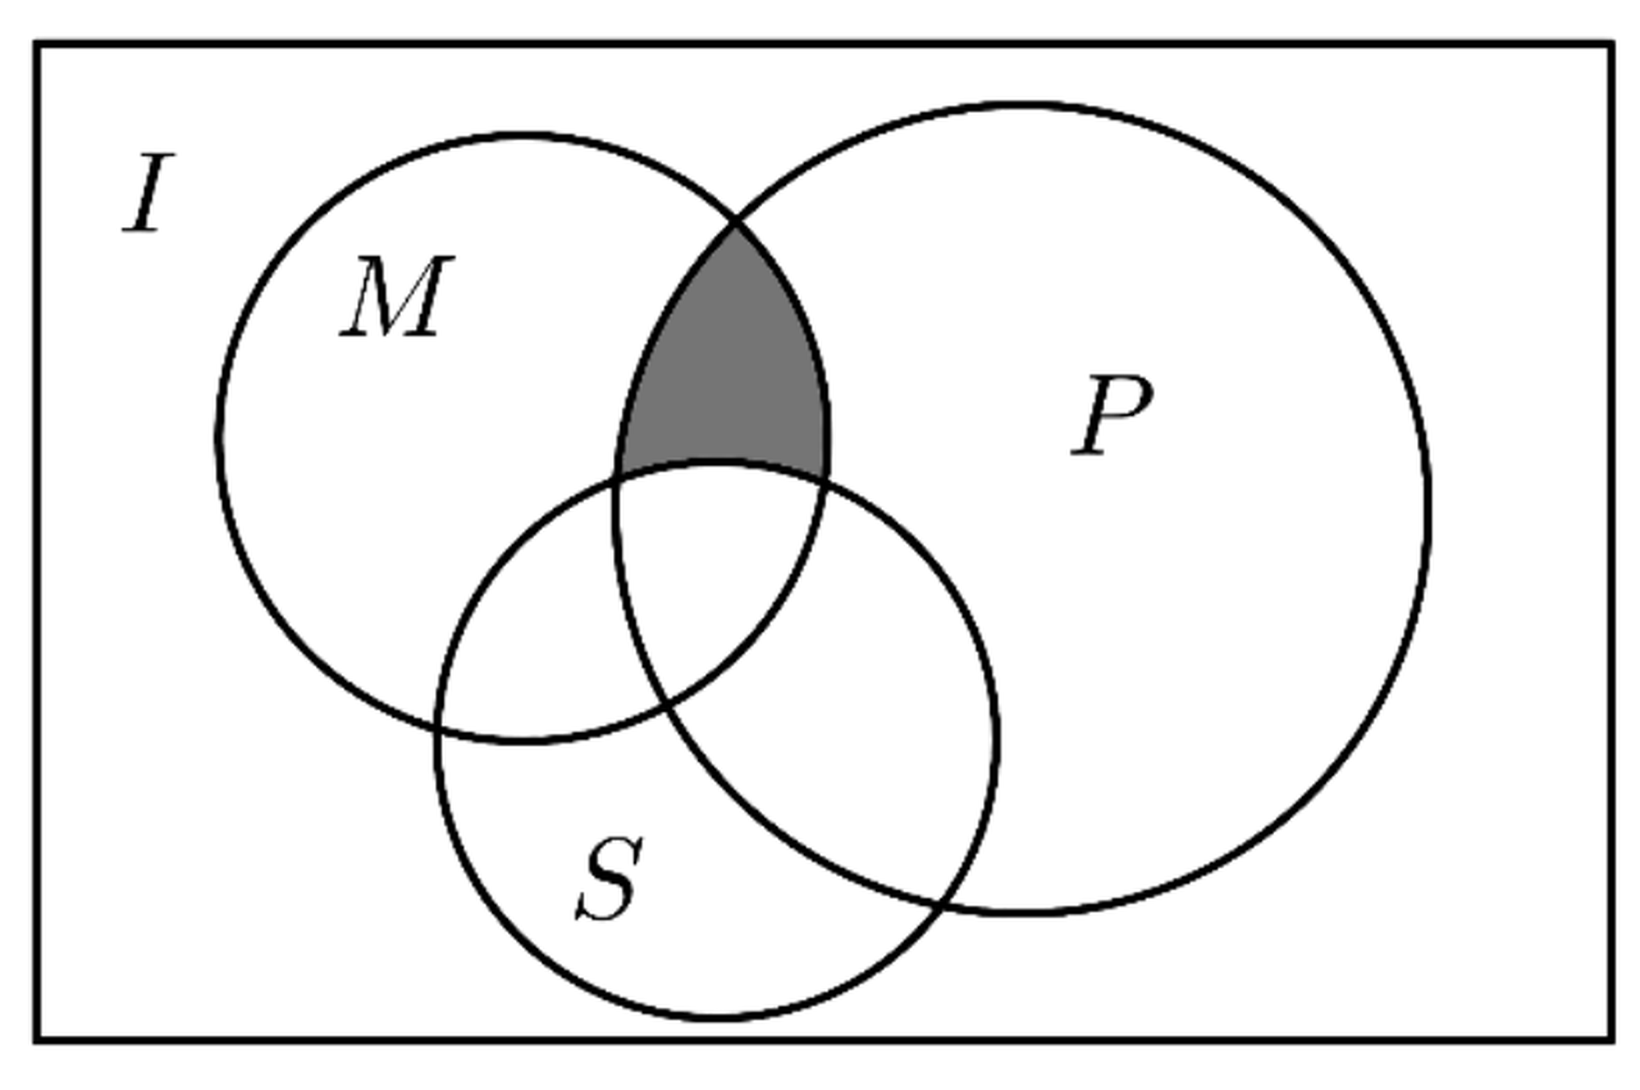
\includegraphics[width=0.42\textwidth]{figures/gao120_q15.png}
\end{center}

\keepwithprev
A. $(M\cap P)\cap S$\qquad\quad B. $(M\cap P)\cap\complement_{I}S$\qquad\quad C. $(M\cup P)\cap S$\qquad\quad D. $\complement_{I}(M\cap P)\cap S$

\ifanswer
\solbegin
\step{由已知中的 $Venn$ 图得阴影部分的元素属于 $M$，属于 $P$，但不属于 $S$，}
\step{所以阴影部分表示的集合为 $(M\cap P)\cap\complement_{I}S$，故选 $B$.}
\solend
\fi

\item 设集合 $P_1=\{x\mid x^2+ax+1>0\}$，$P_2=\{x\mid x^2+ax+2>0\}$，$Q_1=\{x\mid x^2+x+b>0\}$，$Q_2=\{x\mid x^2+2x+b>0\}$，其中 $a$、$b\in\R$，对于下列两个命题：①存在 $a$，$P_1$ 不是 $P_2$ 的子集；②存在 $b$ 使得 $Q_1$ 是 $Q_2$ 的子集. 下列说法正确的是\mbox{（\quad）}

\keepwithprev
A. ①是真命题，②是假命题\qquad\qquad B. ①是假命题，②是真命题

C. ①②都是真命题\qquad\qquad\qquad D. ①②都是假命题

\ifanswer
\solbegin
\step{对于集合 $P_1=\{x\mid x^2+ax+1>0\}$，$P_2=\{x\mid x^2+ax+2>0\}$，}
\step{得当 $m\in P_1$ 时，即 $m^2+am+1>0$，得 $m^2+am+2>0$，}
\step{即有 $m\in P_2$，得对任意 $a$，$P_1$ 是 $P_2$ 的子集，故①错误；}
\step{对于集合 $Q_1=\{x\mid x^2+x+b>0\}$，$Q_2=\{x\mid x^2+2x+b>0\}$，}
\step{当 $b=6$ 时，$Q_1=\{x\mid x^2+x+6>0\}=\R$，$Q_2=\{x\mid x^2+2x+6>0\}=\R$，}
\step{得 $Q_1$ 是 $Q_2$ 的子集，所以存在 $b$，使得 $Q_1$ 是 $Q_2$ 的子集，故②正确；}
\step{故选 $B$.}
\solend
\fi

\end{enumerate}

\bigsec{三、解答题}

\begin{enumerate}
\setcounter{enumi}{16}

\item (1) 已知 $x$、$y$ 都是实数，比较 $x^2+y^2$ 与 $4x-2y-5$ 的大小.

(2) 求解不等式组 $\begin{cases}x^2-4x+3\geqslant0\\\dfrac{x+3}{2x-1}\geqslant2\end{cases}$.

\ifanswer
\solbegin
\step{(1) $(x^2+y^2)-(4x-2y-5)=x^2-4x+y^2+2y+5=(x-2)^2+(y+1)^2\geqslant0$，}
\step{当 $x=2$，$y=-1$ 时，$x^2+y^2=4x-2y-5$.}
\step{当 $x\neq2$ 或 $y\neq-1$ 时，$x^2+y^2>4x-2y-5$.}
\step{(2) 由 $x^2-4x+3\geqslant0$ 得 $(x-1)(x-3)\geqslant0$，所以 $x\leqslant1$ 或 $x\geqslant3$；}
\step{由 $\dfrac{x+3}{2x-1}\geqslant2$，得 $\dfrac{x+3}{2x-1}-2=\dfrac{-3x+5}{2x-1}\geqslant0$，即 $\dfrac{3x-5}{2x-1}\leqslant0$，}
\step{所以 $\begin{cases}(3x-5)(2x-1)\leqslant0\\2x-1\neq0\end{cases}$，解得 $\dfrac12<x\leqslant\dfrac53$，}
\step{所以不等式组的解集是 $\left\{x\,\middle\vert\,\dfrac12<x\leqslant1\right\}$.}
\solend
\fi

\item 已知 $x_1$,$x_2$ 是一元二次方程 $4kx^2-4kx+k+1=0$ 的两个实数根.

(1) 是否存在实数 $k$，$(2x_1-x_2)(x_1-2x_2)=-\dfrac32$ 成立？若存在，求出 $k$ 的值；若不存在，请说明理由.

(2) 求使 $\dfrac{x_1}{x_2}+\dfrac{x_2}{x_1}-2$ 的值为整数的实数 $k$ 的整数值.

\ifanswer
\solbegin
\step{(1) 因为 $x_1$,$x_2$ 是一元二次方程 $4kx^2-4kx+k+1=0$ 的两个实数根，}
\step{所以 $\begin{cases}k\neq0\\16k^2-16k(k+1)\geqslant0\end{cases}$，所以 $k<0$，}
\step{由根与系数的关系得 $x_1+x_2=1$，$x_1x_2=\dfrac{k+1}{4k}$，}
\step{所以 $(2x_1-x_2)(x_1-2x_2)=2(x_1+x_2)^2-9x_1x_2=2-9\times\dfrac{k+1}{4k}=-\dfrac32$，}
\step{解得 $k=\dfrac95$，而 $k<0$，故不存在实数 $k$ 使得 $(2x_1-x_2)(x_1-2x_2)=-\dfrac32$ 成立.}
\step{(2) 由根与系数的关系得 $\dfrac{x_1}{x_2}+\dfrac{x_2}{x_1}-2=\dfrac{(x_1+x_2)^2}{x_1x_2}-4=-\dfrac4{k+1}$，}
\step{因为 $-\dfrac4{k+1}$ 的值为整数，而 $k$ 为整数，所以 $k+1$ 只能取 $\pm1$、$\pm2$、$\pm4$，}
\step{又 $k<0$，所以整数 $k$ 的值为 $-2$ 或 $-3$ 或 $-5$.}
\solend
\fi

\item 2026 年，某市低空经济蓬勃发展，一家物流企业开通“无人机即时配送”服务，并设立配送站. 经市场调研，该站每日配送单量 $y$（单位：单）与每单配送费 $x$（单位：元）满足关系式 $y=4800-200x$（其中 $4<x<24$）. 已知配送站每日的固定成本为 $19200$ 元，每完成一单配送，需支付电费、耗材费、设备保养费等可变成本，每单可变成本为 $4$ 元.

(1) 若要保证配送站每日利润 $W$（单位：元）不为负数，求每单配送费 $x$ 的取值范围；（每日利润 $=$ 每日配送总收入 $-$ 每日可变总成本 $-$ 每日固定成本）

(2) 为提升运力，该站购进一批新型无人机，购机费用为 $32$ 万元. 投入使用后，这批无人机使用 $t(t>0)$ 年的累计维保总费用为 $(2t^2+8t)$ 万元. 请问：这批无人机使用多少年后更新，可以使年平均总费用最低？请求出最低年平均总费用.（年平均总费用 $=$（购机费用 $+$ 维保总费用）$\div$ 使用年数）

\ifanswer
\solbegin
\step{(1) $W=xy-4y-19200=x(4800-200x)-4(4800-200x)-19200$}
\step{$=-200x^2+5600x-38400(4<x<24)$，}
\step{令 $W=-200x^2+5600x-38400\geqslant0$，即 $x^2-28x+192\leqslant0$，}
\step{解得 $12\leqslant x\leqslant16$，因此，要保证配送站每日利润 $W$ 不为负数，}
\step{每单配送费 $x$ 的取值范围为 $[12,16]$；}
\step{(2) 由题意，年平均总费用为 $N=\dfrac{2t^2+8t+32}{t}=2t+\dfrac{32}{t}+8$}
\step{$\geqslant2\sqrt{2t\cdot\dfrac{32}{t}}+8=16+8=24$，当且仅当 $2t=\dfrac{32}{t}$，即 $t=4$ 时取等号，}
\step{则这批无人机使用 $4$ 年后更新，可以使年平均总费用最低，}
\step{最低年平均总费用为 $24$ 万元.}
\solend
\fi

\item 已知 $A,B$，定义集合 $M_{(A,B)}=\{x\mid A<B\}$.

(1) 设 $A=\lvert x-4\rvert$,$B=2x$，求 $M_{(A,B)}$；

(2) 设 $A=ax^2+2ax-4$,$B=2x(x+2)$，当 $M_{(A,B)}=\R$ 时，求 $a$ 的取值范围；

(3) 设 $A=\lvert 2x-b\rvert$,$B=\dfrac{x+4b}{x-1}$,$C=2$，若 $M_{(A,C)}\cap M_{(B,C)}\neq\varnothing$，求 $b$ 的取值范围.

\ifanswer
\solbegin
\step{(1) 由定义，$x\in M_{(A,B)}$ 等价于 $\lvert x-4\rvert<2x$，}
\step{原不等式等价于 $-2x<x-4<2x$，即同时满足 $3x>4$ 与 $x>-4$，}
\step{解得 $x>\dfrac43$，所以 $M_{(A,B)}=\left(\dfrac43,+\infty\right)$.}
\step{(2) 由 $M_{(A,B)}=\R$，得 $ax^2+2ax-4<2x(x+2)$ 对任意 $x\in\R$ 恒成立，}
\step{得 $(a-2)(x+1)^2-a-2<0$.}
\step{当 $a>2$ 时，随着 $(x+1)^2$ 增大，左边可取正值，不符合题意；}
\step{当 $a=2$ 时，左边恒等于 $-4$，符合题意；}
\step{当 $a<2$ 时，左边在 $x=-1$ 处取得最大值 $-a-2$，}
\step{故恒成立的充要条件为 $-a-2<0$，即 $a>-2$；}
\step{综上，$a\in(-2,2]$.}
\step{(3) 由 $\lvert 2x-b\rvert<2$，得 $M_{(A,C)}=\left(\dfrac b2-1,\dfrac b2+1\right)$，记为 $I$.}
\step{由 $\dfrac{x+4b}{x-1}<2$，得 $\dfrac{x-(4b+2)}{x-1}>0$，其中 $x\neq1$.}
\step{①当 $b<-\dfrac14$ 时，$4b+2<1$，故 $M_{(B,C)}=(-\infty,4b+2)\cup(1,+\infty)$.}
\step{此时 $\dfrac b2+1<1$，所以 $I$ 与 $(1,+\infty)$ 没有公共元素.}
\step{两集合交集非空等价于 $\dfrac b2-1<4b+2$，解得 $b>-\dfrac67$.}
\step{因而本种情况得到 $-\dfrac67<b<-\dfrac14$.}
\step{②当 $b=-\dfrac14$ 时，$\dfrac{x+4b}{x-1}=1$，其中 $x\neq1$，故 $M_{(B,C)}=\{x\mid x\neq1\}$.}
\step{此时 $I=\left(-\dfrac98,\dfrac78\right)$，两集合交集非空.}
\step{③当 $b>-\dfrac14$ 时，$4b+2>1$，故 $M_{(B,C)}=(-\infty,1)\cup(4b+2,+\infty)$.}
\step{此时 $4b+2-\left(\dfrac b2+1\right)=\dfrac{7b}{2}+1>\dfrac18>0$，}
\step{所以 $I$ 与 $(4b+2,+\infty)$ 没有公共元素.}
\step{两集合交集非空等价于 $\dfrac b2-1<1$，解得 $b<4$.}
\step{因而本种情况得到 $-\dfrac14<b<4$.}
\step{综上，$b\in\left(-\dfrac67,4\right)$.}
\solend
\fi

\item 破晓同学阅读课外书籍时，发现笛卡尔积是代数和图论中一个很重要的课题. 对于非空数集 $A,B$，定义 $A\otimes B=\{(x,y)\mid x\in A$ 且 $y\in B\}$，将 $A\otimes B$ 称为“$A$ 与 $B$ 的笛卡尔积”.

(1) 若 $A=\{-1,0,1\}$,$B=\{-1,1\}$，求 $A\otimes B$ 和 $B\otimes A$；

(2) 试证明：“$A_1\otimes A_2=A_2\otimes A_1$”是“$A_1=A_2$”的充要条件；

(3) 若集合 $H$ 是有限集，将集合 $H$ 的元素个数记为 $\lvert H\rvert$. 已知 $\lvert A_1\otimes A_2\rvert=m^3(m\in\N^*)$，且存在实数 $a$ 满足 $\sqrt{\dfrac{\lvert A_1\otimes A_1\rvert+\lvert A_2\otimes A_2\rvert}{\lvert A_2\otimes A_1\rvert}}\geqslant a$ 对任意 $m\in\N^*$ 恒成立. 求 $a$ 的取值范围，并指明当 $a$ 取到最值时 $\lvert A_1\rvert$ 和 $\lvert A_2\rvert$ 满足的关系式及 $m$ 应满足的条件.

\ifanswer
\solbegin
\step{(1) 由题意得 $A\otimes B=\{(-1,-1),(-1,1),(0,-1),(0,1),(1,-1),(1,1)\}$，}
\step{$B\otimes A=\{(-1,-1),(-1,0),(-1,1),(1,-1),(1,0),(1,1)\}$；}
\step{(2) 若 $A_1=A_2$，设 $A_1=A_2=A$，}
\step{由定义得 $A_1\otimes A_2=\{(a,b)\mid a\in A$ 且 $b\in A\}=A_2\otimes A_1$，}
\step{所以“$A_1\otimes A_2=A_2\otimes A_1$”是“$A_1=A_2$”的必要条件；}
\step{若 $A_1\otimes A_2=A_2\otimes A_1$，对任意 $(a,b)\in A_1\otimes A_2$，均有 $(a,b)\in A_2\otimes A_1$，}
\step{即对任意 $a\in A_1,b\in A_2$，均有 $a\in A_2,b\in A_1$，}
\step{由任意性得 $A_1\subseteq A_2,A_2\subseteq A_1$，则 $A_1=A_2$，}
\step{所以“$A_1\otimes A_2=A_2\otimes A_1$”是“$A_1=A_2$”的充分条件；}
\step{综上所述，“$A_1\otimes A_2=A_2\otimes A_1$”是“$A_1=A_2$”的充要条件.}
\step{(3) 设 $\lvert A_1\rvert=c$,$\lvert A_2\rvert=d$,$c,d\in\N^*$，}
\step{则 $\lvert A_1\otimes A_2\rvert=\lvert A_2\otimes A_1\rvert=cd=m^3$,$\lvert A_1\otimes A_1\rvert=c^2$,$\lvert A_2\otimes A_2\rvert=d^2$，}
\step{得 $\sqrt{\dfrac{\lvert A_1\otimes A_1\rvert+\lvert A_2\otimes A_2\rvert}{\lvert A_2\otimes A_1\rvert}}=\sqrt{\dfrac{c^2+d^2}{cd}}=\sqrt{\dfrac cd+\dfrac dc}\geqslant\sqrt{2\sqrt{\dfrac cd\cdot\dfrac dc}}=\sqrt2$，}
\step{当且仅当 $\dfrac cd=\dfrac dc$，即 $c=d$ 时取等号，所以实数 $a$ 的取值范围是 $(-\infty,\sqrt2]$.}
\step{若 $a$ 取到最大值，则 $c=d$，即 $\lvert A_1\rvert=\lvert A_2\rvert$，得 $c^2=m^3$，}
\step{即 $c=\sqrt{m^3}=(\sqrt m)^3\in\N^*$，所以 $m=k^2,k\in\N^*$.}
\solend
\fi

\end{enumerate}

\end{document}
"
% 紧凑版：xelatex "\def\iscompact{1}% 高一120_松江二中_10月月考.tex
%   —— 高一上数学“2026-2027 年松江二中高一上 10 月月考”（试卷版/答案版）
% 试卷版：xelatex 高一120_松江二中_10月月考.tex
% 答案版：xelatex "\def\isanswer{1}\input{高一120_松江二中_10月月考.tex}"
% 紧凑版：xelatex "\def\iscompact{1}\input{高一120_松江二中_10月月考.tex}"
%
% 原始材料：微信公众号“魔都数学加油站”文章，作者破晓，2026-11-08 21:35 发布；
% 连载“27学年高一120”，原文标题“27学年高一120——2026-2027年上海市松江二中高一上10月月考”；
% 原文链接：https://mp.weixin.qq.com/s/hgDkaZX9M_IKhmr7CjQc1A。
% 正文为 10 张 PNG 页（第 8、10 页 2560×3620，其余 4762×6735），
% 题目下印有【解析】或【答案】，为讲评版。
% 题目、解析均据原图转录；卷面红色水印及公众号页脚未录入。
% 全卷 1 张插图：第 15 题的三集合 Venn 图（原卷印在题干右侧，本稿移至题干之后，
% 取原卷截图 2× LANCZOS 放大，见 figures/gao120_q15.png）。
%
% 卷首标题：原卷印作“2026-2027 年松江二中高一上 10 月月考”（公众号标题中的“上海市”
% 卷面标题行没有，本稿照卷面），年份区间按全稿惯例排 en dash；原卷未印副标题，本稿按题目内容
% 标为“集合与常用逻辑用语、不等式”（与 110／111／113／116／118 同）。
%
% 与原卷的排版差异：
%   ① 原文从第 3 题起，填空题编号为 3—12、选择题为 13—16、解答题为 17—21，本稿保留原题号；
%   ② 原卷每题下直接印【解析】／【答案】，本稿按全稿惯例置于答案版；第 3 题只印【答案】、
%      第 13、14 题把答案印在题干括号内且无【解析】，均另提 \ans{}；其余选择题答案在
%      解析末句“故选 …”，括号内留空；
%   ③ 原卷未印副标题，本稿按“知识模块”口径补出；
%   ④ 原卷填空横线按全稿惯例排为 \blankline[4.4em]；选择题括号排 \mbox{（\quad）}、
%      选项段前按惯例加 \keepwithprev；解答题不留作答区（原卷为讲评版，与 109—119 同）；
%   ⑤ 原卷数集排斜体 $R$、$N^*$，按全稿惯例改 \R、\N^*；绝对值排 \lvert…\rvert，
%      集合描述竖线排 \mid；补集记号照原卷排 \complement_I。
%
% 判别式字形：第 9 题解析作 $\triangle$（等边、扁），照录 \triangle。
%
% 子集符号：第 4 题题干与解析的 $A\subseteq B$、第 21 题 (2) 的 $A_1\subseteq A_2$ 印有下划线，
%   照录 \subseteq。
%
% 原卷存疑照录：第 12 题题干 $S=\{82,83,84,85,86,87,89\}$ 跳过 $88$ 只列 7 个数，
%   与其“8 种不同的值”自洽（不含 $88$），照录；第 19 题 (1) 的 $W$ 表达式
%   $x(4800-200x)-4(4800-200x)-19200$ 与最后结果 $[12,16]$ 一致。
%
% 行数核对：逐题数 \step 条数，合计 115 条（Q3：0；Q4：4；Q5：2；Q6：5；Q7：4；
% Q8：2；Q9：5；Q10：3；Q11：6；Q12：11；Q13：0；Q14：0；Q15：2；Q16：7；
% Q17：7；Q18：8；Q19：9；Q20：24；Q21：16），与原卷印刷行逐题相等
% （cases 块作一个印刷行计）。第 3 题只印【答案】、第 13、14 题括号内印答案且无解析，
% 均提 \ans{}，不计入 \step 账。
%
\documentclass[a4paper,11pt]{article}
\usepackage{common}

\begin{document}

\examtitlest[3]{2026--2027 年松江二中高一上 10 月月考}{集合与常用逻辑用语、不等式}

\bigsec{一、填空题}

\begin{enumerate}
\setcounter{enumi}{2}

\item 集合 $A=\{(x,y)\mid x+y=8\}$,$B=\{(x,y)\mid xy=12\}$，求 $A\cap B=$\blankline[4.4em].

\ifanswer
\ans{$\{(2,6),(6,2)\}$}
\fi

\item 设集合 $A=\{0,-a\}$,$B=\{1,a-2,2a-2\}$，若 $A\subseteq B$，则 $a=$\blankline[4.4em].

\ifanswer
\solbegin
\step{因为 $A\subseteq B$，}
\step{若 $a-2=0$，解得 $a=2$，此时 $A=\{0,-2\}$,$B=\{1,0,2\}$，不符合题意；}
\step{若 $2a-2=0$，解得 $a=1$，此时 $A=\{0,-1\}$,$B=\{1,-1,0\}$，符合题意；}
\step{综上所述，$a=1$.}
\solend
\fi

\item 设 $\alpha:0<x<a(a>0)$,$\beta:x<8-3a$，若 $\alpha$ 是 $\beta$ 的充分条件，则实数 $a$ 的取值范围是\blankline[4.4em].

\ifanswer
\solbegin
\step{由 $\alpha$ 是 $\beta$ 的充分条件得，$x\in(0,a)\Rightarrow x\in(-\infty,8-3a)$，}
\step{所以 $0<a\leqslant8-3a$，解得 $0<a\leqslant2$.}
\solend
\fi

\item 关于 $x$ 的不等式 $ax-b>0$ 的解集为 $(-\infty,1)$，则不等式 $\dfrac{x-2}{ax+b}<0$ 的解集为\blankline[4.4em].

\ifanswer
\solbegin
\step{因为关于 $x$ 的不等式 $ax-b>0$ 的解集为 $(-\infty,1)$，}
\step{所以 $a<0$ 且 $\dfrac ba=1$，则 $b=a$，}
\step{所以不等式 $\dfrac{x-2}{ax+b}<0$，即 $\dfrac{x-2}{ax+a}<0$，即 $\dfrac{x-2}{x+1}>0$，}
\step{等价于 $(x+1)(x-2)>0$，解得 $x>2$ 或 $x<-1$，}
\step{即解集为 $(-\infty,-1)\cup(2,+\infty)$.}
\solend
\fi

\item 若正实数 $x$、$y$ 满足 $2x+y+8xy=2$，则 $xy$ 的最大值为\blankline[4.4em].

\ifanswer
\solbegin
\step{因为正实数 $x$、$y$ 满足 $2x+y+8xy=2$，}
\step{所以 $2-8xy=2x+y\geqslant2\sqrt{2xy}$，}
\step{当且仅当 $y=2x$，即 $x=\dfrac14$，$y=\dfrac12$ 时取等号，解得 $0<xy\leqslant\dfrac18$，}
\step{故 $xy$ 的最大值为 $\dfrac18$.}
\solend
\fi

\item 已知 $1<a<3$，$-5<b<-2$，则 $\dfrac ab$ 的取值范围是\blankline[4.4em].

\ifanswer
\solbegin
\step{因为 $-5<b<-2$，所以 $2<-b<5$，$\dfrac15<-\dfrac1b<\dfrac12$，又 $1<a<3$，}
\step{得 $\dfrac15<-\dfrac ab<\dfrac32$，则 $-\dfrac32<\dfrac ab<-\dfrac15$，故 $\dfrac ab$ 的取值范围是 $\left(-\dfrac32,-\dfrac15\right)$.}
\solend
\fi

\item 若关于 $x$、$y$ 的方程组 $\begin{cases}y-kx-2=0\\y^2-4x-2y+1=0\end{cases}$ 的解集中只有一个元素，则实数 $k$ 的值为\blankline[4.4em].

\ifanswer
\solbegin
\step{由 $\begin{cases}y-kx-2=0\\y^2-4x-2y+1=0\end{cases}$ 消去 $y$ 整理得 $k^2x^2+(2k-4)x+1=0$.}
\step{当 $k\neq0$ 时，则 $\triangle=(2k-4)^2-4k^2=0$，解得 $k=1$，}
\step{此时方程组的解为 $\begin{cases}x=1\\y=3\end{cases}$，符合题意；}
\step{当 $k=0$ 时，解得 $x=\dfrac14$，此时方程组的解为 $\begin{cases}x=\dfrac14\\y=2\end{cases}$，符合题意；}
\step{综上，$k=0$ 或 $k=1$.}
\solend
\fi

\item 若集合 $A=\{0,1\}$，$B=\{x\mid x^2-mx-m>0,x\in\R\}$，且 $A\cap B=\{1\}$，则实数 $m$ 的取值范围为\blankline[4.4em].

\ifanswer
\solbegin
\step{因为集合 $A=\{0,1\}$，$B=\{x\mid x^2-mx-m>0,x\in\R\}$，且 $A\cap B=\{1\}$，}
\step{则 $1\in B$ 且 $0\notin B$，所以 $\begin{cases}1-m-m>0\\-m\leqslant0\end{cases}$，解得 $0\leqslant m<\dfrac12$，}
\step{所以实数 $m$ 的取值范围是 $\left[0,\dfrac12\right)$.}
\solend
\fi

\item 从集合 $U=\{a,b,c,d\}$ 的子集中选出两个不同的子集，需同时满足以下两个条件：(1) $a$、$b$ 都至少属于其中一个集合；(2) 对选出的两个子集，其中一个集合为另一个的子集，那么共有\blankline[4.4em]种不同的选法.

\ifanswer
\solbegin
\step{不妨设元素少的为 $A$，元素多的为 $B$，则 $B$ 必包含有 $a$、$b$；$A$ 为 $B$ 的真子集，}
\step{若 $B=\{a,b\}$，$A$ 为 $B$ 的真子集，共 $2^2-1=3$ 种，}
\step{若 $B=\{a,b,c\}$，$A$ 为 $B$ 的真子集，共 $2^3-1=7$ 种，}
\step{若 $B=\{a,b,d\}$，$A$ 为 $B$ 的真子集，共 $2^3-1=7$ 种，}
\step{若 $B=\{a,b,c,d\}$，$A$ 为 $B$ 的真子集，共 $2^4-1=15$ 种，}
\step{共有 $3+7+7+15=32$ 种.}
\solend
\fi

\item 已知 $a_1$、$a_2$、$\cdots$、$a_8$ 是 $8$ 个正整数，记 $S=\{a_{i_1}+a_{i_2}+\cdots+a_{i_7}\mid 1\leqslant i_1<i_2<\cdots<i_7\leqslant8\}$，其中 $i_1$、$i_2$、$\cdots$、$i_7\in\N^*$，若 $S=\{82,83,84,85,86,87,89\}$，则这 $8$ 个正整数中的最大数与最小数的积为\blankline[4.4em].

\ifanswer
\solbegin
\step{由题意得从 $8$ 个数中任取 $7$ 个数的和共有 $C_8^7=8$ 种不同的值，}
\step{但是 $82$，$83$，$84$，$85$，$86$，$87$，$89$ 只有 $7$ 个数，}
\step{得必有两种 $7$ 个数的和相等，设这个和为 $t(82\leqslant t\leqslant89)$，}
\step{令 $T=\sum\limits_{i=1}^{8}a_i$，那么，任取 $7$ 个数的和就等于 $T-a_i$，$i=1,2,\cdots,8$，}
\step{这 $8$ 个取值和的集合为 $S$，$S=\{T-a_1,T-a_2,\cdots,T-a_8\}$，}
\step{则 $\sum\limits_{i=1}^{8}(T-a_i)=8T-T=7T=82+83+84+85+86+87+89+t=596+t$.}
\step{因为 $T$ 为整数，所以 $596+t$ 是 $7$ 的倍数，}
\step{由 $596=7\times85+1$ 得 $1+t$ 是 $7$ 的倍数，}
\step{再因为 $82\leqslant t\leqslant89$，所以 $t=83$，得 $T=97$.}
\step{因此 $a_1$、$a_2$、$\cdots$、$a_8$ 中最大数为 $97-82=15$，最小数为 $97-89=8$，}
\step{因此，它们的积为 $120$.}
\solend
\fi

\end{enumerate}

\bigsec{二、选择题}

\begin{enumerate}
\setcounter{enumi}{12}

\item 已知 $a>b>0$，$c\in\R$，则下列不等式不一定成立的是\mbox{（\quad）}% 原卷把答案“$B$”印在题干括号内、无【解析】

\keepwithprev
A. $a-c>b-c$\qquad\quad B. $ac>bc$\qquad\quad C. $\dfrac1a<\dfrac1b$\qquad\quad D. $\dfrac{a+b}{2}>\sqrt{ab}$

\ifanswer
\ans{$B$}
\fi

\item 命题“对任意的 $x\in\R,x^3-x^2+1\leqslant0$”的否定是\mbox{（\quad）}% 原卷把答案“$C$”印在题干括号内、无【解析】

\keepwithprev
A. 不存在 $x\in\R,x^3-x^2+1\leqslant0$\qquad B. 存在 $x\in\R,x^3-x^2+1\leqslant0$

C. 存在 $x\in\R,x^3-x^2+1>0$\qquad\quad D. 对任意的 $x\in\R,x^3-x^2+1>0$

\ifanswer
\ans{$C$}
\fi

% 第 15 题是“题干 + 图 + 选项”约 6.5cm 的一整块，\keepwithprev 只挡得住“图—选项”，
% 挡不住夹在中间的图——实测断点落在题干之后（切页审计 A 类）。故照 高一30／高一26 成例
% 在题前先量一次页高，不够就把整块一起挪到次页。
\needvspace{7cm}
\item 如图，$I$ 是全集，$M$、$P$、$S$ 是 $I$ 的三个子集，则阴影部分所表示的集合是\mbox{（\quad）}

\begin{center}
% 图取原卷截图（第 4 页题干右侧）、2× LANCZOS 放大，本稿移至题干之后
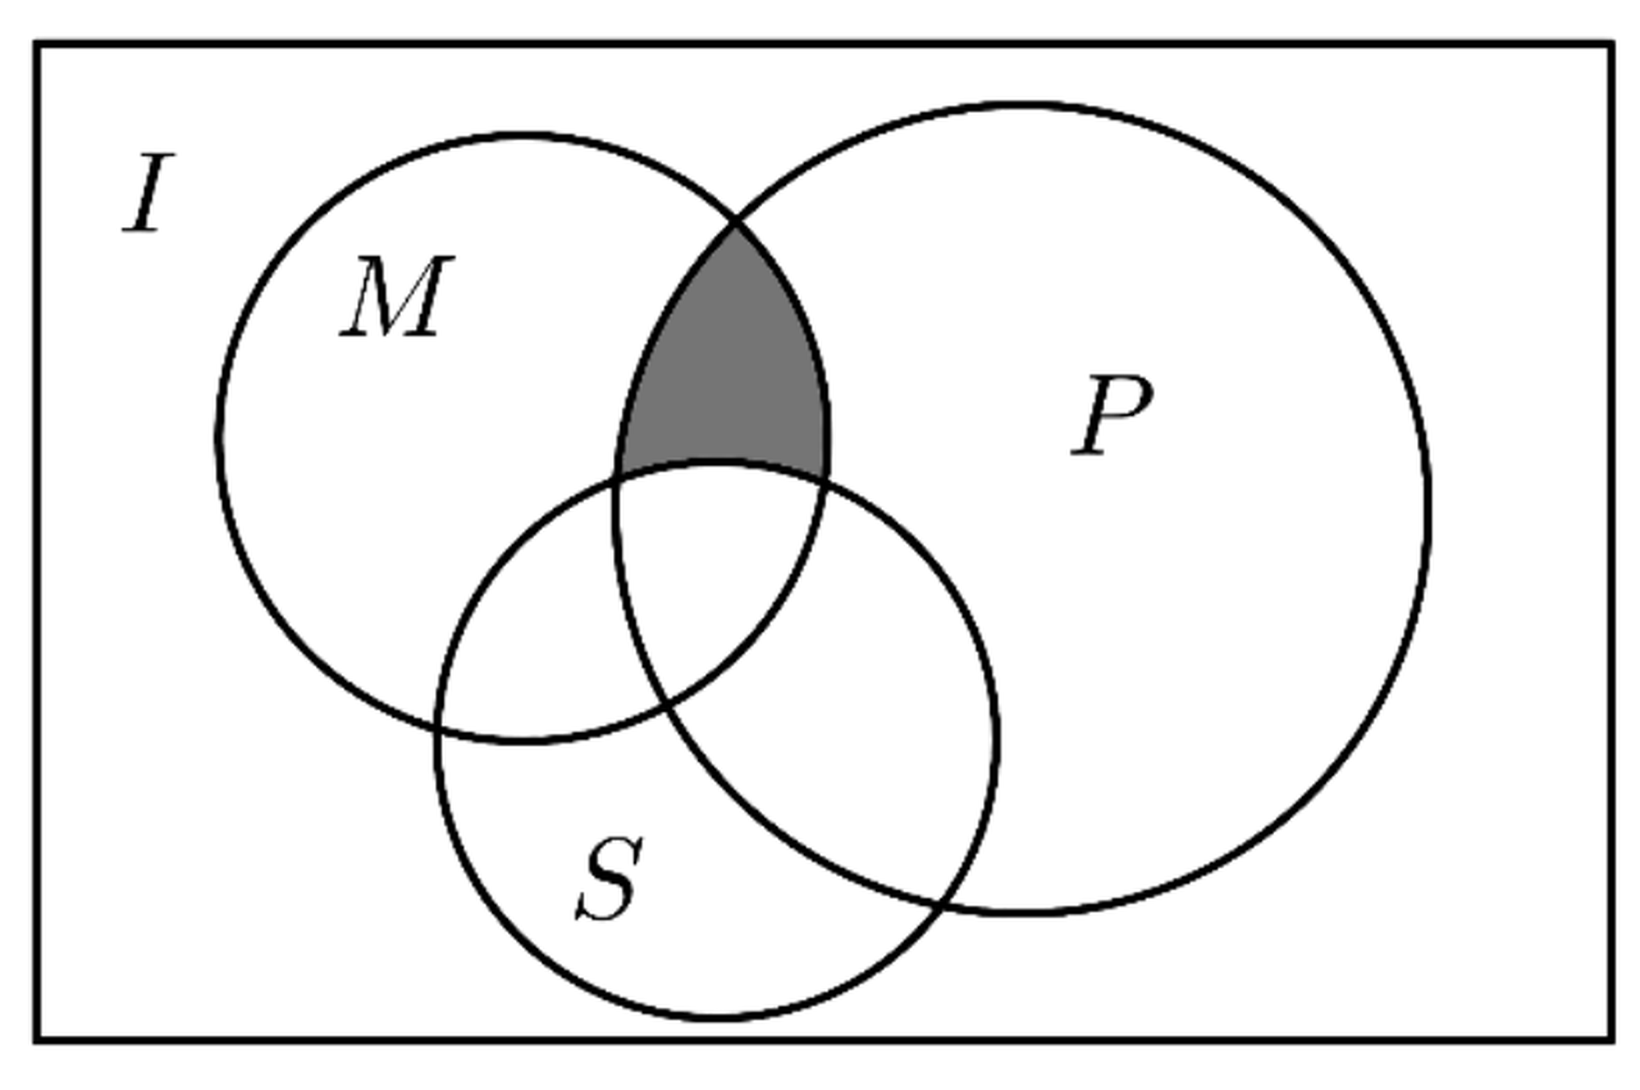
\includegraphics[width=0.42\textwidth]{figures/gao120_q15.png}
\end{center}

\keepwithprev
A. $(M\cap P)\cap S$\qquad\quad B. $(M\cap P)\cap\complement_{I}S$\qquad\quad C. $(M\cup P)\cap S$\qquad\quad D. $\complement_{I}(M\cap P)\cap S$

\ifanswer
\solbegin
\step{由已知中的 $Venn$ 图得阴影部分的元素属于 $M$，属于 $P$，但不属于 $S$，}
\step{所以阴影部分表示的集合为 $(M\cap P)\cap\complement_{I}S$，故选 $B$.}
\solend
\fi

\item 设集合 $P_1=\{x\mid x^2+ax+1>0\}$，$P_2=\{x\mid x^2+ax+2>0\}$，$Q_1=\{x\mid x^2+x+b>0\}$，$Q_2=\{x\mid x^2+2x+b>0\}$，其中 $a$、$b\in\R$，对于下列两个命题：①存在 $a$，$P_1$ 不是 $P_2$ 的子集；②存在 $b$ 使得 $Q_1$ 是 $Q_2$ 的子集. 下列说法正确的是\mbox{（\quad）}

\keepwithprev
A. ①是真命题，②是假命题\qquad\qquad B. ①是假命题，②是真命题

C. ①②都是真命题\qquad\qquad\qquad D. ①②都是假命题

\ifanswer
\solbegin
\step{对于集合 $P_1=\{x\mid x^2+ax+1>0\}$，$P_2=\{x\mid x^2+ax+2>0\}$，}
\step{得当 $m\in P_1$ 时，即 $m^2+am+1>0$，得 $m^2+am+2>0$，}
\step{即有 $m\in P_2$，得对任意 $a$，$P_1$ 是 $P_2$ 的子集，故①错误；}
\step{对于集合 $Q_1=\{x\mid x^2+x+b>0\}$，$Q_2=\{x\mid x^2+2x+b>0\}$，}
\step{当 $b=6$ 时，$Q_1=\{x\mid x^2+x+6>0\}=\R$，$Q_2=\{x\mid x^2+2x+6>0\}=\R$，}
\step{得 $Q_1$ 是 $Q_2$ 的子集，所以存在 $b$，使得 $Q_1$ 是 $Q_2$ 的子集，故②正确；}
\step{故选 $B$.}
\solend
\fi

\end{enumerate}

\bigsec{三、解答题}

\begin{enumerate}
\setcounter{enumi}{16}

\item (1) 已知 $x$、$y$ 都是实数，比较 $x^2+y^2$ 与 $4x-2y-5$ 的大小.

(2) 求解不等式组 $\begin{cases}x^2-4x+3\geqslant0\\\dfrac{x+3}{2x-1}\geqslant2\end{cases}$.

\ifanswer
\solbegin
\step{(1) $(x^2+y^2)-(4x-2y-5)=x^2-4x+y^2+2y+5=(x-2)^2+(y+1)^2\geqslant0$，}
\step{当 $x=2$，$y=-1$ 时，$x^2+y^2=4x-2y-5$.}
\step{当 $x\neq2$ 或 $y\neq-1$ 时，$x^2+y^2>4x-2y-5$.}
\step{(2) 由 $x^2-4x+3\geqslant0$ 得 $(x-1)(x-3)\geqslant0$，所以 $x\leqslant1$ 或 $x\geqslant3$；}
\step{由 $\dfrac{x+3}{2x-1}\geqslant2$，得 $\dfrac{x+3}{2x-1}-2=\dfrac{-3x+5}{2x-1}\geqslant0$，即 $\dfrac{3x-5}{2x-1}\leqslant0$，}
\step{所以 $\begin{cases}(3x-5)(2x-1)\leqslant0\\2x-1\neq0\end{cases}$，解得 $\dfrac12<x\leqslant\dfrac53$，}
\step{所以不等式组的解集是 $\left\{x\,\middle\vert\,\dfrac12<x\leqslant1\right\}$.}
\solend
\fi

\item 已知 $x_1$,$x_2$ 是一元二次方程 $4kx^2-4kx+k+1=0$ 的两个实数根.

(1) 是否存在实数 $k$，$(2x_1-x_2)(x_1-2x_2)=-\dfrac32$ 成立？若存在，求出 $k$ 的值；若不存在，请说明理由.

(2) 求使 $\dfrac{x_1}{x_2}+\dfrac{x_2}{x_1}-2$ 的值为整数的实数 $k$ 的整数值.

\ifanswer
\solbegin
\step{(1) 因为 $x_1$,$x_2$ 是一元二次方程 $4kx^2-4kx+k+1=0$ 的两个实数根，}
\step{所以 $\begin{cases}k\neq0\\16k^2-16k(k+1)\geqslant0\end{cases}$，所以 $k<0$，}
\step{由根与系数的关系得 $x_1+x_2=1$，$x_1x_2=\dfrac{k+1}{4k}$，}
\step{所以 $(2x_1-x_2)(x_1-2x_2)=2(x_1+x_2)^2-9x_1x_2=2-9\times\dfrac{k+1}{4k}=-\dfrac32$，}
\step{解得 $k=\dfrac95$，而 $k<0$，故不存在实数 $k$ 使得 $(2x_1-x_2)(x_1-2x_2)=-\dfrac32$ 成立.}
\step{(2) 由根与系数的关系得 $\dfrac{x_1}{x_2}+\dfrac{x_2}{x_1}-2=\dfrac{(x_1+x_2)^2}{x_1x_2}-4=-\dfrac4{k+1}$，}
\step{因为 $-\dfrac4{k+1}$ 的值为整数，而 $k$ 为整数，所以 $k+1$ 只能取 $\pm1$、$\pm2$、$\pm4$，}
\step{又 $k<0$，所以整数 $k$ 的值为 $-2$ 或 $-3$ 或 $-5$.}
\solend
\fi

\item 2026 年，某市低空经济蓬勃发展，一家物流企业开通“无人机即时配送”服务，并设立配送站. 经市场调研，该站每日配送单量 $y$（单位：单）与每单配送费 $x$（单位：元）满足关系式 $y=4800-200x$（其中 $4<x<24$）. 已知配送站每日的固定成本为 $19200$ 元，每完成一单配送，需支付电费、耗材费、设备保养费等可变成本，每单可变成本为 $4$ 元.

(1) 若要保证配送站每日利润 $W$（单位：元）不为负数，求每单配送费 $x$ 的取值范围；（每日利润 $=$ 每日配送总收入 $-$ 每日可变总成本 $-$ 每日固定成本）

(2) 为提升运力，该站购进一批新型无人机，购机费用为 $32$ 万元. 投入使用后，这批无人机使用 $t(t>0)$ 年的累计维保总费用为 $(2t^2+8t)$ 万元. 请问：这批无人机使用多少年后更新，可以使年平均总费用最低？请求出最低年平均总费用.（年平均总费用 $=$（购机费用 $+$ 维保总费用）$\div$ 使用年数）

\ifanswer
\solbegin
\step{(1) $W=xy-4y-19200=x(4800-200x)-4(4800-200x)-19200$}
\step{$=-200x^2+5600x-38400(4<x<24)$，}
\step{令 $W=-200x^2+5600x-38400\geqslant0$，即 $x^2-28x+192\leqslant0$，}
\step{解得 $12\leqslant x\leqslant16$，因此，要保证配送站每日利润 $W$ 不为负数，}
\step{每单配送费 $x$ 的取值范围为 $[12,16]$；}
\step{(2) 由题意，年平均总费用为 $N=\dfrac{2t^2+8t+32}{t}=2t+\dfrac{32}{t}+8$}
\step{$\geqslant2\sqrt{2t\cdot\dfrac{32}{t}}+8=16+8=24$，当且仅当 $2t=\dfrac{32}{t}$，即 $t=4$ 时取等号，}
\step{则这批无人机使用 $4$ 年后更新，可以使年平均总费用最低，}
\step{最低年平均总费用为 $24$ 万元.}
\solend
\fi

\item 已知 $A,B$，定义集合 $M_{(A,B)}=\{x\mid A<B\}$.

(1) 设 $A=\lvert x-4\rvert$,$B=2x$，求 $M_{(A,B)}$；

(2) 设 $A=ax^2+2ax-4$,$B=2x(x+2)$，当 $M_{(A,B)}=\R$ 时，求 $a$ 的取值范围；

(3) 设 $A=\lvert 2x-b\rvert$,$B=\dfrac{x+4b}{x-1}$,$C=2$，若 $M_{(A,C)}\cap M_{(B,C)}\neq\varnothing$，求 $b$ 的取值范围.

\ifanswer
\solbegin
\step{(1) 由定义，$x\in M_{(A,B)}$ 等价于 $\lvert x-4\rvert<2x$，}
\step{原不等式等价于 $-2x<x-4<2x$，即同时满足 $3x>4$ 与 $x>-4$，}
\step{解得 $x>\dfrac43$，所以 $M_{(A,B)}=\left(\dfrac43,+\infty\right)$.}
\step{(2) 由 $M_{(A,B)}=\R$，得 $ax^2+2ax-4<2x(x+2)$ 对任意 $x\in\R$ 恒成立，}
\step{得 $(a-2)(x+1)^2-a-2<0$.}
\step{当 $a>2$ 时，随着 $(x+1)^2$ 增大，左边可取正值，不符合题意；}
\step{当 $a=2$ 时，左边恒等于 $-4$，符合题意；}
\step{当 $a<2$ 时，左边在 $x=-1$ 处取得最大值 $-a-2$，}
\step{故恒成立的充要条件为 $-a-2<0$，即 $a>-2$；}
\step{综上，$a\in(-2,2]$.}
\step{(3) 由 $\lvert 2x-b\rvert<2$，得 $M_{(A,C)}=\left(\dfrac b2-1,\dfrac b2+1\right)$，记为 $I$.}
\step{由 $\dfrac{x+4b}{x-1}<2$，得 $\dfrac{x-(4b+2)}{x-1}>0$，其中 $x\neq1$.}
\step{①当 $b<-\dfrac14$ 时，$4b+2<1$，故 $M_{(B,C)}=(-\infty,4b+2)\cup(1,+\infty)$.}
\step{此时 $\dfrac b2+1<1$，所以 $I$ 与 $(1,+\infty)$ 没有公共元素.}
\step{两集合交集非空等价于 $\dfrac b2-1<4b+2$，解得 $b>-\dfrac67$.}
\step{因而本种情况得到 $-\dfrac67<b<-\dfrac14$.}
\step{②当 $b=-\dfrac14$ 时，$\dfrac{x+4b}{x-1}=1$，其中 $x\neq1$，故 $M_{(B,C)}=\{x\mid x\neq1\}$.}
\step{此时 $I=\left(-\dfrac98,\dfrac78\right)$，两集合交集非空.}
\step{③当 $b>-\dfrac14$ 时，$4b+2>1$，故 $M_{(B,C)}=(-\infty,1)\cup(4b+2,+\infty)$.}
\step{此时 $4b+2-\left(\dfrac b2+1\right)=\dfrac{7b}{2}+1>\dfrac18>0$，}
\step{所以 $I$ 与 $(4b+2,+\infty)$ 没有公共元素.}
\step{两集合交集非空等价于 $\dfrac b2-1<1$，解得 $b<4$.}
\step{因而本种情况得到 $-\dfrac14<b<4$.}
\step{综上，$b\in\left(-\dfrac67,4\right)$.}
\solend
\fi

\item 破晓同学阅读课外书籍时，发现笛卡尔积是代数和图论中一个很重要的课题. 对于非空数集 $A,B$，定义 $A\otimes B=\{(x,y)\mid x\in A$ 且 $y\in B\}$，将 $A\otimes B$ 称为“$A$ 与 $B$ 的笛卡尔积”.

(1) 若 $A=\{-1,0,1\}$,$B=\{-1,1\}$，求 $A\otimes B$ 和 $B\otimes A$；

(2) 试证明：“$A_1\otimes A_2=A_2\otimes A_1$”是“$A_1=A_2$”的充要条件；

(3) 若集合 $H$ 是有限集，将集合 $H$ 的元素个数记为 $\lvert H\rvert$. 已知 $\lvert A_1\otimes A_2\rvert=m^3(m\in\N^*)$，且存在实数 $a$ 满足 $\sqrt{\dfrac{\lvert A_1\otimes A_1\rvert+\lvert A_2\otimes A_2\rvert}{\lvert A_2\otimes A_1\rvert}}\geqslant a$ 对任意 $m\in\N^*$ 恒成立. 求 $a$ 的取值范围，并指明当 $a$ 取到最值时 $\lvert A_1\rvert$ 和 $\lvert A_2\rvert$ 满足的关系式及 $m$ 应满足的条件.

\ifanswer
\solbegin
\step{(1) 由题意得 $A\otimes B=\{(-1,-1),(-1,1),(0,-1),(0,1),(1,-1),(1,1)\}$，}
\step{$B\otimes A=\{(-1,-1),(-1,0),(-1,1),(1,-1),(1,0),(1,1)\}$；}
\step{(2) 若 $A_1=A_2$，设 $A_1=A_2=A$，}
\step{由定义得 $A_1\otimes A_2=\{(a,b)\mid a\in A$ 且 $b\in A\}=A_2\otimes A_1$，}
\step{所以“$A_1\otimes A_2=A_2\otimes A_1$”是“$A_1=A_2$”的必要条件；}
\step{若 $A_1\otimes A_2=A_2\otimes A_1$，对任意 $(a,b)\in A_1\otimes A_2$，均有 $(a,b)\in A_2\otimes A_1$，}
\step{即对任意 $a\in A_1,b\in A_2$，均有 $a\in A_2,b\in A_1$，}
\step{由任意性得 $A_1\subseteq A_2,A_2\subseteq A_1$，则 $A_1=A_2$，}
\step{所以“$A_1\otimes A_2=A_2\otimes A_1$”是“$A_1=A_2$”的充分条件；}
\step{综上所述，“$A_1\otimes A_2=A_2\otimes A_1$”是“$A_1=A_2$”的充要条件.}
\step{(3) 设 $\lvert A_1\rvert=c$,$\lvert A_2\rvert=d$,$c,d\in\N^*$，}
\step{则 $\lvert A_1\otimes A_2\rvert=\lvert A_2\otimes A_1\rvert=cd=m^3$,$\lvert A_1\otimes A_1\rvert=c^2$,$\lvert A_2\otimes A_2\rvert=d^2$，}
\step{得 $\sqrt{\dfrac{\lvert A_1\otimes A_1\rvert+\lvert A_2\otimes A_2\rvert}{\lvert A_2\otimes A_1\rvert}}=\sqrt{\dfrac{c^2+d^2}{cd}}=\sqrt{\dfrac cd+\dfrac dc}\geqslant\sqrt{2\sqrt{\dfrac cd\cdot\dfrac dc}}=\sqrt2$，}
\step{当且仅当 $\dfrac cd=\dfrac dc$，即 $c=d$ 时取等号，所以实数 $a$ 的取值范围是 $(-\infty,\sqrt2]$.}
\step{若 $a$ 取到最大值，则 $c=d$，即 $\lvert A_1\rvert=\lvert A_2\rvert$，得 $c^2=m^3$，}
\step{即 $c=\sqrt{m^3}=(\sqrt m)^3\in\N^*$，所以 $m=k^2,k\in\N^*$.}
\solend
\fi

\end{enumerate}

\end{document}
"
%
% 原始材料：微信公众号“魔都数学加油站”文章，作者破晓，2026-11-08 21:35 发布；
% 连载“27学年高一120”，原文标题“27学年高一120——2026-2027年上海市松江二中高一上10月月考”；
% 原文链接：https://mp.weixin.qq.com/s/hgDkaZX9M_IKhmr7CjQc1A。
% 正文为 10 张 PNG 页（第 8、10 页 2560×3620，其余 4762×6735），
% 题目下印有【解析】或【答案】，为讲评版。
% 题目、解析均据原图转录；卷面红色水印及公众号页脚未录入。
% 全卷 1 张插图：第 15 题的三集合 Venn 图（原卷印在题干右侧，本稿移至题干之后，
% 取原卷截图 2× LANCZOS 放大，见 figures/gao120_q15.png）。
%
% 卷首标题：原卷印作“2026-2027 年松江二中高一上 10 月月考”（公众号标题中的“上海市”
% 卷面标题行没有，本稿照卷面），年份区间按全稿惯例排 en dash；原卷未印副标题，本稿按题目内容
% 标为“集合与常用逻辑用语、不等式”（与 110／111／113／116／118 同）。
%
% 与原卷的排版差异：
%   ① 原文从第 3 题起，填空题编号为 3—12、选择题为 13—16、解答题为 17—21，本稿保留原题号；
%   ② 原卷每题下直接印【解析】／【答案】，本稿按全稿惯例置于答案版；第 3 题只印【答案】、
%      第 13、14 题把答案印在题干括号内且无【解析】，均另提 \ans{}；其余选择题答案在
%      解析末句“故选 …”，括号内留空；
%   ③ 原卷未印副标题，本稿按“知识模块”口径补出；
%   ④ 原卷填空横线按全稿惯例排为 \blankline[4.4em]；选择题括号排 \mbox{（\quad）}、
%      选项段前按惯例加 \keepwithprev；解答题不留作答区（原卷为讲评版，与 109—119 同）；
%   ⑤ 原卷数集排斜体 $R$、$N^*$，按全稿惯例改 \R、\N^*；绝对值排 \lvert…\rvert，
%      集合描述竖线排 \mid；补集记号照原卷排 \complement_I。
%
% 判别式字形：第 9 题解析作 $\triangle$（等边、扁），照录 \triangle。
%
% 子集符号：第 4 题题干与解析的 $A\subseteq B$、第 21 题 (2) 的 $A_1\subseteq A_2$ 印有下划线，
%   照录 \subseteq。
%
% 原卷存疑照录：第 12 题题干 $S=\{82,83,84,85,86,87,89\}$ 跳过 $88$ 只列 7 个数，
%   与其“8 种不同的值”自洽（不含 $88$），照录；第 19 题 (1) 的 $W$ 表达式
%   $x(4800-200x)-4(4800-200x)-19200$ 与最后结果 $[12,16]$ 一致。
%
% 行数核对：逐题数 \step 条数，合计 115 条（Q3：0；Q4：4；Q5：2；Q6：5；Q7：4；
% Q8：2；Q9：5；Q10：3；Q11：6；Q12：11；Q13：0；Q14：0；Q15：2；Q16：7；
% Q17：7；Q18：8；Q19：9；Q20：24；Q21：16），与原卷印刷行逐题相等
% （cases 块作一个印刷行计）。第 3 题只印【答案】、第 13、14 题括号内印答案且无解析，
% 均提 \ans{}，不计入 \step 账。
%
\documentclass[a4paper,11pt]{article}
\usepackage{common}

\begin{document}

\examtitlest[3]{2026--2027 年松江二中高一上 10 月月考}{集合与常用逻辑用语、不等式}

\bigsec{一、填空题}

\begin{enumerate}
\setcounter{enumi}{2}

\item 集合 $A=\{(x,y)\mid x+y=8\}$,$B=\{(x,y)\mid xy=12\}$，求 $A\cap B=$\blankline[4.4em].

\ifanswer
\ans{$\{(2,6),(6,2)\}$}
\fi

\item 设集合 $A=\{0,-a\}$,$B=\{1,a-2,2a-2\}$，若 $A\subseteq B$，则 $a=$\blankline[4.4em].

\ifanswer
\solbegin
\step{因为 $A\subseteq B$，}
\step{若 $a-2=0$，解得 $a=2$，此时 $A=\{0,-2\}$,$B=\{1,0,2\}$，不符合题意；}
\step{若 $2a-2=0$，解得 $a=1$，此时 $A=\{0,-1\}$,$B=\{1,-1,0\}$，符合题意；}
\step{综上所述，$a=1$.}
\solend
\fi

\item 设 $\alpha:0<x<a(a>0)$,$\beta:x<8-3a$，若 $\alpha$ 是 $\beta$ 的充分条件，则实数 $a$ 的取值范围是\blankline[4.4em].

\ifanswer
\solbegin
\step{由 $\alpha$ 是 $\beta$ 的充分条件得，$x\in(0,a)\Rightarrow x\in(-\infty,8-3a)$，}
\step{所以 $0<a\leqslant8-3a$，解得 $0<a\leqslant2$.}
\solend
\fi

\item 关于 $x$ 的不等式 $ax-b>0$ 的解集为 $(-\infty,1)$，则不等式 $\dfrac{x-2}{ax+b}<0$ 的解集为\blankline[4.4em].

\ifanswer
\solbegin
\step{因为关于 $x$ 的不等式 $ax-b>0$ 的解集为 $(-\infty,1)$，}
\step{所以 $a<0$ 且 $\dfrac ba=1$，则 $b=a$，}
\step{所以不等式 $\dfrac{x-2}{ax+b}<0$，即 $\dfrac{x-2}{ax+a}<0$，即 $\dfrac{x-2}{x+1}>0$，}
\step{等价于 $(x+1)(x-2)>0$，解得 $x>2$ 或 $x<-1$，}
\step{即解集为 $(-\infty,-1)\cup(2,+\infty)$.}
\solend
\fi

\item 若正实数 $x$、$y$ 满足 $2x+y+8xy=2$，则 $xy$ 的最大值为\blankline[4.4em].

\ifanswer
\solbegin
\step{因为正实数 $x$、$y$ 满足 $2x+y+8xy=2$，}
\step{所以 $2-8xy=2x+y\geqslant2\sqrt{2xy}$，}
\step{当且仅当 $y=2x$，即 $x=\dfrac14$，$y=\dfrac12$ 时取等号，解得 $0<xy\leqslant\dfrac18$，}
\step{故 $xy$ 的最大值为 $\dfrac18$.}
\solend
\fi

\item 已知 $1<a<3$，$-5<b<-2$，则 $\dfrac ab$ 的取值范围是\blankline[4.4em].

\ifanswer
\solbegin
\step{因为 $-5<b<-2$，所以 $2<-b<5$，$\dfrac15<-\dfrac1b<\dfrac12$，又 $1<a<3$，}
\step{得 $\dfrac15<-\dfrac ab<\dfrac32$，则 $-\dfrac32<\dfrac ab<-\dfrac15$，故 $\dfrac ab$ 的取值范围是 $\left(-\dfrac32,-\dfrac15\right)$.}
\solend
\fi

\item 若关于 $x$、$y$ 的方程组 $\begin{cases}y-kx-2=0\\y^2-4x-2y+1=0\end{cases}$ 的解集中只有一个元素，则实数 $k$ 的值为\blankline[4.4em].

\ifanswer
\solbegin
\step{由 $\begin{cases}y-kx-2=0\\y^2-4x-2y+1=0\end{cases}$ 消去 $y$ 整理得 $k^2x^2+(2k-4)x+1=0$.}
\step{当 $k\neq0$ 时，则 $\triangle=(2k-4)^2-4k^2=0$，解得 $k=1$，}
\step{此时方程组的解为 $\begin{cases}x=1\\y=3\end{cases}$，符合题意；}
\step{当 $k=0$ 时，解得 $x=\dfrac14$，此时方程组的解为 $\begin{cases}x=\dfrac14\\y=2\end{cases}$，符合题意；}
\step{综上，$k=0$ 或 $k=1$.}
\solend
\fi

\item 若集合 $A=\{0,1\}$，$B=\{x\mid x^2-mx-m>0,x\in\R\}$，且 $A\cap B=\{1\}$，则实数 $m$ 的取值范围为\blankline[4.4em].

\ifanswer
\solbegin
\step{因为集合 $A=\{0,1\}$，$B=\{x\mid x^2-mx-m>0,x\in\R\}$，且 $A\cap B=\{1\}$，}
\step{则 $1\in B$ 且 $0\notin B$，所以 $\begin{cases}1-m-m>0\\-m\leqslant0\end{cases}$，解得 $0\leqslant m<\dfrac12$，}
\step{所以实数 $m$ 的取值范围是 $\left[0,\dfrac12\right)$.}
\solend
\fi

\item 从集合 $U=\{a,b,c,d\}$ 的子集中选出两个不同的子集，需同时满足以下两个条件：(1) $a$、$b$ 都至少属于其中一个集合；(2) 对选出的两个子集，其中一个集合为另一个的子集，那么共有\blankline[4.4em]种不同的选法.

\ifanswer
\solbegin
\step{不妨设元素少的为 $A$，元素多的为 $B$，则 $B$ 必包含有 $a$、$b$；$A$ 为 $B$ 的真子集，}
\step{若 $B=\{a,b\}$，$A$ 为 $B$ 的真子集，共 $2^2-1=3$ 种，}
\step{若 $B=\{a,b,c\}$，$A$ 为 $B$ 的真子集，共 $2^3-1=7$ 种，}
\step{若 $B=\{a,b,d\}$，$A$ 为 $B$ 的真子集，共 $2^3-1=7$ 种，}
\step{若 $B=\{a,b,c,d\}$，$A$ 为 $B$ 的真子集，共 $2^4-1=15$ 种，}
\step{共有 $3+7+7+15=32$ 种.}
\solend
\fi

\item 已知 $a_1$、$a_2$、$\cdots$、$a_8$ 是 $8$ 个正整数，记 $S=\{a_{i_1}+a_{i_2}+\cdots+a_{i_7}\mid 1\leqslant i_1<i_2<\cdots<i_7\leqslant8\}$，其中 $i_1$、$i_2$、$\cdots$、$i_7\in\N^*$，若 $S=\{82,83,84,85,86,87,89\}$，则这 $8$ 个正整数中的最大数与最小数的积为\blankline[4.4em].

\ifanswer
\solbegin
\step{由题意得从 $8$ 个数中任取 $7$ 个数的和共有 $C_8^7=8$ 种不同的值，}
\step{但是 $82$，$83$，$84$，$85$，$86$，$87$，$89$ 只有 $7$ 个数，}
\step{得必有两种 $7$ 个数的和相等，设这个和为 $t(82\leqslant t\leqslant89)$，}
\step{令 $T=\sum\limits_{i=1}^{8}a_i$，那么，任取 $7$ 个数的和就等于 $T-a_i$，$i=1,2,\cdots,8$，}
\step{这 $8$ 个取值和的集合为 $S$，$S=\{T-a_1,T-a_2,\cdots,T-a_8\}$，}
\step{则 $\sum\limits_{i=1}^{8}(T-a_i)=8T-T=7T=82+83+84+85+86+87+89+t=596+t$.}
\step{因为 $T$ 为整数，所以 $596+t$ 是 $7$ 的倍数，}
\step{由 $596=7\times85+1$ 得 $1+t$ 是 $7$ 的倍数，}
\step{再因为 $82\leqslant t\leqslant89$，所以 $t=83$，得 $T=97$.}
\step{因此 $a_1$、$a_2$、$\cdots$、$a_8$ 中最大数为 $97-82=15$，最小数为 $97-89=8$，}
\step{因此，它们的积为 $120$.}
\solend
\fi

\end{enumerate}

\bigsec{二、选择题}

\begin{enumerate}
\setcounter{enumi}{12}

\item 已知 $a>b>0$，$c\in\R$，则下列不等式不一定成立的是\mbox{（\quad）}% 原卷把答案“$B$”印在题干括号内、无【解析】

\keepwithprev
A. $a-c>b-c$\qquad\quad B. $ac>bc$\qquad\quad C. $\dfrac1a<\dfrac1b$\qquad\quad D. $\dfrac{a+b}{2}>\sqrt{ab}$

\ifanswer
\ans{$B$}
\fi

\item 命题“对任意的 $x\in\R,x^3-x^2+1\leqslant0$”的否定是\mbox{（\quad）}% 原卷把答案“$C$”印在题干括号内、无【解析】

\keepwithprev
A. 不存在 $x\in\R,x^3-x^2+1\leqslant0$\qquad B. 存在 $x\in\R,x^3-x^2+1\leqslant0$

C. 存在 $x\in\R,x^3-x^2+1>0$\qquad\quad D. 对任意的 $x\in\R,x^3-x^2+1>0$

\ifanswer
\ans{$C$}
\fi

% 第 15 题是“题干 + 图 + 选项”约 6.5cm 的一整块，\keepwithprev 只挡得住“图—选项”，
% 挡不住夹在中间的图——实测断点落在题干之后（切页审计 A 类）。故照 高一30／高一26 成例
% 在题前先量一次页高，不够就把整块一起挪到次页。
\needvspace{7cm}
\item 如图，$I$ 是全集，$M$、$P$、$S$ 是 $I$ 的三个子集，则阴影部分所表示的集合是\mbox{（\quad）}

\begin{center}
% 图取原卷截图（第 4 页题干右侧）、2× LANCZOS 放大，本稿移至题干之后
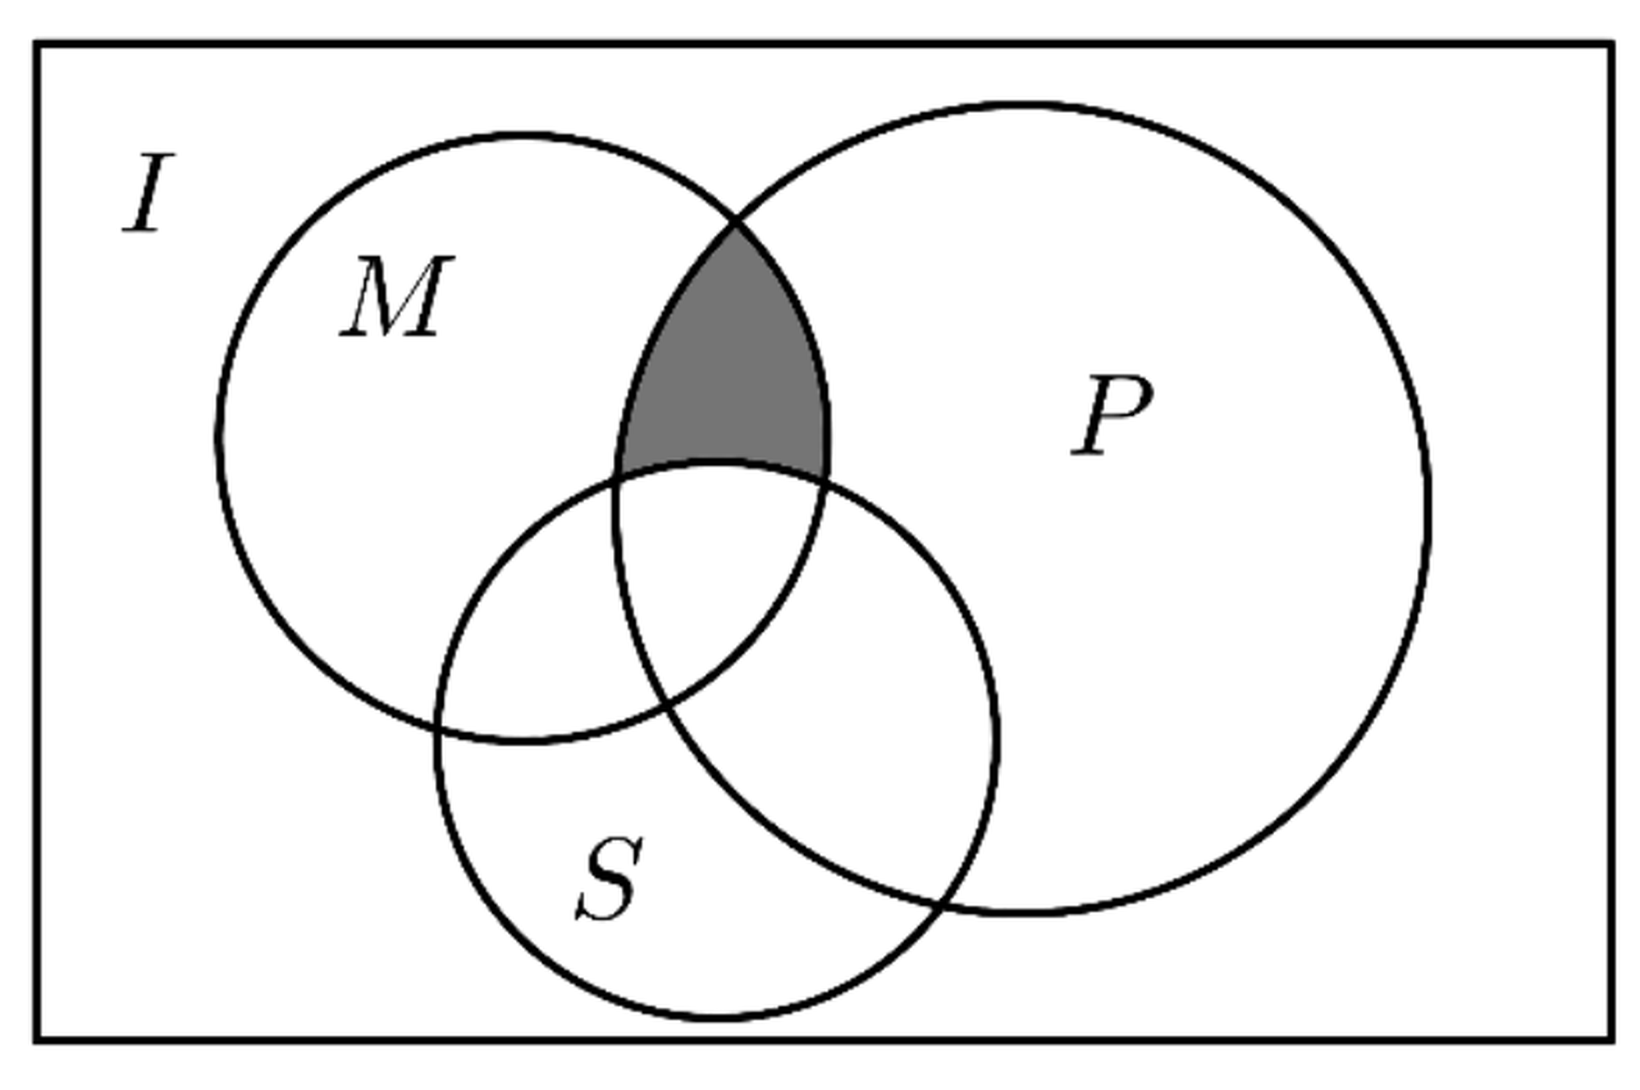
\includegraphics[width=0.42\textwidth]{figures/gao120_q15.png}
\end{center}

\keepwithprev
A. $(M\cap P)\cap S$\qquad\quad B. $(M\cap P)\cap\complement_{I}S$\qquad\quad C. $(M\cup P)\cap S$\qquad\quad D. $\complement_{I}(M\cap P)\cap S$

\ifanswer
\solbegin
\step{由已知中的 $Venn$ 图得阴影部分的元素属于 $M$，属于 $P$，但不属于 $S$，}
\step{所以阴影部分表示的集合为 $(M\cap P)\cap\complement_{I}S$，故选 $B$.}
\solend
\fi

\item 设集合 $P_1=\{x\mid x^2+ax+1>0\}$，$P_2=\{x\mid x^2+ax+2>0\}$，$Q_1=\{x\mid x^2+x+b>0\}$，$Q_2=\{x\mid x^2+2x+b>0\}$，其中 $a$、$b\in\R$，对于下列两个命题：①存在 $a$，$P_1$ 不是 $P_2$ 的子集；②存在 $b$ 使得 $Q_1$ 是 $Q_2$ 的子集. 下列说法正确的是\mbox{（\quad）}

\keepwithprev
A. ①是真命题，②是假命题\qquad\qquad B. ①是假命题，②是真命题

C. ①②都是真命题\qquad\qquad\qquad D. ①②都是假命题

\ifanswer
\solbegin
\step{对于集合 $P_1=\{x\mid x^2+ax+1>0\}$，$P_2=\{x\mid x^2+ax+2>0\}$，}
\step{得当 $m\in P_1$ 时，即 $m^2+am+1>0$，得 $m^2+am+2>0$，}
\step{即有 $m\in P_2$，得对任意 $a$，$P_1$ 是 $P_2$ 的子集，故①错误；}
\step{对于集合 $Q_1=\{x\mid x^2+x+b>0\}$，$Q_2=\{x\mid x^2+2x+b>0\}$，}
\step{当 $b=6$ 时，$Q_1=\{x\mid x^2+x+6>0\}=\R$，$Q_2=\{x\mid x^2+2x+6>0\}=\R$，}
\step{得 $Q_1$ 是 $Q_2$ 的子集，所以存在 $b$，使得 $Q_1$ 是 $Q_2$ 的子集，故②正确；}
\step{故选 $B$.}
\solend
\fi

\end{enumerate}

\bigsec{三、解答题}

\begin{enumerate}
\setcounter{enumi}{16}

\item (1) 已知 $x$、$y$ 都是实数，比较 $x^2+y^2$ 与 $4x-2y-5$ 的大小.

(2) 求解不等式组 $\begin{cases}x^2-4x+3\geqslant0\\\dfrac{x+3}{2x-1}\geqslant2\end{cases}$.

\ifanswer
\solbegin
\step{(1) $(x^2+y^2)-(4x-2y-5)=x^2-4x+y^2+2y+5=(x-2)^2+(y+1)^2\geqslant0$，}
\step{当 $x=2$，$y=-1$ 时，$x^2+y^2=4x-2y-5$.}
\step{当 $x\neq2$ 或 $y\neq-1$ 时，$x^2+y^2>4x-2y-5$.}
\step{(2) 由 $x^2-4x+3\geqslant0$ 得 $(x-1)(x-3)\geqslant0$，所以 $x\leqslant1$ 或 $x\geqslant3$；}
\step{由 $\dfrac{x+3}{2x-1}\geqslant2$，得 $\dfrac{x+3}{2x-1}-2=\dfrac{-3x+5}{2x-1}\geqslant0$，即 $\dfrac{3x-5}{2x-1}\leqslant0$，}
\step{所以 $\begin{cases}(3x-5)(2x-1)\leqslant0\\2x-1\neq0\end{cases}$，解得 $\dfrac12<x\leqslant\dfrac53$，}
\step{所以不等式组的解集是 $\left\{x\,\middle\vert\,\dfrac12<x\leqslant1\right\}$.}
\solend
\fi

\item 已知 $x_1$,$x_2$ 是一元二次方程 $4kx^2-4kx+k+1=0$ 的两个实数根.

(1) 是否存在实数 $k$，$(2x_1-x_2)(x_1-2x_2)=-\dfrac32$ 成立？若存在，求出 $k$ 的值；若不存在，请说明理由.

(2) 求使 $\dfrac{x_1}{x_2}+\dfrac{x_2}{x_1}-2$ 的值为整数的实数 $k$ 的整数值.

\ifanswer
\solbegin
\step{(1) 因为 $x_1$,$x_2$ 是一元二次方程 $4kx^2-4kx+k+1=0$ 的两个实数根，}
\step{所以 $\begin{cases}k\neq0\\16k^2-16k(k+1)\geqslant0\end{cases}$，所以 $k<0$，}
\step{由根与系数的关系得 $x_1+x_2=1$，$x_1x_2=\dfrac{k+1}{4k}$，}
\step{所以 $(2x_1-x_2)(x_1-2x_2)=2(x_1+x_2)^2-9x_1x_2=2-9\times\dfrac{k+1}{4k}=-\dfrac32$，}
\step{解得 $k=\dfrac95$，而 $k<0$，故不存在实数 $k$ 使得 $(2x_1-x_2)(x_1-2x_2)=-\dfrac32$ 成立.}
\step{(2) 由根与系数的关系得 $\dfrac{x_1}{x_2}+\dfrac{x_2}{x_1}-2=\dfrac{(x_1+x_2)^2}{x_1x_2}-4=-\dfrac4{k+1}$，}
\step{因为 $-\dfrac4{k+1}$ 的值为整数，而 $k$ 为整数，所以 $k+1$ 只能取 $\pm1$、$\pm2$、$\pm4$，}
\step{又 $k<0$，所以整数 $k$ 的值为 $-2$ 或 $-3$ 或 $-5$.}
\solend
\fi

\item 2026 年，某市低空经济蓬勃发展，一家物流企业开通“无人机即时配送”服务，并设立配送站. 经市场调研，该站每日配送单量 $y$（单位：单）与每单配送费 $x$（单位：元）满足关系式 $y=4800-200x$（其中 $4<x<24$）. 已知配送站每日的固定成本为 $19200$ 元，每完成一单配送，需支付电费、耗材费、设备保养费等可变成本，每单可变成本为 $4$ 元.

(1) 若要保证配送站每日利润 $W$（单位：元）不为负数，求每单配送费 $x$ 的取值范围；（每日利润 $=$ 每日配送总收入 $-$ 每日可变总成本 $-$ 每日固定成本）

(2) 为提升运力，该站购进一批新型无人机，购机费用为 $32$ 万元. 投入使用后，这批无人机使用 $t(t>0)$ 年的累计维保总费用为 $(2t^2+8t)$ 万元. 请问：这批无人机使用多少年后更新，可以使年平均总费用最低？请求出最低年平均总费用.（年平均总费用 $=$（购机费用 $+$ 维保总费用）$\div$ 使用年数）

\ifanswer
\solbegin
\step{(1) $W=xy-4y-19200=x(4800-200x)-4(4800-200x)-19200$}
\step{$=-200x^2+5600x-38400(4<x<24)$，}
\step{令 $W=-200x^2+5600x-38400\geqslant0$，即 $x^2-28x+192\leqslant0$，}
\step{解得 $12\leqslant x\leqslant16$，因此，要保证配送站每日利润 $W$ 不为负数，}
\step{每单配送费 $x$ 的取值范围为 $[12,16]$；}
\step{(2) 由题意，年平均总费用为 $N=\dfrac{2t^2+8t+32}{t}=2t+\dfrac{32}{t}+8$}
\step{$\geqslant2\sqrt{2t\cdot\dfrac{32}{t}}+8=16+8=24$，当且仅当 $2t=\dfrac{32}{t}$，即 $t=4$ 时取等号，}
\step{则这批无人机使用 $4$ 年后更新，可以使年平均总费用最低，}
\step{最低年平均总费用为 $24$ 万元.}
\solend
\fi

\item 已知 $A,B$，定义集合 $M_{(A,B)}=\{x\mid A<B\}$.

(1) 设 $A=\lvert x-4\rvert$,$B=2x$，求 $M_{(A,B)}$；

(2) 设 $A=ax^2+2ax-4$,$B=2x(x+2)$，当 $M_{(A,B)}=\R$ 时，求 $a$ 的取值范围；

(3) 设 $A=\lvert 2x-b\rvert$,$B=\dfrac{x+4b}{x-1}$,$C=2$，若 $M_{(A,C)}\cap M_{(B,C)}\neq\varnothing$，求 $b$ 的取值范围.

\ifanswer
\solbegin
\step{(1) 由定义，$x\in M_{(A,B)}$ 等价于 $\lvert x-4\rvert<2x$，}
\step{原不等式等价于 $-2x<x-4<2x$，即同时满足 $3x>4$ 与 $x>-4$，}
\step{解得 $x>\dfrac43$，所以 $M_{(A,B)}=\left(\dfrac43,+\infty\right)$.}
\step{(2) 由 $M_{(A,B)}=\R$，得 $ax^2+2ax-4<2x(x+2)$ 对任意 $x\in\R$ 恒成立，}
\step{得 $(a-2)(x+1)^2-a-2<0$.}
\step{当 $a>2$ 时，随着 $(x+1)^2$ 增大，左边可取正值，不符合题意；}
\step{当 $a=2$ 时，左边恒等于 $-4$，符合题意；}
\step{当 $a<2$ 时，左边在 $x=-1$ 处取得最大值 $-a-2$，}
\step{故恒成立的充要条件为 $-a-2<0$，即 $a>-2$；}
\step{综上，$a\in(-2,2]$.}
\step{(3) 由 $\lvert 2x-b\rvert<2$，得 $M_{(A,C)}=\left(\dfrac b2-1,\dfrac b2+1\right)$，记为 $I$.}
\step{由 $\dfrac{x+4b}{x-1}<2$，得 $\dfrac{x-(4b+2)}{x-1}>0$，其中 $x\neq1$.}
\step{①当 $b<-\dfrac14$ 时，$4b+2<1$，故 $M_{(B,C)}=(-\infty,4b+2)\cup(1,+\infty)$.}
\step{此时 $\dfrac b2+1<1$，所以 $I$ 与 $(1,+\infty)$ 没有公共元素.}
\step{两集合交集非空等价于 $\dfrac b2-1<4b+2$，解得 $b>-\dfrac67$.}
\step{因而本种情况得到 $-\dfrac67<b<-\dfrac14$.}
\step{②当 $b=-\dfrac14$ 时，$\dfrac{x+4b}{x-1}=1$，其中 $x\neq1$，故 $M_{(B,C)}=\{x\mid x\neq1\}$.}
\step{此时 $I=\left(-\dfrac98,\dfrac78\right)$，两集合交集非空.}
\step{③当 $b>-\dfrac14$ 时，$4b+2>1$，故 $M_{(B,C)}=(-\infty,1)\cup(4b+2,+\infty)$.}
\step{此时 $4b+2-\left(\dfrac b2+1\right)=\dfrac{7b}{2}+1>\dfrac18>0$，}
\step{所以 $I$ 与 $(4b+2,+\infty)$ 没有公共元素.}
\step{两集合交集非空等价于 $\dfrac b2-1<1$，解得 $b<4$.}
\step{因而本种情况得到 $-\dfrac14<b<4$.}
\step{综上，$b\in\left(-\dfrac67,4\right)$.}
\solend
\fi

\item 破晓同学阅读课外书籍时，发现笛卡尔积是代数和图论中一个很重要的课题. 对于非空数集 $A,B$，定义 $A\otimes B=\{(x,y)\mid x\in A$ 且 $y\in B\}$，将 $A\otimes B$ 称为“$A$ 与 $B$ 的笛卡尔积”.

(1) 若 $A=\{-1,0,1\}$,$B=\{-1,1\}$，求 $A\otimes B$ 和 $B\otimes A$；

(2) 试证明：“$A_1\otimes A_2=A_2\otimes A_1$”是“$A_1=A_2$”的充要条件；

(3) 若集合 $H$ 是有限集，将集合 $H$ 的元素个数记为 $\lvert H\rvert$. 已知 $\lvert A_1\otimes A_2\rvert=m^3(m\in\N^*)$，且存在实数 $a$ 满足 $\sqrt{\dfrac{\lvert A_1\otimes A_1\rvert+\lvert A_2\otimes A_2\rvert}{\lvert A_2\otimes A_1\rvert}}\geqslant a$ 对任意 $m\in\N^*$ 恒成立. 求 $a$ 的取值范围，并指明当 $a$ 取到最值时 $\lvert A_1\rvert$ 和 $\lvert A_2\rvert$ 满足的关系式及 $m$ 应满足的条件.

\ifanswer
\solbegin
\step{(1) 由题意得 $A\otimes B=\{(-1,-1),(-1,1),(0,-1),(0,1),(1,-1),(1,1)\}$，}
\step{$B\otimes A=\{(-1,-1),(-1,0),(-1,1),(1,-1),(1,0),(1,1)\}$；}
\step{(2) 若 $A_1=A_2$，设 $A_1=A_2=A$，}
\step{由定义得 $A_1\otimes A_2=\{(a,b)\mid a\in A$ 且 $b\in A\}=A_2\otimes A_1$，}
\step{所以“$A_1\otimes A_2=A_2\otimes A_1$”是“$A_1=A_2$”的必要条件；}
\step{若 $A_1\otimes A_2=A_2\otimes A_1$，对任意 $(a,b)\in A_1\otimes A_2$，均有 $(a,b)\in A_2\otimes A_1$，}
\step{即对任意 $a\in A_1,b\in A_2$，均有 $a\in A_2,b\in A_1$，}
\step{由任意性得 $A_1\subseteq A_2,A_2\subseteq A_1$，则 $A_1=A_2$，}
\step{所以“$A_1\otimes A_2=A_2\otimes A_1$”是“$A_1=A_2$”的充分条件；}
\step{综上所述，“$A_1\otimes A_2=A_2\otimes A_1$”是“$A_1=A_2$”的充要条件.}
\step{(3) 设 $\lvert A_1\rvert=c$,$\lvert A_2\rvert=d$,$c,d\in\N^*$，}
\step{则 $\lvert A_1\otimes A_2\rvert=\lvert A_2\otimes A_1\rvert=cd=m^3$,$\lvert A_1\otimes A_1\rvert=c^2$,$\lvert A_2\otimes A_2\rvert=d^2$，}
\step{得 $\sqrt{\dfrac{\lvert A_1\otimes A_1\rvert+\lvert A_2\otimes A_2\rvert}{\lvert A_2\otimes A_1\rvert}}=\sqrt{\dfrac{c^2+d^2}{cd}}=\sqrt{\dfrac cd+\dfrac dc}\geqslant\sqrt{2\sqrt{\dfrac cd\cdot\dfrac dc}}=\sqrt2$，}
\step{当且仅当 $\dfrac cd=\dfrac dc$，即 $c=d$ 时取等号，所以实数 $a$ 的取值范围是 $(-\infty,\sqrt2]$.}
\step{若 $a$ 取到最大值，则 $c=d$，即 $\lvert A_1\rvert=\lvert A_2\rvert$，得 $c^2=m^3$，}
\step{即 $c=\sqrt{m^3}=(\sqrt m)^3\in\N^*$，所以 $m=k^2,k\in\N^*$.}
\solend
\fi

\end{enumerate}

\end{document}
"
% 紧凑版：xelatex "\def\iscompact{1}% 高一120_松江二中_10月月考.tex
%   —— 高一上数学“2026-2027 年松江二中高一上 10 月月考”（试卷版/答案版）
% 试卷版：xelatex 高一120_松江二中_10月月考.tex
% 答案版：xelatex "\def\isanswer{1}% 高一120_松江二中_10月月考.tex
%   —— 高一上数学“2026-2027 年松江二中高一上 10 月月考”（试卷版/答案版）
% 试卷版：xelatex 高一120_松江二中_10月月考.tex
% 答案版：xelatex "\def\isanswer{1}\input{高一120_松江二中_10月月考.tex}"
% 紧凑版：xelatex "\def\iscompact{1}\input{高一120_松江二中_10月月考.tex}"
%
% 原始材料：微信公众号“魔都数学加油站”文章，作者破晓，2026-11-08 21:35 发布；
% 连载“27学年高一120”，原文标题“27学年高一120——2026-2027年上海市松江二中高一上10月月考”；
% 原文链接：https://mp.weixin.qq.com/s/hgDkaZX9M_IKhmr7CjQc1A。
% 正文为 10 张 PNG 页（第 8、10 页 2560×3620，其余 4762×6735），
% 题目下印有【解析】或【答案】，为讲评版。
% 题目、解析均据原图转录；卷面红色水印及公众号页脚未录入。
% 全卷 1 张插图：第 15 题的三集合 Venn 图（原卷印在题干右侧，本稿移至题干之后，
% 取原卷截图 2× LANCZOS 放大，见 figures/gao120_q15.png）。
%
% 卷首标题：原卷印作“2026-2027 年松江二中高一上 10 月月考”（公众号标题中的“上海市”
% 卷面标题行没有，本稿照卷面），年份区间按全稿惯例排 en dash；原卷未印副标题，本稿按题目内容
% 标为“集合与常用逻辑用语、不等式”（与 110／111／113／116／118 同）。
%
% 与原卷的排版差异：
%   ① 原文从第 3 题起，填空题编号为 3—12、选择题为 13—16、解答题为 17—21，本稿保留原题号；
%   ② 原卷每题下直接印【解析】／【答案】，本稿按全稿惯例置于答案版；第 3 题只印【答案】、
%      第 13、14 题把答案印在题干括号内且无【解析】，均另提 \ans{}；其余选择题答案在
%      解析末句“故选 …”，括号内留空；
%   ③ 原卷未印副标题，本稿按“知识模块”口径补出；
%   ④ 原卷填空横线按全稿惯例排为 \blankline[4.4em]；选择题括号排 \mbox{（\quad）}、
%      选项段前按惯例加 \keepwithprev；解答题不留作答区（原卷为讲评版，与 109—119 同）；
%   ⑤ 原卷数集排斜体 $R$、$N^*$，按全稿惯例改 \R、\N^*；绝对值排 \lvert…\rvert，
%      集合描述竖线排 \mid；补集记号照原卷排 \complement_I。
%
% 判别式字形：第 9 题解析作 $\triangle$（等边、扁），照录 \triangle。
%
% 子集符号：第 4 题题干与解析的 $A\subseteq B$、第 21 题 (2) 的 $A_1\subseteq A_2$ 印有下划线，
%   照录 \subseteq。
%
% 原卷存疑照录：第 12 题题干 $S=\{82,83,84,85,86,87,89\}$ 跳过 $88$ 只列 7 个数，
%   与其“8 种不同的值”自洽（不含 $88$），照录；第 19 题 (1) 的 $W$ 表达式
%   $x(4800-200x)-4(4800-200x)-19200$ 与最后结果 $[12,16]$ 一致。
%
% 行数核对：逐题数 \step 条数，合计 115 条（Q3：0；Q4：4；Q5：2；Q6：5；Q7：4；
% Q8：2；Q9：5；Q10：3；Q11：6；Q12：11；Q13：0；Q14：0；Q15：2；Q16：7；
% Q17：7；Q18：8；Q19：9；Q20：24；Q21：16），与原卷印刷行逐题相等
% （cases 块作一个印刷行计）。第 3 题只印【答案】、第 13、14 题括号内印答案且无解析，
% 均提 \ans{}，不计入 \step 账。
%
\documentclass[a4paper,11pt]{article}
\usepackage{common}

\begin{document}

\examtitlest[3]{2026--2027 年松江二中高一上 10 月月考}{集合与常用逻辑用语、不等式}

\bigsec{一、填空题}

\begin{enumerate}
\setcounter{enumi}{2}

\item 集合 $A=\{(x,y)\mid x+y=8\}$,$B=\{(x,y)\mid xy=12\}$，求 $A\cap B=$\blankline[4.4em].

\ifanswer
\ans{$\{(2,6),(6,2)\}$}
\fi

\item 设集合 $A=\{0,-a\}$,$B=\{1,a-2,2a-2\}$，若 $A\subseteq B$，则 $a=$\blankline[4.4em].

\ifanswer
\solbegin
\step{因为 $A\subseteq B$，}
\step{若 $a-2=0$，解得 $a=2$，此时 $A=\{0,-2\}$,$B=\{1,0,2\}$，不符合题意；}
\step{若 $2a-2=0$，解得 $a=1$，此时 $A=\{0,-1\}$,$B=\{1,-1,0\}$，符合题意；}
\step{综上所述，$a=1$.}
\solend
\fi

\item 设 $\alpha:0<x<a(a>0)$,$\beta:x<8-3a$，若 $\alpha$ 是 $\beta$ 的充分条件，则实数 $a$ 的取值范围是\blankline[4.4em].

\ifanswer
\solbegin
\step{由 $\alpha$ 是 $\beta$ 的充分条件得，$x\in(0,a)\Rightarrow x\in(-\infty,8-3a)$，}
\step{所以 $0<a\leqslant8-3a$，解得 $0<a\leqslant2$.}
\solend
\fi

\item 关于 $x$ 的不等式 $ax-b>0$ 的解集为 $(-\infty,1)$，则不等式 $\dfrac{x-2}{ax+b}<0$ 的解集为\blankline[4.4em].

\ifanswer
\solbegin
\step{因为关于 $x$ 的不等式 $ax-b>0$ 的解集为 $(-\infty,1)$，}
\step{所以 $a<0$ 且 $\dfrac ba=1$，则 $b=a$，}
\step{所以不等式 $\dfrac{x-2}{ax+b}<0$，即 $\dfrac{x-2}{ax+a}<0$，即 $\dfrac{x-2}{x+1}>0$，}
\step{等价于 $(x+1)(x-2)>0$，解得 $x>2$ 或 $x<-1$，}
\step{即解集为 $(-\infty,-1)\cup(2,+\infty)$.}
\solend
\fi

\item 若正实数 $x$、$y$ 满足 $2x+y+8xy=2$，则 $xy$ 的最大值为\blankline[4.4em].

\ifanswer
\solbegin
\step{因为正实数 $x$、$y$ 满足 $2x+y+8xy=2$，}
\step{所以 $2-8xy=2x+y\geqslant2\sqrt{2xy}$，}
\step{当且仅当 $y=2x$，即 $x=\dfrac14$，$y=\dfrac12$ 时取等号，解得 $0<xy\leqslant\dfrac18$，}
\step{故 $xy$ 的最大值为 $\dfrac18$.}
\solend
\fi

\item 已知 $1<a<3$，$-5<b<-2$，则 $\dfrac ab$ 的取值范围是\blankline[4.4em].

\ifanswer
\solbegin
\step{因为 $-5<b<-2$，所以 $2<-b<5$，$\dfrac15<-\dfrac1b<\dfrac12$，又 $1<a<3$，}
\step{得 $\dfrac15<-\dfrac ab<\dfrac32$，则 $-\dfrac32<\dfrac ab<-\dfrac15$，故 $\dfrac ab$ 的取值范围是 $\left(-\dfrac32,-\dfrac15\right)$.}
\solend
\fi

\item 若关于 $x$、$y$ 的方程组 $\begin{cases}y-kx-2=0\\y^2-4x-2y+1=0\end{cases}$ 的解集中只有一个元素，则实数 $k$ 的值为\blankline[4.4em].

\ifanswer
\solbegin
\step{由 $\begin{cases}y-kx-2=0\\y^2-4x-2y+1=0\end{cases}$ 消去 $y$ 整理得 $k^2x^2+(2k-4)x+1=0$.}
\step{当 $k\neq0$ 时，则 $\triangle=(2k-4)^2-4k^2=0$，解得 $k=1$，}
\step{此时方程组的解为 $\begin{cases}x=1\\y=3\end{cases}$，符合题意；}
\step{当 $k=0$ 时，解得 $x=\dfrac14$，此时方程组的解为 $\begin{cases}x=\dfrac14\\y=2\end{cases}$，符合题意；}
\step{综上，$k=0$ 或 $k=1$.}
\solend
\fi

\item 若集合 $A=\{0,1\}$，$B=\{x\mid x^2-mx-m>0,x\in\R\}$，且 $A\cap B=\{1\}$，则实数 $m$ 的取值范围为\blankline[4.4em].

\ifanswer
\solbegin
\step{因为集合 $A=\{0,1\}$，$B=\{x\mid x^2-mx-m>0,x\in\R\}$，且 $A\cap B=\{1\}$，}
\step{则 $1\in B$ 且 $0\notin B$，所以 $\begin{cases}1-m-m>0\\-m\leqslant0\end{cases}$，解得 $0\leqslant m<\dfrac12$，}
\step{所以实数 $m$ 的取值范围是 $\left[0,\dfrac12\right)$.}
\solend
\fi

\item 从集合 $U=\{a,b,c,d\}$ 的子集中选出两个不同的子集，需同时满足以下两个条件：(1) $a$、$b$ 都至少属于其中一个集合；(2) 对选出的两个子集，其中一个集合为另一个的子集，那么共有\blankline[4.4em]种不同的选法.

\ifanswer
\solbegin
\step{不妨设元素少的为 $A$，元素多的为 $B$，则 $B$ 必包含有 $a$、$b$；$A$ 为 $B$ 的真子集，}
\step{若 $B=\{a,b\}$，$A$ 为 $B$ 的真子集，共 $2^2-1=3$ 种，}
\step{若 $B=\{a,b,c\}$，$A$ 为 $B$ 的真子集，共 $2^3-1=7$ 种，}
\step{若 $B=\{a,b,d\}$，$A$ 为 $B$ 的真子集，共 $2^3-1=7$ 种，}
\step{若 $B=\{a,b,c,d\}$，$A$ 为 $B$ 的真子集，共 $2^4-1=15$ 种，}
\step{共有 $3+7+7+15=32$ 种.}
\solend
\fi

\item 已知 $a_1$、$a_2$、$\cdots$、$a_8$ 是 $8$ 个正整数，记 $S=\{a_{i_1}+a_{i_2}+\cdots+a_{i_7}\mid 1\leqslant i_1<i_2<\cdots<i_7\leqslant8\}$，其中 $i_1$、$i_2$、$\cdots$、$i_7\in\N^*$，若 $S=\{82,83,84,85,86,87,89\}$，则这 $8$ 个正整数中的最大数与最小数的积为\blankline[4.4em].

\ifanswer
\solbegin
\step{由题意得从 $8$ 个数中任取 $7$ 个数的和共有 $C_8^7=8$ 种不同的值，}
\step{但是 $82$，$83$，$84$，$85$，$86$，$87$，$89$ 只有 $7$ 个数，}
\step{得必有两种 $7$ 个数的和相等，设这个和为 $t(82\leqslant t\leqslant89)$，}
\step{令 $T=\sum\limits_{i=1}^{8}a_i$，那么，任取 $7$ 个数的和就等于 $T-a_i$，$i=1,2,\cdots,8$，}
\step{这 $8$ 个取值和的集合为 $S$，$S=\{T-a_1,T-a_2,\cdots,T-a_8\}$，}
\step{则 $\sum\limits_{i=1}^{8}(T-a_i)=8T-T=7T=82+83+84+85+86+87+89+t=596+t$.}
\step{因为 $T$ 为整数，所以 $596+t$ 是 $7$ 的倍数，}
\step{由 $596=7\times85+1$ 得 $1+t$ 是 $7$ 的倍数，}
\step{再因为 $82\leqslant t\leqslant89$，所以 $t=83$，得 $T=97$.}
\step{因此 $a_1$、$a_2$、$\cdots$、$a_8$ 中最大数为 $97-82=15$，最小数为 $97-89=8$，}
\step{因此，它们的积为 $120$.}
\solend
\fi

\end{enumerate}

\bigsec{二、选择题}

\begin{enumerate}
\setcounter{enumi}{12}

\item 已知 $a>b>0$，$c\in\R$，则下列不等式不一定成立的是\mbox{（\quad）}% 原卷把答案“$B$”印在题干括号内、无【解析】

\keepwithprev
A. $a-c>b-c$\qquad\quad B. $ac>bc$\qquad\quad C. $\dfrac1a<\dfrac1b$\qquad\quad D. $\dfrac{a+b}{2}>\sqrt{ab}$

\ifanswer
\ans{$B$}
\fi

\item 命题“对任意的 $x\in\R,x^3-x^2+1\leqslant0$”的否定是\mbox{（\quad）}% 原卷把答案“$C$”印在题干括号内、无【解析】

\keepwithprev
A. 不存在 $x\in\R,x^3-x^2+1\leqslant0$\qquad B. 存在 $x\in\R,x^3-x^2+1\leqslant0$

C. 存在 $x\in\R,x^3-x^2+1>0$\qquad\quad D. 对任意的 $x\in\R,x^3-x^2+1>0$

\ifanswer
\ans{$C$}
\fi

% 第 15 题是“题干 + 图 + 选项”约 6.5cm 的一整块，\keepwithprev 只挡得住“图—选项”，
% 挡不住夹在中间的图——实测断点落在题干之后（切页审计 A 类）。故照 高一30／高一26 成例
% 在题前先量一次页高，不够就把整块一起挪到次页。
\needvspace{7cm}
\item 如图，$I$ 是全集，$M$、$P$、$S$ 是 $I$ 的三个子集，则阴影部分所表示的集合是\mbox{（\quad）}

\begin{center}
% 图取原卷截图（第 4 页题干右侧）、2× LANCZOS 放大，本稿移至题干之后
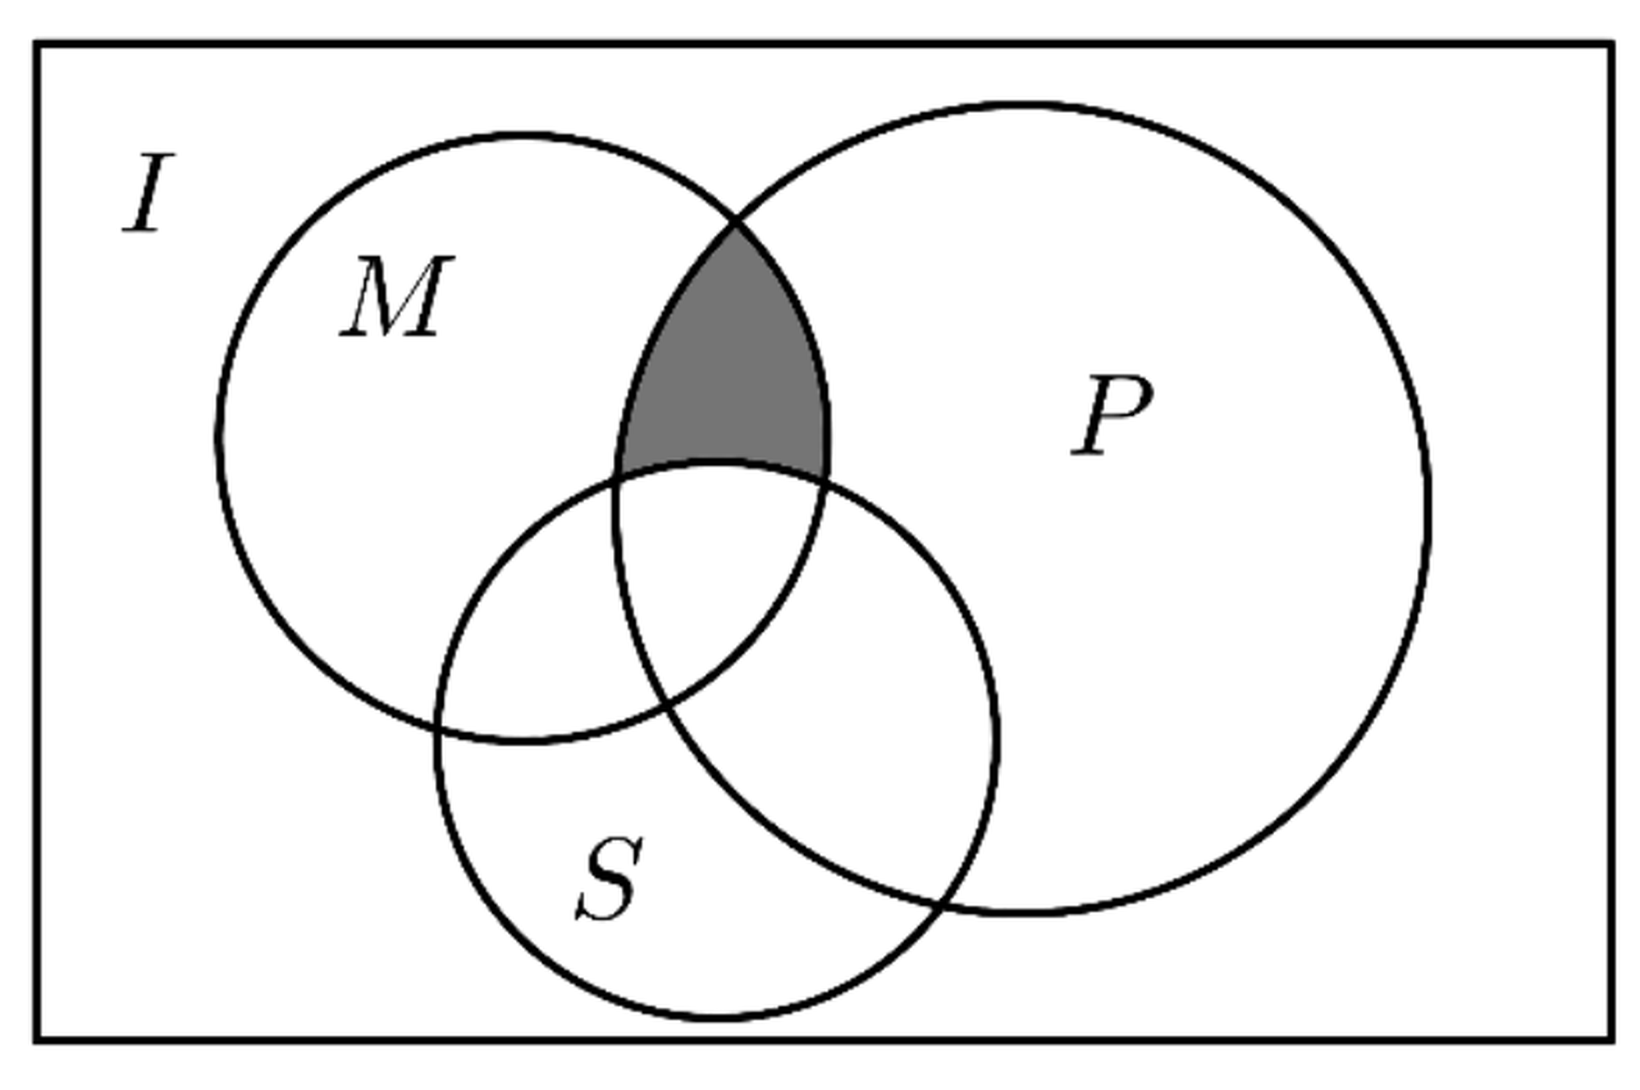
\includegraphics[width=0.42\textwidth]{figures/gao120_q15.png}
\end{center}

\keepwithprev
A. $(M\cap P)\cap S$\qquad\quad B. $(M\cap P)\cap\complement_{I}S$\qquad\quad C. $(M\cup P)\cap S$\qquad\quad D. $\complement_{I}(M\cap P)\cap S$

\ifanswer
\solbegin
\step{由已知中的 $Venn$ 图得阴影部分的元素属于 $M$，属于 $P$，但不属于 $S$，}
\step{所以阴影部分表示的集合为 $(M\cap P)\cap\complement_{I}S$，故选 $B$.}
\solend
\fi

\item 设集合 $P_1=\{x\mid x^2+ax+1>0\}$，$P_2=\{x\mid x^2+ax+2>0\}$，$Q_1=\{x\mid x^2+x+b>0\}$，$Q_2=\{x\mid x^2+2x+b>0\}$，其中 $a$、$b\in\R$，对于下列两个命题：①存在 $a$，$P_1$ 不是 $P_2$ 的子集；②存在 $b$ 使得 $Q_1$ 是 $Q_2$ 的子集. 下列说法正确的是\mbox{（\quad）}

\keepwithprev
A. ①是真命题，②是假命题\qquad\qquad B. ①是假命题，②是真命题

C. ①②都是真命题\qquad\qquad\qquad D. ①②都是假命题

\ifanswer
\solbegin
\step{对于集合 $P_1=\{x\mid x^2+ax+1>0\}$，$P_2=\{x\mid x^2+ax+2>0\}$，}
\step{得当 $m\in P_1$ 时，即 $m^2+am+1>0$，得 $m^2+am+2>0$，}
\step{即有 $m\in P_2$，得对任意 $a$，$P_1$ 是 $P_2$ 的子集，故①错误；}
\step{对于集合 $Q_1=\{x\mid x^2+x+b>0\}$，$Q_2=\{x\mid x^2+2x+b>0\}$，}
\step{当 $b=6$ 时，$Q_1=\{x\mid x^2+x+6>0\}=\R$，$Q_2=\{x\mid x^2+2x+6>0\}=\R$，}
\step{得 $Q_1$ 是 $Q_2$ 的子集，所以存在 $b$，使得 $Q_1$ 是 $Q_2$ 的子集，故②正确；}
\step{故选 $B$.}
\solend
\fi

\end{enumerate}

\bigsec{三、解答题}

\begin{enumerate}
\setcounter{enumi}{16}

\item (1) 已知 $x$、$y$ 都是实数，比较 $x^2+y^2$ 与 $4x-2y-5$ 的大小.

(2) 求解不等式组 $\begin{cases}x^2-4x+3\geqslant0\\\dfrac{x+3}{2x-1}\geqslant2\end{cases}$.

\ifanswer
\solbegin
\step{(1) $(x^2+y^2)-(4x-2y-5)=x^2-4x+y^2+2y+5=(x-2)^2+(y+1)^2\geqslant0$，}
\step{当 $x=2$，$y=-1$ 时，$x^2+y^2=4x-2y-5$.}
\step{当 $x\neq2$ 或 $y\neq-1$ 时，$x^2+y^2>4x-2y-5$.}
\step{(2) 由 $x^2-4x+3\geqslant0$ 得 $(x-1)(x-3)\geqslant0$，所以 $x\leqslant1$ 或 $x\geqslant3$；}
\step{由 $\dfrac{x+3}{2x-1}\geqslant2$，得 $\dfrac{x+3}{2x-1}-2=\dfrac{-3x+5}{2x-1}\geqslant0$，即 $\dfrac{3x-5}{2x-1}\leqslant0$，}
\step{所以 $\begin{cases}(3x-5)(2x-1)\leqslant0\\2x-1\neq0\end{cases}$，解得 $\dfrac12<x\leqslant\dfrac53$，}
\step{所以不等式组的解集是 $\left\{x\,\middle\vert\,\dfrac12<x\leqslant1\right\}$.}
\solend
\fi

\item 已知 $x_1$,$x_2$ 是一元二次方程 $4kx^2-4kx+k+1=0$ 的两个实数根.

(1) 是否存在实数 $k$，$(2x_1-x_2)(x_1-2x_2)=-\dfrac32$ 成立？若存在，求出 $k$ 的值；若不存在，请说明理由.

(2) 求使 $\dfrac{x_1}{x_2}+\dfrac{x_2}{x_1}-2$ 的值为整数的实数 $k$ 的整数值.

\ifanswer
\solbegin
\step{(1) 因为 $x_1$,$x_2$ 是一元二次方程 $4kx^2-4kx+k+1=0$ 的两个实数根，}
\step{所以 $\begin{cases}k\neq0\\16k^2-16k(k+1)\geqslant0\end{cases}$，所以 $k<0$，}
\step{由根与系数的关系得 $x_1+x_2=1$，$x_1x_2=\dfrac{k+1}{4k}$，}
\step{所以 $(2x_1-x_2)(x_1-2x_2)=2(x_1+x_2)^2-9x_1x_2=2-9\times\dfrac{k+1}{4k}=-\dfrac32$，}
\step{解得 $k=\dfrac95$，而 $k<0$，故不存在实数 $k$ 使得 $(2x_1-x_2)(x_1-2x_2)=-\dfrac32$ 成立.}
\step{(2) 由根与系数的关系得 $\dfrac{x_1}{x_2}+\dfrac{x_2}{x_1}-2=\dfrac{(x_1+x_2)^2}{x_1x_2}-4=-\dfrac4{k+1}$，}
\step{因为 $-\dfrac4{k+1}$ 的值为整数，而 $k$ 为整数，所以 $k+1$ 只能取 $\pm1$、$\pm2$、$\pm4$，}
\step{又 $k<0$，所以整数 $k$ 的值为 $-2$ 或 $-3$ 或 $-5$.}
\solend
\fi

\item 2026 年，某市低空经济蓬勃发展，一家物流企业开通“无人机即时配送”服务，并设立配送站. 经市场调研，该站每日配送单量 $y$（单位：单）与每单配送费 $x$（单位：元）满足关系式 $y=4800-200x$（其中 $4<x<24$）. 已知配送站每日的固定成本为 $19200$ 元，每完成一单配送，需支付电费、耗材费、设备保养费等可变成本，每单可变成本为 $4$ 元.

(1) 若要保证配送站每日利润 $W$（单位：元）不为负数，求每单配送费 $x$ 的取值范围；（每日利润 $=$ 每日配送总收入 $-$ 每日可变总成本 $-$ 每日固定成本）

(2) 为提升运力，该站购进一批新型无人机，购机费用为 $32$ 万元. 投入使用后，这批无人机使用 $t(t>0)$ 年的累计维保总费用为 $(2t^2+8t)$ 万元. 请问：这批无人机使用多少年后更新，可以使年平均总费用最低？请求出最低年平均总费用.（年平均总费用 $=$（购机费用 $+$ 维保总费用）$\div$ 使用年数）

\ifanswer
\solbegin
\step{(1) $W=xy-4y-19200=x(4800-200x)-4(4800-200x)-19200$}
\step{$=-200x^2+5600x-38400(4<x<24)$，}
\step{令 $W=-200x^2+5600x-38400\geqslant0$，即 $x^2-28x+192\leqslant0$，}
\step{解得 $12\leqslant x\leqslant16$，因此，要保证配送站每日利润 $W$ 不为负数，}
\step{每单配送费 $x$ 的取值范围为 $[12,16]$；}
\step{(2) 由题意，年平均总费用为 $N=\dfrac{2t^2+8t+32}{t}=2t+\dfrac{32}{t}+8$}
\step{$\geqslant2\sqrt{2t\cdot\dfrac{32}{t}}+8=16+8=24$，当且仅当 $2t=\dfrac{32}{t}$，即 $t=4$ 时取等号，}
\step{则这批无人机使用 $4$ 年后更新，可以使年平均总费用最低，}
\step{最低年平均总费用为 $24$ 万元.}
\solend
\fi

\item 已知 $A,B$，定义集合 $M_{(A,B)}=\{x\mid A<B\}$.

(1) 设 $A=\lvert x-4\rvert$,$B=2x$，求 $M_{(A,B)}$；

(2) 设 $A=ax^2+2ax-4$,$B=2x(x+2)$，当 $M_{(A,B)}=\R$ 时，求 $a$ 的取值范围；

(3) 设 $A=\lvert 2x-b\rvert$,$B=\dfrac{x+4b}{x-1}$,$C=2$，若 $M_{(A,C)}\cap M_{(B,C)}\neq\varnothing$，求 $b$ 的取值范围.

\ifanswer
\solbegin
\step{(1) 由定义，$x\in M_{(A,B)}$ 等价于 $\lvert x-4\rvert<2x$，}
\step{原不等式等价于 $-2x<x-4<2x$，即同时满足 $3x>4$ 与 $x>-4$，}
\step{解得 $x>\dfrac43$，所以 $M_{(A,B)}=\left(\dfrac43,+\infty\right)$.}
\step{(2) 由 $M_{(A,B)}=\R$，得 $ax^2+2ax-4<2x(x+2)$ 对任意 $x\in\R$ 恒成立，}
\step{得 $(a-2)(x+1)^2-a-2<0$.}
\step{当 $a>2$ 时，随着 $(x+1)^2$ 增大，左边可取正值，不符合题意；}
\step{当 $a=2$ 时，左边恒等于 $-4$，符合题意；}
\step{当 $a<2$ 时，左边在 $x=-1$ 处取得最大值 $-a-2$，}
\step{故恒成立的充要条件为 $-a-2<0$，即 $a>-2$；}
\step{综上，$a\in(-2,2]$.}
\step{(3) 由 $\lvert 2x-b\rvert<2$，得 $M_{(A,C)}=\left(\dfrac b2-1,\dfrac b2+1\right)$，记为 $I$.}
\step{由 $\dfrac{x+4b}{x-1}<2$，得 $\dfrac{x-(4b+2)}{x-1}>0$，其中 $x\neq1$.}
\step{①当 $b<-\dfrac14$ 时，$4b+2<1$，故 $M_{(B,C)}=(-\infty,4b+2)\cup(1,+\infty)$.}
\step{此时 $\dfrac b2+1<1$，所以 $I$ 与 $(1,+\infty)$ 没有公共元素.}
\step{两集合交集非空等价于 $\dfrac b2-1<4b+2$，解得 $b>-\dfrac67$.}
\step{因而本种情况得到 $-\dfrac67<b<-\dfrac14$.}
\step{②当 $b=-\dfrac14$ 时，$\dfrac{x+4b}{x-1}=1$，其中 $x\neq1$，故 $M_{(B,C)}=\{x\mid x\neq1\}$.}
\step{此时 $I=\left(-\dfrac98,\dfrac78\right)$，两集合交集非空.}
\step{③当 $b>-\dfrac14$ 时，$4b+2>1$，故 $M_{(B,C)}=(-\infty,1)\cup(4b+2,+\infty)$.}
\step{此时 $4b+2-\left(\dfrac b2+1\right)=\dfrac{7b}{2}+1>\dfrac18>0$，}
\step{所以 $I$ 与 $(4b+2,+\infty)$ 没有公共元素.}
\step{两集合交集非空等价于 $\dfrac b2-1<1$，解得 $b<4$.}
\step{因而本种情况得到 $-\dfrac14<b<4$.}
\step{综上，$b\in\left(-\dfrac67,4\right)$.}
\solend
\fi

\item 破晓同学阅读课外书籍时，发现笛卡尔积是代数和图论中一个很重要的课题. 对于非空数集 $A,B$，定义 $A\otimes B=\{(x,y)\mid x\in A$ 且 $y\in B\}$，将 $A\otimes B$ 称为“$A$ 与 $B$ 的笛卡尔积”.

(1) 若 $A=\{-1,0,1\}$,$B=\{-1,1\}$，求 $A\otimes B$ 和 $B\otimes A$；

(2) 试证明：“$A_1\otimes A_2=A_2\otimes A_1$”是“$A_1=A_2$”的充要条件；

(3) 若集合 $H$ 是有限集，将集合 $H$ 的元素个数记为 $\lvert H\rvert$. 已知 $\lvert A_1\otimes A_2\rvert=m^3(m\in\N^*)$，且存在实数 $a$ 满足 $\sqrt{\dfrac{\lvert A_1\otimes A_1\rvert+\lvert A_2\otimes A_2\rvert}{\lvert A_2\otimes A_1\rvert}}\geqslant a$ 对任意 $m\in\N^*$ 恒成立. 求 $a$ 的取值范围，并指明当 $a$ 取到最值时 $\lvert A_1\rvert$ 和 $\lvert A_2\rvert$ 满足的关系式及 $m$ 应满足的条件.

\ifanswer
\solbegin
\step{(1) 由题意得 $A\otimes B=\{(-1,-1),(-1,1),(0,-1),(0,1),(1,-1),(1,1)\}$，}
\step{$B\otimes A=\{(-1,-1),(-1,0),(-1,1),(1,-1),(1,0),(1,1)\}$；}
\step{(2) 若 $A_1=A_2$，设 $A_1=A_2=A$，}
\step{由定义得 $A_1\otimes A_2=\{(a,b)\mid a\in A$ 且 $b\in A\}=A_2\otimes A_1$，}
\step{所以“$A_1\otimes A_2=A_2\otimes A_1$”是“$A_1=A_2$”的必要条件；}
\step{若 $A_1\otimes A_2=A_2\otimes A_1$，对任意 $(a,b)\in A_1\otimes A_2$，均有 $(a,b)\in A_2\otimes A_1$，}
\step{即对任意 $a\in A_1,b\in A_2$，均有 $a\in A_2,b\in A_1$，}
\step{由任意性得 $A_1\subseteq A_2,A_2\subseteq A_1$，则 $A_1=A_2$，}
\step{所以“$A_1\otimes A_2=A_2\otimes A_1$”是“$A_1=A_2$”的充分条件；}
\step{综上所述，“$A_1\otimes A_2=A_2\otimes A_1$”是“$A_1=A_2$”的充要条件.}
\step{(3) 设 $\lvert A_1\rvert=c$,$\lvert A_2\rvert=d$,$c,d\in\N^*$，}
\step{则 $\lvert A_1\otimes A_2\rvert=\lvert A_2\otimes A_1\rvert=cd=m^3$,$\lvert A_1\otimes A_1\rvert=c^2$,$\lvert A_2\otimes A_2\rvert=d^2$，}
\step{得 $\sqrt{\dfrac{\lvert A_1\otimes A_1\rvert+\lvert A_2\otimes A_2\rvert}{\lvert A_2\otimes A_1\rvert}}=\sqrt{\dfrac{c^2+d^2}{cd}}=\sqrt{\dfrac cd+\dfrac dc}\geqslant\sqrt{2\sqrt{\dfrac cd\cdot\dfrac dc}}=\sqrt2$，}
\step{当且仅当 $\dfrac cd=\dfrac dc$，即 $c=d$ 时取等号，所以实数 $a$ 的取值范围是 $(-\infty,\sqrt2]$.}
\step{若 $a$ 取到最大值，则 $c=d$，即 $\lvert A_1\rvert=\lvert A_2\rvert$，得 $c^2=m^3$，}
\step{即 $c=\sqrt{m^3}=(\sqrt m)^3\in\N^*$，所以 $m=k^2,k\in\N^*$.}
\solend
\fi

\end{enumerate}

\end{document}
"
% 紧凑版：xelatex "\def\iscompact{1}% 高一120_松江二中_10月月考.tex
%   —— 高一上数学“2026-2027 年松江二中高一上 10 月月考”（试卷版/答案版）
% 试卷版：xelatex 高一120_松江二中_10月月考.tex
% 答案版：xelatex "\def\isanswer{1}\input{高一120_松江二中_10月月考.tex}"
% 紧凑版：xelatex "\def\iscompact{1}\input{高一120_松江二中_10月月考.tex}"
%
% 原始材料：微信公众号“魔都数学加油站”文章，作者破晓，2026-11-08 21:35 发布；
% 连载“27学年高一120”，原文标题“27学年高一120——2026-2027年上海市松江二中高一上10月月考”；
% 原文链接：https://mp.weixin.qq.com/s/hgDkaZX9M_IKhmr7CjQc1A。
% 正文为 10 张 PNG 页（第 8、10 页 2560×3620，其余 4762×6735），
% 题目下印有【解析】或【答案】，为讲评版。
% 题目、解析均据原图转录；卷面红色水印及公众号页脚未录入。
% 全卷 1 张插图：第 15 题的三集合 Venn 图（原卷印在题干右侧，本稿移至题干之后，
% 取原卷截图 2× LANCZOS 放大，见 figures/gao120_q15.png）。
%
% 卷首标题：原卷印作“2026-2027 年松江二中高一上 10 月月考”（公众号标题中的“上海市”
% 卷面标题行没有，本稿照卷面），年份区间按全稿惯例排 en dash；原卷未印副标题，本稿按题目内容
% 标为“集合与常用逻辑用语、不等式”（与 110／111／113／116／118 同）。
%
% 与原卷的排版差异：
%   ① 原文从第 3 题起，填空题编号为 3—12、选择题为 13—16、解答题为 17—21，本稿保留原题号；
%   ② 原卷每题下直接印【解析】／【答案】，本稿按全稿惯例置于答案版；第 3 题只印【答案】、
%      第 13、14 题把答案印在题干括号内且无【解析】，均另提 \ans{}；其余选择题答案在
%      解析末句“故选 …”，括号内留空；
%   ③ 原卷未印副标题，本稿按“知识模块”口径补出；
%   ④ 原卷填空横线按全稿惯例排为 \blankline[4.4em]；选择题括号排 \mbox{（\quad）}、
%      选项段前按惯例加 \keepwithprev；解答题不留作答区（原卷为讲评版，与 109—119 同）；
%   ⑤ 原卷数集排斜体 $R$、$N^*$，按全稿惯例改 \R、\N^*；绝对值排 \lvert…\rvert，
%      集合描述竖线排 \mid；补集记号照原卷排 \complement_I。
%
% 判别式字形：第 9 题解析作 $\triangle$（等边、扁），照录 \triangle。
%
% 子集符号：第 4 题题干与解析的 $A\subseteq B$、第 21 题 (2) 的 $A_1\subseteq A_2$ 印有下划线，
%   照录 \subseteq。
%
% 原卷存疑照录：第 12 题题干 $S=\{82,83,84,85,86,87,89\}$ 跳过 $88$ 只列 7 个数，
%   与其“8 种不同的值”自洽（不含 $88$），照录；第 19 题 (1) 的 $W$ 表达式
%   $x(4800-200x)-4(4800-200x)-19200$ 与最后结果 $[12,16]$ 一致。
%
% 行数核对：逐题数 \step 条数，合计 115 条（Q3：0；Q4：4；Q5：2；Q6：5；Q7：4；
% Q8：2；Q9：5；Q10：3；Q11：6；Q12：11；Q13：0；Q14：0；Q15：2；Q16：7；
% Q17：7；Q18：8；Q19：9；Q20：24；Q21：16），与原卷印刷行逐题相等
% （cases 块作一个印刷行计）。第 3 题只印【答案】、第 13、14 题括号内印答案且无解析，
% 均提 \ans{}，不计入 \step 账。
%
\documentclass[a4paper,11pt]{article}
\usepackage{common}

\begin{document}

\examtitlest[3]{2026--2027 年松江二中高一上 10 月月考}{集合与常用逻辑用语、不等式}

\bigsec{一、填空题}

\begin{enumerate}
\setcounter{enumi}{2}

\item 集合 $A=\{(x,y)\mid x+y=8\}$,$B=\{(x,y)\mid xy=12\}$，求 $A\cap B=$\blankline[4.4em].

\ifanswer
\ans{$\{(2,6),(6,2)\}$}
\fi

\item 设集合 $A=\{0,-a\}$,$B=\{1,a-2,2a-2\}$，若 $A\subseteq B$，则 $a=$\blankline[4.4em].

\ifanswer
\solbegin
\step{因为 $A\subseteq B$，}
\step{若 $a-2=0$，解得 $a=2$，此时 $A=\{0,-2\}$,$B=\{1,0,2\}$，不符合题意；}
\step{若 $2a-2=0$，解得 $a=1$，此时 $A=\{0,-1\}$,$B=\{1,-1,0\}$，符合题意；}
\step{综上所述，$a=1$.}
\solend
\fi

\item 设 $\alpha:0<x<a(a>0)$,$\beta:x<8-3a$，若 $\alpha$ 是 $\beta$ 的充分条件，则实数 $a$ 的取值范围是\blankline[4.4em].

\ifanswer
\solbegin
\step{由 $\alpha$ 是 $\beta$ 的充分条件得，$x\in(0,a)\Rightarrow x\in(-\infty,8-3a)$，}
\step{所以 $0<a\leqslant8-3a$，解得 $0<a\leqslant2$.}
\solend
\fi

\item 关于 $x$ 的不等式 $ax-b>0$ 的解集为 $(-\infty,1)$，则不等式 $\dfrac{x-2}{ax+b}<0$ 的解集为\blankline[4.4em].

\ifanswer
\solbegin
\step{因为关于 $x$ 的不等式 $ax-b>0$ 的解集为 $(-\infty,1)$，}
\step{所以 $a<0$ 且 $\dfrac ba=1$，则 $b=a$，}
\step{所以不等式 $\dfrac{x-2}{ax+b}<0$，即 $\dfrac{x-2}{ax+a}<0$，即 $\dfrac{x-2}{x+1}>0$，}
\step{等价于 $(x+1)(x-2)>0$，解得 $x>2$ 或 $x<-1$，}
\step{即解集为 $(-\infty,-1)\cup(2,+\infty)$.}
\solend
\fi

\item 若正实数 $x$、$y$ 满足 $2x+y+8xy=2$，则 $xy$ 的最大值为\blankline[4.4em].

\ifanswer
\solbegin
\step{因为正实数 $x$、$y$ 满足 $2x+y+8xy=2$，}
\step{所以 $2-8xy=2x+y\geqslant2\sqrt{2xy}$，}
\step{当且仅当 $y=2x$，即 $x=\dfrac14$，$y=\dfrac12$ 时取等号，解得 $0<xy\leqslant\dfrac18$，}
\step{故 $xy$ 的最大值为 $\dfrac18$.}
\solend
\fi

\item 已知 $1<a<3$，$-5<b<-2$，则 $\dfrac ab$ 的取值范围是\blankline[4.4em].

\ifanswer
\solbegin
\step{因为 $-5<b<-2$，所以 $2<-b<5$，$\dfrac15<-\dfrac1b<\dfrac12$，又 $1<a<3$，}
\step{得 $\dfrac15<-\dfrac ab<\dfrac32$，则 $-\dfrac32<\dfrac ab<-\dfrac15$，故 $\dfrac ab$ 的取值范围是 $\left(-\dfrac32,-\dfrac15\right)$.}
\solend
\fi

\item 若关于 $x$、$y$ 的方程组 $\begin{cases}y-kx-2=0\\y^2-4x-2y+1=0\end{cases}$ 的解集中只有一个元素，则实数 $k$ 的值为\blankline[4.4em].

\ifanswer
\solbegin
\step{由 $\begin{cases}y-kx-2=0\\y^2-4x-2y+1=0\end{cases}$ 消去 $y$ 整理得 $k^2x^2+(2k-4)x+1=0$.}
\step{当 $k\neq0$ 时，则 $\triangle=(2k-4)^2-4k^2=0$，解得 $k=1$，}
\step{此时方程组的解为 $\begin{cases}x=1\\y=3\end{cases}$，符合题意；}
\step{当 $k=0$ 时，解得 $x=\dfrac14$，此时方程组的解为 $\begin{cases}x=\dfrac14\\y=2\end{cases}$，符合题意；}
\step{综上，$k=0$ 或 $k=1$.}
\solend
\fi

\item 若集合 $A=\{0,1\}$，$B=\{x\mid x^2-mx-m>0,x\in\R\}$，且 $A\cap B=\{1\}$，则实数 $m$ 的取值范围为\blankline[4.4em].

\ifanswer
\solbegin
\step{因为集合 $A=\{0,1\}$，$B=\{x\mid x^2-mx-m>0,x\in\R\}$，且 $A\cap B=\{1\}$，}
\step{则 $1\in B$ 且 $0\notin B$，所以 $\begin{cases}1-m-m>0\\-m\leqslant0\end{cases}$，解得 $0\leqslant m<\dfrac12$，}
\step{所以实数 $m$ 的取值范围是 $\left[0,\dfrac12\right)$.}
\solend
\fi

\item 从集合 $U=\{a,b,c,d\}$ 的子集中选出两个不同的子集，需同时满足以下两个条件：(1) $a$、$b$ 都至少属于其中一个集合；(2) 对选出的两个子集，其中一个集合为另一个的子集，那么共有\blankline[4.4em]种不同的选法.

\ifanswer
\solbegin
\step{不妨设元素少的为 $A$，元素多的为 $B$，则 $B$ 必包含有 $a$、$b$；$A$ 为 $B$ 的真子集，}
\step{若 $B=\{a,b\}$，$A$ 为 $B$ 的真子集，共 $2^2-1=3$ 种，}
\step{若 $B=\{a,b,c\}$，$A$ 为 $B$ 的真子集，共 $2^3-1=7$ 种，}
\step{若 $B=\{a,b,d\}$，$A$ 为 $B$ 的真子集，共 $2^3-1=7$ 种，}
\step{若 $B=\{a,b,c,d\}$，$A$ 为 $B$ 的真子集，共 $2^4-1=15$ 种，}
\step{共有 $3+7+7+15=32$ 种.}
\solend
\fi

\item 已知 $a_1$、$a_2$、$\cdots$、$a_8$ 是 $8$ 个正整数，记 $S=\{a_{i_1}+a_{i_2}+\cdots+a_{i_7}\mid 1\leqslant i_1<i_2<\cdots<i_7\leqslant8\}$，其中 $i_1$、$i_2$、$\cdots$、$i_7\in\N^*$，若 $S=\{82,83,84,85,86,87,89\}$，则这 $8$ 个正整数中的最大数与最小数的积为\blankline[4.4em].

\ifanswer
\solbegin
\step{由题意得从 $8$ 个数中任取 $7$ 个数的和共有 $C_8^7=8$ 种不同的值，}
\step{但是 $82$，$83$，$84$，$85$，$86$，$87$，$89$ 只有 $7$ 个数，}
\step{得必有两种 $7$ 个数的和相等，设这个和为 $t(82\leqslant t\leqslant89)$，}
\step{令 $T=\sum\limits_{i=1}^{8}a_i$，那么，任取 $7$ 个数的和就等于 $T-a_i$，$i=1,2,\cdots,8$，}
\step{这 $8$ 个取值和的集合为 $S$，$S=\{T-a_1,T-a_2,\cdots,T-a_8\}$，}
\step{则 $\sum\limits_{i=1}^{8}(T-a_i)=8T-T=7T=82+83+84+85+86+87+89+t=596+t$.}
\step{因为 $T$ 为整数，所以 $596+t$ 是 $7$ 的倍数，}
\step{由 $596=7\times85+1$ 得 $1+t$ 是 $7$ 的倍数，}
\step{再因为 $82\leqslant t\leqslant89$，所以 $t=83$，得 $T=97$.}
\step{因此 $a_1$、$a_2$、$\cdots$、$a_8$ 中最大数为 $97-82=15$，最小数为 $97-89=8$，}
\step{因此，它们的积为 $120$.}
\solend
\fi

\end{enumerate}

\bigsec{二、选择题}

\begin{enumerate}
\setcounter{enumi}{12}

\item 已知 $a>b>0$，$c\in\R$，则下列不等式不一定成立的是\mbox{（\quad）}% 原卷把答案“$B$”印在题干括号内、无【解析】

\keepwithprev
A. $a-c>b-c$\qquad\quad B. $ac>bc$\qquad\quad C. $\dfrac1a<\dfrac1b$\qquad\quad D. $\dfrac{a+b}{2}>\sqrt{ab}$

\ifanswer
\ans{$B$}
\fi

\item 命题“对任意的 $x\in\R,x^3-x^2+1\leqslant0$”的否定是\mbox{（\quad）}% 原卷把答案“$C$”印在题干括号内、无【解析】

\keepwithprev
A. 不存在 $x\in\R,x^3-x^2+1\leqslant0$\qquad B. 存在 $x\in\R,x^3-x^2+1\leqslant0$

C. 存在 $x\in\R,x^3-x^2+1>0$\qquad\quad D. 对任意的 $x\in\R,x^3-x^2+1>0$

\ifanswer
\ans{$C$}
\fi

% 第 15 题是“题干 + 图 + 选项”约 6.5cm 的一整块，\keepwithprev 只挡得住“图—选项”，
% 挡不住夹在中间的图——实测断点落在题干之后（切页审计 A 类）。故照 高一30／高一26 成例
% 在题前先量一次页高，不够就把整块一起挪到次页。
\needvspace{7cm}
\item 如图，$I$ 是全集，$M$、$P$、$S$ 是 $I$ 的三个子集，则阴影部分所表示的集合是\mbox{（\quad）}

\begin{center}
% 图取原卷截图（第 4 页题干右侧）、2× LANCZOS 放大，本稿移至题干之后
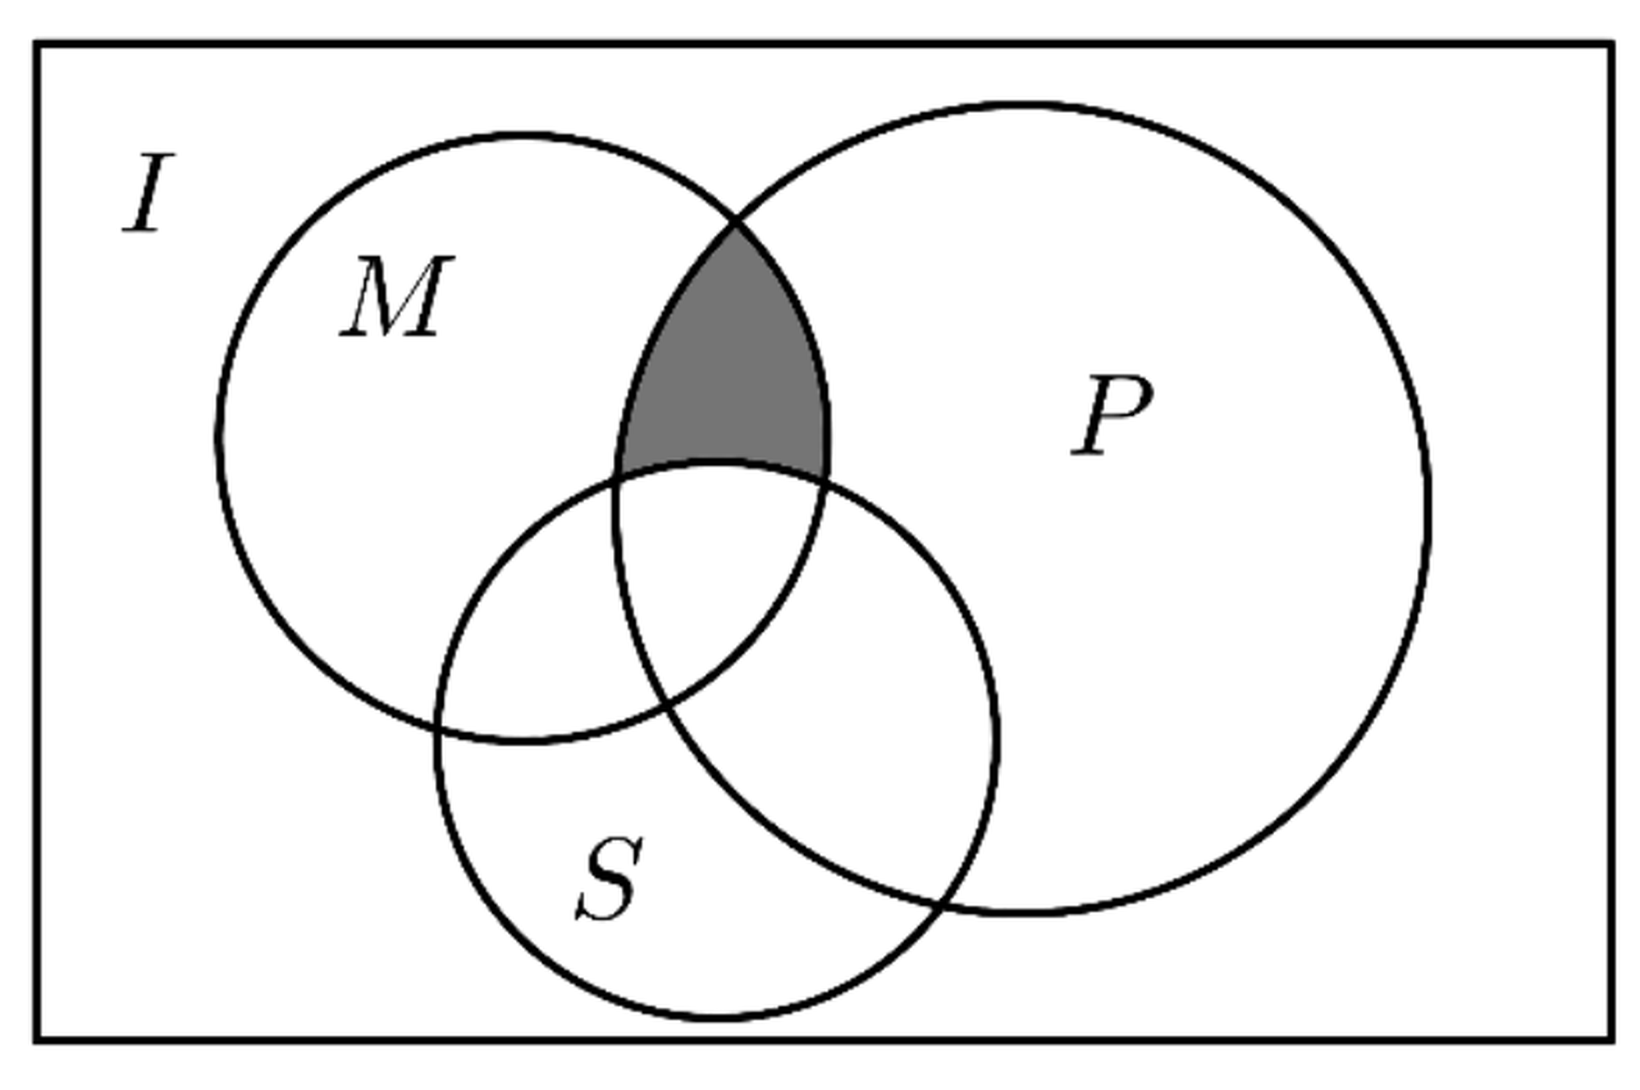
\includegraphics[width=0.42\textwidth]{figures/gao120_q15.png}
\end{center}

\keepwithprev
A. $(M\cap P)\cap S$\qquad\quad B. $(M\cap P)\cap\complement_{I}S$\qquad\quad C. $(M\cup P)\cap S$\qquad\quad D. $\complement_{I}(M\cap P)\cap S$

\ifanswer
\solbegin
\step{由已知中的 $Venn$ 图得阴影部分的元素属于 $M$，属于 $P$，但不属于 $S$，}
\step{所以阴影部分表示的集合为 $(M\cap P)\cap\complement_{I}S$，故选 $B$.}
\solend
\fi

\item 设集合 $P_1=\{x\mid x^2+ax+1>0\}$，$P_2=\{x\mid x^2+ax+2>0\}$，$Q_1=\{x\mid x^2+x+b>0\}$，$Q_2=\{x\mid x^2+2x+b>0\}$，其中 $a$、$b\in\R$，对于下列两个命题：①存在 $a$，$P_1$ 不是 $P_2$ 的子集；②存在 $b$ 使得 $Q_1$ 是 $Q_2$ 的子集. 下列说法正确的是\mbox{（\quad）}

\keepwithprev
A. ①是真命题，②是假命题\qquad\qquad B. ①是假命题，②是真命题

C. ①②都是真命题\qquad\qquad\qquad D. ①②都是假命题

\ifanswer
\solbegin
\step{对于集合 $P_1=\{x\mid x^2+ax+1>0\}$，$P_2=\{x\mid x^2+ax+2>0\}$，}
\step{得当 $m\in P_1$ 时，即 $m^2+am+1>0$，得 $m^2+am+2>0$，}
\step{即有 $m\in P_2$，得对任意 $a$，$P_1$ 是 $P_2$ 的子集，故①错误；}
\step{对于集合 $Q_1=\{x\mid x^2+x+b>0\}$，$Q_2=\{x\mid x^2+2x+b>0\}$，}
\step{当 $b=6$ 时，$Q_1=\{x\mid x^2+x+6>0\}=\R$，$Q_2=\{x\mid x^2+2x+6>0\}=\R$，}
\step{得 $Q_1$ 是 $Q_2$ 的子集，所以存在 $b$，使得 $Q_1$ 是 $Q_2$ 的子集，故②正确；}
\step{故选 $B$.}
\solend
\fi

\end{enumerate}

\bigsec{三、解答题}

\begin{enumerate}
\setcounter{enumi}{16}

\item (1) 已知 $x$、$y$ 都是实数，比较 $x^2+y^2$ 与 $4x-2y-5$ 的大小.

(2) 求解不等式组 $\begin{cases}x^2-4x+3\geqslant0\\\dfrac{x+3}{2x-1}\geqslant2\end{cases}$.

\ifanswer
\solbegin
\step{(1) $(x^2+y^2)-(4x-2y-5)=x^2-4x+y^2+2y+5=(x-2)^2+(y+1)^2\geqslant0$，}
\step{当 $x=2$，$y=-1$ 时，$x^2+y^2=4x-2y-5$.}
\step{当 $x\neq2$ 或 $y\neq-1$ 时，$x^2+y^2>4x-2y-5$.}
\step{(2) 由 $x^2-4x+3\geqslant0$ 得 $(x-1)(x-3)\geqslant0$，所以 $x\leqslant1$ 或 $x\geqslant3$；}
\step{由 $\dfrac{x+3}{2x-1}\geqslant2$，得 $\dfrac{x+3}{2x-1}-2=\dfrac{-3x+5}{2x-1}\geqslant0$，即 $\dfrac{3x-5}{2x-1}\leqslant0$，}
\step{所以 $\begin{cases}(3x-5)(2x-1)\leqslant0\\2x-1\neq0\end{cases}$，解得 $\dfrac12<x\leqslant\dfrac53$，}
\step{所以不等式组的解集是 $\left\{x\,\middle\vert\,\dfrac12<x\leqslant1\right\}$.}
\solend
\fi

\item 已知 $x_1$,$x_2$ 是一元二次方程 $4kx^2-4kx+k+1=0$ 的两个实数根.

(1) 是否存在实数 $k$，$(2x_1-x_2)(x_1-2x_2)=-\dfrac32$ 成立？若存在，求出 $k$ 的值；若不存在，请说明理由.

(2) 求使 $\dfrac{x_1}{x_2}+\dfrac{x_2}{x_1}-2$ 的值为整数的实数 $k$ 的整数值.

\ifanswer
\solbegin
\step{(1) 因为 $x_1$,$x_2$ 是一元二次方程 $4kx^2-4kx+k+1=0$ 的两个实数根，}
\step{所以 $\begin{cases}k\neq0\\16k^2-16k(k+1)\geqslant0\end{cases}$，所以 $k<0$，}
\step{由根与系数的关系得 $x_1+x_2=1$，$x_1x_2=\dfrac{k+1}{4k}$，}
\step{所以 $(2x_1-x_2)(x_1-2x_2)=2(x_1+x_2)^2-9x_1x_2=2-9\times\dfrac{k+1}{4k}=-\dfrac32$，}
\step{解得 $k=\dfrac95$，而 $k<0$，故不存在实数 $k$ 使得 $(2x_1-x_2)(x_1-2x_2)=-\dfrac32$ 成立.}
\step{(2) 由根与系数的关系得 $\dfrac{x_1}{x_2}+\dfrac{x_2}{x_1}-2=\dfrac{(x_1+x_2)^2}{x_1x_2}-4=-\dfrac4{k+1}$，}
\step{因为 $-\dfrac4{k+1}$ 的值为整数，而 $k$ 为整数，所以 $k+1$ 只能取 $\pm1$、$\pm2$、$\pm4$，}
\step{又 $k<0$，所以整数 $k$ 的值为 $-2$ 或 $-3$ 或 $-5$.}
\solend
\fi

\item 2026 年，某市低空经济蓬勃发展，一家物流企业开通“无人机即时配送”服务，并设立配送站. 经市场调研，该站每日配送单量 $y$（单位：单）与每单配送费 $x$（单位：元）满足关系式 $y=4800-200x$（其中 $4<x<24$）. 已知配送站每日的固定成本为 $19200$ 元，每完成一单配送，需支付电费、耗材费、设备保养费等可变成本，每单可变成本为 $4$ 元.

(1) 若要保证配送站每日利润 $W$（单位：元）不为负数，求每单配送费 $x$ 的取值范围；（每日利润 $=$ 每日配送总收入 $-$ 每日可变总成本 $-$ 每日固定成本）

(2) 为提升运力，该站购进一批新型无人机，购机费用为 $32$ 万元. 投入使用后，这批无人机使用 $t(t>0)$ 年的累计维保总费用为 $(2t^2+8t)$ 万元. 请问：这批无人机使用多少年后更新，可以使年平均总费用最低？请求出最低年平均总费用.（年平均总费用 $=$（购机费用 $+$ 维保总费用）$\div$ 使用年数）

\ifanswer
\solbegin
\step{(1) $W=xy-4y-19200=x(4800-200x)-4(4800-200x)-19200$}
\step{$=-200x^2+5600x-38400(4<x<24)$，}
\step{令 $W=-200x^2+5600x-38400\geqslant0$，即 $x^2-28x+192\leqslant0$，}
\step{解得 $12\leqslant x\leqslant16$，因此，要保证配送站每日利润 $W$ 不为负数，}
\step{每单配送费 $x$ 的取值范围为 $[12,16]$；}
\step{(2) 由题意，年平均总费用为 $N=\dfrac{2t^2+8t+32}{t}=2t+\dfrac{32}{t}+8$}
\step{$\geqslant2\sqrt{2t\cdot\dfrac{32}{t}}+8=16+8=24$，当且仅当 $2t=\dfrac{32}{t}$，即 $t=4$ 时取等号，}
\step{则这批无人机使用 $4$ 年后更新，可以使年平均总费用最低，}
\step{最低年平均总费用为 $24$ 万元.}
\solend
\fi

\item 已知 $A,B$，定义集合 $M_{(A,B)}=\{x\mid A<B\}$.

(1) 设 $A=\lvert x-4\rvert$,$B=2x$，求 $M_{(A,B)}$；

(2) 设 $A=ax^2+2ax-4$,$B=2x(x+2)$，当 $M_{(A,B)}=\R$ 时，求 $a$ 的取值范围；

(3) 设 $A=\lvert 2x-b\rvert$,$B=\dfrac{x+4b}{x-1}$,$C=2$，若 $M_{(A,C)}\cap M_{(B,C)}\neq\varnothing$，求 $b$ 的取值范围.

\ifanswer
\solbegin
\step{(1) 由定义，$x\in M_{(A,B)}$ 等价于 $\lvert x-4\rvert<2x$，}
\step{原不等式等价于 $-2x<x-4<2x$，即同时满足 $3x>4$ 与 $x>-4$，}
\step{解得 $x>\dfrac43$，所以 $M_{(A,B)}=\left(\dfrac43,+\infty\right)$.}
\step{(2) 由 $M_{(A,B)}=\R$，得 $ax^2+2ax-4<2x(x+2)$ 对任意 $x\in\R$ 恒成立，}
\step{得 $(a-2)(x+1)^2-a-2<0$.}
\step{当 $a>2$ 时，随着 $(x+1)^2$ 增大，左边可取正值，不符合题意；}
\step{当 $a=2$ 时，左边恒等于 $-4$，符合题意；}
\step{当 $a<2$ 时，左边在 $x=-1$ 处取得最大值 $-a-2$，}
\step{故恒成立的充要条件为 $-a-2<0$，即 $a>-2$；}
\step{综上，$a\in(-2,2]$.}
\step{(3) 由 $\lvert 2x-b\rvert<2$，得 $M_{(A,C)}=\left(\dfrac b2-1,\dfrac b2+1\right)$，记为 $I$.}
\step{由 $\dfrac{x+4b}{x-1}<2$，得 $\dfrac{x-(4b+2)}{x-1}>0$，其中 $x\neq1$.}
\step{①当 $b<-\dfrac14$ 时，$4b+2<1$，故 $M_{(B,C)}=(-\infty,4b+2)\cup(1,+\infty)$.}
\step{此时 $\dfrac b2+1<1$，所以 $I$ 与 $(1,+\infty)$ 没有公共元素.}
\step{两集合交集非空等价于 $\dfrac b2-1<4b+2$，解得 $b>-\dfrac67$.}
\step{因而本种情况得到 $-\dfrac67<b<-\dfrac14$.}
\step{②当 $b=-\dfrac14$ 时，$\dfrac{x+4b}{x-1}=1$，其中 $x\neq1$，故 $M_{(B,C)}=\{x\mid x\neq1\}$.}
\step{此时 $I=\left(-\dfrac98,\dfrac78\right)$，两集合交集非空.}
\step{③当 $b>-\dfrac14$ 时，$4b+2>1$，故 $M_{(B,C)}=(-\infty,1)\cup(4b+2,+\infty)$.}
\step{此时 $4b+2-\left(\dfrac b2+1\right)=\dfrac{7b}{2}+1>\dfrac18>0$，}
\step{所以 $I$ 与 $(4b+2,+\infty)$ 没有公共元素.}
\step{两集合交集非空等价于 $\dfrac b2-1<1$，解得 $b<4$.}
\step{因而本种情况得到 $-\dfrac14<b<4$.}
\step{综上，$b\in\left(-\dfrac67,4\right)$.}
\solend
\fi

\item 破晓同学阅读课外书籍时，发现笛卡尔积是代数和图论中一个很重要的课题. 对于非空数集 $A,B$，定义 $A\otimes B=\{(x,y)\mid x\in A$ 且 $y\in B\}$，将 $A\otimes B$ 称为“$A$ 与 $B$ 的笛卡尔积”.

(1) 若 $A=\{-1,0,1\}$,$B=\{-1,1\}$，求 $A\otimes B$ 和 $B\otimes A$；

(2) 试证明：“$A_1\otimes A_2=A_2\otimes A_1$”是“$A_1=A_2$”的充要条件；

(3) 若集合 $H$ 是有限集，将集合 $H$ 的元素个数记为 $\lvert H\rvert$. 已知 $\lvert A_1\otimes A_2\rvert=m^3(m\in\N^*)$，且存在实数 $a$ 满足 $\sqrt{\dfrac{\lvert A_1\otimes A_1\rvert+\lvert A_2\otimes A_2\rvert}{\lvert A_2\otimes A_1\rvert}}\geqslant a$ 对任意 $m\in\N^*$ 恒成立. 求 $a$ 的取值范围，并指明当 $a$ 取到最值时 $\lvert A_1\rvert$ 和 $\lvert A_2\rvert$ 满足的关系式及 $m$ 应满足的条件.

\ifanswer
\solbegin
\step{(1) 由题意得 $A\otimes B=\{(-1,-1),(-1,1),(0,-1),(0,1),(1,-1),(1,1)\}$，}
\step{$B\otimes A=\{(-1,-1),(-1,0),(-1,1),(1,-1),(1,0),(1,1)\}$；}
\step{(2) 若 $A_1=A_2$，设 $A_1=A_2=A$，}
\step{由定义得 $A_1\otimes A_2=\{(a,b)\mid a\in A$ 且 $b\in A\}=A_2\otimes A_1$，}
\step{所以“$A_1\otimes A_2=A_2\otimes A_1$”是“$A_1=A_2$”的必要条件；}
\step{若 $A_1\otimes A_2=A_2\otimes A_1$，对任意 $(a,b)\in A_1\otimes A_2$，均有 $(a,b)\in A_2\otimes A_1$，}
\step{即对任意 $a\in A_1,b\in A_2$，均有 $a\in A_2,b\in A_1$，}
\step{由任意性得 $A_1\subseteq A_2,A_2\subseteq A_1$，则 $A_1=A_2$，}
\step{所以“$A_1\otimes A_2=A_2\otimes A_1$”是“$A_1=A_2$”的充分条件；}
\step{综上所述，“$A_1\otimes A_2=A_2\otimes A_1$”是“$A_1=A_2$”的充要条件.}
\step{(3) 设 $\lvert A_1\rvert=c$,$\lvert A_2\rvert=d$,$c,d\in\N^*$，}
\step{则 $\lvert A_1\otimes A_2\rvert=\lvert A_2\otimes A_1\rvert=cd=m^3$,$\lvert A_1\otimes A_1\rvert=c^2$,$\lvert A_2\otimes A_2\rvert=d^2$，}
\step{得 $\sqrt{\dfrac{\lvert A_1\otimes A_1\rvert+\lvert A_2\otimes A_2\rvert}{\lvert A_2\otimes A_1\rvert}}=\sqrt{\dfrac{c^2+d^2}{cd}}=\sqrt{\dfrac cd+\dfrac dc}\geqslant\sqrt{2\sqrt{\dfrac cd\cdot\dfrac dc}}=\sqrt2$，}
\step{当且仅当 $\dfrac cd=\dfrac dc$，即 $c=d$ 时取等号，所以实数 $a$ 的取值范围是 $(-\infty,\sqrt2]$.}
\step{若 $a$ 取到最大值，则 $c=d$，即 $\lvert A_1\rvert=\lvert A_2\rvert$，得 $c^2=m^3$，}
\step{即 $c=\sqrt{m^3}=(\sqrt m)^3\in\N^*$，所以 $m=k^2,k\in\N^*$.}
\solend
\fi

\end{enumerate}

\end{document}
"
%
% 原始材料：微信公众号“魔都数学加油站”文章，作者破晓，2026-11-08 21:35 发布；
% 连载“27学年高一120”，原文标题“27学年高一120——2026-2027年上海市松江二中高一上10月月考”；
% 原文链接：https://mp.weixin.qq.com/s/hgDkaZX9M_IKhmr7CjQc1A。
% 正文为 10 张 PNG 页（第 8、10 页 2560×3620，其余 4762×6735），
% 题目下印有【解析】或【答案】，为讲评版。
% 题目、解析均据原图转录；卷面红色水印及公众号页脚未录入。
% 全卷 1 张插图：第 15 题的三集合 Venn 图（原卷印在题干右侧，本稿移至题干之后，
% 取原卷截图 2× LANCZOS 放大，见 figures/gao120_q15.png）。
%
% 卷首标题：原卷印作“2026-2027 年松江二中高一上 10 月月考”（公众号标题中的“上海市”
% 卷面标题行没有，本稿照卷面），年份区间按全稿惯例排 en dash；原卷未印副标题，本稿按题目内容
% 标为“集合与常用逻辑用语、不等式”（与 110／111／113／116／118 同）。
%
% 与原卷的排版差异：
%   ① 原文从第 3 题起，填空题编号为 3—12、选择题为 13—16、解答题为 17—21，本稿保留原题号；
%   ② 原卷每题下直接印【解析】／【答案】，本稿按全稿惯例置于答案版；第 3 题只印【答案】、
%      第 13、14 题把答案印在题干括号内且无【解析】，均另提 \ans{}；其余选择题答案在
%      解析末句“故选 …”，括号内留空；
%   ③ 原卷未印副标题，本稿按“知识模块”口径补出；
%   ④ 原卷填空横线按全稿惯例排为 \blankline[4.4em]；选择题括号排 \mbox{（\quad）}、
%      选项段前按惯例加 \keepwithprev；解答题不留作答区（原卷为讲评版，与 109—119 同）；
%   ⑤ 原卷数集排斜体 $R$、$N^*$，按全稿惯例改 \R、\N^*；绝对值排 \lvert…\rvert，
%      集合描述竖线排 \mid；补集记号照原卷排 \complement_I。
%
% 判别式字形：第 9 题解析作 $\triangle$（等边、扁），照录 \triangle。
%
% 子集符号：第 4 题题干与解析的 $A\subseteq B$、第 21 题 (2) 的 $A_1\subseteq A_2$ 印有下划线，
%   照录 \subseteq。
%
% 原卷存疑照录：第 12 题题干 $S=\{82,83,84,85,86,87,89\}$ 跳过 $88$ 只列 7 个数，
%   与其“8 种不同的值”自洽（不含 $88$），照录；第 19 题 (1) 的 $W$ 表达式
%   $x(4800-200x)-4(4800-200x)-19200$ 与最后结果 $[12,16]$ 一致。
%
% 行数核对：逐题数 \step 条数，合计 115 条（Q3：0；Q4：4；Q5：2；Q6：5；Q7：4；
% Q8：2；Q9：5；Q10：3；Q11：6；Q12：11；Q13：0；Q14：0；Q15：2；Q16：7；
% Q17：7；Q18：8；Q19：9；Q20：24；Q21：16），与原卷印刷行逐题相等
% （cases 块作一个印刷行计）。第 3 题只印【答案】、第 13、14 题括号内印答案且无解析，
% 均提 \ans{}，不计入 \step 账。
%
\documentclass[a4paper,11pt]{article}
\usepackage{common}

\begin{document}

\examtitlest[3]{2026--2027 年松江二中高一上 10 月月考}{集合与常用逻辑用语、不等式}

\bigsec{一、填空题}

\begin{enumerate}
\setcounter{enumi}{2}

\item 集合 $A=\{(x,y)\mid x+y=8\}$,$B=\{(x,y)\mid xy=12\}$，求 $A\cap B=$\blankline[4.4em].

\ifanswer
\ans{$\{(2,6),(6,2)\}$}
\fi

\item 设集合 $A=\{0,-a\}$,$B=\{1,a-2,2a-2\}$，若 $A\subseteq B$，则 $a=$\blankline[4.4em].

\ifanswer
\solbegin
\step{因为 $A\subseteq B$，}
\step{若 $a-2=0$，解得 $a=2$，此时 $A=\{0,-2\}$,$B=\{1,0,2\}$，不符合题意；}
\step{若 $2a-2=0$，解得 $a=1$，此时 $A=\{0,-1\}$,$B=\{1,-1,0\}$，符合题意；}
\step{综上所述，$a=1$.}
\solend
\fi

\item 设 $\alpha:0<x<a(a>0)$,$\beta:x<8-3a$，若 $\alpha$ 是 $\beta$ 的充分条件，则实数 $a$ 的取值范围是\blankline[4.4em].

\ifanswer
\solbegin
\step{由 $\alpha$ 是 $\beta$ 的充分条件得，$x\in(0,a)\Rightarrow x\in(-\infty,8-3a)$，}
\step{所以 $0<a\leqslant8-3a$，解得 $0<a\leqslant2$.}
\solend
\fi

\item 关于 $x$ 的不等式 $ax-b>0$ 的解集为 $(-\infty,1)$，则不等式 $\dfrac{x-2}{ax+b}<0$ 的解集为\blankline[4.4em].

\ifanswer
\solbegin
\step{因为关于 $x$ 的不等式 $ax-b>0$ 的解集为 $(-\infty,1)$，}
\step{所以 $a<0$ 且 $\dfrac ba=1$，则 $b=a$，}
\step{所以不等式 $\dfrac{x-2}{ax+b}<0$，即 $\dfrac{x-2}{ax+a}<0$，即 $\dfrac{x-2}{x+1}>0$，}
\step{等价于 $(x+1)(x-2)>0$，解得 $x>2$ 或 $x<-1$，}
\step{即解集为 $(-\infty,-1)\cup(2,+\infty)$.}
\solend
\fi

\item 若正实数 $x$、$y$ 满足 $2x+y+8xy=2$，则 $xy$ 的最大值为\blankline[4.4em].

\ifanswer
\solbegin
\step{因为正实数 $x$、$y$ 满足 $2x+y+8xy=2$，}
\step{所以 $2-8xy=2x+y\geqslant2\sqrt{2xy}$，}
\step{当且仅当 $y=2x$，即 $x=\dfrac14$，$y=\dfrac12$ 时取等号，解得 $0<xy\leqslant\dfrac18$，}
\step{故 $xy$ 的最大值为 $\dfrac18$.}
\solend
\fi

\item 已知 $1<a<3$，$-5<b<-2$，则 $\dfrac ab$ 的取值范围是\blankline[4.4em].

\ifanswer
\solbegin
\step{因为 $-5<b<-2$，所以 $2<-b<5$，$\dfrac15<-\dfrac1b<\dfrac12$，又 $1<a<3$，}
\step{得 $\dfrac15<-\dfrac ab<\dfrac32$，则 $-\dfrac32<\dfrac ab<-\dfrac15$，故 $\dfrac ab$ 的取值范围是 $\left(-\dfrac32,-\dfrac15\right)$.}
\solend
\fi

\item 若关于 $x$、$y$ 的方程组 $\begin{cases}y-kx-2=0\\y^2-4x-2y+1=0\end{cases}$ 的解集中只有一个元素，则实数 $k$ 的值为\blankline[4.4em].

\ifanswer
\solbegin
\step{由 $\begin{cases}y-kx-2=0\\y^2-4x-2y+1=0\end{cases}$ 消去 $y$ 整理得 $k^2x^2+(2k-4)x+1=0$.}
\step{当 $k\neq0$ 时，则 $\triangle=(2k-4)^2-4k^2=0$，解得 $k=1$，}
\step{此时方程组的解为 $\begin{cases}x=1\\y=3\end{cases}$，符合题意；}
\step{当 $k=0$ 时，解得 $x=\dfrac14$，此时方程组的解为 $\begin{cases}x=\dfrac14\\y=2\end{cases}$，符合题意；}
\step{综上，$k=0$ 或 $k=1$.}
\solend
\fi

\item 若集合 $A=\{0,1\}$，$B=\{x\mid x^2-mx-m>0,x\in\R\}$，且 $A\cap B=\{1\}$，则实数 $m$ 的取值范围为\blankline[4.4em].

\ifanswer
\solbegin
\step{因为集合 $A=\{0,1\}$，$B=\{x\mid x^2-mx-m>0,x\in\R\}$，且 $A\cap B=\{1\}$，}
\step{则 $1\in B$ 且 $0\notin B$，所以 $\begin{cases}1-m-m>0\\-m\leqslant0\end{cases}$，解得 $0\leqslant m<\dfrac12$，}
\step{所以实数 $m$ 的取值范围是 $\left[0,\dfrac12\right)$.}
\solend
\fi

\item 从集合 $U=\{a,b,c,d\}$ 的子集中选出两个不同的子集，需同时满足以下两个条件：(1) $a$、$b$ 都至少属于其中一个集合；(2) 对选出的两个子集，其中一个集合为另一个的子集，那么共有\blankline[4.4em]种不同的选法.

\ifanswer
\solbegin
\step{不妨设元素少的为 $A$，元素多的为 $B$，则 $B$ 必包含有 $a$、$b$；$A$ 为 $B$ 的真子集，}
\step{若 $B=\{a,b\}$，$A$ 为 $B$ 的真子集，共 $2^2-1=3$ 种，}
\step{若 $B=\{a,b,c\}$，$A$ 为 $B$ 的真子集，共 $2^3-1=7$ 种，}
\step{若 $B=\{a,b,d\}$，$A$ 为 $B$ 的真子集，共 $2^3-1=7$ 种，}
\step{若 $B=\{a,b,c,d\}$，$A$ 为 $B$ 的真子集，共 $2^4-1=15$ 种，}
\step{共有 $3+7+7+15=32$ 种.}
\solend
\fi

\item 已知 $a_1$、$a_2$、$\cdots$、$a_8$ 是 $8$ 个正整数，记 $S=\{a_{i_1}+a_{i_2}+\cdots+a_{i_7}\mid 1\leqslant i_1<i_2<\cdots<i_7\leqslant8\}$，其中 $i_1$、$i_2$、$\cdots$、$i_7\in\N^*$，若 $S=\{82,83,84,85,86,87,89\}$，则这 $8$ 个正整数中的最大数与最小数的积为\blankline[4.4em].

\ifanswer
\solbegin
\step{由题意得从 $8$ 个数中任取 $7$ 个数的和共有 $C_8^7=8$ 种不同的值，}
\step{但是 $82$，$83$，$84$，$85$，$86$，$87$，$89$ 只有 $7$ 个数，}
\step{得必有两种 $7$ 个数的和相等，设这个和为 $t(82\leqslant t\leqslant89)$，}
\step{令 $T=\sum\limits_{i=1}^{8}a_i$，那么，任取 $7$ 个数的和就等于 $T-a_i$，$i=1,2,\cdots,8$，}
\step{这 $8$ 个取值和的集合为 $S$，$S=\{T-a_1,T-a_2,\cdots,T-a_8\}$，}
\step{则 $\sum\limits_{i=1}^{8}(T-a_i)=8T-T=7T=82+83+84+85+86+87+89+t=596+t$.}
\step{因为 $T$ 为整数，所以 $596+t$ 是 $7$ 的倍数，}
\step{由 $596=7\times85+1$ 得 $1+t$ 是 $7$ 的倍数，}
\step{再因为 $82\leqslant t\leqslant89$，所以 $t=83$，得 $T=97$.}
\step{因此 $a_1$、$a_2$、$\cdots$、$a_8$ 中最大数为 $97-82=15$，最小数为 $97-89=8$，}
\step{因此，它们的积为 $120$.}
\solend
\fi

\end{enumerate}

\bigsec{二、选择题}

\begin{enumerate}
\setcounter{enumi}{12}

\item 已知 $a>b>0$，$c\in\R$，则下列不等式不一定成立的是\mbox{（\quad）}% 原卷把答案“$B$”印在题干括号内、无【解析】

\keepwithprev
A. $a-c>b-c$\qquad\quad B. $ac>bc$\qquad\quad C. $\dfrac1a<\dfrac1b$\qquad\quad D. $\dfrac{a+b}{2}>\sqrt{ab}$

\ifanswer
\ans{$B$}
\fi

\item 命题“对任意的 $x\in\R,x^3-x^2+1\leqslant0$”的否定是\mbox{（\quad）}% 原卷把答案“$C$”印在题干括号内、无【解析】

\keepwithprev
A. 不存在 $x\in\R,x^3-x^2+1\leqslant0$\qquad B. 存在 $x\in\R,x^3-x^2+1\leqslant0$

C. 存在 $x\in\R,x^3-x^2+1>0$\qquad\quad D. 对任意的 $x\in\R,x^3-x^2+1>0$

\ifanswer
\ans{$C$}
\fi

% 第 15 题是“题干 + 图 + 选项”约 6.5cm 的一整块，\keepwithprev 只挡得住“图—选项”，
% 挡不住夹在中间的图——实测断点落在题干之后（切页审计 A 类）。故照 高一30／高一26 成例
% 在题前先量一次页高，不够就把整块一起挪到次页。
\needvspace{7cm}
\item 如图，$I$ 是全集，$M$、$P$、$S$ 是 $I$ 的三个子集，则阴影部分所表示的集合是\mbox{（\quad）}

\begin{center}
% 图取原卷截图（第 4 页题干右侧）、2× LANCZOS 放大，本稿移至题干之后
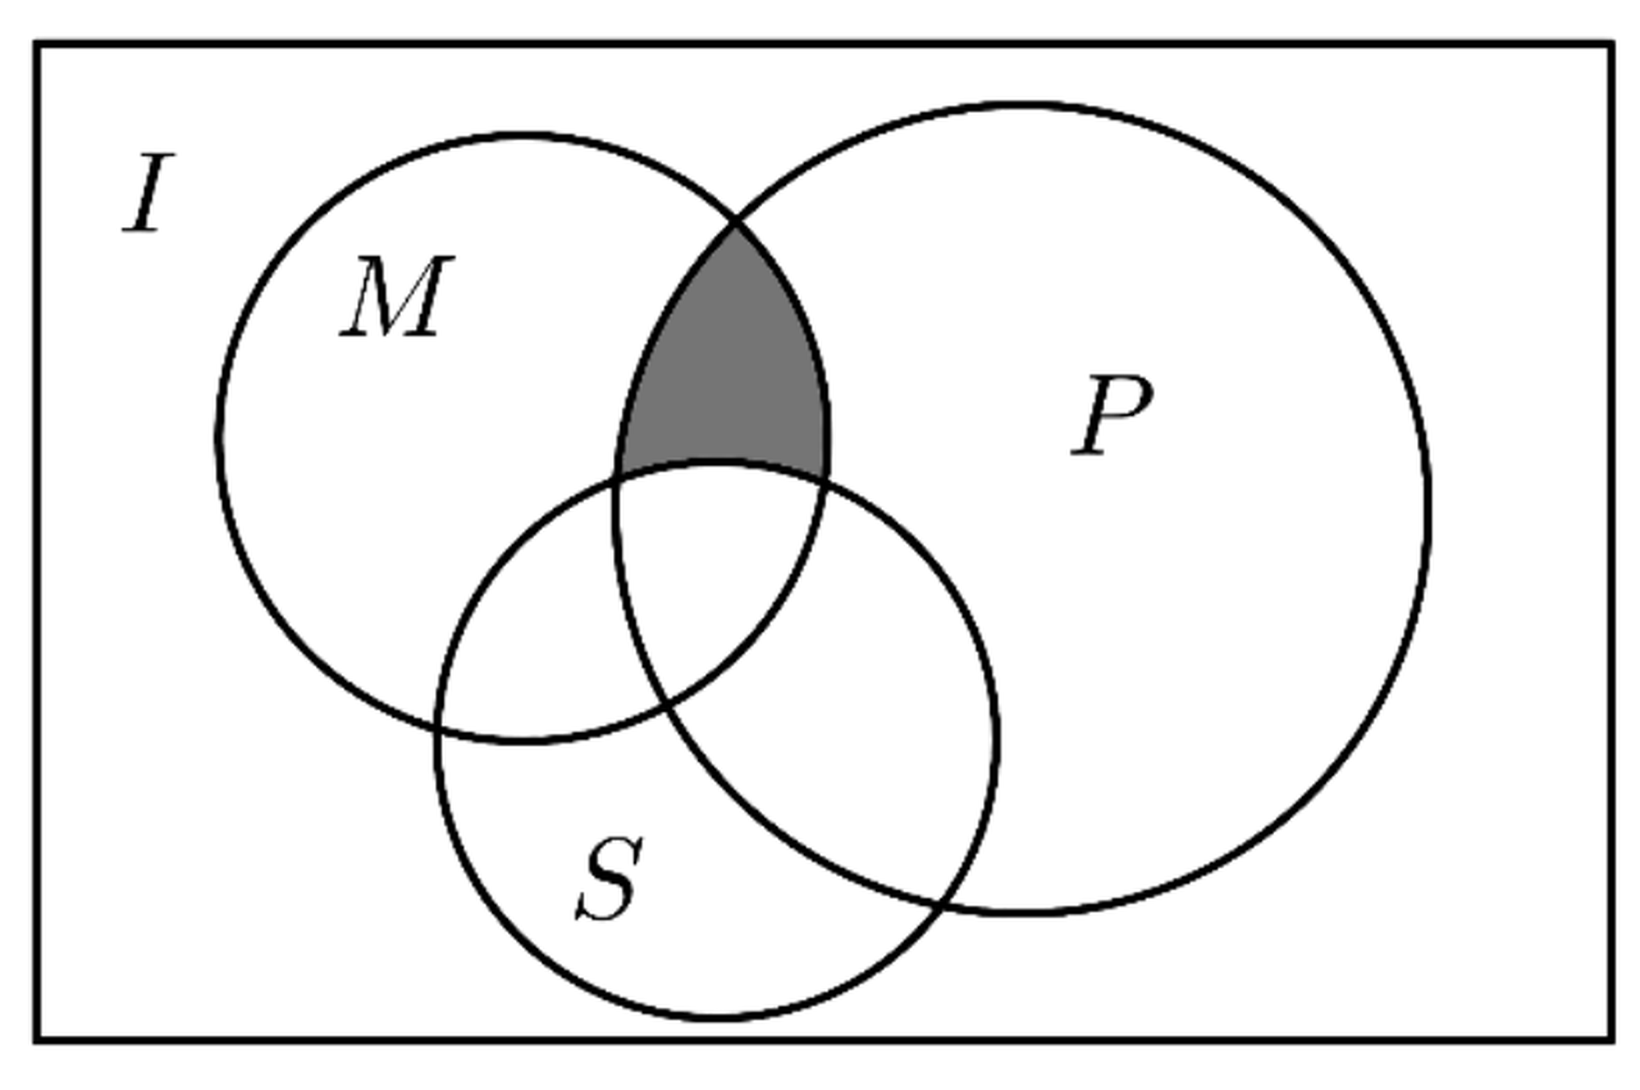
\includegraphics[width=0.42\textwidth]{figures/gao120_q15.png}
\end{center}

\keepwithprev
A. $(M\cap P)\cap S$\qquad\quad B. $(M\cap P)\cap\complement_{I}S$\qquad\quad C. $(M\cup P)\cap S$\qquad\quad D. $\complement_{I}(M\cap P)\cap S$

\ifanswer
\solbegin
\step{由已知中的 $Venn$ 图得阴影部分的元素属于 $M$，属于 $P$，但不属于 $S$，}
\step{所以阴影部分表示的集合为 $(M\cap P)\cap\complement_{I}S$，故选 $B$.}
\solend
\fi

\item 设集合 $P_1=\{x\mid x^2+ax+1>0\}$，$P_2=\{x\mid x^2+ax+2>0\}$，$Q_1=\{x\mid x^2+x+b>0\}$，$Q_2=\{x\mid x^2+2x+b>0\}$，其中 $a$、$b\in\R$，对于下列两个命题：①存在 $a$，$P_1$ 不是 $P_2$ 的子集；②存在 $b$ 使得 $Q_1$ 是 $Q_2$ 的子集. 下列说法正确的是\mbox{（\quad）}

\keepwithprev
A. ①是真命题，②是假命题\qquad\qquad B. ①是假命题，②是真命题

C. ①②都是真命题\qquad\qquad\qquad D. ①②都是假命题

\ifanswer
\solbegin
\step{对于集合 $P_1=\{x\mid x^2+ax+1>0\}$，$P_2=\{x\mid x^2+ax+2>0\}$，}
\step{得当 $m\in P_1$ 时，即 $m^2+am+1>0$，得 $m^2+am+2>0$，}
\step{即有 $m\in P_2$，得对任意 $a$，$P_1$ 是 $P_2$ 的子集，故①错误；}
\step{对于集合 $Q_1=\{x\mid x^2+x+b>0\}$，$Q_2=\{x\mid x^2+2x+b>0\}$，}
\step{当 $b=6$ 时，$Q_1=\{x\mid x^2+x+6>0\}=\R$，$Q_2=\{x\mid x^2+2x+6>0\}=\R$，}
\step{得 $Q_1$ 是 $Q_2$ 的子集，所以存在 $b$，使得 $Q_1$ 是 $Q_2$ 的子集，故②正确；}
\step{故选 $B$.}
\solend
\fi

\end{enumerate}

\bigsec{三、解答题}

\begin{enumerate}
\setcounter{enumi}{16}

\item (1) 已知 $x$、$y$ 都是实数，比较 $x^2+y^2$ 与 $4x-2y-5$ 的大小.

(2) 求解不等式组 $\begin{cases}x^2-4x+3\geqslant0\\\dfrac{x+3}{2x-1}\geqslant2\end{cases}$.

\ifanswer
\solbegin
\step{(1) $(x^2+y^2)-(4x-2y-5)=x^2-4x+y^2+2y+5=(x-2)^2+(y+1)^2\geqslant0$，}
\step{当 $x=2$，$y=-1$ 时，$x^2+y^2=4x-2y-5$.}
\step{当 $x\neq2$ 或 $y\neq-1$ 时，$x^2+y^2>4x-2y-5$.}
\step{(2) 由 $x^2-4x+3\geqslant0$ 得 $(x-1)(x-3)\geqslant0$，所以 $x\leqslant1$ 或 $x\geqslant3$；}
\step{由 $\dfrac{x+3}{2x-1}\geqslant2$，得 $\dfrac{x+3}{2x-1}-2=\dfrac{-3x+5}{2x-1}\geqslant0$，即 $\dfrac{3x-5}{2x-1}\leqslant0$，}
\step{所以 $\begin{cases}(3x-5)(2x-1)\leqslant0\\2x-1\neq0\end{cases}$，解得 $\dfrac12<x\leqslant\dfrac53$，}
\step{所以不等式组的解集是 $\left\{x\,\middle\vert\,\dfrac12<x\leqslant1\right\}$.}
\solend
\fi

\item 已知 $x_1$,$x_2$ 是一元二次方程 $4kx^2-4kx+k+1=0$ 的两个实数根.

(1) 是否存在实数 $k$，$(2x_1-x_2)(x_1-2x_2)=-\dfrac32$ 成立？若存在，求出 $k$ 的值；若不存在，请说明理由.

(2) 求使 $\dfrac{x_1}{x_2}+\dfrac{x_2}{x_1}-2$ 的值为整数的实数 $k$ 的整数值.

\ifanswer
\solbegin
\step{(1) 因为 $x_1$,$x_2$ 是一元二次方程 $4kx^2-4kx+k+1=0$ 的两个实数根，}
\step{所以 $\begin{cases}k\neq0\\16k^2-16k(k+1)\geqslant0\end{cases}$，所以 $k<0$，}
\step{由根与系数的关系得 $x_1+x_2=1$，$x_1x_2=\dfrac{k+1}{4k}$，}
\step{所以 $(2x_1-x_2)(x_1-2x_2)=2(x_1+x_2)^2-9x_1x_2=2-9\times\dfrac{k+1}{4k}=-\dfrac32$，}
\step{解得 $k=\dfrac95$，而 $k<0$，故不存在实数 $k$ 使得 $(2x_1-x_2)(x_1-2x_2)=-\dfrac32$ 成立.}
\step{(2) 由根与系数的关系得 $\dfrac{x_1}{x_2}+\dfrac{x_2}{x_1}-2=\dfrac{(x_1+x_2)^2}{x_1x_2}-4=-\dfrac4{k+1}$，}
\step{因为 $-\dfrac4{k+1}$ 的值为整数，而 $k$ 为整数，所以 $k+1$ 只能取 $\pm1$、$\pm2$、$\pm4$，}
\step{又 $k<0$，所以整数 $k$ 的值为 $-2$ 或 $-3$ 或 $-5$.}
\solend
\fi

\item 2026 年，某市低空经济蓬勃发展，一家物流企业开通“无人机即时配送”服务，并设立配送站. 经市场调研，该站每日配送单量 $y$（单位：单）与每单配送费 $x$（单位：元）满足关系式 $y=4800-200x$（其中 $4<x<24$）. 已知配送站每日的固定成本为 $19200$ 元，每完成一单配送，需支付电费、耗材费、设备保养费等可变成本，每单可变成本为 $4$ 元.

(1) 若要保证配送站每日利润 $W$（单位：元）不为负数，求每单配送费 $x$ 的取值范围；（每日利润 $=$ 每日配送总收入 $-$ 每日可变总成本 $-$ 每日固定成本）

(2) 为提升运力，该站购进一批新型无人机，购机费用为 $32$ 万元. 投入使用后，这批无人机使用 $t(t>0)$ 年的累计维保总费用为 $(2t^2+8t)$ 万元. 请问：这批无人机使用多少年后更新，可以使年平均总费用最低？请求出最低年平均总费用.（年平均总费用 $=$（购机费用 $+$ 维保总费用）$\div$ 使用年数）

\ifanswer
\solbegin
\step{(1) $W=xy-4y-19200=x(4800-200x)-4(4800-200x)-19200$}
\step{$=-200x^2+5600x-38400(4<x<24)$，}
\step{令 $W=-200x^2+5600x-38400\geqslant0$，即 $x^2-28x+192\leqslant0$，}
\step{解得 $12\leqslant x\leqslant16$，因此，要保证配送站每日利润 $W$ 不为负数，}
\step{每单配送费 $x$ 的取值范围为 $[12,16]$；}
\step{(2) 由题意，年平均总费用为 $N=\dfrac{2t^2+8t+32}{t}=2t+\dfrac{32}{t}+8$}
\step{$\geqslant2\sqrt{2t\cdot\dfrac{32}{t}}+8=16+8=24$，当且仅当 $2t=\dfrac{32}{t}$，即 $t=4$ 时取等号，}
\step{则这批无人机使用 $4$ 年后更新，可以使年平均总费用最低，}
\step{最低年平均总费用为 $24$ 万元.}
\solend
\fi

\item 已知 $A,B$，定义集合 $M_{(A,B)}=\{x\mid A<B\}$.

(1) 设 $A=\lvert x-4\rvert$,$B=2x$，求 $M_{(A,B)}$；

(2) 设 $A=ax^2+2ax-4$,$B=2x(x+2)$，当 $M_{(A,B)}=\R$ 时，求 $a$ 的取值范围；

(3) 设 $A=\lvert 2x-b\rvert$,$B=\dfrac{x+4b}{x-1}$,$C=2$，若 $M_{(A,C)}\cap M_{(B,C)}\neq\varnothing$，求 $b$ 的取值范围.

\ifanswer
\solbegin
\step{(1) 由定义，$x\in M_{(A,B)}$ 等价于 $\lvert x-4\rvert<2x$，}
\step{原不等式等价于 $-2x<x-4<2x$，即同时满足 $3x>4$ 与 $x>-4$，}
\step{解得 $x>\dfrac43$，所以 $M_{(A,B)}=\left(\dfrac43,+\infty\right)$.}
\step{(2) 由 $M_{(A,B)}=\R$，得 $ax^2+2ax-4<2x(x+2)$ 对任意 $x\in\R$ 恒成立，}
\step{得 $(a-2)(x+1)^2-a-2<0$.}
\step{当 $a>2$ 时，随着 $(x+1)^2$ 增大，左边可取正值，不符合题意；}
\step{当 $a=2$ 时，左边恒等于 $-4$，符合题意；}
\step{当 $a<2$ 时，左边在 $x=-1$ 处取得最大值 $-a-2$，}
\step{故恒成立的充要条件为 $-a-2<0$，即 $a>-2$；}
\step{综上，$a\in(-2,2]$.}
\step{(3) 由 $\lvert 2x-b\rvert<2$，得 $M_{(A,C)}=\left(\dfrac b2-1,\dfrac b2+1\right)$，记为 $I$.}
\step{由 $\dfrac{x+4b}{x-1}<2$，得 $\dfrac{x-(4b+2)}{x-1}>0$，其中 $x\neq1$.}
\step{①当 $b<-\dfrac14$ 时，$4b+2<1$，故 $M_{(B,C)}=(-\infty,4b+2)\cup(1,+\infty)$.}
\step{此时 $\dfrac b2+1<1$，所以 $I$ 与 $(1,+\infty)$ 没有公共元素.}
\step{两集合交集非空等价于 $\dfrac b2-1<4b+2$，解得 $b>-\dfrac67$.}
\step{因而本种情况得到 $-\dfrac67<b<-\dfrac14$.}
\step{②当 $b=-\dfrac14$ 时，$\dfrac{x+4b}{x-1}=1$，其中 $x\neq1$，故 $M_{(B,C)}=\{x\mid x\neq1\}$.}
\step{此时 $I=\left(-\dfrac98,\dfrac78\right)$，两集合交集非空.}
\step{③当 $b>-\dfrac14$ 时，$4b+2>1$，故 $M_{(B,C)}=(-\infty,1)\cup(4b+2,+\infty)$.}
\step{此时 $4b+2-\left(\dfrac b2+1\right)=\dfrac{7b}{2}+1>\dfrac18>0$，}
\step{所以 $I$ 与 $(4b+2,+\infty)$ 没有公共元素.}
\step{两集合交集非空等价于 $\dfrac b2-1<1$，解得 $b<4$.}
\step{因而本种情况得到 $-\dfrac14<b<4$.}
\step{综上，$b\in\left(-\dfrac67,4\right)$.}
\solend
\fi

\item 破晓同学阅读课外书籍时，发现笛卡尔积是代数和图论中一个很重要的课题. 对于非空数集 $A,B$，定义 $A\otimes B=\{(x,y)\mid x\in A$ 且 $y\in B\}$，将 $A\otimes B$ 称为“$A$ 与 $B$ 的笛卡尔积”.

(1) 若 $A=\{-1,0,1\}$,$B=\{-1,1\}$，求 $A\otimes B$ 和 $B\otimes A$；

(2) 试证明：“$A_1\otimes A_2=A_2\otimes A_1$”是“$A_1=A_2$”的充要条件；

(3) 若集合 $H$ 是有限集，将集合 $H$ 的元素个数记为 $\lvert H\rvert$. 已知 $\lvert A_1\otimes A_2\rvert=m^3(m\in\N^*)$，且存在实数 $a$ 满足 $\sqrt{\dfrac{\lvert A_1\otimes A_1\rvert+\lvert A_2\otimes A_2\rvert}{\lvert A_2\otimes A_1\rvert}}\geqslant a$ 对任意 $m\in\N^*$ 恒成立. 求 $a$ 的取值范围，并指明当 $a$ 取到最值时 $\lvert A_1\rvert$ 和 $\lvert A_2\rvert$ 满足的关系式及 $m$ 应满足的条件.

\ifanswer
\solbegin
\step{(1) 由题意得 $A\otimes B=\{(-1,-1),(-1,1),(0,-1),(0,1),(1,-1),(1,1)\}$，}
\step{$B\otimes A=\{(-1,-1),(-1,0),(-1,1),(1,-1),(1,0),(1,1)\}$；}
\step{(2) 若 $A_1=A_2$，设 $A_1=A_2=A$，}
\step{由定义得 $A_1\otimes A_2=\{(a,b)\mid a\in A$ 且 $b\in A\}=A_2\otimes A_1$，}
\step{所以“$A_1\otimes A_2=A_2\otimes A_1$”是“$A_1=A_2$”的必要条件；}
\step{若 $A_1\otimes A_2=A_2\otimes A_1$，对任意 $(a,b)\in A_1\otimes A_2$，均有 $(a,b)\in A_2\otimes A_1$，}
\step{即对任意 $a\in A_1,b\in A_2$，均有 $a\in A_2,b\in A_1$，}
\step{由任意性得 $A_1\subseteq A_2,A_2\subseteq A_1$，则 $A_1=A_2$，}
\step{所以“$A_1\otimes A_2=A_2\otimes A_1$”是“$A_1=A_2$”的充分条件；}
\step{综上所述，“$A_1\otimes A_2=A_2\otimes A_1$”是“$A_1=A_2$”的充要条件.}
\step{(3) 设 $\lvert A_1\rvert=c$,$\lvert A_2\rvert=d$,$c,d\in\N^*$，}
\step{则 $\lvert A_1\otimes A_2\rvert=\lvert A_2\otimes A_1\rvert=cd=m^3$,$\lvert A_1\otimes A_1\rvert=c^2$,$\lvert A_2\otimes A_2\rvert=d^2$，}
\step{得 $\sqrt{\dfrac{\lvert A_1\otimes A_1\rvert+\lvert A_2\otimes A_2\rvert}{\lvert A_2\otimes A_1\rvert}}=\sqrt{\dfrac{c^2+d^2}{cd}}=\sqrt{\dfrac cd+\dfrac dc}\geqslant\sqrt{2\sqrt{\dfrac cd\cdot\dfrac dc}}=\sqrt2$，}
\step{当且仅当 $\dfrac cd=\dfrac dc$，即 $c=d$ 时取等号，所以实数 $a$ 的取值范围是 $(-\infty,\sqrt2]$.}
\step{若 $a$ 取到最大值，则 $c=d$，即 $\lvert A_1\rvert=\lvert A_2\rvert$，得 $c^2=m^3$，}
\step{即 $c=\sqrt{m^3}=(\sqrt m)^3\in\N^*$，所以 $m=k^2,k\in\N^*$.}
\solend
\fi

\end{enumerate}

\end{document}
"
%
% 原始材料：微信公众号“魔都数学加油站”文章，作者破晓，2026-11-08 21:35 发布；
% 连载“27学年高一120”，原文标题“27学年高一120——2026-2027年上海市松江二中高一上10月月考”；
% 原文链接：https://mp.weixin.qq.com/s/hgDkaZX9M_IKhmr7CjQc1A。
% 正文为 10 张 PNG 页（第 8、10 页 2560×3620，其余 4762×6735），
% 题目下印有【解析】或【答案】，为讲评版。
% 题目、解析均据原图转录；卷面红色水印及公众号页脚未录入。
% 全卷 1 张插图：第 15 题的三集合 Venn 图（原卷印在题干右侧，本稿移至题干之后，
% 取原卷截图 2× LANCZOS 放大，见 figures/gao120_q15.png）。
%
% 卷首标题：原卷印作“2026-2027 年松江二中高一上 10 月月考”（公众号标题中的“上海市”
% 卷面标题行没有，本稿照卷面），年份区间按全稿惯例排 en dash；原卷未印副标题，本稿按题目内容
% 标为“集合与常用逻辑用语、不等式”（与 110／111／113／116／118 同）。
%
% 与原卷的排版差异：
%   ① 原文从第 3 题起，填空题编号为 3—12、选择题为 13—16、解答题为 17—21，本稿保留原题号；
%   ② 原卷每题下直接印【解析】／【答案】，本稿按全稿惯例置于答案版；第 3 题只印【答案】、
%      第 13、14 题把答案印在题干括号内且无【解析】，均另提 \ans{}；其余选择题答案在
%      解析末句“故选 …”，括号内留空；
%   ③ 原卷未印副标题，本稿按“知识模块”口径补出；
%   ④ 原卷填空横线按全稿惯例排为 \blankline[4.4em]；选择题括号排 \mbox{（\quad）}、
%      选项段前按惯例加 \keepwithprev；解答题不留作答区（原卷为讲评版，与 109—119 同）；
%   ⑤ 原卷数集排斜体 $R$、$N^*$，按全稿惯例改 \R、\N^*；绝对值排 \lvert…\rvert，
%      集合描述竖线排 \mid；补集记号照原卷排 \complement_I。
%
% 判别式字形：第 9 题解析作 $\triangle$（等边、扁），照录 \triangle。
%
% 子集符号：第 4 题题干与解析的 $A\subseteq B$、第 21 题 (2) 的 $A_1\subseteq A_2$ 印有下划线，
%   照录 \subseteq。
%
% 原卷存疑照录：第 12 题题干 $S=\{82,83,84,85,86,87,89\}$ 跳过 $88$ 只列 7 个数，
%   与其“8 种不同的值”自洽（不含 $88$），照录；第 19 题 (1) 的 $W$ 表达式
%   $x(4800-200x)-4(4800-200x)-19200$ 与最后结果 $[12,16]$ 一致。
%
% 行数核对：逐题数 \step 条数，合计 115 条（Q3：0；Q4：4；Q5：2；Q6：5；Q7：4；
% Q8：2；Q9：5；Q10：3；Q11：6；Q12：11；Q13：0；Q14：0；Q15：2；Q16：7；
% Q17：7；Q18：8；Q19：9；Q20：24；Q21：16），与原卷印刷行逐题相等
% （cases 块作一个印刷行计）。第 3 题只印【答案】、第 13、14 题括号内印答案且无解析，
% 均提 \ans{}，不计入 \step 账。
%
\documentclass[a4paper,11pt]{article}
\usepackage{common}

\begin{document}

\examtitlest[3]{2026--2027 年松江二中高一上 10 月月考}{集合与常用逻辑用语、不等式}

\bigsec{一、填空题}

\begin{enumerate}
\setcounter{enumi}{2}

\item 集合 $A=\{(x,y)\mid x+y=8\}$,$B=\{(x,y)\mid xy=12\}$，求 $A\cap B=$\blankline[4.4em].

\ifanswer
\ans{$\{(2,6),(6,2)\}$}
\fi

\item 设集合 $A=\{0,-a\}$,$B=\{1,a-2,2a-2\}$，若 $A\subseteq B$，则 $a=$\blankline[4.4em].

\ifanswer
\solbegin
\step{因为 $A\subseteq B$，}
\step{若 $a-2=0$，解得 $a=2$，此时 $A=\{0,-2\}$,$B=\{1,0,2\}$，不符合题意；}
\step{若 $2a-2=0$，解得 $a=1$，此时 $A=\{0,-1\}$,$B=\{1,-1,0\}$，符合题意；}
\step{综上所述，$a=1$.}
\solend
\fi

\item 设 $\alpha:0<x<a(a>0)$,$\beta:x<8-3a$，若 $\alpha$ 是 $\beta$ 的充分条件，则实数 $a$ 的取值范围是\blankline[4.4em].

\ifanswer
\solbegin
\step{由 $\alpha$ 是 $\beta$ 的充分条件得，$x\in(0,a)\Rightarrow x\in(-\infty,8-3a)$，}
\step{所以 $0<a\leqslant8-3a$，解得 $0<a\leqslant2$.}
\solend
\fi

\item 关于 $x$ 的不等式 $ax-b>0$ 的解集为 $(-\infty,1)$，则不等式 $\dfrac{x-2}{ax+b}<0$ 的解集为\blankline[4.4em].

\ifanswer
\solbegin
\step{因为关于 $x$ 的不等式 $ax-b>0$ 的解集为 $(-\infty,1)$，}
\step{所以 $a<0$ 且 $\dfrac ba=1$，则 $b=a$，}
\step{所以不等式 $\dfrac{x-2}{ax+b}<0$，即 $\dfrac{x-2}{ax+a}<0$，即 $\dfrac{x-2}{x+1}>0$，}
\step{等价于 $(x+1)(x-2)>0$，解得 $x>2$ 或 $x<-1$，}
\step{即解集为 $(-\infty,-1)\cup(2,+\infty)$.}
\solend
\fi

\item 若正实数 $x$、$y$ 满足 $2x+y+8xy=2$，则 $xy$ 的最大值为\blankline[4.4em].

\ifanswer
\solbegin
\step{因为正实数 $x$、$y$ 满足 $2x+y+8xy=2$，}
\step{所以 $2-8xy=2x+y\geqslant2\sqrt{2xy}$，}
\step{当且仅当 $y=2x$，即 $x=\dfrac14$，$y=\dfrac12$ 时取等号，解得 $0<xy\leqslant\dfrac18$，}
\step{故 $xy$ 的最大值为 $\dfrac18$.}
\solend
\fi

\item 已知 $1<a<3$，$-5<b<-2$，则 $\dfrac ab$ 的取值范围是\blankline[4.4em].

\ifanswer
\solbegin
\step{因为 $-5<b<-2$，所以 $2<-b<5$，$\dfrac15<-\dfrac1b<\dfrac12$，又 $1<a<3$，}
\step{得 $\dfrac15<-\dfrac ab<\dfrac32$，则 $-\dfrac32<\dfrac ab<-\dfrac15$，故 $\dfrac ab$ 的取值范围是 $\left(-\dfrac32,-\dfrac15\right)$.}
\solend
\fi

\item 若关于 $x$、$y$ 的方程组 $\begin{cases}y-kx-2=0\\y^2-4x-2y+1=0\end{cases}$ 的解集中只有一个元素，则实数 $k$ 的值为\blankline[4.4em].

\ifanswer
\solbegin
\step{由 $\begin{cases}y-kx-2=0\\y^2-4x-2y+1=0\end{cases}$ 消去 $y$ 整理得 $k^2x^2+(2k-4)x+1=0$.}
\step{当 $k\neq0$ 时，则 $\triangle=(2k-4)^2-4k^2=0$，解得 $k=1$，}
\step{此时方程组的解为 $\begin{cases}x=1\\y=3\end{cases}$，符合题意；}
\step{当 $k=0$ 时，解得 $x=\dfrac14$，此时方程组的解为 $\begin{cases}x=\dfrac14\\y=2\end{cases}$，符合题意；}
\step{综上，$k=0$ 或 $k=1$.}
\solend
\fi

\item 若集合 $A=\{0,1\}$，$B=\{x\mid x^2-mx-m>0,x\in\R\}$，且 $A\cap B=\{1\}$，则实数 $m$ 的取值范围为\blankline[4.4em].

\ifanswer
\solbegin
\step{因为集合 $A=\{0,1\}$，$B=\{x\mid x^2-mx-m>0,x\in\R\}$，且 $A\cap B=\{1\}$，}
\step{则 $1\in B$ 且 $0\notin B$，所以 $\begin{cases}1-m-m>0\\-m\leqslant0\end{cases}$，解得 $0\leqslant m<\dfrac12$，}
\step{所以实数 $m$ 的取值范围是 $\left[0,\dfrac12\right)$.}
\solend
\fi

\item 从集合 $U=\{a,b,c,d\}$ 的子集中选出两个不同的子集，需同时满足以下两个条件：(1) $a$、$b$ 都至少属于其中一个集合；(2) 对选出的两个子集，其中一个集合为另一个的子集，那么共有\blankline[4.4em]种不同的选法.

\ifanswer
\solbegin
\step{不妨设元素少的为 $A$，元素多的为 $B$，则 $B$ 必包含有 $a$、$b$；$A$ 为 $B$ 的真子集，}
\step{若 $B=\{a,b\}$，$A$ 为 $B$ 的真子集，共 $2^2-1=3$ 种，}
\step{若 $B=\{a,b,c\}$，$A$ 为 $B$ 的真子集，共 $2^3-1=7$ 种，}
\step{若 $B=\{a,b,d\}$，$A$ 为 $B$ 的真子集，共 $2^3-1=7$ 种，}
\step{若 $B=\{a,b,c,d\}$，$A$ 为 $B$ 的真子集，共 $2^4-1=15$ 种，}
\step{共有 $3+7+7+15=32$ 种.}
\solend
\fi

\item 已知 $a_1$、$a_2$、$\cdots$、$a_8$ 是 $8$ 个正整数，记 $S=\{a_{i_1}+a_{i_2}+\cdots+a_{i_7}\mid 1\leqslant i_1<i_2<\cdots<i_7\leqslant8\}$，其中 $i_1$、$i_2$、$\cdots$、$i_7\in\N^*$，若 $S=\{82,83,84,85,86,87,89\}$，则这 $8$ 个正整数中的最大数与最小数的积为\blankline[4.4em].

\ifanswer
\solbegin
\step{由题意得从 $8$ 个数中任取 $7$ 个数的和共有 $C_8^7=8$ 种不同的值，}
\step{但是 $82$，$83$，$84$，$85$，$86$，$87$，$89$ 只有 $7$ 个数，}
\step{得必有两种 $7$ 个数的和相等，设这个和为 $t(82\leqslant t\leqslant89)$，}
\step{令 $T=\sum\limits_{i=1}^{8}a_i$，那么，任取 $7$ 个数的和就等于 $T-a_i$，$i=1,2,\cdots,8$，}
\step{这 $8$ 个取值和的集合为 $S$，$S=\{T-a_1,T-a_2,\cdots,T-a_8\}$，}
\step{则 $\sum\limits_{i=1}^{8}(T-a_i)=8T-T=7T=82+83+84+85+86+87+89+t=596+t$.}
\step{因为 $T$ 为整数，所以 $596+t$ 是 $7$ 的倍数，}
\step{由 $596=7\times85+1$ 得 $1+t$ 是 $7$ 的倍数，}
\step{再因为 $82\leqslant t\leqslant89$，所以 $t=83$，得 $T=97$.}
\step{因此 $a_1$、$a_2$、$\cdots$、$a_8$ 中最大数为 $97-82=15$，最小数为 $97-89=8$，}
\step{因此，它们的积为 $120$.}
\solend
\fi

\end{enumerate}

\bigsec{二、选择题}

\begin{enumerate}
\setcounter{enumi}{12}

\item 已知 $a>b>0$，$c\in\R$，则下列不等式不一定成立的是\mbox{（\quad）}% 原卷把答案“$B$”印在题干括号内、无【解析】

\keepwithprev
A. $a-c>b-c$\qquad\quad B. $ac>bc$\qquad\quad C. $\dfrac1a<\dfrac1b$\qquad\quad D. $\dfrac{a+b}{2}>\sqrt{ab}$

\ifanswer
\ans{$B$}
\fi

\item 命题“对任意的 $x\in\R,x^3-x^2+1\leqslant0$”的否定是\mbox{（\quad）}% 原卷把答案“$C$”印在题干括号内、无【解析】

\keepwithprev
A. 不存在 $x\in\R,x^3-x^2+1\leqslant0$\qquad B. 存在 $x\in\R,x^3-x^2+1\leqslant0$

C. 存在 $x\in\R,x^3-x^2+1>0$\qquad\quad D. 对任意的 $x\in\R,x^3-x^2+1>0$

\ifanswer
\ans{$C$}
\fi

% 第 15 题是“题干 + 图 + 选项”约 6.5cm 的一整块，\keepwithprev 只挡得住“图—选项”，
% 挡不住夹在中间的图——实测断点落在题干之后（切页审计 A 类）。故照 高一30／高一26 成例
% 在题前先量一次页高，不够就把整块一起挪到次页。
\needvspace{7cm}
\item 如图，$I$ 是全集，$M$、$P$、$S$ 是 $I$ 的三个子集，则阴影部分所表示的集合是\mbox{（\quad）}

\begin{center}
% 图取原卷截图（第 4 页题干右侧）、2× LANCZOS 放大，本稿移至题干之后
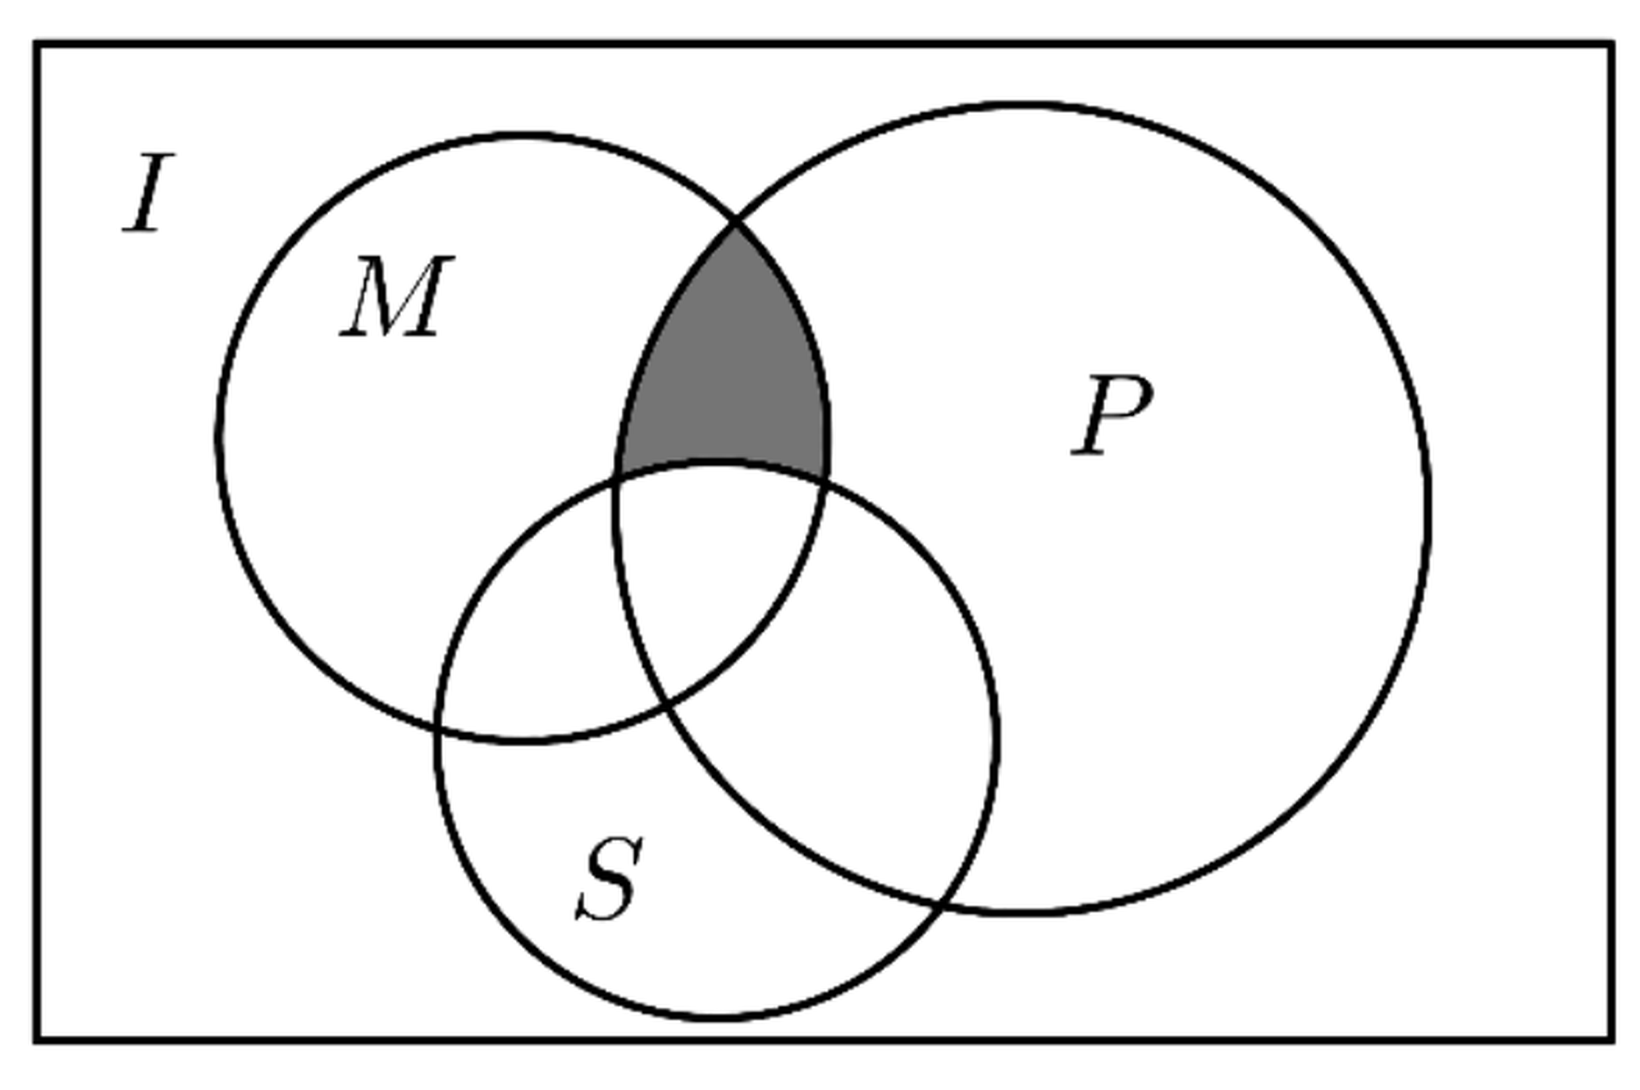
\includegraphics[width=0.42\textwidth]{figures/gao120_q15.png}
\end{center}

\keepwithprev
A. $(M\cap P)\cap S$\qquad\quad B. $(M\cap P)\cap\complement_{I}S$\qquad\quad C. $(M\cup P)\cap S$\qquad\quad D. $\complement_{I}(M\cap P)\cap S$

\ifanswer
\solbegin
\step{由已知中的 $Venn$ 图得阴影部分的元素属于 $M$，属于 $P$，但不属于 $S$，}
\step{所以阴影部分表示的集合为 $(M\cap P)\cap\complement_{I}S$，故选 $B$.}
\solend
\fi

\item 设集合 $P_1=\{x\mid x^2+ax+1>0\}$，$P_2=\{x\mid x^2+ax+2>0\}$，$Q_1=\{x\mid x^2+x+b>0\}$，$Q_2=\{x\mid x^2+2x+b>0\}$，其中 $a$、$b\in\R$，对于下列两个命题：①存在 $a$，$P_1$ 不是 $P_2$ 的子集；②存在 $b$ 使得 $Q_1$ 是 $Q_2$ 的子集. 下列说法正确的是\mbox{（\quad）}

\keepwithprev
A. ①是真命题，②是假命题\qquad\qquad B. ①是假命题，②是真命题

C. ①②都是真命题\qquad\qquad\qquad D. ①②都是假命题

\ifanswer
\solbegin
\step{对于集合 $P_1=\{x\mid x^2+ax+1>0\}$，$P_2=\{x\mid x^2+ax+2>0\}$，}
\step{得当 $m\in P_1$ 时，即 $m^2+am+1>0$，得 $m^2+am+2>0$，}
\step{即有 $m\in P_2$，得对任意 $a$，$P_1$ 是 $P_2$ 的子集，故①错误；}
\step{对于集合 $Q_1=\{x\mid x^2+x+b>0\}$，$Q_2=\{x\mid x^2+2x+b>0\}$，}
\step{当 $b=6$ 时，$Q_1=\{x\mid x^2+x+6>0\}=\R$，$Q_2=\{x\mid x^2+2x+6>0\}=\R$，}
\step{得 $Q_1$ 是 $Q_2$ 的子集，所以存在 $b$，使得 $Q_1$ 是 $Q_2$ 的子集，故②正确；}
\step{故选 $B$.}
\solend
\fi

\end{enumerate}

\bigsec{三、解答题}

\begin{enumerate}
\setcounter{enumi}{16}

\item (1) 已知 $x$、$y$ 都是实数，比较 $x^2+y^2$ 与 $4x-2y-5$ 的大小.

(2) 求解不等式组 $\begin{cases}x^2-4x+3\geqslant0\\\dfrac{x+3}{2x-1}\geqslant2\end{cases}$.

\ifanswer
\solbegin
\step{(1) $(x^2+y^2)-(4x-2y-5)=x^2-4x+y^2+2y+5=(x-2)^2+(y+1)^2\geqslant0$，}
\step{当 $x=2$，$y=-1$ 时，$x^2+y^2=4x-2y-5$.}
\step{当 $x\neq2$ 或 $y\neq-1$ 时，$x^2+y^2>4x-2y-5$.}
\step{(2) 由 $x^2-4x+3\geqslant0$ 得 $(x-1)(x-3)\geqslant0$，所以 $x\leqslant1$ 或 $x\geqslant3$；}
\step{由 $\dfrac{x+3}{2x-1}\geqslant2$，得 $\dfrac{x+3}{2x-1}-2=\dfrac{-3x+5}{2x-1}\geqslant0$，即 $\dfrac{3x-5}{2x-1}\leqslant0$，}
\step{所以 $\begin{cases}(3x-5)(2x-1)\leqslant0\\2x-1\neq0\end{cases}$，解得 $\dfrac12<x\leqslant\dfrac53$，}
\step{所以不等式组的解集是 $\left\{x\,\middle\vert\,\dfrac12<x\leqslant1\right\}$.}
\solend
\fi

\item 已知 $x_1$,$x_2$ 是一元二次方程 $4kx^2-4kx+k+1=0$ 的两个实数根.

(1) 是否存在实数 $k$，$(2x_1-x_2)(x_1-2x_2)=-\dfrac32$ 成立？若存在，求出 $k$ 的值；若不存在，请说明理由.

(2) 求使 $\dfrac{x_1}{x_2}+\dfrac{x_2}{x_1}-2$ 的值为整数的实数 $k$ 的整数值.

\ifanswer
\solbegin
\step{(1) 因为 $x_1$,$x_2$ 是一元二次方程 $4kx^2-4kx+k+1=0$ 的两个实数根，}
\step{所以 $\begin{cases}k\neq0\\16k^2-16k(k+1)\geqslant0\end{cases}$，所以 $k<0$，}
\step{由根与系数的关系得 $x_1+x_2=1$，$x_1x_2=\dfrac{k+1}{4k}$，}
\step{所以 $(2x_1-x_2)(x_1-2x_2)=2(x_1+x_2)^2-9x_1x_2=2-9\times\dfrac{k+1}{4k}=-\dfrac32$，}
\step{解得 $k=\dfrac95$，而 $k<0$，故不存在实数 $k$ 使得 $(2x_1-x_2)(x_1-2x_2)=-\dfrac32$ 成立.}
\step{(2) 由根与系数的关系得 $\dfrac{x_1}{x_2}+\dfrac{x_2}{x_1}-2=\dfrac{(x_1+x_2)^2}{x_1x_2}-4=-\dfrac4{k+1}$，}
\step{因为 $-\dfrac4{k+1}$ 的值为整数，而 $k$ 为整数，所以 $k+1$ 只能取 $\pm1$、$\pm2$、$\pm4$，}
\step{又 $k<0$，所以整数 $k$ 的值为 $-2$ 或 $-3$ 或 $-5$.}
\solend
\fi

\item 2026 年，某市低空经济蓬勃发展，一家物流企业开通“无人机即时配送”服务，并设立配送站. 经市场调研，该站每日配送单量 $y$（单位：单）与每单配送费 $x$（单位：元）满足关系式 $y=4800-200x$（其中 $4<x<24$）. 已知配送站每日的固定成本为 $19200$ 元，每完成一单配送，需支付电费、耗材费、设备保养费等可变成本，每单可变成本为 $4$ 元.

(1) 若要保证配送站每日利润 $W$（单位：元）不为负数，求每单配送费 $x$ 的取值范围；（每日利润 $=$ 每日配送总收入 $-$ 每日可变总成本 $-$ 每日固定成本）

(2) 为提升运力，该站购进一批新型无人机，购机费用为 $32$ 万元. 投入使用后，这批无人机使用 $t(t>0)$ 年的累计维保总费用为 $(2t^2+8t)$ 万元. 请问：这批无人机使用多少年后更新，可以使年平均总费用最低？请求出最低年平均总费用.（年平均总费用 $=$（购机费用 $+$ 维保总费用）$\div$ 使用年数）

\ifanswer
\solbegin
\step{(1) $W=xy-4y-19200=x(4800-200x)-4(4800-200x)-19200$}
\step{$=-200x^2+5600x-38400(4<x<24)$，}
\step{令 $W=-200x^2+5600x-38400\geqslant0$，即 $x^2-28x+192\leqslant0$，}
\step{解得 $12\leqslant x\leqslant16$，因此，要保证配送站每日利润 $W$ 不为负数，}
\step{每单配送费 $x$ 的取值范围为 $[12,16]$；}
\step{(2) 由题意，年平均总费用为 $N=\dfrac{2t^2+8t+32}{t}=2t+\dfrac{32}{t}+8$}
\step{$\geqslant2\sqrt{2t\cdot\dfrac{32}{t}}+8=16+8=24$，当且仅当 $2t=\dfrac{32}{t}$，即 $t=4$ 时取等号，}
\step{则这批无人机使用 $4$ 年后更新，可以使年平均总费用最低，}
\step{最低年平均总费用为 $24$ 万元.}
\solend
\fi

\item 已知 $A,B$，定义集合 $M_{(A,B)}=\{x\mid A<B\}$.

(1) 设 $A=\lvert x-4\rvert$,$B=2x$，求 $M_{(A,B)}$；

(2) 设 $A=ax^2+2ax-4$,$B=2x(x+2)$，当 $M_{(A,B)}=\R$ 时，求 $a$ 的取值范围；

(3) 设 $A=\lvert 2x-b\rvert$,$B=\dfrac{x+4b}{x-1}$,$C=2$，若 $M_{(A,C)}\cap M_{(B,C)}\neq\varnothing$，求 $b$ 的取值范围.

\ifanswer
\solbegin
\step{(1) 由定义，$x\in M_{(A,B)}$ 等价于 $\lvert x-4\rvert<2x$，}
\step{原不等式等价于 $-2x<x-4<2x$，即同时满足 $3x>4$ 与 $x>-4$，}
\step{解得 $x>\dfrac43$，所以 $M_{(A,B)}=\left(\dfrac43,+\infty\right)$.}
\step{(2) 由 $M_{(A,B)}=\R$，得 $ax^2+2ax-4<2x(x+2)$ 对任意 $x\in\R$ 恒成立，}
\step{得 $(a-2)(x+1)^2-a-2<0$.}
\step{当 $a>2$ 时，随着 $(x+1)^2$ 增大，左边可取正值，不符合题意；}
\step{当 $a=2$ 时，左边恒等于 $-4$，符合题意；}
\step{当 $a<2$ 时，左边在 $x=-1$ 处取得最大值 $-a-2$，}
\step{故恒成立的充要条件为 $-a-2<0$，即 $a>-2$；}
\step{综上，$a\in(-2,2]$.}
\step{(3) 由 $\lvert 2x-b\rvert<2$，得 $M_{(A,C)}=\left(\dfrac b2-1,\dfrac b2+1\right)$，记为 $I$.}
\step{由 $\dfrac{x+4b}{x-1}<2$，得 $\dfrac{x-(4b+2)}{x-1}>0$，其中 $x\neq1$.}
\step{①当 $b<-\dfrac14$ 时，$4b+2<1$，故 $M_{(B,C)}=(-\infty,4b+2)\cup(1,+\infty)$.}
\step{此时 $\dfrac b2+1<1$，所以 $I$ 与 $(1,+\infty)$ 没有公共元素.}
\step{两集合交集非空等价于 $\dfrac b2-1<4b+2$，解得 $b>-\dfrac67$.}
\step{因而本种情况得到 $-\dfrac67<b<-\dfrac14$.}
\step{②当 $b=-\dfrac14$ 时，$\dfrac{x+4b}{x-1}=1$，其中 $x\neq1$，故 $M_{(B,C)}=\{x\mid x\neq1\}$.}
\step{此时 $I=\left(-\dfrac98,\dfrac78\right)$，两集合交集非空.}
\step{③当 $b>-\dfrac14$ 时，$4b+2>1$，故 $M_{(B,C)}=(-\infty,1)\cup(4b+2,+\infty)$.}
\step{此时 $4b+2-\left(\dfrac b2+1\right)=\dfrac{7b}{2}+1>\dfrac18>0$，}
\step{所以 $I$ 与 $(4b+2,+\infty)$ 没有公共元素.}
\step{两集合交集非空等价于 $\dfrac b2-1<1$，解得 $b<4$.}
\step{因而本种情况得到 $-\dfrac14<b<4$.}
\step{综上，$b\in\left(-\dfrac67,4\right)$.}
\solend
\fi

\item 破晓同学阅读课外书籍时，发现笛卡尔积是代数和图论中一个很重要的课题. 对于非空数集 $A,B$，定义 $A\otimes B=\{(x,y)\mid x\in A$ 且 $y\in B\}$，将 $A\otimes B$ 称为“$A$ 与 $B$ 的笛卡尔积”.

(1) 若 $A=\{-1,0,1\}$,$B=\{-1,1\}$，求 $A\otimes B$ 和 $B\otimes A$；

(2) 试证明：“$A_1\otimes A_2=A_2\otimes A_1$”是“$A_1=A_2$”的充要条件；

(3) 若集合 $H$ 是有限集，将集合 $H$ 的元素个数记为 $\lvert H\rvert$. 已知 $\lvert A_1\otimes A_2\rvert=m^3(m\in\N^*)$，且存在实数 $a$ 满足 $\sqrt{\dfrac{\lvert A_1\otimes A_1\rvert+\lvert A_2\otimes A_2\rvert}{\lvert A_2\otimes A_1\rvert}}\geqslant a$ 对任意 $m\in\N^*$ 恒成立. 求 $a$ 的取值范围，并指明当 $a$ 取到最值时 $\lvert A_1\rvert$ 和 $\lvert A_2\rvert$ 满足的关系式及 $m$ 应满足的条件.

\ifanswer
\solbegin
\step{(1) 由题意得 $A\otimes B=\{(-1,-1),(-1,1),(0,-1),(0,1),(1,-1),(1,1)\}$，}
\step{$B\otimes A=\{(-1,-1),(-1,0),(-1,1),(1,-1),(1,0),(1,1)\}$；}
\step{(2) 若 $A_1=A_2$，设 $A_1=A_2=A$，}
\step{由定义得 $A_1\otimes A_2=\{(a,b)\mid a\in A$ 且 $b\in A\}=A_2\otimes A_1$，}
\step{所以“$A_1\otimes A_2=A_2\otimes A_1$”是“$A_1=A_2$”的必要条件；}
\step{若 $A_1\otimes A_2=A_2\otimes A_1$，对任意 $(a,b)\in A_1\otimes A_2$，均有 $(a,b)\in A_2\otimes A_1$，}
\step{即对任意 $a\in A_1,b\in A_2$，均有 $a\in A_2,b\in A_1$，}
\step{由任意性得 $A_1\subseteq A_2,A_2\subseteq A_1$，则 $A_1=A_2$，}
\step{所以“$A_1\otimes A_2=A_2\otimes A_1$”是“$A_1=A_2$”的充分条件；}
\step{综上所述，“$A_1\otimes A_2=A_2\otimes A_1$”是“$A_1=A_2$”的充要条件.}
\step{(3) 设 $\lvert A_1\rvert=c$,$\lvert A_2\rvert=d$,$c,d\in\N^*$，}
\step{则 $\lvert A_1\otimes A_2\rvert=\lvert A_2\otimes A_1\rvert=cd=m^3$,$\lvert A_1\otimes A_1\rvert=c^2$,$\lvert A_2\otimes A_2\rvert=d^2$，}
\step{得 $\sqrt{\dfrac{\lvert A_1\otimes A_1\rvert+\lvert A_2\otimes A_2\rvert}{\lvert A_2\otimes A_1\rvert}}=\sqrt{\dfrac{c^2+d^2}{cd}}=\sqrt{\dfrac cd+\dfrac dc}\geqslant\sqrt{2\sqrt{\dfrac cd\cdot\dfrac dc}}=\sqrt2$，}
\step{当且仅当 $\dfrac cd=\dfrac dc$，即 $c=d$ 时取等号，所以实数 $a$ 的取值范围是 $(-\infty,\sqrt2]$.}
\step{若 $a$ 取到最大值，则 $c=d$，即 $\lvert A_1\rvert=\lvert A_2\rvert$，得 $c^2=m^3$，}
\step{即 $c=\sqrt{m^3}=(\sqrt m)^3\in\N^*$，所以 $m=k^2,k\in\N^*$.}
\solend
\fi

\end{enumerate}

\end{document}
"
% 紧凑版：xelatex "\def\iscompact{1}% 高一120_松江二中_10月月考.tex
%   —— 高一上数学“2026-2027 年松江二中高一上 10 月月考”（试卷版/答案版）
% 试卷版：xelatex 高一120_松江二中_10月月考.tex
% 答案版：xelatex "\def\isanswer{1}% 高一120_松江二中_10月月考.tex
%   —— 高一上数学“2026-2027 年松江二中高一上 10 月月考”（试卷版/答案版）
% 试卷版：xelatex 高一120_松江二中_10月月考.tex
% 答案版：xelatex "\def\isanswer{1}% 高一120_松江二中_10月月考.tex
%   —— 高一上数学“2026-2027 年松江二中高一上 10 月月考”（试卷版/答案版）
% 试卷版：xelatex 高一120_松江二中_10月月考.tex
% 答案版：xelatex "\def\isanswer{1}\input{高一120_松江二中_10月月考.tex}"
% 紧凑版：xelatex "\def\iscompact{1}\input{高一120_松江二中_10月月考.tex}"
%
% 原始材料：微信公众号“魔都数学加油站”文章，作者破晓，2026-11-08 21:35 发布；
% 连载“27学年高一120”，原文标题“27学年高一120——2026-2027年上海市松江二中高一上10月月考”；
% 原文链接：https://mp.weixin.qq.com/s/hgDkaZX9M_IKhmr7CjQc1A。
% 正文为 10 张 PNG 页（第 8、10 页 2560×3620，其余 4762×6735），
% 题目下印有【解析】或【答案】，为讲评版。
% 题目、解析均据原图转录；卷面红色水印及公众号页脚未录入。
% 全卷 1 张插图：第 15 题的三集合 Venn 图（原卷印在题干右侧，本稿移至题干之后，
% 取原卷截图 2× LANCZOS 放大，见 figures/gao120_q15.png）。
%
% 卷首标题：原卷印作“2026-2027 年松江二中高一上 10 月月考”（公众号标题中的“上海市”
% 卷面标题行没有，本稿照卷面），年份区间按全稿惯例排 en dash；原卷未印副标题，本稿按题目内容
% 标为“集合与常用逻辑用语、不等式”（与 110／111／113／116／118 同）。
%
% 与原卷的排版差异：
%   ① 原文从第 3 题起，填空题编号为 3—12、选择题为 13—16、解答题为 17—21，本稿保留原题号；
%   ② 原卷每题下直接印【解析】／【答案】，本稿按全稿惯例置于答案版；第 3 题只印【答案】、
%      第 13、14 题把答案印在题干括号内且无【解析】，均另提 \ans{}；其余选择题答案在
%      解析末句“故选 …”，括号内留空；
%   ③ 原卷未印副标题，本稿按“知识模块”口径补出；
%   ④ 原卷填空横线按全稿惯例排为 \blankline[4.4em]；选择题括号排 \mbox{（\quad）}、
%      选项段前按惯例加 \keepwithprev；解答题不留作答区（原卷为讲评版，与 109—119 同）；
%   ⑤ 原卷数集排斜体 $R$、$N^*$，按全稿惯例改 \R、\N^*；绝对值排 \lvert…\rvert，
%      集合描述竖线排 \mid；补集记号照原卷排 \complement_I。
%
% 判别式字形：第 9 题解析作 $\triangle$（等边、扁），照录 \triangle。
%
% 子集符号：第 4 题题干与解析的 $A\subseteq B$、第 21 题 (2) 的 $A_1\subseteq A_2$ 印有下划线，
%   照录 \subseteq。
%
% 原卷存疑照录：第 12 题题干 $S=\{82,83,84,85,86,87,89\}$ 跳过 $88$ 只列 7 个数，
%   与其“8 种不同的值”自洽（不含 $88$），照录；第 19 题 (1) 的 $W$ 表达式
%   $x(4800-200x)-4(4800-200x)-19200$ 与最后结果 $[12,16]$ 一致。
%
% 行数核对：逐题数 \step 条数，合计 115 条（Q3：0；Q4：4；Q5：2；Q6：5；Q7：4；
% Q8：2；Q9：5；Q10：3；Q11：6；Q12：11；Q13：0；Q14：0；Q15：2；Q16：7；
% Q17：7；Q18：8；Q19：9；Q20：24；Q21：16），与原卷印刷行逐题相等
% （cases 块作一个印刷行计）。第 3 题只印【答案】、第 13、14 题括号内印答案且无解析，
% 均提 \ans{}，不计入 \step 账。
%
\documentclass[a4paper,11pt]{article}
\usepackage{common}

\begin{document}

\examtitlest[3]{2026--2027 年松江二中高一上 10 月月考}{集合与常用逻辑用语、不等式}

\bigsec{一、填空题}

\begin{enumerate}
\setcounter{enumi}{2}

\item 集合 $A=\{(x,y)\mid x+y=8\}$,$B=\{(x,y)\mid xy=12\}$，求 $A\cap B=$\blankline[4.4em].

\ifanswer
\ans{$\{(2,6),(6,2)\}$}
\fi

\item 设集合 $A=\{0,-a\}$,$B=\{1,a-2,2a-2\}$，若 $A\subseteq B$，则 $a=$\blankline[4.4em].

\ifanswer
\solbegin
\step{因为 $A\subseteq B$，}
\step{若 $a-2=0$，解得 $a=2$，此时 $A=\{0,-2\}$,$B=\{1,0,2\}$，不符合题意；}
\step{若 $2a-2=0$，解得 $a=1$，此时 $A=\{0,-1\}$,$B=\{1,-1,0\}$，符合题意；}
\step{综上所述，$a=1$.}
\solend
\fi

\item 设 $\alpha:0<x<a(a>0)$,$\beta:x<8-3a$，若 $\alpha$ 是 $\beta$ 的充分条件，则实数 $a$ 的取值范围是\blankline[4.4em].

\ifanswer
\solbegin
\step{由 $\alpha$ 是 $\beta$ 的充分条件得，$x\in(0,a)\Rightarrow x\in(-\infty,8-3a)$，}
\step{所以 $0<a\leqslant8-3a$，解得 $0<a\leqslant2$.}
\solend
\fi

\item 关于 $x$ 的不等式 $ax-b>0$ 的解集为 $(-\infty,1)$，则不等式 $\dfrac{x-2}{ax+b}<0$ 的解集为\blankline[4.4em].

\ifanswer
\solbegin
\step{因为关于 $x$ 的不等式 $ax-b>0$ 的解集为 $(-\infty,1)$，}
\step{所以 $a<0$ 且 $\dfrac ba=1$，则 $b=a$，}
\step{所以不等式 $\dfrac{x-2}{ax+b}<0$，即 $\dfrac{x-2}{ax+a}<0$，即 $\dfrac{x-2}{x+1}>0$，}
\step{等价于 $(x+1)(x-2)>0$，解得 $x>2$ 或 $x<-1$，}
\step{即解集为 $(-\infty,-1)\cup(2,+\infty)$.}
\solend
\fi

\item 若正实数 $x$、$y$ 满足 $2x+y+8xy=2$，则 $xy$ 的最大值为\blankline[4.4em].

\ifanswer
\solbegin
\step{因为正实数 $x$、$y$ 满足 $2x+y+8xy=2$，}
\step{所以 $2-8xy=2x+y\geqslant2\sqrt{2xy}$，}
\step{当且仅当 $y=2x$，即 $x=\dfrac14$，$y=\dfrac12$ 时取等号，解得 $0<xy\leqslant\dfrac18$，}
\step{故 $xy$ 的最大值为 $\dfrac18$.}
\solend
\fi

\item 已知 $1<a<3$，$-5<b<-2$，则 $\dfrac ab$ 的取值范围是\blankline[4.4em].

\ifanswer
\solbegin
\step{因为 $-5<b<-2$，所以 $2<-b<5$，$\dfrac15<-\dfrac1b<\dfrac12$，又 $1<a<3$，}
\step{得 $\dfrac15<-\dfrac ab<\dfrac32$，则 $-\dfrac32<\dfrac ab<-\dfrac15$，故 $\dfrac ab$ 的取值范围是 $\left(-\dfrac32,-\dfrac15\right)$.}
\solend
\fi

\item 若关于 $x$、$y$ 的方程组 $\begin{cases}y-kx-2=0\\y^2-4x-2y+1=0\end{cases}$ 的解集中只有一个元素，则实数 $k$ 的值为\blankline[4.4em].

\ifanswer
\solbegin
\step{由 $\begin{cases}y-kx-2=0\\y^2-4x-2y+1=0\end{cases}$ 消去 $y$ 整理得 $k^2x^2+(2k-4)x+1=0$.}
\step{当 $k\neq0$ 时，则 $\triangle=(2k-4)^2-4k^2=0$，解得 $k=1$，}
\step{此时方程组的解为 $\begin{cases}x=1\\y=3\end{cases}$，符合题意；}
\step{当 $k=0$ 时，解得 $x=\dfrac14$，此时方程组的解为 $\begin{cases}x=\dfrac14\\y=2\end{cases}$，符合题意；}
\step{综上，$k=0$ 或 $k=1$.}
\solend
\fi

\item 若集合 $A=\{0,1\}$，$B=\{x\mid x^2-mx-m>0,x\in\R\}$，且 $A\cap B=\{1\}$，则实数 $m$ 的取值范围为\blankline[4.4em].

\ifanswer
\solbegin
\step{因为集合 $A=\{0,1\}$，$B=\{x\mid x^2-mx-m>0,x\in\R\}$，且 $A\cap B=\{1\}$，}
\step{则 $1\in B$ 且 $0\notin B$，所以 $\begin{cases}1-m-m>0\\-m\leqslant0\end{cases}$，解得 $0\leqslant m<\dfrac12$，}
\step{所以实数 $m$ 的取值范围是 $\left[0,\dfrac12\right)$.}
\solend
\fi

\item 从集合 $U=\{a,b,c,d\}$ 的子集中选出两个不同的子集，需同时满足以下两个条件：(1) $a$、$b$ 都至少属于其中一个集合；(2) 对选出的两个子集，其中一个集合为另一个的子集，那么共有\blankline[4.4em]种不同的选法.

\ifanswer
\solbegin
\step{不妨设元素少的为 $A$，元素多的为 $B$，则 $B$ 必包含有 $a$、$b$；$A$ 为 $B$ 的真子集，}
\step{若 $B=\{a,b\}$，$A$ 为 $B$ 的真子集，共 $2^2-1=3$ 种，}
\step{若 $B=\{a,b,c\}$，$A$ 为 $B$ 的真子集，共 $2^3-1=7$ 种，}
\step{若 $B=\{a,b,d\}$，$A$ 为 $B$ 的真子集，共 $2^3-1=7$ 种，}
\step{若 $B=\{a,b,c,d\}$，$A$ 为 $B$ 的真子集，共 $2^4-1=15$ 种，}
\step{共有 $3+7+7+15=32$ 种.}
\solend
\fi

\item 已知 $a_1$、$a_2$、$\cdots$、$a_8$ 是 $8$ 个正整数，记 $S=\{a_{i_1}+a_{i_2}+\cdots+a_{i_7}\mid 1\leqslant i_1<i_2<\cdots<i_7\leqslant8\}$，其中 $i_1$、$i_2$、$\cdots$、$i_7\in\N^*$，若 $S=\{82,83,84,85,86,87,89\}$，则这 $8$ 个正整数中的最大数与最小数的积为\blankline[4.4em].

\ifanswer
\solbegin
\step{由题意得从 $8$ 个数中任取 $7$ 个数的和共有 $C_8^7=8$ 种不同的值，}
\step{但是 $82$，$83$，$84$，$85$，$86$，$87$，$89$ 只有 $7$ 个数，}
\step{得必有两种 $7$ 个数的和相等，设这个和为 $t(82\leqslant t\leqslant89)$，}
\step{令 $T=\sum\limits_{i=1}^{8}a_i$，那么，任取 $7$ 个数的和就等于 $T-a_i$，$i=1,2,\cdots,8$，}
\step{这 $8$ 个取值和的集合为 $S$，$S=\{T-a_1,T-a_2,\cdots,T-a_8\}$，}
\step{则 $\sum\limits_{i=1}^{8}(T-a_i)=8T-T=7T=82+83+84+85+86+87+89+t=596+t$.}
\step{因为 $T$ 为整数，所以 $596+t$ 是 $7$ 的倍数，}
\step{由 $596=7\times85+1$ 得 $1+t$ 是 $7$ 的倍数，}
\step{再因为 $82\leqslant t\leqslant89$，所以 $t=83$，得 $T=97$.}
\step{因此 $a_1$、$a_2$、$\cdots$、$a_8$ 中最大数为 $97-82=15$，最小数为 $97-89=8$，}
\step{因此，它们的积为 $120$.}
\solend
\fi

\end{enumerate}

\bigsec{二、选择题}

\begin{enumerate}
\setcounter{enumi}{12}

\item 已知 $a>b>0$，$c\in\R$，则下列不等式不一定成立的是\mbox{（\quad）}% 原卷把答案“$B$”印在题干括号内、无【解析】

\keepwithprev
A. $a-c>b-c$\qquad\quad B. $ac>bc$\qquad\quad C. $\dfrac1a<\dfrac1b$\qquad\quad D. $\dfrac{a+b}{2}>\sqrt{ab}$

\ifanswer
\ans{$B$}
\fi

\item 命题“对任意的 $x\in\R,x^3-x^2+1\leqslant0$”的否定是\mbox{（\quad）}% 原卷把答案“$C$”印在题干括号内、无【解析】

\keepwithprev
A. 不存在 $x\in\R,x^3-x^2+1\leqslant0$\qquad B. 存在 $x\in\R,x^3-x^2+1\leqslant0$

C. 存在 $x\in\R,x^3-x^2+1>0$\qquad\quad D. 对任意的 $x\in\R,x^3-x^2+1>0$

\ifanswer
\ans{$C$}
\fi

% 第 15 题是“题干 + 图 + 选项”约 6.5cm 的一整块，\keepwithprev 只挡得住“图—选项”，
% 挡不住夹在中间的图——实测断点落在题干之后（切页审计 A 类）。故照 高一30／高一26 成例
% 在题前先量一次页高，不够就把整块一起挪到次页。
\needvspace{7cm}
\item 如图，$I$ 是全集，$M$、$P$、$S$ 是 $I$ 的三个子集，则阴影部分所表示的集合是\mbox{（\quad）}

\begin{center}
% 图取原卷截图（第 4 页题干右侧）、2× LANCZOS 放大，本稿移至题干之后
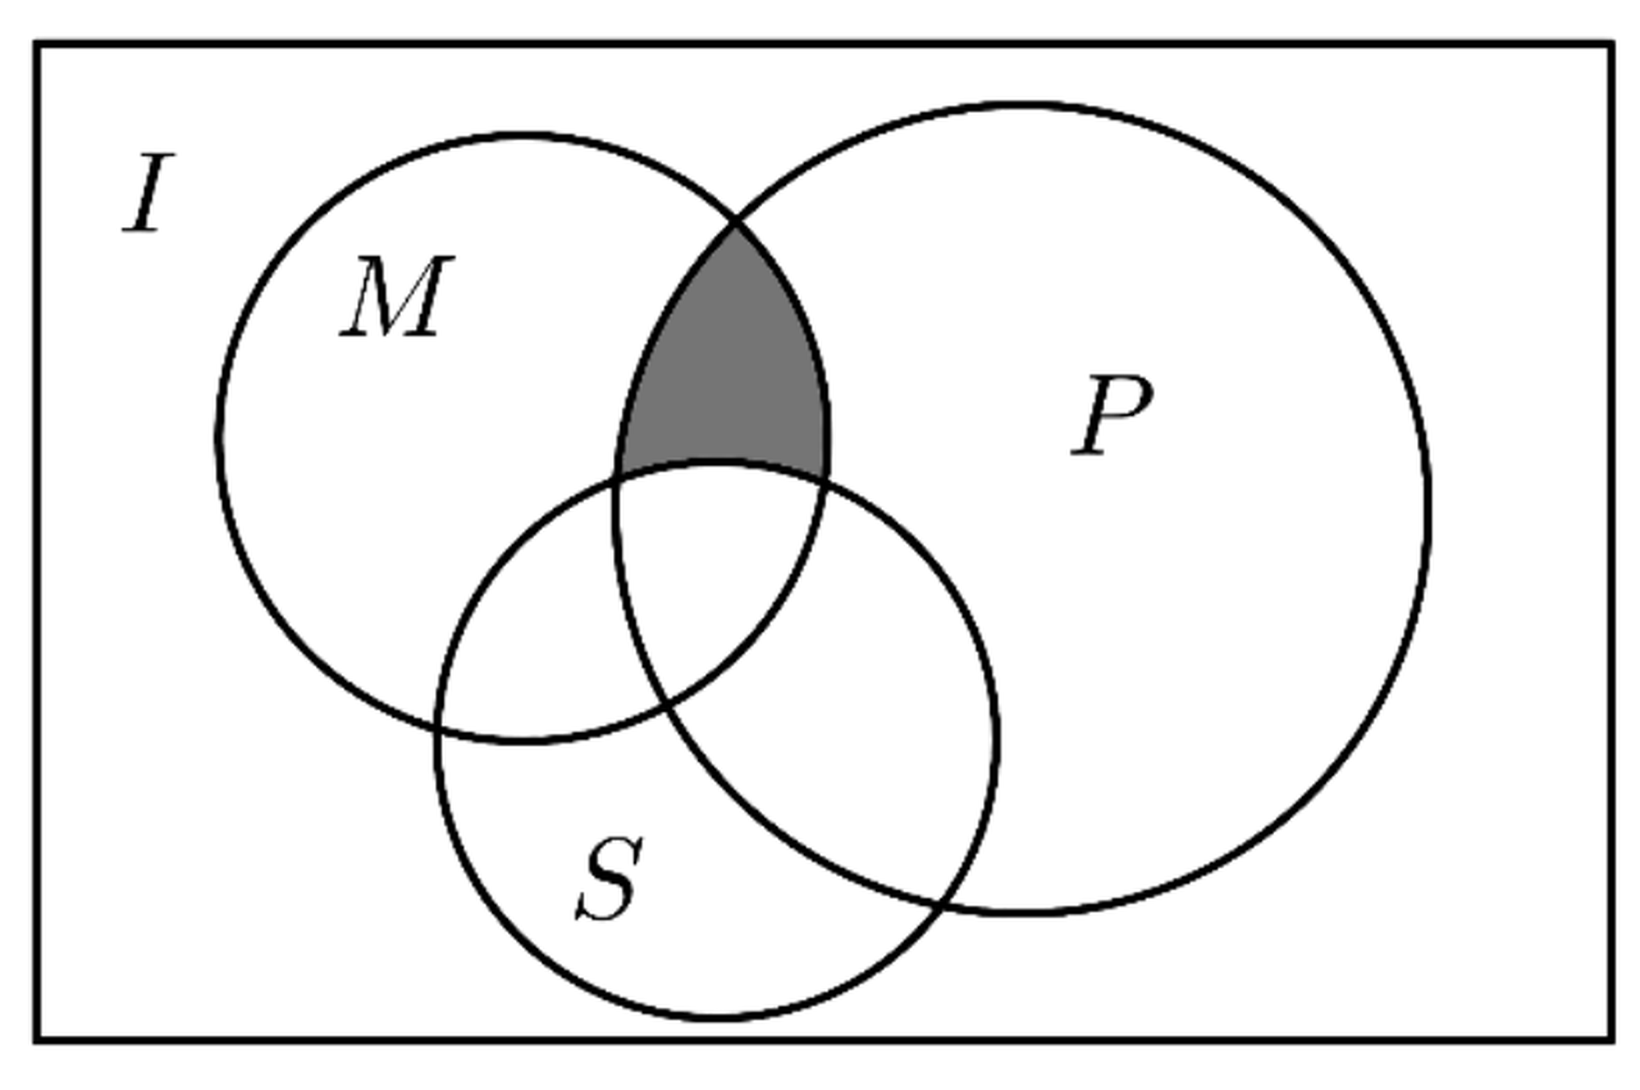
\includegraphics[width=0.42\textwidth]{figures/gao120_q15.png}
\end{center}

\keepwithprev
A. $(M\cap P)\cap S$\qquad\quad B. $(M\cap P)\cap\complement_{I}S$\qquad\quad C. $(M\cup P)\cap S$\qquad\quad D. $\complement_{I}(M\cap P)\cap S$

\ifanswer
\solbegin
\step{由已知中的 $Venn$ 图得阴影部分的元素属于 $M$，属于 $P$，但不属于 $S$，}
\step{所以阴影部分表示的集合为 $(M\cap P)\cap\complement_{I}S$，故选 $B$.}
\solend
\fi

\item 设集合 $P_1=\{x\mid x^2+ax+1>0\}$，$P_2=\{x\mid x^2+ax+2>0\}$，$Q_1=\{x\mid x^2+x+b>0\}$，$Q_2=\{x\mid x^2+2x+b>0\}$，其中 $a$、$b\in\R$，对于下列两个命题：①存在 $a$，$P_1$ 不是 $P_2$ 的子集；②存在 $b$ 使得 $Q_1$ 是 $Q_2$ 的子集. 下列说法正确的是\mbox{（\quad）}

\keepwithprev
A. ①是真命题，②是假命题\qquad\qquad B. ①是假命题，②是真命题

C. ①②都是真命题\qquad\qquad\qquad D. ①②都是假命题

\ifanswer
\solbegin
\step{对于集合 $P_1=\{x\mid x^2+ax+1>0\}$，$P_2=\{x\mid x^2+ax+2>0\}$，}
\step{得当 $m\in P_1$ 时，即 $m^2+am+1>0$，得 $m^2+am+2>0$，}
\step{即有 $m\in P_2$，得对任意 $a$，$P_1$ 是 $P_2$ 的子集，故①错误；}
\step{对于集合 $Q_1=\{x\mid x^2+x+b>0\}$，$Q_2=\{x\mid x^2+2x+b>0\}$，}
\step{当 $b=6$ 时，$Q_1=\{x\mid x^2+x+6>0\}=\R$，$Q_2=\{x\mid x^2+2x+6>0\}=\R$，}
\step{得 $Q_1$ 是 $Q_2$ 的子集，所以存在 $b$，使得 $Q_1$ 是 $Q_2$ 的子集，故②正确；}
\step{故选 $B$.}
\solend
\fi

\end{enumerate}

\bigsec{三、解答题}

\begin{enumerate}
\setcounter{enumi}{16}

\item (1) 已知 $x$、$y$ 都是实数，比较 $x^2+y^2$ 与 $4x-2y-5$ 的大小.

(2) 求解不等式组 $\begin{cases}x^2-4x+3\geqslant0\\\dfrac{x+3}{2x-1}\geqslant2\end{cases}$.

\ifanswer
\solbegin
\step{(1) $(x^2+y^2)-(4x-2y-5)=x^2-4x+y^2+2y+5=(x-2)^2+(y+1)^2\geqslant0$，}
\step{当 $x=2$，$y=-1$ 时，$x^2+y^2=4x-2y-5$.}
\step{当 $x\neq2$ 或 $y\neq-1$ 时，$x^2+y^2>4x-2y-5$.}
\step{(2) 由 $x^2-4x+3\geqslant0$ 得 $(x-1)(x-3)\geqslant0$，所以 $x\leqslant1$ 或 $x\geqslant3$；}
\step{由 $\dfrac{x+3}{2x-1}\geqslant2$，得 $\dfrac{x+3}{2x-1}-2=\dfrac{-3x+5}{2x-1}\geqslant0$，即 $\dfrac{3x-5}{2x-1}\leqslant0$，}
\step{所以 $\begin{cases}(3x-5)(2x-1)\leqslant0\\2x-1\neq0\end{cases}$，解得 $\dfrac12<x\leqslant\dfrac53$，}
\step{所以不等式组的解集是 $\left\{x\,\middle\vert\,\dfrac12<x\leqslant1\right\}$.}
\solend
\fi

\item 已知 $x_1$,$x_2$ 是一元二次方程 $4kx^2-4kx+k+1=0$ 的两个实数根.

(1) 是否存在实数 $k$，$(2x_1-x_2)(x_1-2x_2)=-\dfrac32$ 成立？若存在，求出 $k$ 的值；若不存在，请说明理由.

(2) 求使 $\dfrac{x_1}{x_2}+\dfrac{x_2}{x_1}-2$ 的值为整数的实数 $k$ 的整数值.

\ifanswer
\solbegin
\step{(1) 因为 $x_1$,$x_2$ 是一元二次方程 $4kx^2-4kx+k+1=0$ 的两个实数根，}
\step{所以 $\begin{cases}k\neq0\\16k^2-16k(k+1)\geqslant0\end{cases}$，所以 $k<0$，}
\step{由根与系数的关系得 $x_1+x_2=1$，$x_1x_2=\dfrac{k+1}{4k}$，}
\step{所以 $(2x_1-x_2)(x_1-2x_2)=2(x_1+x_2)^2-9x_1x_2=2-9\times\dfrac{k+1}{4k}=-\dfrac32$，}
\step{解得 $k=\dfrac95$，而 $k<0$，故不存在实数 $k$ 使得 $(2x_1-x_2)(x_1-2x_2)=-\dfrac32$ 成立.}
\step{(2) 由根与系数的关系得 $\dfrac{x_1}{x_2}+\dfrac{x_2}{x_1}-2=\dfrac{(x_1+x_2)^2}{x_1x_2}-4=-\dfrac4{k+1}$，}
\step{因为 $-\dfrac4{k+1}$ 的值为整数，而 $k$ 为整数，所以 $k+1$ 只能取 $\pm1$、$\pm2$、$\pm4$，}
\step{又 $k<0$，所以整数 $k$ 的值为 $-2$ 或 $-3$ 或 $-5$.}
\solend
\fi

\item 2026 年，某市低空经济蓬勃发展，一家物流企业开通“无人机即时配送”服务，并设立配送站. 经市场调研，该站每日配送单量 $y$（单位：单）与每单配送费 $x$（单位：元）满足关系式 $y=4800-200x$（其中 $4<x<24$）. 已知配送站每日的固定成本为 $19200$ 元，每完成一单配送，需支付电费、耗材费、设备保养费等可变成本，每单可变成本为 $4$ 元.

(1) 若要保证配送站每日利润 $W$（单位：元）不为负数，求每单配送费 $x$ 的取值范围；（每日利润 $=$ 每日配送总收入 $-$ 每日可变总成本 $-$ 每日固定成本）

(2) 为提升运力，该站购进一批新型无人机，购机费用为 $32$ 万元. 投入使用后，这批无人机使用 $t(t>0)$ 年的累计维保总费用为 $(2t^2+8t)$ 万元. 请问：这批无人机使用多少年后更新，可以使年平均总费用最低？请求出最低年平均总费用.（年平均总费用 $=$（购机费用 $+$ 维保总费用）$\div$ 使用年数）

\ifanswer
\solbegin
\step{(1) $W=xy-4y-19200=x(4800-200x)-4(4800-200x)-19200$}
\step{$=-200x^2+5600x-38400(4<x<24)$，}
\step{令 $W=-200x^2+5600x-38400\geqslant0$，即 $x^2-28x+192\leqslant0$，}
\step{解得 $12\leqslant x\leqslant16$，因此，要保证配送站每日利润 $W$ 不为负数，}
\step{每单配送费 $x$ 的取值范围为 $[12,16]$；}
\step{(2) 由题意，年平均总费用为 $N=\dfrac{2t^2+8t+32}{t}=2t+\dfrac{32}{t}+8$}
\step{$\geqslant2\sqrt{2t\cdot\dfrac{32}{t}}+8=16+8=24$，当且仅当 $2t=\dfrac{32}{t}$，即 $t=4$ 时取等号，}
\step{则这批无人机使用 $4$ 年后更新，可以使年平均总费用最低，}
\step{最低年平均总费用为 $24$ 万元.}
\solend
\fi

\item 已知 $A,B$，定义集合 $M_{(A,B)}=\{x\mid A<B\}$.

(1) 设 $A=\lvert x-4\rvert$,$B=2x$，求 $M_{(A,B)}$；

(2) 设 $A=ax^2+2ax-4$,$B=2x(x+2)$，当 $M_{(A,B)}=\R$ 时，求 $a$ 的取值范围；

(3) 设 $A=\lvert 2x-b\rvert$,$B=\dfrac{x+4b}{x-1}$,$C=2$，若 $M_{(A,C)}\cap M_{(B,C)}\neq\varnothing$，求 $b$ 的取值范围.

\ifanswer
\solbegin
\step{(1) 由定义，$x\in M_{(A,B)}$ 等价于 $\lvert x-4\rvert<2x$，}
\step{原不等式等价于 $-2x<x-4<2x$，即同时满足 $3x>4$ 与 $x>-4$，}
\step{解得 $x>\dfrac43$，所以 $M_{(A,B)}=\left(\dfrac43,+\infty\right)$.}
\step{(2) 由 $M_{(A,B)}=\R$，得 $ax^2+2ax-4<2x(x+2)$ 对任意 $x\in\R$ 恒成立，}
\step{得 $(a-2)(x+1)^2-a-2<0$.}
\step{当 $a>2$ 时，随着 $(x+1)^2$ 增大，左边可取正值，不符合题意；}
\step{当 $a=2$ 时，左边恒等于 $-4$，符合题意；}
\step{当 $a<2$ 时，左边在 $x=-1$ 处取得最大值 $-a-2$，}
\step{故恒成立的充要条件为 $-a-2<0$，即 $a>-2$；}
\step{综上，$a\in(-2,2]$.}
\step{(3) 由 $\lvert 2x-b\rvert<2$，得 $M_{(A,C)}=\left(\dfrac b2-1,\dfrac b2+1\right)$，记为 $I$.}
\step{由 $\dfrac{x+4b}{x-1}<2$，得 $\dfrac{x-(4b+2)}{x-1}>0$，其中 $x\neq1$.}
\step{①当 $b<-\dfrac14$ 时，$4b+2<1$，故 $M_{(B,C)}=(-\infty,4b+2)\cup(1,+\infty)$.}
\step{此时 $\dfrac b2+1<1$，所以 $I$ 与 $(1,+\infty)$ 没有公共元素.}
\step{两集合交集非空等价于 $\dfrac b2-1<4b+2$，解得 $b>-\dfrac67$.}
\step{因而本种情况得到 $-\dfrac67<b<-\dfrac14$.}
\step{②当 $b=-\dfrac14$ 时，$\dfrac{x+4b}{x-1}=1$，其中 $x\neq1$，故 $M_{(B,C)}=\{x\mid x\neq1\}$.}
\step{此时 $I=\left(-\dfrac98,\dfrac78\right)$，两集合交集非空.}
\step{③当 $b>-\dfrac14$ 时，$4b+2>1$，故 $M_{(B,C)}=(-\infty,1)\cup(4b+2,+\infty)$.}
\step{此时 $4b+2-\left(\dfrac b2+1\right)=\dfrac{7b}{2}+1>\dfrac18>0$，}
\step{所以 $I$ 与 $(4b+2,+\infty)$ 没有公共元素.}
\step{两集合交集非空等价于 $\dfrac b2-1<1$，解得 $b<4$.}
\step{因而本种情况得到 $-\dfrac14<b<4$.}
\step{综上，$b\in\left(-\dfrac67,4\right)$.}
\solend
\fi

\item 破晓同学阅读课外书籍时，发现笛卡尔积是代数和图论中一个很重要的课题. 对于非空数集 $A,B$，定义 $A\otimes B=\{(x,y)\mid x\in A$ 且 $y\in B\}$，将 $A\otimes B$ 称为“$A$ 与 $B$ 的笛卡尔积”.

(1) 若 $A=\{-1,0,1\}$,$B=\{-1,1\}$，求 $A\otimes B$ 和 $B\otimes A$；

(2) 试证明：“$A_1\otimes A_2=A_2\otimes A_1$”是“$A_1=A_2$”的充要条件；

(3) 若集合 $H$ 是有限集，将集合 $H$ 的元素个数记为 $\lvert H\rvert$. 已知 $\lvert A_1\otimes A_2\rvert=m^3(m\in\N^*)$，且存在实数 $a$ 满足 $\sqrt{\dfrac{\lvert A_1\otimes A_1\rvert+\lvert A_2\otimes A_2\rvert}{\lvert A_2\otimes A_1\rvert}}\geqslant a$ 对任意 $m\in\N^*$ 恒成立. 求 $a$ 的取值范围，并指明当 $a$ 取到最值时 $\lvert A_1\rvert$ 和 $\lvert A_2\rvert$ 满足的关系式及 $m$ 应满足的条件.

\ifanswer
\solbegin
\step{(1) 由题意得 $A\otimes B=\{(-1,-1),(-1,1),(0,-1),(0,1),(1,-1),(1,1)\}$，}
\step{$B\otimes A=\{(-1,-1),(-1,0),(-1,1),(1,-1),(1,0),(1,1)\}$；}
\step{(2) 若 $A_1=A_2$，设 $A_1=A_2=A$，}
\step{由定义得 $A_1\otimes A_2=\{(a,b)\mid a\in A$ 且 $b\in A\}=A_2\otimes A_1$，}
\step{所以“$A_1\otimes A_2=A_2\otimes A_1$”是“$A_1=A_2$”的必要条件；}
\step{若 $A_1\otimes A_2=A_2\otimes A_1$，对任意 $(a,b)\in A_1\otimes A_2$，均有 $(a,b)\in A_2\otimes A_1$，}
\step{即对任意 $a\in A_1,b\in A_2$，均有 $a\in A_2,b\in A_1$，}
\step{由任意性得 $A_1\subseteq A_2,A_2\subseteq A_1$，则 $A_1=A_2$，}
\step{所以“$A_1\otimes A_2=A_2\otimes A_1$”是“$A_1=A_2$”的充分条件；}
\step{综上所述，“$A_1\otimes A_2=A_2\otimes A_1$”是“$A_1=A_2$”的充要条件.}
\step{(3) 设 $\lvert A_1\rvert=c$,$\lvert A_2\rvert=d$,$c,d\in\N^*$，}
\step{则 $\lvert A_1\otimes A_2\rvert=\lvert A_2\otimes A_1\rvert=cd=m^3$,$\lvert A_1\otimes A_1\rvert=c^2$,$\lvert A_2\otimes A_2\rvert=d^2$，}
\step{得 $\sqrt{\dfrac{\lvert A_1\otimes A_1\rvert+\lvert A_2\otimes A_2\rvert}{\lvert A_2\otimes A_1\rvert}}=\sqrt{\dfrac{c^2+d^2}{cd}}=\sqrt{\dfrac cd+\dfrac dc}\geqslant\sqrt{2\sqrt{\dfrac cd\cdot\dfrac dc}}=\sqrt2$，}
\step{当且仅当 $\dfrac cd=\dfrac dc$，即 $c=d$ 时取等号，所以实数 $a$ 的取值范围是 $(-\infty,\sqrt2]$.}
\step{若 $a$ 取到最大值，则 $c=d$，即 $\lvert A_1\rvert=\lvert A_2\rvert$，得 $c^2=m^3$，}
\step{即 $c=\sqrt{m^3}=(\sqrt m)^3\in\N^*$，所以 $m=k^2,k\in\N^*$.}
\solend
\fi

\end{enumerate}

\end{document}
"
% 紧凑版：xelatex "\def\iscompact{1}% 高一120_松江二中_10月月考.tex
%   —— 高一上数学“2026-2027 年松江二中高一上 10 月月考”（试卷版/答案版）
% 试卷版：xelatex 高一120_松江二中_10月月考.tex
% 答案版：xelatex "\def\isanswer{1}\input{高一120_松江二中_10月月考.tex}"
% 紧凑版：xelatex "\def\iscompact{1}\input{高一120_松江二中_10月月考.tex}"
%
% 原始材料：微信公众号“魔都数学加油站”文章，作者破晓，2026-11-08 21:35 发布；
% 连载“27学年高一120”，原文标题“27学年高一120——2026-2027年上海市松江二中高一上10月月考”；
% 原文链接：https://mp.weixin.qq.com/s/hgDkaZX9M_IKhmr7CjQc1A。
% 正文为 10 张 PNG 页（第 8、10 页 2560×3620，其余 4762×6735），
% 题目下印有【解析】或【答案】，为讲评版。
% 题目、解析均据原图转录；卷面红色水印及公众号页脚未录入。
% 全卷 1 张插图：第 15 题的三集合 Venn 图（原卷印在题干右侧，本稿移至题干之后，
% 取原卷截图 2× LANCZOS 放大，见 figures/gao120_q15.png）。
%
% 卷首标题：原卷印作“2026-2027 年松江二中高一上 10 月月考”（公众号标题中的“上海市”
% 卷面标题行没有，本稿照卷面），年份区间按全稿惯例排 en dash；原卷未印副标题，本稿按题目内容
% 标为“集合与常用逻辑用语、不等式”（与 110／111／113／116／118 同）。
%
% 与原卷的排版差异：
%   ① 原文从第 3 题起，填空题编号为 3—12、选择题为 13—16、解答题为 17—21，本稿保留原题号；
%   ② 原卷每题下直接印【解析】／【答案】，本稿按全稿惯例置于答案版；第 3 题只印【答案】、
%      第 13、14 题把答案印在题干括号内且无【解析】，均另提 \ans{}；其余选择题答案在
%      解析末句“故选 …”，括号内留空；
%   ③ 原卷未印副标题，本稿按“知识模块”口径补出；
%   ④ 原卷填空横线按全稿惯例排为 \blankline[4.4em]；选择题括号排 \mbox{（\quad）}、
%      选项段前按惯例加 \keepwithprev；解答题不留作答区（原卷为讲评版，与 109—119 同）；
%   ⑤ 原卷数集排斜体 $R$、$N^*$，按全稿惯例改 \R、\N^*；绝对值排 \lvert…\rvert，
%      集合描述竖线排 \mid；补集记号照原卷排 \complement_I。
%
% 判别式字形：第 9 题解析作 $\triangle$（等边、扁），照录 \triangle。
%
% 子集符号：第 4 题题干与解析的 $A\subseteq B$、第 21 题 (2) 的 $A_1\subseteq A_2$ 印有下划线，
%   照录 \subseteq。
%
% 原卷存疑照录：第 12 题题干 $S=\{82,83,84,85,86,87,89\}$ 跳过 $88$ 只列 7 个数，
%   与其“8 种不同的值”自洽（不含 $88$），照录；第 19 题 (1) 的 $W$ 表达式
%   $x(4800-200x)-4(4800-200x)-19200$ 与最后结果 $[12,16]$ 一致。
%
% 行数核对：逐题数 \step 条数，合计 115 条（Q3：0；Q4：4；Q5：2；Q6：5；Q7：4；
% Q8：2；Q9：5；Q10：3；Q11：6；Q12：11；Q13：0；Q14：0；Q15：2；Q16：7；
% Q17：7；Q18：8；Q19：9；Q20：24；Q21：16），与原卷印刷行逐题相等
% （cases 块作一个印刷行计）。第 3 题只印【答案】、第 13、14 题括号内印答案且无解析，
% 均提 \ans{}，不计入 \step 账。
%
\documentclass[a4paper,11pt]{article}
\usepackage{common}

\begin{document}

\examtitlest[3]{2026--2027 年松江二中高一上 10 月月考}{集合与常用逻辑用语、不等式}

\bigsec{一、填空题}

\begin{enumerate}
\setcounter{enumi}{2}

\item 集合 $A=\{(x,y)\mid x+y=8\}$,$B=\{(x,y)\mid xy=12\}$，求 $A\cap B=$\blankline[4.4em].

\ifanswer
\ans{$\{(2,6),(6,2)\}$}
\fi

\item 设集合 $A=\{0,-a\}$,$B=\{1,a-2,2a-2\}$，若 $A\subseteq B$，则 $a=$\blankline[4.4em].

\ifanswer
\solbegin
\step{因为 $A\subseteq B$，}
\step{若 $a-2=0$，解得 $a=2$，此时 $A=\{0,-2\}$,$B=\{1,0,2\}$，不符合题意；}
\step{若 $2a-2=0$，解得 $a=1$，此时 $A=\{0,-1\}$,$B=\{1,-1,0\}$，符合题意；}
\step{综上所述，$a=1$.}
\solend
\fi

\item 设 $\alpha:0<x<a(a>0)$,$\beta:x<8-3a$，若 $\alpha$ 是 $\beta$ 的充分条件，则实数 $a$ 的取值范围是\blankline[4.4em].

\ifanswer
\solbegin
\step{由 $\alpha$ 是 $\beta$ 的充分条件得，$x\in(0,a)\Rightarrow x\in(-\infty,8-3a)$，}
\step{所以 $0<a\leqslant8-3a$，解得 $0<a\leqslant2$.}
\solend
\fi

\item 关于 $x$ 的不等式 $ax-b>0$ 的解集为 $(-\infty,1)$，则不等式 $\dfrac{x-2}{ax+b}<0$ 的解集为\blankline[4.4em].

\ifanswer
\solbegin
\step{因为关于 $x$ 的不等式 $ax-b>0$ 的解集为 $(-\infty,1)$，}
\step{所以 $a<0$ 且 $\dfrac ba=1$，则 $b=a$，}
\step{所以不等式 $\dfrac{x-2}{ax+b}<0$，即 $\dfrac{x-2}{ax+a}<0$，即 $\dfrac{x-2}{x+1}>0$，}
\step{等价于 $(x+1)(x-2)>0$，解得 $x>2$ 或 $x<-1$，}
\step{即解集为 $(-\infty,-1)\cup(2,+\infty)$.}
\solend
\fi

\item 若正实数 $x$、$y$ 满足 $2x+y+8xy=2$，则 $xy$ 的最大值为\blankline[4.4em].

\ifanswer
\solbegin
\step{因为正实数 $x$、$y$ 满足 $2x+y+8xy=2$，}
\step{所以 $2-8xy=2x+y\geqslant2\sqrt{2xy}$，}
\step{当且仅当 $y=2x$，即 $x=\dfrac14$，$y=\dfrac12$ 时取等号，解得 $0<xy\leqslant\dfrac18$，}
\step{故 $xy$ 的最大值为 $\dfrac18$.}
\solend
\fi

\item 已知 $1<a<3$，$-5<b<-2$，则 $\dfrac ab$ 的取值范围是\blankline[4.4em].

\ifanswer
\solbegin
\step{因为 $-5<b<-2$，所以 $2<-b<5$，$\dfrac15<-\dfrac1b<\dfrac12$，又 $1<a<3$，}
\step{得 $\dfrac15<-\dfrac ab<\dfrac32$，则 $-\dfrac32<\dfrac ab<-\dfrac15$，故 $\dfrac ab$ 的取值范围是 $\left(-\dfrac32,-\dfrac15\right)$.}
\solend
\fi

\item 若关于 $x$、$y$ 的方程组 $\begin{cases}y-kx-2=0\\y^2-4x-2y+1=0\end{cases}$ 的解集中只有一个元素，则实数 $k$ 的值为\blankline[4.4em].

\ifanswer
\solbegin
\step{由 $\begin{cases}y-kx-2=0\\y^2-4x-2y+1=0\end{cases}$ 消去 $y$ 整理得 $k^2x^2+(2k-4)x+1=0$.}
\step{当 $k\neq0$ 时，则 $\triangle=(2k-4)^2-4k^2=0$，解得 $k=1$，}
\step{此时方程组的解为 $\begin{cases}x=1\\y=3\end{cases}$，符合题意；}
\step{当 $k=0$ 时，解得 $x=\dfrac14$，此时方程组的解为 $\begin{cases}x=\dfrac14\\y=2\end{cases}$，符合题意；}
\step{综上，$k=0$ 或 $k=1$.}
\solend
\fi

\item 若集合 $A=\{0,1\}$，$B=\{x\mid x^2-mx-m>0,x\in\R\}$，且 $A\cap B=\{1\}$，则实数 $m$ 的取值范围为\blankline[4.4em].

\ifanswer
\solbegin
\step{因为集合 $A=\{0,1\}$，$B=\{x\mid x^2-mx-m>0,x\in\R\}$，且 $A\cap B=\{1\}$，}
\step{则 $1\in B$ 且 $0\notin B$，所以 $\begin{cases}1-m-m>0\\-m\leqslant0\end{cases}$，解得 $0\leqslant m<\dfrac12$，}
\step{所以实数 $m$ 的取值范围是 $\left[0,\dfrac12\right)$.}
\solend
\fi

\item 从集合 $U=\{a,b,c,d\}$ 的子集中选出两个不同的子集，需同时满足以下两个条件：(1) $a$、$b$ 都至少属于其中一个集合；(2) 对选出的两个子集，其中一个集合为另一个的子集，那么共有\blankline[4.4em]种不同的选法.

\ifanswer
\solbegin
\step{不妨设元素少的为 $A$，元素多的为 $B$，则 $B$ 必包含有 $a$、$b$；$A$ 为 $B$ 的真子集，}
\step{若 $B=\{a,b\}$，$A$ 为 $B$ 的真子集，共 $2^2-1=3$ 种，}
\step{若 $B=\{a,b,c\}$，$A$ 为 $B$ 的真子集，共 $2^3-1=7$ 种，}
\step{若 $B=\{a,b,d\}$，$A$ 为 $B$ 的真子集，共 $2^3-1=7$ 种，}
\step{若 $B=\{a,b,c,d\}$，$A$ 为 $B$ 的真子集，共 $2^4-1=15$ 种，}
\step{共有 $3+7+7+15=32$ 种.}
\solend
\fi

\item 已知 $a_1$、$a_2$、$\cdots$、$a_8$ 是 $8$ 个正整数，记 $S=\{a_{i_1}+a_{i_2}+\cdots+a_{i_7}\mid 1\leqslant i_1<i_2<\cdots<i_7\leqslant8\}$，其中 $i_1$、$i_2$、$\cdots$、$i_7\in\N^*$，若 $S=\{82,83,84,85,86,87,89\}$，则这 $8$ 个正整数中的最大数与最小数的积为\blankline[4.4em].

\ifanswer
\solbegin
\step{由题意得从 $8$ 个数中任取 $7$ 个数的和共有 $C_8^7=8$ 种不同的值，}
\step{但是 $82$，$83$，$84$，$85$，$86$，$87$，$89$ 只有 $7$ 个数，}
\step{得必有两种 $7$ 个数的和相等，设这个和为 $t(82\leqslant t\leqslant89)$，}
\step{令 $T=\sum\limits_{i=1}^{8}a_i$，那么，任取 $7$ 个数的和就等于 $T-a_i$，$i=1,2,\cdots,8$，}
\step{这 $8$ 个取值和的集合为 $S$，$S=\{T-a_1,T-a_2,\cdots,T-a_8\}$，}
\step{则 $\sum\limits_{i=1}^{8}(T-a_i)=8T-T=7T=82+83+84+85+86+87+89+t=596+t$.}
\step{因为 $T$ 为整数，所以 $596+t$ 是 $7$ 的倍数，}
\step{由 $596=7\times85+1$ 得 $1+t$ 是 $7$ 的倍数，}
\step{再因为 $82\leqslant t\leqslant89$，所以 $t=83$，得 $T=97$.}
\step{因此 $a_1$、$a_2$、$\cdots$、$a_8$ 中最大数为 $97-82=15$，最小数为 $97-89=8$，}
\step{因此，它们的积为 $120$.}
\solend
\fi

\end{enumerate}

\bigsec{二、选择题}

\begin{enumerate}
\setcounter{enumi}{12}

\item 已知 $a>b>0$，$c\in\R$，则下列不等式不一定成立的是\mbox{（\quad）}% 原卷把答案“$B$”印在题干括号内、无【解析】

\keepwithprev
A. $a-c>b-c$\qquad\quad B. $ac>bc$\qquad\quad C. $\dfrac1a<\dfrac1b$\qquad\quad D. $\dfrac{a+b}{2}>\sqrt{ab}$

\ifanswer
\ans{$B$}
\fi

\item 命题“对任意的 $x\in\R,x^3-x^2+1\leqslant0$”的否定是\mbox{（\quad）}% 原卷把答案“$C$”印在题干括号内、无【解析】

\keepwithprev
A. 不存在 $x\in\R,x^3-x^2+1\leqslant0$\qquad B. 存在 $x\in\R,x^3-x^2+1\leqslant0$

C. 存在 $x\in\R,x^3-x^2+1>0$\qquad\quad D. 对任意的 $x\in\R,x^3-x^2+1>0$

\ifanswer
\ans{$C$}
\fi

% 第 15 题是“题干 + 图 + 选项”约 6.5cm 的一整块，\keepwithprev 只挡得住“图—选项”，
% 挡不住夹在中间的图——实测断点落在题干之后（切页审计 A 类）。故照 高一30／高一26 成例
% 在题前先量一次页高，不够就把整块一起挪到次页。
\needvspace{7cm}
\item 如图，$I$ 是全集，$M$、$P$、$S$ 是 $I$ 的三个子集，则阴影部分所表示的集合是\mbox{（\quad）}

\begin{center}
% 图取原卷截图（第 4 页题干右侧）、2× LANCZOS 放大，本稿移至题干之后
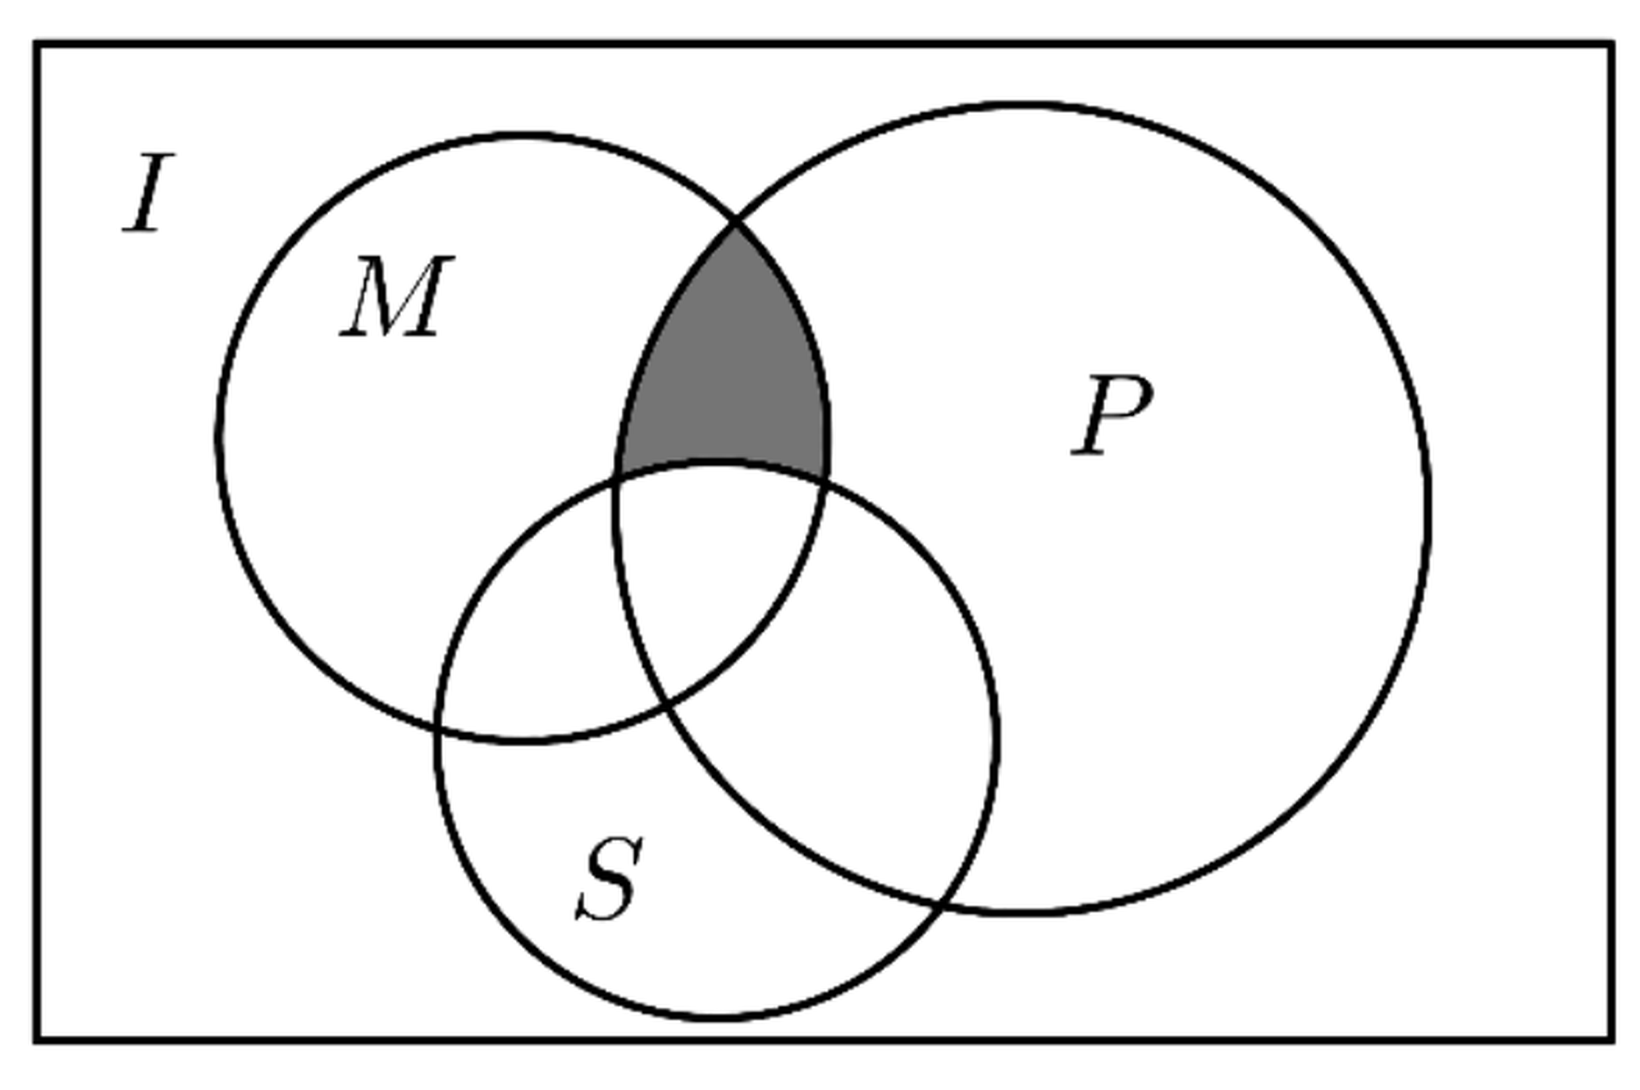
\includegraphics[width=0.42\textwidth]{figures/gao120_q15.png}
\end{center}

\keepwithprev
A. $(M\cap P)\cap S$\qquad\quad B. $(M\cap P)\cap\complement_{I}S$\qquad\quad C. $(M\cup P)\cap S$\qquad\quad D. $\complement_{I}(M\cap P)\cap S$

\ifanswer
\solbegin
\step{由已知中的 $Venn$ 图得阴影部分的元素属于 $M$，属于 $P$，但不属于 $S$，}
\step{所以阴影部分表示的集合为 $(M\cap P)\cap\complement_{I}S$，故选 $B$.}
\solend
\fi

\item 设集合 $P_1=\{x\mid x^2+ax+1>0\}$，$P_2=\{x\mid x^2+ax+2>0\}$，$Q_1=\{x\mid x^2+x+b>0\}$，$Q_2=\{x\mid x^2+2x+b>0\}$，其中 $a$、$b\in\R$，对于下列两个命题：①存在 $a$，$P_1$ 不是 $P_2$ 的子集；②存在 $b$ 使得 $Q_1$ 是 $Q_2$ 的子集. 下列说法正确的是\mbox{（\quad）}

\keepwithprev
A. ①是真命题，②是假命题\qquad\qquad B. ①是假命题，②是真命题

C. ①②都是真命题\qquad\qquad\qquad D. ①②都是假命题

\ifanswer
\solbegin
\step{对于集合 $P_1=\{x\mid x^2+ax+1>0\}$，$P_2=\{x\mid x^2+ax+2>0\}$，}
\step{得当 $m\in P_1$ 时，即 $m^2+am+1>0$，得 $m^2+am+2>0$，}
\step{即有 $m\in P_2$，得对任意 $a$，$P_1$ 是 $P_2$ 的子集，故①错误；}
\step{对于集合 $Q_1=\{x\mid x^2+x+b>0\}$，$Q_2=\{x\mid x^2+2x+b>0\}$，}
\step{当 $b=6$ 时，$Q_1=\{x\mid x^2+x+6>0\}=\R$，$Q_2=\{x\mid x^2+2x+6>0\}=\R$，}
\step{得 $Q_1$ 是 $Q_2$ 的子集，所以存在 $b$，使得 $Q_1$ 是 $Q_2$ 的子集，故②正确；}
\step{故选 $B$.}
\solend
\fi

\end{enumerate}

\bigsec{三、解答题}

\begin{enumerate}
\setcounter{enumi}{16}

\item (1) 已知 $x$、$y$ 都是实数，比较 $x^2+y^2$ 与 $4x-2y-5$ 的大小.

(2) 求解不等式组 $\begin{cases}x^2-4x+3\geqslant0\\\dfrac{x+3}{2x-1}\geqslant2\end{cases}$.

\ifanswer
\solbegin
\step{(1) $(x^2+y^2)-(4x-2y-5)=x^2-4x+y^2+2y+5=(x-2)^2+(y+1)^2\geqslant0$，}
\step{当 $x=2$，$y=-1$ 时，$x^2+y^2=4x-2y-5$.}
\step{当 $x\neq2$ 或 $y\neq-1$ 时，$x^2+y^2>4x-2y-5$.}
\step{(2) 由 $x^2-4x+3\geqslant0$ 得 $(x-1)(x-3)\geqslant0$，所以 $x\leqslant1$ 或 $x\geqslant3$；}
\step{由 $\dfrac{x+3}{2x-1}\geqslant2$，得 $\dfrac{x+3}{2x-1}-2=\dfrac{-3x+5}{2x-1}\geqslant0$，即 $\dfrac{3x-5}{2x-1}\leqslant0$，}
\step{所以 $\begin{cases}(3x-5)(2x-1)\leqslant0\\2x-1\neq0\end{cases}$，解得 $\dfrac12<x\leqslant\dfrac53$，}
\step{所以不等式组的解集是 $\left\{x\,\middle\vert\,\dfrac12<x\leqslant1\right\}$.}
\solend
\fi

\item 已知 $x_1$,$x_2$ 是一元二次方程 $4kx^2-4kx+k+1=0$ 的两个实数根.

(1) 是否存在实数 $k$，$(2x_1-x_2)(x_1-2x_2)=-\dfrac32$ 成立？若存在，求出 $k$ 的值；若不存在，请说明理由.

(2) 求使 $\dfrac{x_1}{x_2}+\dfrac{x_2}{x_1}-2$ 的值为整数的实数 $k$ 的整数值.

\ifanswer
\solbegin
\step{(1) 因为 $x_1$,$x_2$ 是一元二次方程 $4kx^2-4kx+k+1=0$ 的两个实数根，}
\step{所以 $\begin{cases}k\neq0\\16k^2-16k(k+1)\geqslant0\end{cases}$，所以 $k<0$，}
\step{由根与系数的关系得 $x_1+x_2=1$，$x_1x_2=\dfrac{k+1}{4k}$，}
\step{所以 $(2x_1-x_2)(x_1-2x_2)=2(x_1+x_2)^2-9x_1x_2=2-9\times\dfrac{k+1}{4k}=-\dfrac32$，}
\step{解得 $k=\dfrac95$，而 $k<0$，故不存在实数 $k$ 使得 $(2x_1-x_2)(x_1-2x_2)=-\dfrac32$ 成立.}
\step{(2) 由根与系数的关系得 $\dfrac{x_1}{x_2}+\dfrac{x_2}{x_1}-2=\dfrac{(x_1+x_2)^2}{x_1x_2}-4=-\dfrac4{k+1}$，}
\step{因为 $-\dfrac4{k+1}$ 的值为整数，而 $k$ 为整数，所以 $k+1$ 只能取 $\pm1$、$\pm2$、$\pm4$，}
\step{又 $k<0$，所以整数 $k$ 的值为 $-2$ 或 $-3$ 或 $-5$.}
\solend
\fi

\item 2026 年，某市低空经济蓬勃发展，一家物流企业开通“无人机即时配送”服务，并设立配送站. 经市场调研，该站每日配送单量 $y$（单位：单）与每单配送费 $x$（单位：元）满足关系式 $y=4800-200x$（其中 $4<x<24$）. 已知配送站每日的固定成本为 $19200$ 元，每完成一单配送，需支付电费、耗材费、设备保养费等可变成本，每单可变成本为 $4$ 元.

(1) 若要保证配送站每日利润 $W$（单位：元）不为负数，求每单配送费 $x$ 的取值范围；（每日利润 $=$ 每日配送总收入 $-$ 每日可变总成本 $-$ 每日固定成本）

(2) 为提升运力，该站购进一批新型无人机，购机费用为 $32$ 万元. 投入使用后，这批无人机使用 $t(t>0)$ 年的累计维保总费用为 $(2t^2+8t)$ 万元. 请问：这批无人机使用多少年后更新，可以使年平均总费用最低？请求出最低年平均总费用.（年平均总费用 $=$（购机费用 $+$ 维保总费用）$\div$ 使用年数）

\ifanswer
\solbegin
\step{(1) $W=xy-4y-19200=x(4800-200x)-4(4800-200x)-19200$}
\step{$=-200x^2+5600x-38400(4<x<24)$，}
\step{令 $W=-200x^2+5600x-38400\geqslant0$，即 $x^2-28x+192\leqslant0$，}
\step{解得 $12\leqslant x\leqslant16$，因此，要保证配送站每日利润 $W$ 不为负数，}
\step{每单配送费 $x$ 的取值范围为 $[12,16]$；}
\step{(2) 由题意，年平均总费用为 $N=\dfrac{2t^2+8t+32}{t}=2t+\dfrac{32}{t}+8$}
\step{$\geqslant2\sqrt{2t\cdot\dfrac{32}{t}}+8=16+8=24$，当且仅当 $2t=\dfrac{32}{t}$，即 $t=4$ 时取等号，}
\step{则这批无人机使用 $4$ 年后更新，可以使年平均总费用最低，}
\step{最低年平均总费用为 $24$ 万元.}
\solend
\fi

\item 已知 $A,B$，定义集合 $M_{(A,B)}=\{x\mid A<B\}$.

(1) 设 $A=\lvert x-4\rvert$,$B=2x$，求 $M_{(A,B)}$；

(2) 设 $A=ax^2+2ax-4$,$B=2x(x+2)$，当 $M_{(A,B)}=\R$ 时，求 $a$ 的取值范围；

(3) 设 $A=\lvert 2x-b\rvert$,$B=\dfrac{x+4b}{x-1}$,$C=2$，若 $M_{(A,C)}\cap M_{(B,C)}\neq\varnothing$，求 $b$ 的取值范围.

\ifanswer
\solbegin
\step{(1) 由定义，$x\in M_{(A,B)}$ 等价于 $\lvert x-4\rvert<2x$，}
\step{原不等式等价于 $-2x<x-4<2x$，即同时满足 $3x>4$ 与 $x>-4$，}
\step{解得 $x>\dfrac43$，所以 $M_{(A,B)}=\left(\dfrac43,+\infty\right)$.}
\step{(2) 由 $M_{(A,B)}=\R$，得 $ax^2+2ax-4<2x(x+2)$ 对任意 $x\in\R$ 恒成立，}
\step{得 $(a-2)(x+1)^2-a-2<0$.}
\step{当 $a>2$ 时，随着 $(x+1)^2$ 增大，左边可取正值，不符合题意；}
\step{当 $a=2$ 时，左边恒等于 $-4$，符合题意；}
\step{当 $a<2$ 时，左边在 $x=-1$ 处取得最大值 $-a-2$，}
\step{故恒成立的充要条件为 $-a-2<0$，即 $a>-2$；}
\step{综上，$a\in(-2,2]$.}
\step{(3) 由 $\lvert 2x-b\rvert<2$，得 $M_{(A,C)}=\left(\dfrac b2-1,\dfrac b2+1\right)$，记为 $I$.}
\step{由 $\dfrac{x+4b}{x-1}<2$，得 $\dfrac{x-(4b+2)}{x-1}>0$，其中 $x\neq1$.}
\step{①当 $b<-\dfrac14$ 时，$4b+2<1$，故 $M_{(B,C)}=(-\infty,4b+2)\cup(1,+\infty)$.}
\step{此时 $\dfrac b2+1<1$，所以 $I$ 与 $(1,+\infty)$ 没有公共元素.}
\step{两集合交集非空等价于 $\dfrac b2-1<4b+2$，解得 $b>-\dfrac67$.}
\step{因而本种情况得到 $-\dfrac67<b<-\dfrac14$.}
\step{②当 $b=-\dfrac14$ 时，$\dfrac{x+4b}{x-1}=1$，其中 $x\neq1$，故 $M_{(B,C)}=\{x\mid x\neq1\}$.}
\step{此时 $I=\left(-\dfrac98,\dfrac78\right)$，两集合交集非空.}
\step{③当 $b>-\dfrac14$ 时，$4b+2>1$，故 $M_{(B,C)}=(-\infty,1)\cup(4b+2,+\infty)$.}
\step{此时 $4b+2-\left(\dfrac b2+1\right)=\dfrac{7b}{2}+1>\dfrac18>0$，}
\step{所以 $I$ 与 $(4b+2,+\infty)$ 没有公共元素.}
\step{两集合交集非空等价于 $\dfrac b2-1<1$，解得 $b<4$.}
\step{因而本种情况得到 $-\dfrac14<b<4$.}
\step{综上，$b\in\left(-\dfrac67,4\right)$.}
\solend
\fi

\item 破晓同学阅读课外书籍时，发现笛卡尔积是代数和图论中一个很重要的课题. 对于非空数集 $A,B$，定义 $A\otimes B=\{(x,y)\mid x\in A$ 且 $y\in B\}$，将 $A\otimes B$ 称为“$A$ 与 $B$ 的笛卡尔积”.

(1) 若 $A=\{-1,0,1\}$,$B=\{-1,1\}$，求 $A\otimes B$ 和 $B\otimes A$；

(2) 试证明：“$A_1\otimes A_2=A_2\otimes A_1$”是“$A_1=A_2$”的充要条件；

(3) 若集合 $H$ 是有限集，将集合 $H$ 的元素个数记为 $\lvert H\rvert$. 已知 $\lvert A_1\otimes A_2\rvert=m^3(m\in\N^*)$，且存在实数 $a$ 满足 $\sqrt{\dfrac{\lvert A_1\otimes A_1\rvert+\lvert A_2\otimes A_2\rvert}{\lvert A_2\otimes A_1\rvert}}\geqslant a$ 对任意 $m\in\N^*$ 恒成立. 求 $a$ 的取值范围，并指明当 $a$ 取到最值时 $\lvert A_1\rvert$ 和 $\lvert A_2\rvert$ 满足的关系式及 $m$ 应满足的条件.

\ifanswer
\solbegin
\step{(1) 由题意得 $A\otimes B=\{(-1,-1),(-1,1),(0,-1),(0,1),(1,-1),(1,1)\}$，}
\step{$B\otimes A=\{(-1,-1),(-1,0),(-1,1),(1,-1),(1,0),(1,1)\}$；}
\step{(2) 若 $A_1=A_2$，设 $A_1=A_2=A$，}
\step{由定义得 $A_1\otimes A_2=\{(a,b)\mid a\in A$ 且 $b\in A\}=A_2\otimes A_1$，}
\step{所以“$A_1\otimes A_2=A_2\otimes A_1$”是“$A_1=A_2$”的必要条件；}
\step{若 $A_1\otimes A_2=A_2\otimes A_1$，对任意 $(a,b)\in A_1\otimes A_2$，均有 $(a,b)\in A_2\otimes A_1$，}
\step{即对任意 $a\in A_1,b\in A_2$，均有 $a\in A_2,b\in A_1$，}
\step{由任意性得 $A_1\subseteq A_2,A_2\subseteq A_1$，则 $A_1=A_2$，}
\step{所以“$A_1\otimes A_2=A_2\otimes A_1$”是“$A_1=A_2$”的充分条件；}
\step{综上所述，“$A_1\otimes A_2=A_2\otimes A_1$”是“$A_1=A_2$”的充要条件.}
\step{(3) 设 $\lvert A_1\rvert=c$,$\lvert A_2\rvert=d$,$c,d\in\N^*$，}
\step{则 $\lvert A_1\otimes A_2\rvert=\lvert A_2\otimes A_1\rvert=cd=m^3$,$\lvert A_1\otimes A_1\rvert=c^2$,$\lvert A_2\otimes A_2\rvert=d^2$，}
\step{得 $\sqrt{\dfrac{\lvert A_1\otimes A_1\rvert+\lvert A_2\otimes A_2\rvert}{\lvert A_2\otimes A_1\rvert}}=\sqrt{\dfrac{c^2+d^2}{cd}}=\sqrt{\dfrac cd+\dfrac dc}\geqslant\sqrt{2\sqrt{\dfrac cd\cdot\dfrac dc}}=\sqrt2$，}
\step{当且仅当 $\dfrac cd=\dfrac dc$，即 $c=d$ 时取等号，所以实数 $a$ 的取值范围是 $(-\infty,\sqrt2]$.}
\step{若 $a$ 取到最大值，则 $c=d$，即 $\lvert A_1\rvert=\lvert A_2\rvert$，得 $c^2=m^3$，}
\step{即 $c=\sqrt{m^3}=(\sqrt m)^3\in\N^*$，所以 $m=k^2,k\in\N^*$.}
\solend
\fi

\end{enumerate}

\end{document}
"
%
% 原始材料：微信公众号“魔都数学加油站”文章，作者破晓，2026-11-08 21:35 发布；
% 连载“27学年高一120”，原文标题“27学年高一120——2026-2027年上海市松江二中高一上10月月考”；
% 原文链接：https://mp.weixin.qq.com/s/hgDkaZX9M_IKhmr7CjQc1A。
% 正文为 10 张 PNG 页（第 8、10 页 2560×3620，其余 4762×6735），
% 题目下印有【解析】或【答案】，为讲评版。
% 题目、解析均据原图转录；卷面红色水印及公众号页脚未录入。
% 全卷 1 张插图：第 15 题的三集合 Venn 图（原卷印在题干右侧，本稿移至题干之后，
% 取原卷截图 2× LANCZOS 放大，见 figures/gao120_q15.png）。
%
% 卷首标题：原卷印作“2026-2027 年松江二中高一上 10 月月考”（公众号标题中的“上海市”
% 卷面标题行没有，本稿照卷面），年份区间按全稿惯例排 en dash；原卷未印副标题，本稿按题目内容
% 标为“集合与常用逻辑用语、不等式”（与 110／111／113／116／118 同）。
%
% 与原卷的排版差异：
%   ① 原文从第 3 题起，填空题编号为 3—12、选择题为 13—16、解答题为 17—21，本稿保留原题号；
%   ② 原卷每题下直接印【解析】／【答案】，本稿按全稿惯例置于答案版；第 3 题只印【答案】、
%      第 13、14 题把答案印在题干括号内且无【解析】，均另提 \ans{}；其余选择题答案在
%      解析末句“故选 …”，括号内留空；
%   ③ 原卷未印副标题，本稿按“知识模块”口径补出；
%   ④ 原卷填空横线按全稿惯例排为 \blankline[4.4em]；选择题括号排 \mbox{（\quad）}、
%      选项段前按惯例加 \keepwithprev；解答题不留作答区（原卷为讲评版，与 109—119 同）；
%   ⑤ 原卷数集排斜体 $R$、$N^*$，按全稿惯例改 \R、\N^*；绝对值排 \lvert…\rvert，
%      集合描述竖线排 \mid；补集记号照原卷排 \complement_I。
%
% 判别式字形：第 9 题解析作 $\triangle$（等边、扁），照录 \triangle。
%
% 子集符号：第 4 题题干与解析的 $A\subseteq B$、第 21 题 (2) 的 $A_1\subseteq A_2$ 印有下划线，
%   照录 \subseteq。
%
% 原卷存疑照录：第 12 题题干 $S=\{82,83,84,85,86,87,89\}$ 跳过 $88$ 只列 7 个数，
%   与其“8 种不同的值”自洽（不含 $88$），照录；第 19 题 (1) 的 $W$ 表达式
%   $x(4800-200x)-4(4800-200x)-19200$ 与最后结果 $[12,16]$ 一致。
%
% 行数核对：逐题数 \step 条数，合计 115 条（Q3：0；Q4：4；Q5：2；Q6：5；Q7：4；
% Q8：2；Q9：5；Q10：3；Q11：6；Q12：11；Q13：0；Q14：0；Q15：2；Q16：7；
% Q17：7；Q18：8；Q19：9；Q20：24；Q21：16），与原卷印刷行逐题相等
% （cases 块作一个印刷行计）。第 3 题只印【答案】、第 13、14 题括号内印答案且无解析，
% 均提 \ans{}，不计入 \step 账。
%
\documentclass[a4paper,11pt]{article}
\usepackage{common}

\begin{document}

\examtitlest[3]{2026--2027 年松江二中高一上 10 月月考}{集合与常用逻辑用语、不等式}

\bigsec{一、填空题}

\begin{enumerate}
\setcounter{enumi}{2}

\item 集合 $A=\{(x,y)\mid x+y=8\}$,$B=\{(x,y)\mid xy=12\}$，求 $A\cap B=$\blankline[4.4em].

\ifanswer
\ans{$\{(2,6),(6,2)\}$}
\fi

\item 设集合 $A=\{0,-a\}$,$B=\{1,a-2,2a-2\}$，若 $A\subseteq B$，则 $a=$\blankline[4.4em].

\ifanswer
\solbegin
\step{因为 $A\subseteq B$，}
\step{若 $a-2=0$，解得 $a=2$，此时 $A=\{0,-2\}$,$B=\{1,0,2\}$，不符合题意；}
\step{若 $2a-2=0$，解得 $a=1$，此时 $A=\{0,-1\}$,$B=\{1,-1,0\}$，符合题意；}
\step{综上所述，$a=1$.}
\solend
\fi

\item 设 $\alpha:0<x<a(a>0)$,$\beta:x<8-3a$，若 $\alpha$ 是 $\beta$ 的充分条件，则实数 $a$ 的取值范围是\blankline[4.4em].

\ifanswer
\solbegin
\step{由 $\alpha$ 是 $\beta$ 的充分条件得，$x\in(0,a)\Rightarrow x\in(-\infty,8-3a)$，}
\step{所以 $0<a\leqslant8-3a$，解得 $0<a\leqslant2$.}
\solend
\fi

\item 关于 $x$ 的不等式 $ax-b>0$ 的解集为 $(-\infty,1)$，则不等式 $\dfrac{x-2}{ax+b}<0$ 的解集为\blankline[4.4em].

\ifanswer
\solbegin
\step{因为关于 $x$ 的不等式 $ax-b>0$ 的解集为 $(-\infty,1)$，}
\step{所以 $a<0$ 且 $\dfrac ba=1$，则 $b=a$，}
\step{所以不等式 $\dfrac{x-2}{ax+b}<0$，即 $\dfrac{x-2}{ax+a}<0$，即 $\dfrac{x-2}{x+1}>0$，}
\step{等价于 $(x+1)(x-2)>0$，解得 $x>2$ 或 $x<-1$，}
\step{即解集为 $(-\infty,-1)\cup(2,+\infty)$.}
\solend
\fi

\item 若正实数 $x$、$y$ 满足 $2x+y+8xy=2$，则 $xy$ 的最大值为\blankline[4.4em].

\ifanswer
\solbegin
\step{因为正实数 $x$、$y$ 满足 $2x+y+8xy=2$，}
\step{所以 $2-8xy=2x+y\geqslant2\sqrt{2xy}$，}
\step{当且仅当 $y=2x$，即 $x=\dfrac14$，$y=\dfrac12$ 时取等号，解得 $0<xy\leqslant\dfrac18$，}
\step{故 $xy$ 的最大值为 $\dfrac18$.}
\solend
\fi

\item 已知 $1<a<3$，$-5<b<-2$，则 $\dfrac ab$ 的取值范围是\blankline[4.4em].

\ifanswer
\solbegin
\step{因为 $-5<b<-2$，所以 $2<-b<5$，$\dfrac15<-\dfrac1b<\dfrac12$，又 $1<a<3$，}
\step{得 $\dfrac15<-\dfrac ab<\dfrac32$，则 $-\dfrac32<\dfrac ab<-\dfrac15$，故 $\dfrac ab$ 的取值范围是 $\left(-\dfrac32,-\dfrac15\right)$.}
\solend
\fi

\item 若关于 $x$、$y$ 的方程组 $\begin{cases}y-kx-2=0\\y^2-4x-2y+1=0\end{cases}$ 的解集中只有一个元素，则实数 $k$ 的值为\blankline[4.4em].

\ifanswer
\solbegin
\step{由 $\begin{cases}y-kx-2=0\\y^2-4x-2y+1=0\end{cases}$ 消去 $y$ 整理得 $k^2x^2+(2k-4)x+1=0$.}
\step{当 $k\neq0$ 时，则 $\triangle=(2k-4)^2-4k^2=0$，解得 $k=1$，}
\step{此时方程组的解为 $\begin{cases}x=1\\y=3\end{cases}$，符合题意；}
\step{当 $k=0$ 时，解得 $x=\dfrac14$，此时方程组的解为 $\begin{cases}x=\dfrac14\\y=2\end{cases}$，符合题意；}
\step{综上，$k=0$ 或 $k=1$.}
\solend
\fi

\item 若集合 $A=\{0,1\}$，$B=\{x\mid x^2-mx-m>0,x\in\R\}$，且 $A\cap B=\{1\}$，则实数 $m$ 的取值范围为\blankline[4.4em].

\ifanswer
\solbegin
\step{因为集合 $A=\{0,1\}$，$B=\{x\mid x^2-mx-m>0,x\in\R\}$，且 $A\cap B=\{1\}$，}
\step{则 $1\in B$ 且 $0\notin B$，所以 $\begin{cases}1-m-m>0\\-m\leqslant0\end{cases}$，解得 $0\leqslant m<\dfrac12$，}
\step{所以实数 $m$ 的取值范围是 $\left[0,\dfrac12\right)$.}
\solend
\fi

\item 从集合 $U=\{a,b,c,d\}$ 的子集中选出两个不同的子集，需同时满足以下两个条件：(1) $a$、$b$ 都至少属于其中一个集合；(2) 对选出的两个子集，其中一个集合为另一个的子集，那么共有\blankline[4.4em]种不同的选法.

\ifanswer
\solbegin
\step{不妨设元素少的为 $A$，元素多的为 $B$，则 $B$ 必包含有 $a$、$b$；$A$ 为 $B$ 的真子集，}
\step{若 $B=\{a,b\}$，$A$ 为 $B$ 的真子集，共 $2^2-1=3$ 种，}
\step{若 $B=\{a,b,c\}$，$A$ 为 $B$ 的真子集，共 $2^3-1=7$ 种，}
\step{若 $B=\{a,b,d\}$，$A$ 为 $B$ 的真子集，共 $2^3-1=7$ 种，}
\step{若 $B=\{a,b,c,d\}$，$A$ 为 $B$ 的真子集，共 $2^4-1=15$ 种，}
\step{共有 $3+7+7+15=32$ 种.}
\solend
\fi

\item 已知 $a_1$、$a_2$、$\cdots$、$a_8$ 是 $8$ 个正整数，记 $S=\{a_{i_1}+a_{i_2}+\cdots+a_{i_7}\mid 1\leqslant i_1<i_2<\cdots<i_7\leqslant8\}$，其中 $i_1$、$i_2$、$\cdots$、$i_7\in\N^*$，若 $S=\{82,83,84,85,86,87,89\}$，则这 $8$ 个正整数中的最大数与最小数的积为\blankline[4.4em].

\ifanswer
\solbegin
\step{由题意得从 $8$ 个数中任取 $7$ 个数的和共有 $C_8^7=8$ 种不同的值，}
\step{但是 $82$，$83$，$84$，$85$，$86$，$87$，$89$ 只有 $7$ 个数，}
\step{得必有两种 $7$ 个数的和相等，设这个和为 $t(82\leqslant t\leqslant89)$，}
\step{令 $T=\sum\limits_{i=1}^{8}a_i$，那么，任取 $7$ 个数的和就等于 $T-a_i$，$i=1,2,\cdots,8$，}
\step{这 $8$ 个取值和的集合为 $S$，$S=\{T-a_1,T-a_2,\cdots,T-a_8\}$，}
\step{则 $\sum\limits_{i=1}^{8}(T-a_i)=8T-T=7T=82+83+84+85+86+87+89+t=596+t$.}
\step{因为 $T$ 为整数，所以 $596+t$ 是 $7$ 的倍数，}
\step{由 $596=7\times85+1$ 得 $1+t$ 是 $7$ 的倍数，}
\step{再因为 $82\leqslant t\leqslant89$，所以 $t=83$，得 $T=97$.}
\step{因此 $a_1$、$a_2$、$\cdots$、$a_8$ 中最大数为 $97-82=15$，最小数为 $97-89=8$，}
\step{因此，它们的积为 $120$.}
\solend
\fi

\end{enumerate}

\bigsec{二、选择题}

\begin{enumerate}
\setcounter{enumi}{12}

\item 已知 $a>b>0$，$c\in\R$，则下列不等式不一定成立的是\mbox{（\quad）}% 原卷把答案“$B$”印在题干括号内、无【解析】

\keepwithprev
A. $a-c>b-c$\qquad\quad B. $ac>bc$\qquad\quad C. $\dfrac1a<\dfrac1b$\qquad\quad D. $\dfrac{a+b}{2}>\sqrt{ab}$

\ifanswer
\ans{$B$}
\fi

\item 命题“对任意的 $x\in\R,x^3-x^2+1\leqslant0$”的否定是\mbox{（\quad）}% 原卷把答案“$C$”印在题干括号内、无【解析】

\keepwithprev
A. 不存在 $x\in\R,x^3-x^2+1\leqslant0$\qquad B. 存在 $x\in\R,x^3-x^2+1\leqslant0$

C. 存在 $x\in\R,x^3-x^2+1>0$\qquad\quad D. 对任意的 $x\in\R,x^3-x^2+1>0$

\ifanswer
\ans{$C$}
\fi

% 第 15 题是“题干 + 图 + 选项”约 6.5cm 的一整块，\keepwithprev 只挡得住“图—选项”，
% 挡不住夹在中间的图——实测断点落在题干之后（切页审计 A 类）。故照 高一30／高一26 成例
% 在题前先量一次页高，不够就把整块一起挪到次页。
\needvspace{7cm}
\item 如图，$I$ 是全集，$M$、$P$、$S$ 是 $I$ 的三个子集，则阴影部分所表示的集合是\mbox{（\quad）}

\begin{center}
% 图取原卷截图（第 4 页题干右侧）、2× LANCZOS 放大，本稿移至题干之后
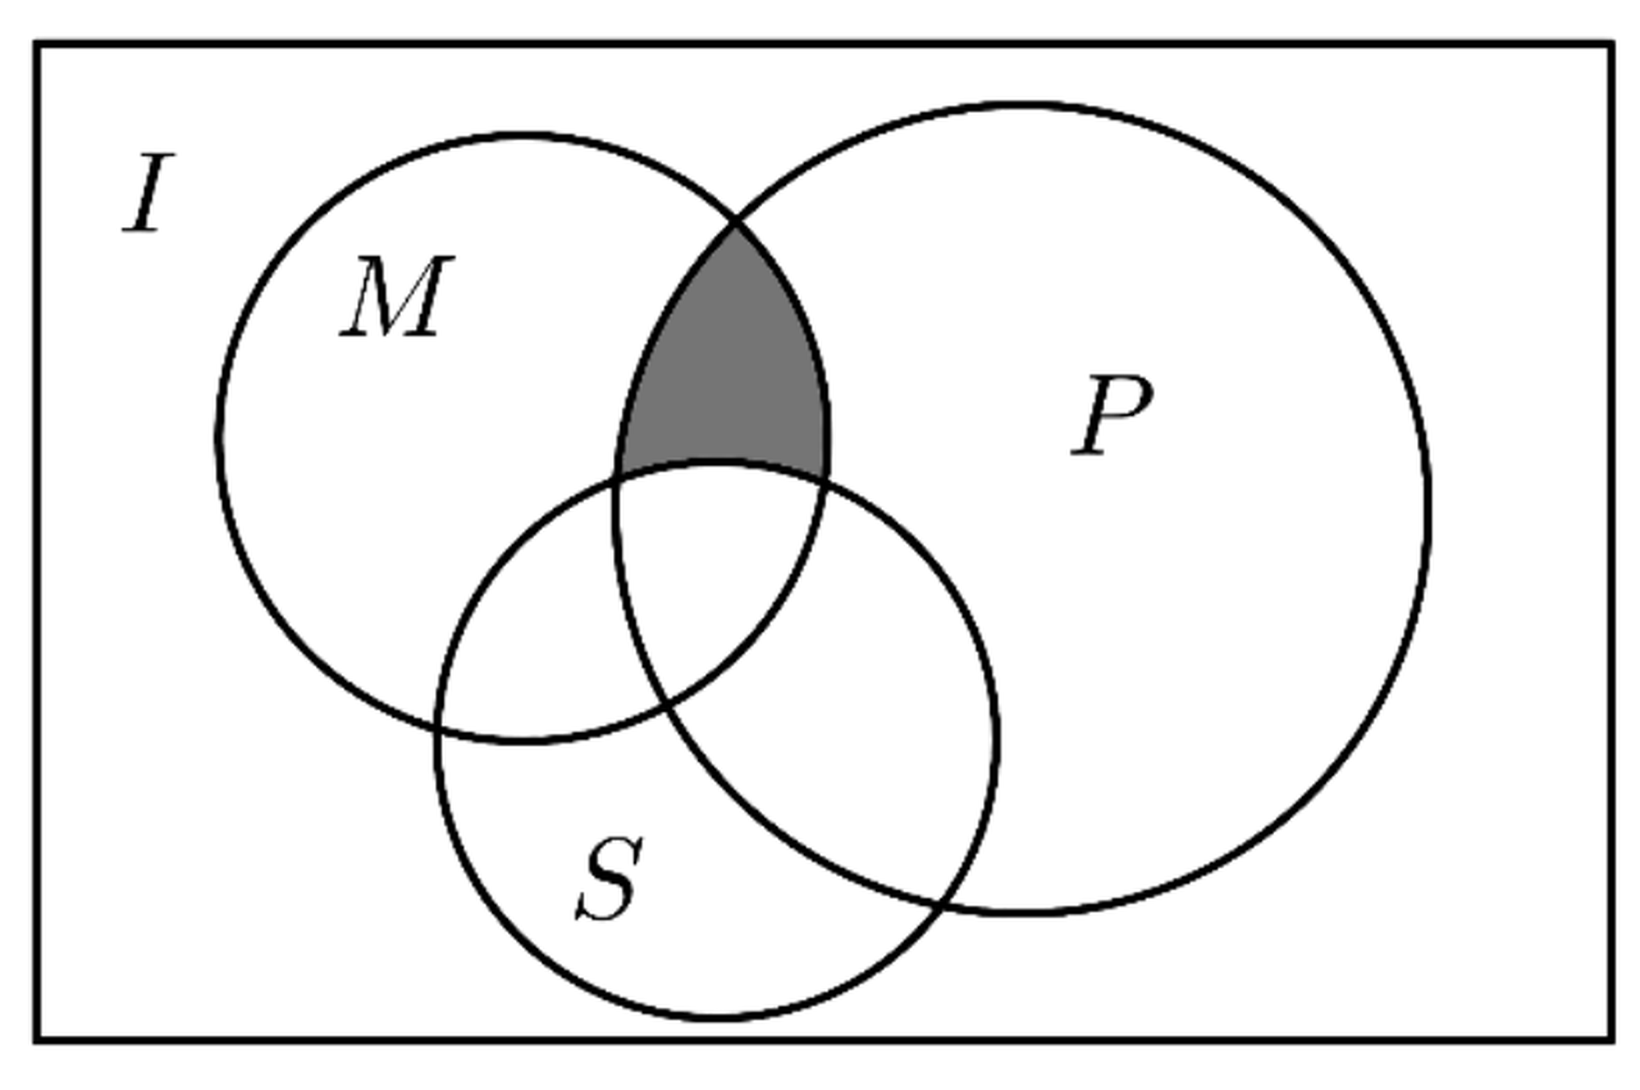
\includegraphics[width=0.42\textwidth]{figures/gao120_q15.png}
\end{center}

\keepwithprev
A. $(M\cap P)\cap S$\qquad\quad B. $(M\cap P)\cap\complement_{I}S$\qquad\quad C. $(M\cup P)\cap S$\qquad\quad D. $\complement_{I}(M\cap P)\cap S$

\ifanswer
\solbegin
\step{由已知中的 $Venn$ 图得阴影部分的元素属于 $M$，属于 $P$，但不属于 $S$，}
\step{所以阴影部分表示的集合为 $(M\cap P)\cap\complement_{I}S$，故选 $B$.}
\solend
\fi

\item 设集合 $P_1=\{x\mid x^2+ax+1>0\}$，$P_2=\{x\mid x^2+ax+2>0\}$，$Q_1=\{x\mid x^2+x+b>0\}$，$Q_2=\{x\mid x^2+2x+b>0\}$，其中 $a$、$b\in\R$，对于下列两个命题：①存在 $a$，$P_1$ 不是 $P_2$ 的子集；②存在 $b$ 使得 $Q_1$ 是 $Q_2$ 的子集. 下列说法正确的是\mbox{（\quad）}

\keepwithprev
A. ①是真命题，②是假命题\qquad\qquad B. ①是假命题，②是真命题

C. ①②都是真命题\qquad\qquad\qquad D. ①②都是假命题

\ifanswer
\solbegin
\step{对于集合 $P_1=\{x\mid x^2+ax+1>0\}$，$P_2=\{x\mid x^2+ax+2>0\}$，}
\step{得当 $m\in P_1$ 时，即 $m^2+am+1>0$，得 $m^2+am+2>0$，}
\step{即有 $m\in P_2$，得对任意 $a$，$P_1$ 是 $P_2$ 的子集，故①错误；}
\step{对于集合 $Q_1=\{x\mid x^2+x+b>0\}$，$Q_2=\{x\mid x^2+2x+b>0\}$，}
\step{当 $b=6$ 时，$Q_1=\{x\mid x^2+x+6>0\}=\R$，$Q_2=\{x\mid x^2+2x+6>0\}=\R$，}
\step{得 $Q_1$ 是 $Q_2$ 的子集，所以存在 $b$，使得 $Q_1$ 是 $Q_2$ 的子集，故②正确；}
\step{故选 $B$.}
\solend
\fi

\end{enumerate}

\bigsec{三、解答题}

\begin{enumerate}
\setcounter{enumi}{16}

\item (1) 已知 $x$、$y$ 都是实数，比较 $x^2+y^2$ 与 $4x-2y-5$ 的大小.

(2) 求解不等式组 $\begin{cases}x^2-4x+3\geqslant0\\\dfrac{x+3}{2x-1}\geqslant2\end{cases}$.

\ifanswer
\solbegin
\step{(1) $(x^2+y^2)-(4x-2y-5)=x^2-4x+y^2+2y+5=(x-2)^2+(y+1)^2\geqslant0$，}
\step{当 $x=2$，$y=-1$ 时，$x^2+y^2=4x-2y-5$.}
\step{当 $x\neq2$ 或 $y\neq-1$ 时，$x^2+y^2>4x-2y-5$.}
\step{(2) 由 $x^2-4x+3\geqslant0$ 得 $(x-1)(x-3)\geqslant0$，所以 $x\leqslant1$ 或 $x\geqslant3$；}
\step{由 $\dfrac{x+3}{2x-1}\geqslant2$，得 $\dfrac{x+3}{2x-1}-2=\dfrac{-3x+5}{2x-1}\geqslant0$，即 $\dfrac{3x-5}{2x-1}\leqslant0$，}
\step{所以 $\begin{cases}(3x-5)(2x-1)\leqslant0\\2x-1\neq0\end{cases}$，解得 $\dfrac12<x\leqslant\dfrac53$，}
\step{所以不等式组的解集是 $\left\{x\,\middle\vert\,\dfrac12<x\leqslant1\right\}$.}
\solend
\fi

\item 已知 $x_1$,$x_2$ 是一元二次方程 $4kx^2-4kx+k+1=0$ 的两个实数根.

(1) 是否存在实数 $k$，$(2x_1-x_2)(x_1-2x_2)=-\dfrac32$ 成立？若存在，求出 $k$ 的值；若不存在，请说明理由.

(2) 求使 $\dfrac{x_1}{x_2}+\dfrac{x_2}{x_1}-2$ 的值为整数的实数 $k$ 的整数值.

\ifanswer
\solbegin
\step{(1) 因为 $x_1$,$x_2$ 是一元二次方程 $4kx^2-4kx+k+1=0$ 的两个实数根，}
\step{所以 $\begin{cases}k\neq0\\16k^2-16k(k+1)\geqslant0\end{cases}$，所以 $k<0$，}
\step{由根与系数的关系得 $x_1+x_2=1$，$x_1x_2=\dfrac{k+1}{4k}$，}
\step{所以 $(2x_1-x_2)(x_1-2x_2)=2(x_1+x_2)^2-9x_1x_2=2-9\times\dfrac{k+1}{4k}=-\dfrac32$，}
\step{解得 $k=\dfrac95$，而 $k<0$，故不存在实数 $k$ 使得 $(2x_1-x_2)(x_1-2x_2)=-\dfrac32$ 成立.}
\step{(2) 由根与系数的关系得 $\dfrac{x_1}{x_2}+\dfrac{x_2}{x_1}-2=\dfrac{(x_1+x_2)^2}{x_1x_2}-4=-\dfrac4{k+1}$，}
\step{因为 $-\dfrac4{k+1}$ 的值为整数，而 $k$ 为整数，所以 $k+1$ 只能取 $\pm1$、$\pm2$、$\pm4$，}
\step{又 $k<0$，所以整数 $k$ 的值为 $-2$ 或 $-3$ 或 $-5$.}
\solend
\fi

\item 2026 年，某市低空经济蓬勃发展，一家物流企业开通“无人机即时配送”服务，并设立配送站. 经市场调研，该站每日配送单量 $y$（单位：单）与每单配送费 $x$（单位：元）满足关系式 $y=4800-200x$（其中 $4<x<24$）. 已知配送站每日的固定成本为 $19200$ 元，每完成一单配送，需支付电费、耗材费、设备保养费等可变成本，每单可变成本为 $4$ 元.

(1) 若要保证配送站每日利润 $W$（单位：元）不为负数，求每单配送费 $x$ 的取值范围；（每日利润 $=$ 每日配送总收入 $-$ 每日可变总成本 $-$ 每日固定成本）

(2) 为提升运力，该站购进一批新型无人机，购机费用为 $32$ 万元. 投入使用后，这批无人机使用 $t(t>0)$ 年的累计维保总费用为 $(2t^2+8t)$ 万元. 请问：这批无人机使用多少年后更新，可以使年平均总费用最低？请求出最低年平均总费用.（年平均总费用 $=$（购机费用 $+$ 维保总费用）$\div$ 使用年数）

\ifanswer
\solbegin
\step{(1) $W=xy-4y-19200=x(4800-200x)-4(4800-200x)-19200$}
\step{$=-200x^2+5600x-38400(4<x<24)$，}
\step{令 $W=-200x^2+5600x-38400\geqslant0$，即 $x^2-28x+192\leqslant0$，}
\step{解得 $12\leqslant x\leqslant16$，因此，要保证配送站每日利润 $W$ 不为负数，}
\step{每单配送费 $x$ 的取值范围为 $[12,16]$；}
\step{(2) 由题意，年平均总费用为 $N=\dfrac{2t^2+8t+32}{t}=2t+\dfrac{32}{t}+8$}
\step{$\geqslant2\sqrt{2t\cdot\dfrac{32}{t}}+8=16+8=24$，当且仅当 $2t=\dfrac{32}{t}$，即 $t=4$ 时取等号，}
\step{则这批无人机使用 $4$ 年后更新，可以使年平均总费用最低，}
\step{最低年平均总费用为 $24$ 万元.}
\solend
\fi

\item 已知 $A,B$，定义集合 $M_{(A,B)}=\{x\mid A<B\}$.

(1) 设 $A=\lvert x-4\rvert$,$B=2x$，求 $M_{(A,B)}$；

(2) 设 $A=ax^2+2ax-4$,$B=2x(x+2)$，当 $M_{(A,B)}=\R$ 时，求 $a$ 的取值范围；

(3) 设 $A=\lvert 2x-b\rvert$,$B=\dfrac{x+4b}{x-1}$,$C=2$，若 $M_{(A,C)}\cap M_{(B,C)}\neq\varnothing$，求 $b$ 的取值范围.

\ifanswer
\solbegin
\step{(1) 由定义，$x\in M_{(A,B)}$ 等价于 $\lvert x-4\rvert<2x$，}
\step{原不等式等价于 $-2x<x-4<2x$，即同时满足 $3x>4$ 与 $x>-4$，}
\step{解得 $x>\dfrac43$，所以 $M_{(A,B)}=\left(\dfrac43,+\infty\right)$.}
\step{(2) 由 $M_{(A,B)}=\R$，得 $ax^2+2ax-4<2x(x+2)$ 对任意 $x\in\R$ 恒成立，}
\step{得 $(a-2)(x+1)^2-a-2<0$.}
\step{当 $a>2$ 时，随着 $(x+1)^2$ 增大，左边可取正值，不符合题意；}
\step{当 $a=2$ 时，左边恒等于 $-4$，符合题意；}
\step{当 $a<2$ 时，左边在 $x=-1$ 处取得最大值 $-a-2$，}
\step{故恒成立的充要条件为 $-a-2<0$，即 $a>-2$；}
\step{综上，$a\in(-2,2]$.}
\step{(3) 由 $\lvert 2x-b\rvert<2$，得 $M_{(A,C)}=\left(\dfrac b2-1,\dfrac b2+1\right)$，记为 $I$.}
\step{由 $\dfrac{x+4b}{x-1}<2$，得 $\dfrac{x-(4b+2)}{x-1}>0$，其中 $x\neq1$.}
\step{①当 $b<-\dfrac14$ 时，$4b+2<1$，故 $M_{(B,C)}=(-\infty,4b+2)\cup(1,+\infty)$.}
\step{此时 $\dfrac b2+1<1$，所以 $I$ 与 $(1,+\infty)$ 没有公共元素.}
\step{两集合交集非空等价于 $\dfrac b2-1<4b+2$，解得 $b>-\dfrac67$.}
\step{因而本种情况得到 $-\dfrac67<b<-\dfrac14$.}
\step{②当 $b=-\dfrac14$ 时，$\dfrac{x+4b}{x-1}=1$，其中 $x\neq1$，故 $M_{(B,C)}=\{x\mid x\neq1\}$.}
\step{此时 $I=\left(-\dfrac98,\dfrac78\right)$，两集合交集非空.}
\step{③当 $b>-\dfrac14$ 时，$4b+2>1$，故 $M_{(B,C)}=(-\infty,1)\cup(4b+2,+\infty)$.}
\step{此时 $4b+2-\left(\dfrac b2+1\right)=\dfrac{7b}{2}+1>\dfrac18>0$，}
\step{所以 $I$ 与 $(4b+2,+\infty)$ 没有公共元素.}
\step{两集合交集非空等价于 $\dfrac b2-1<1$，解得 $b<4$.}
\step{因而本种情况得到 $-\dfrac14<b<4$.}
\step{综上，$b\in\left(-\dfrac67,4\right)$.}
\solend
\fi

\item 破晓同学阅读课外书籍时，发现笛卡尔积是代数和图论中一个很重要的课题. 对于非空数集 $A,B$，定义 $A\otimes B=\{(x,y)\mid x\in A$ 且 $y\in B\}$，将 $A\otimes B$ 称为“$A$ 与 $B$ 的笛卡尔积”.

(1) 若 $A=\{-1,0,1\}$,$B=\{-1,1\}$，求 $A\otimes B$ 和 $B\otimes A$；

(2) 试证明：“$A_1\otimes A_2=A_2\otimes A_1$”是“$A_1=A_2$”的充要条件；

(3) 若集合 $H$ 是有限集，将集合 $H$ 的元素个数记为 $\lvert H\rvert$. 已知 $\lvert A_1\otimes A_2\rvert=m^3(m\in\N^*)$，且存在实数 $a$ 满足 $\sqrt{\dfrac{\lvert A_1\otimes A_1\rvert+\lvert A_2\otimes A_2\rvert}{\lvert A_2\otimes A_1\rvert}}\geqslant a$ 对任意 $m\in\N^*$ 恒成立. 求 $a$ 的取值范围，并指明当 $a$ 取到最值时 $\lvert A_1\rvert$ 和 $\lvert A_2\rvert$ 满足的关系式及 $m$ 应满足的条件.

\ifanswer
\solbegin
\step{(1) 由题意得 $A\otimes B=\{(-1,-1),(-1,1),(0,-1),(0,1),(1,-1),(1,1)\}$，}
\step{$B\otimes A=\{(-1,-1),(-1,0),(-1,1),(1,-1),(1,0),(1,1)\}$；}
\step{(2) 若 $A_1=A_2$，设 $A_1=A_2=A$，}
\step{由定义得 $A_1\otimes A_2=\{(a,b)\mid a\in A$ 且 $b\in A\}=A_2\otimes A_1$，}
\step{所以“$A_1\otimes A_2=A_2\otimes A_1$”是“$A_1=A_2$”的必要条件；}
\step{若 $A_1\otimes A_2=A_2\otimes A_1$，对任意 $(a,b)\in A_1\otimes A_2$，均有 $(a,b)\in A_2\otimes A_1$，}
\step{即对任意 $a\in A_1,b\in A_2$，均有 $a\in A_2,b\in A_1$，}
\step{由任意性得 $A_1\subseteq A_2,A_2\subseteq A_1$，则 $A_1=A_2$，}
\step{所以“$A_1\otimes A_2=A_2\otimes A_1$”是“$A_1=A_2$”的充分条件；}
\step{综上所述，“$A_1\otimes A_2=A_2\otimes A_1$”是“$A_1=A_2$”的充要条件.}
\step{(3) 设 $\lvert A_1\rvert=c$,$\lvert A_2\rvert=d$,$c,d\in\N^*$，}
\step{则 $\lvert A_1\otimes A_2\rvert=\lvert A_2\otimes A_1\rvert=cd=m^3$,$\lvert A_1\otimes A_1\rvert=c^2$,$\lvert A_2\otimes A_2\rvert=d^2$，}
\step{得 $\sqrt{\dfrac{\lvert A_1\otimes A_1\rvert+\lvert A_2\otimes A_2\rvert}{\lvert A_2\otimes A_1\rvert}}=\sqrt{\dfrac{c^2+d^2}{cd}}=\sqrt{\dfrac cd+\dfrac dc}\geqslant\sqrt{2\sqrt{\dfrac cd\cdot\dfrac dc}}=\sqrt2$，}
\step{当且仅当 $\dfrac cd=\dfrac dc$，即 $c=d$ 时取等号，所以实数 $a$ 的取值范围是 $(-\infty,\sqrt2]$.}
\step{若 $a$ 取到最大值，则 $c=d$，即 $\lvert A_1\rvert=\lvert A_2\rvert$，得 $c^2=m^3$，}
\step{即 $c=\sqrt{m^3}=(\sqrt m)^3\in\N^*$，所以 $m=k^2,k\in\N^*$.}
\solend
\fi

\end{enumerate}

\end{document}
"
% 紧凑版：xelatex "\def\iscompact{1}% 高一120_松江二中_10月月考.tex
%   —— 高一上数学“2026-2027 年松江二中高一上 10 月月考”（试卷版/答案版）
% 试卷版：xelatex 高一120_松江二中_10月月考.tex
% 答案版：xelatex "\def\isanswer{1}% 高一120_松江二中_10月月考.tex
%   —— 高一上数学“2026-2027 年松江二中高一上 10 月月考”（试卷版/答案版）
% 试卷版：xelatex 高一120_松江二中_10月月考.tex
% 答案版：xelatex "\def\isanswer{1}\input{高一120_松江二中_10月月考.tex}"
% 紧凑版：xelatex "\def\iscompact{1}\input{高一120_松江二中_10月月考.tex}"
%
% 原始材料：微信公众号“魔都数学加油站”文章，作者破晓，2026-11-08 21:35 发布；
% 连载“27学年高一120”，原文标题“27学年高一120——2026-2027年上海市松江二中高一上10月月考”；
% 原文链接：https://mp.weixin.qq.com/s/hgDkaZX9M_IKhmr7CjQc1A。
% 正文为 10 张 PNG 页（第 8、10 页 2560×3620，其余 4762×6735），
% 题目下印有【解析】或【答案】，为讲评版。
% 题目、解析均据原图转录；卷面红色水印及公众号页脚未录入。
% 全卷 1 张插图：第 15 题的三集合 Venn 图（原卷印在题干右侧，本稿移至题干之后，
% 取原卷截图 2× LANCZOS 放大，见 figures/gao120_q15.png）。
%
% 卷首标题：原卷印作“2026-2027 年松江二中高一上 10 月月考”（公众号标题中的“上海市”
% 卷面标题行没有，本稿照卷面），年份区间按全稿惯例排 en dash；原卷未印副标题，本稿按题目内容
% 标为“集合与常用逻辑用语、不等式”（与 110／111／113／116／118 同）。
%
% 与原卷的排版差异：
%   ① 原文从第 3 题起，填空题编号为 3—12、选择题为 13—16、解答题为 17—21，本稿保留原题号；
%   ② 原卷每题下直接印【解析】／【答案】，本稿按全稿惯例置于答案版；第 3 题只印【答案】、
%      第 13、14 题把答案印在题干括号内且无【解析】，均另提 \ans{}；其余选择题答案在
%      解析末句“故选 …”，括号内留空；
%   ③ 原卷未印副标题，本稿按“知识模块”口径补出；
%   ④ 原卷填空横线按全稿惯例排为 \blankline[4.4em]；选择题括号排 \mbox{（\quad）}、
%      选项段前按惯例加 \keepwithprev；解答题不留作答区（原卷为讲评版，与 109—119 同）；
%   ⑤ 原卷数集排斜体 $R$、$N^*$，按全稿惯例改 \R、\N^*；绝对值排 \lvert…\rvert，
%      集合描述竖线排 \mid；补集记号照原卷排 \complement_I。
%
% 判别式字形：第 9 题解析作 $\triangle$（等边、扁），照录 \triangle。
%
% 子集符号：第 4 题题干与解析的 $A\subseteq B$、第 21 题 (2) 的 $A_1\subseteq A_2$ 印有下划线，
%   照录 \subseteq。
%
% 原卷存疑照录：第 12 题题干 $S=\{82,83,84,85,86,87,89\}$ 跳过 $88$ 只列 7 个数，
%   与其“8 种不同的值”自洽（不含 $88$），照录；第 19 题 (1) 的 $W$ 表达式
%   $x(4800-200x)-4(4800-200x)-19200$ 与最后结果 $[12,16]$ 一致。
%
% 行数核对：逐题数 \step 条数，合计 115 条（Q3：0；Q4：4；Q5：2；Q6：5；Q7：4；
% Q8：2；Q9：5；Q10：3；Q11：6；Q12：11；Q13：0；Q14：0；Q15：2；Q16：7；
% Q17：7；Q18：8；Q19：9；Q20：24；Q21：16），与原卷印刷行逐题相等
% （cases 块作一个印刷行计）。第 3 题只印【答案】、第 13、14 题括号内印答案且无解析，
% 均提 \ans{}，不计入 \step 账。
%
\documentclass[a4paper,11pt]{article}
\usepackage{common}

\begin{document}

\examtitlest[3]{2026--2027 年松江二中高一上 10 月月考}{集合与常用逻辑用语、不等式}

\bigsec{一、填空题}

\begin{enumerate}
\setcounter{enumi}{2}

\item 集合 $A=\{(x,y)\mid x+y=8\}$,$B=\{(x,y)\mid xy=12\}$，求 $A\cap B=$\blankline[4.4em].

\ifanswer
\ans{$\{(2,6),(6,2)\}$}
\fi

\item 设集合 $A=\{0,-a\}$,$B=\{1,a-2,2a-2\}$，若 $A\subseteq B$，则 $a=$\blankline[4.4em].

\ifanswer
\solbegin
\step{因为 $A\subseteq B$，}
\step{若 $a-2=0$，解得 $a=2$，此时 $A=\{0,-2\}$,$B=\{1,0,2\}$，不符合题意；}
\step{若 $2a-2=0$，解得 $a=1$，此时 $A=\{0,-1\}$,$B=\{1,-1,0\}$，符合题意；}
\step{综上所述，$a=1$.}
\solend
\fi

\item 设 $\alpha:0<x<a(a>0)$,$\beta:x<8-3a$，若 $\alpha$ 是 $\beta$ 的充分条件，则实数 $a$ 的取值范围是\blankline[4.4em].

\ifanswer
\solbegin
\step{由 $\alpha$ 是 $\beta$ 的充分条件得，$x\in(0,a)\Rightarrow x\in(-\infty,8-3a)$，}
\step{所以 $0<a\leqslant8-3a$，解得 $0<a\leqslant2$.}
\solend
\fi

\item 关于 $x$ 的不等式 $ax-b>0$ 的解集为 $(-\infty,1)$，则不等式 $\dfrac{x-2}{ax+b}<0$ 的解集为\blankline[4.4em].

\ifanswer
\solbegin
\step{因为关于 $x$ 的不等式 $ax-b>0$ 的解集为 $(-\infty,1)$，}
\step{所以 $a<0$ 且 $\dfrac ba=1$，则 $b=a$，}
\step{所以不等式 $\dfrac{x-2}{ax+b}<0$，即 $\dfrac{x-2}{ax+a}<0$，即 $\dfrac{x-2}{x+1}>0$，}
\step{等价于 $(x+1)(x-2)>0$，解得 $x>2$ 或 $x<-1$，}
\step{即解集为 $(-\infty,-1)\cup(2,+\infty)$.}
\solend
\fi

\item 若正实数 $x$、$y$ 满足 $2x+y+8xy=2$，则 $xy$ 的最大值为\blankline[4.4em].

\ifanswer
\solbegin
\step{因为正实数 $x$、$y$ 满足 $2x+y+8xy=2$，}
\step{所以 $2-8xy=2x+y\geqslant2\sqrt{2xy}$，}
\step{当且仅当 $y=2x$，即 $x=\dfrac14$，$y=\dfrac12$ 时取等号，解得 $0<xy\leqslant\dfrac18$，}
\step{故 $xy$ 的最大值为 $\dfrac18$.}
\solend
\fi

\item 已知 $1<a<3$，$-5<b<-2$，则 $\dfrac ab$ 的取值范围是\blankline[4.4em].

\ifanswer
\solbegin
\step{因为 $-5<b<-2$，所以 $2<-b<5$，$\dfrac15<-\dfrac1b<\dfrac12$，又 $1<a<3$，}
\step{得 $\dfrac15<-\dfrac ab<\dfrac32$，则 $-\dfrac32<\dfrac ab<-\dfrac15$，故 $\dfrac ab$ 的取值范围是 $\left(-\dfrac32,-\dfrac15\right)$.}
\solend
\fi

\item 若关于 $x$、$y$ 的方程组 $\begin{cases}y-kx-2=0\\y^2-4x-2y+1=0\end{cases}$ 的解集中只有一个元素，则实数 $k$ 的值为\blankline[4.4em].

\ifanswer
\solbegin
\step{由 $\begin{cases}y-kx-2=0\\y^2-4x-2y+1=0\end{cases}$ 消去 $y$ 整理得 $k^2x^2+(2k-4)x+1=0$.}
\step{当 $k\neq0$ 时，则 $\triangle=(2k-4)^2-4k^2=0$，解得 $k=1$，}
\step{此时方程组的解为 $\begin{cases}x=1\\y=3\end{cases}$，符合题意；}
\step{当 $k=0$ 时，解得 $x=\dfrac14$，此时方程组的解为 $\begin{cases}x=\dfrac14\\y=2\end{cases}$，符合题意；}
\step{综上，$k=0$ 或 $k=1$.}
\solend
\fi

\item 若集合 $A=\{0,1\}$，$B=\{x\mid x^2-mx-m>0,x\in\R\}$，且 $A\cap B=\{1\}$，则实数 $m$ 的取值范围为\blankline[4.4em].

\ifanswer
\solbegin
\step{因为集合 $A=\{0,1\}$，$B=\{x\mid x^2-mx-m>0,x\in\R\}$，且 $A\cap B=\{1\}$，}
\step{则 $1\in B$ 且 $0\notin B$，所以 $\begin{cases}1-m-m>0\\-m\leqslant0\end{cases}$，解得 $0\leqslant m<\dfrac12$，}
\step{所以实数 $m$ 的取值范围是 $\left[0,\dfrac12\right)$.}
\solend
\fi

\item 从集合 $U=\{a,b,c,d\}$ 的子集中选出两个不同的子集，需同时满足以下两个条件：(1) $a$、$b$ 都至少属于其中一个集合；(2) 对选出的两个子集，其中一个集合为另一个的子集，那么共有\blankline[4.4em]种不同的选法.

\ifanswer
\solbegin
\step{不妨设元素少的为 $A$，元素多的为 $B$，则 $B$ 必包含有 $a$、$b$；$A$ 为 $B$ 的真子集，}
\step{若 $B=\{a,b\}$，$A$ 为 $B$ 的真子集，共 $2^2-1=3$ 种，}
\step{若 $B=\{a,b,c\}$，$A$ 为 $B$ 的真子集，共 $2^3-1=7$ 种，}
\step{若 $B=\{a,b,d\}$，$A$ 为 $B$ 的真子集，共 $2^3-1=7$ 种，}
\step{若 $B=\{a,b,c,d\}$，$A$ 为 $B$ 的真子集，共 $2^4-1=15$ 种，}
\step{共有 $3+7+7+15=32$ 种.}
\solend
\fi

\item 已知 $a_1$、$a_2$、$\cdots$、$a_8$ 是 $8$ 个正整数，记 $S=\{a_{i_1}+a_{i_2}+\cdots+a_{i_7}\mid 1\leqslant i_1<i_2<\cdots<i_7\leqslant8\}$，其中 $i_1$、$i_2$、$\cdots$、$i_7\in\N^*$，若 $S=\{82,83,84,85,86,87,89\}$，则这 $8$ 个正整数中的最大数与最小数的积为\blankline[4.4em].

\ifanswer
\solbegin
\step{由题意得从 $8$ 个数中任取 $7$ 个数的和共有 $C_8^7=8$ 种不同的值，}
\step{但是 $82$，$83$，$84$，$85$，$86$，$87$，$89$ 只有 $7$ 个数，}
\step{得必有两种 $7$ 个数的和相等，设这个和为 $t(82\leqslant t\leqslant89)$，}
\step{令 $T=\sum\limits_{i=1}^{8}a_i$，那么，任取 $7$ 个数的和就等于 $T-a_i$，$i=1,2,\cdots,8$，}
\step{这 $8$ 个取值和的集合为 $S$，$S=\{T-a_1,T-a_2,\cdots,T-a_8\}$，}
\step{则 $\sum\limits_{i=1}^{8}(T-a_i)=8T-T=7T=82+83+84+85+86+87+89+t=596+t$.}
\step{因为 $T$ 为整数，所以 $596+t$ 是 $7$ 的倍数，}
\step{由 $596=7\times85+1$ 得 $1+t$ 是 $7$ 的倍数，}
\step{再因为 $82\leqslant t\leqslant89$，所以 $t=83$，得 $T=97$.}
\step{因此 $a_1$、$a_2$、$\cdots$、$a_8$ 中最大数为 $97-82=15$，最小数为 $97-89=8$，}
\step{因此，它们的积为 $120$.}
\solend
\fi

\end{enumerate}

\bigsec{二、选择题}

\begin{enumerate}
\setcounter{enumi}{12}

\item 已知 $a>b>0$，$c\in\R$，则下列不等式不一定成立的是\mbox{（\quad）}% 原卷把答案“$B$”印在题干括号内、无【解析】

\keepwithprev
A. $a-c>b-c$\qquad\quad B. $ac>bc$\qquad\quad C. $\dfrac1a<\dfrac1b$\qquad\quad D. $\dfrac{a+b}{2}>\sqrt{ab}$

\ifanswer
\ans{$B$}
\fi

\item 命题“对任意的 $x\in\R,x^3-x^2+1\leqslant0$”的否定是\mbox{（\quad）}% 原卷把答案“$C$”印在题干括号内、无【解析】

\keepwithprev
A. 不存在 $x\in\R,x^3-x^2+1\leqslant0$\qquad B. 存在 $x\in\R,x^3-x^2+1\leqslant0$

C. 存在 $x\in\R,x^3-x^2+1>0$\qquad\quad D. 对任意的 $x\in\R,x^3-x^2+1>0$

\ifanswer
\ans{$C$}
\fi

% 第 15 题是“题干 + 图 + 选项”约 6.5cm 的一整块，\keepwithprev 只挡得住“图—选项”，
% 挡不住夹在中间的图——实测断点落在题干之后（切页审计 A 类）。故照 高一30／高一26 成例
% 在题前先量一次页高，不够就把整块一起挪到次页。
\needvspace{7cm}
\item 如图，$I$ 是全集，$M$、$P$、$S$ 是 $I$ 的三个子集，则阴影部分所表示的集合是\mbox{（\quad）}

\begin{center}
% 图取原卷截图（第 4 页题干右侧）、2× LANCZOS 放大，本稿移至题干之后
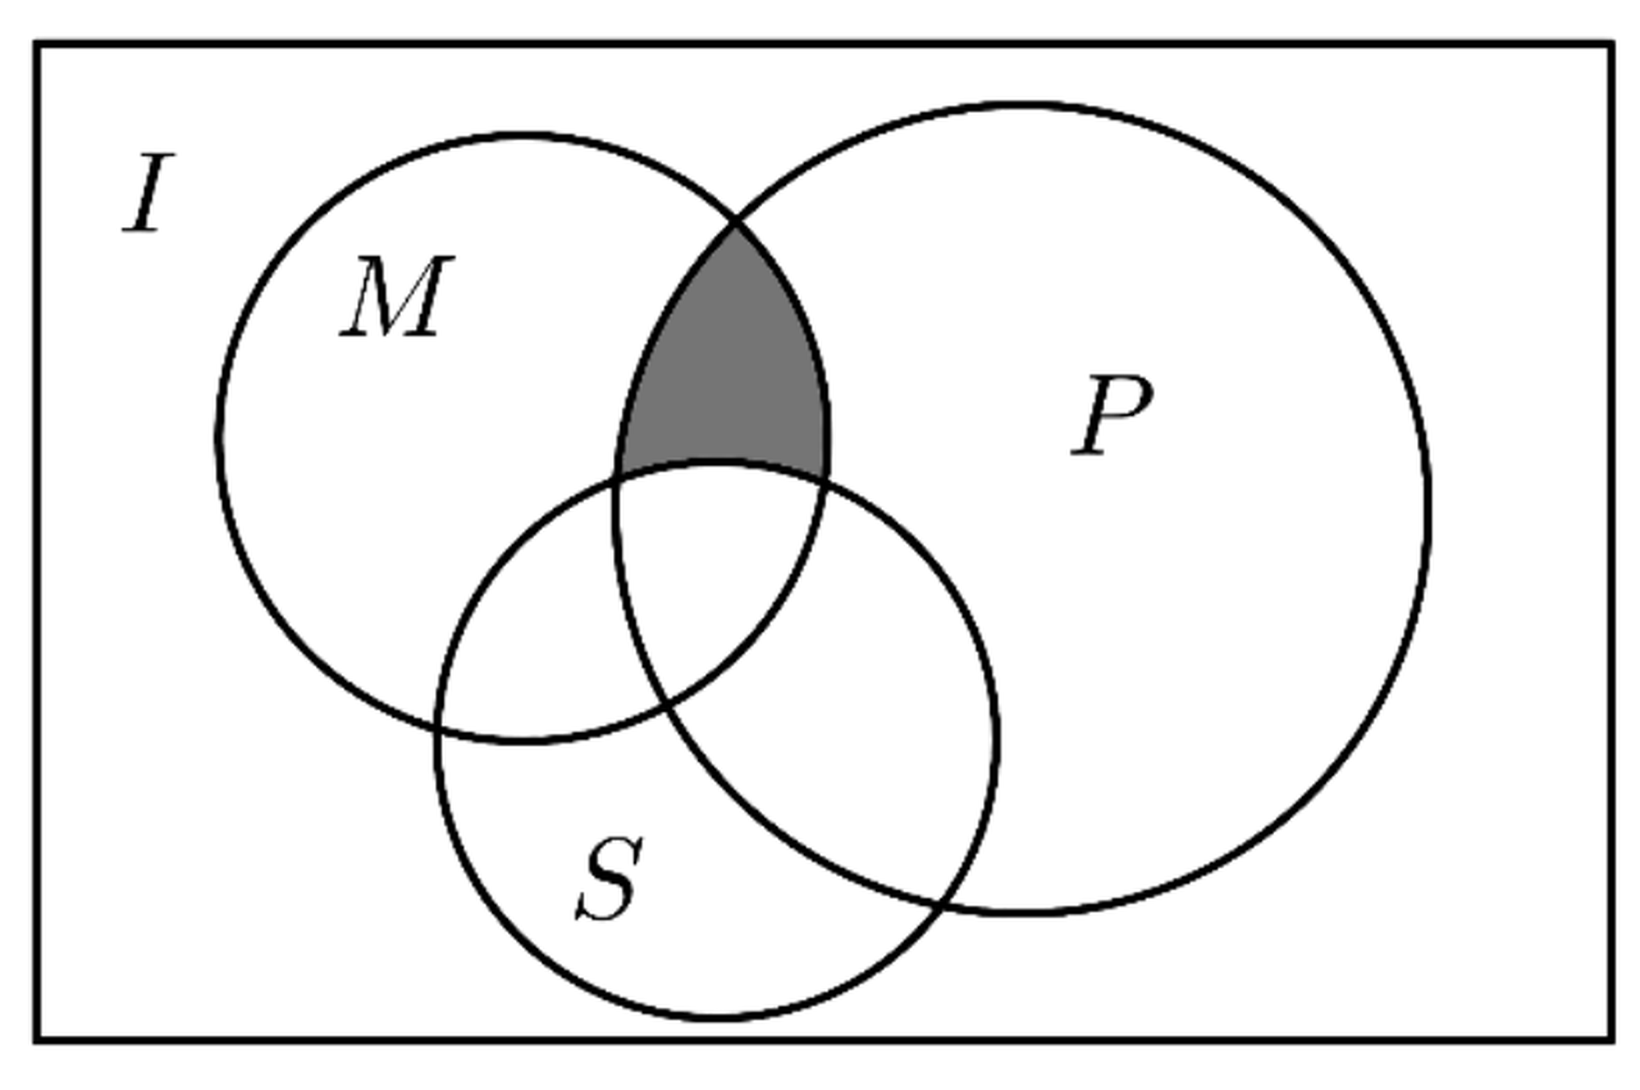
\includegraphics[width=0.42\textwidth]{figures/gao120_q15.png}
\end{center}

\keepwithprev
A. $(M\cap P)\cap S$\qquad\quad B. $(M\cap P)\cap\complement_{I}S$\qquad\quad C. $(M\cup P)\cap S$\qquad\quad D. $\complement_{I}(M\cap P)\cap S$

\ifanswer
\solbegin
\step{由已知中的 $Venn$ 图得阴影部分的元素属于 $M$，属于 $P$，但不属于 $S$，}
\step{所以阴影部分表示的集合为 $(M\cap P)\cap\complement_{I}S$，故选 $B$.}
\solend
\fi

\item 设集合 $P_1=\{x\mid x^2+ax+1>0\}$，$P_2=\{x\mid x^2+ax+2>0\}$，$Q_1=\{x\mid x^2+x+b>0\}$，$Q_2=\{x\mid x^2+2x+b>0\}$，其中 $a$、$b\in\R$，对于下列两个命题：①存在 $a$，$P_1$ 不是 $P_2$ 的子集；②存在 $b$ 使得 $Q_1$ 是 $Q_2$ 的子集. 下列说法正确的是\mbox{（\quad）}

\keepwithprev
A. ①是真命题，②是假命题\qquad\qquad B. ①是假命题，②是真命题

C. ①②都是真命题\qquad\qquad\qquad D. ①②都是假命题

\ifanswer
\solbegin
\step{对于集合 $P_1=\{x\mid x^2+ax+1>0\}$，$P_2=\{x\mid x^2+ax+2>0\}$，}
\step{得当 $m\in P_1$ 时，即 $m^2+am+1>0$，得 $m^2+am+2>0$，}
\step{即有 $m\in P_2$，得对任意 $a$，$P_1$ 是 $P_2$ 的子集，故①错误；}
\step{对于集合 $Q_1=\{x\mid x^2+x+b>0\}$，$Q_2=\{x\mid x^2+2x+b>0\}$，}
\step{当 $b=6$ 时，$Q_1=\{x\mid x^2+x+6>0\}=\R$，$Q_2=\{x\mid x^2+2x+6>0\}=\R$，}
\step{得 $Q_1$ 是 $Q_2$ 的子集，所以存在 $b$，使得 $Q_1$ 是 $Q_2$ 的子集，故②正确；}
\step{故选 $B$.}
\solend
\fi

\end{enumerate}

\bigsec{三、解答题}

\begin{enumerate}
\setcounter{enumi}{16}

\item (1) 已知 $x$、$y$ 都是实数，比较 $x^2+y^2$ 与 $4x-2y-5$ 的大小.

(2) 求解不等式组 $\begin{cases}x^2-4x+3\geqslant0\\\dfrac{x+3}{2x-1}\geqslant2\end{cases}$.

\ifanswer
\solbegin
\step{(1) $(x^2+y^2)-(4x-2y-5)=x^2-4x+y^2+2y+5=(x-2)^2+(y+1)^2\geqslant0$，}
\step{当 $x=2$，$y=-1$ 时，$x^2+y^2=4x-2y-5$.}
\step{当 $x\neq2$ 或 $y\neq-1$ 时，$x^2+y^2>4x-2y-5$.}
\step{(2) 由 $x^2-4x+3\geqslant0$ 得 $(x-1)(x-3)\geqslant0$，所以 $x\leqslant1$ 或 $x\geqslant3$；}
\step{由 $\dfrac{x+3}{2x-1}\geqslant2$，得 $\dfrac{x+3}{2x-1}-2=\dfrac{-3x+5}{2x-1}\geqslant0$，即 $\dfrac{3x-5}{2x-1}\leqslant0$，}
\step{所以 $\begin{cases}(3x-5)(2x-1)\leqslant0\\2x-1\neq0\end{cases}$，解得 $\dfrac12<x\leqslant\dfrac53$，}
\step{所以不等式组的解集是 $\left\{x\,\middle\vert\,\dfrac12<x\leqslant1\right\}$.}
\solend
\fi

\item 已知 $x_1$,$x_2$ 是一元二次方程 $4kx^2-4kx+k+1=0$ 的两个实数根.

(1) 是否存在实数 $k$，$(2x_1-x_2)(x_1-2x_2)=-\dfrac32$ 成立？若存在，求出 $k$ 的值；若不存在，请说明理由.

(2) 求使 $\dfrac{x_1}{x_2}+\dfrac{x_2}{x_1}-2$ 的值为整数的实数 $k$ 的整数值.

\ifanswer
\solbegin
\step{(1) 因为 $x_1$,$x_2$ 是一元二次方程 $4kx^2-4kx+k+1=0$ 的两个实数根，}
\step{所以 $\begin{cases}k\neq0\\16k^2-16k(k+1)\geqslant0\end{cases}$，所以 $k<0$，}
\step{由根与系数的关系得 $x_1+x_2=1$，$x_1x_2=\dfrac{k+1}{4k}$，}
\step{所以 $(2x_1-x_2)(x_1-2x_2)=2(x_1+x_2)^2-9x_1x_2=2-9\times\dfrac{k+1}{4k}=-\dfrac32$，}
\step{解得 $k=\dfrac95$，而 $k<0$，故不存在实数 $k$ 使得 $(2x_1-x_2)(x_1-2x_2)=-\dfrac32$ 成立.}
\step{(2) 由根与系数的关系得 $\dfrac{x_1}{x_2}+\dfrac{x_2}{x_1}-2=\dfrac{(x_1+x_2)^2}{x_1x_2}-4=-\dfrac4{k+1}$，}
\step{因为 $-\dfrac4{k+1}$ 的值为整数，而 $k$ 为整数，所以 $k+1$ 只能取 $\pm1$、$\pm2$、$\pm4$，}
\step{又 $k<0$，所以整数 $k$ 的值为 $-2$ 或 $-3$ 或 $-5$.}
\solend
\fi

\item 2026 年，某市低空经济蓬勃发展，一家物流企业开通“无人机即时配送”服务，并设立配送站. 经市场调研，该站每日配送单量 $y$（单位：单）与每单配送费 $x$（单位：元）满足关系式 $y=4800-200x$（其中 $4<x<24$）. 已知配送站每日的固定成本为 $19200$ 元，每完成一单配送，需支付电费、耗材费、设备保养费等可变成本，每单可变成本为 $4$ 元.

(1) 若要保证配送站每日利润 $W$（单位：元）不为负数，求每单配送费 $x$ 的取值范围；（每日利润 $=$ 每日配送总收入 $-$ 每日可变总成本 $-$ 每日固定成本）

(2) 为提升运力，该站购进一批新型无人机，购机费用为 $32$ 万元. 投入使用后，这批无人机使用 $t(t>0)$ 年的累计维保总费用为 $(2t^2+8t)$ 万元. 请问：这批无人机使用多少年后更新，可以使年平均总费用最低？请求出最低年平均总费用.（年平均总费用 $=$（购机费用 $+$ 维保总费用）$\div$ 使用年数）

\ifanswer
\solbegin
\step{(1) $W=xy-4y-19200=x(4800-200x)-4(4800-200x)-19200$}
\step{$=-200x^2+5600x-38400(4<x<24)$，}
\step{令 $W=-200x^2+5600x-38400\geqslant0$，即 $x^2-28x+192\leqslant0$，}
\step{解得 $12\leqslant x\leqslant16$，因此，要保证配送站每日利润 $W$ 不为负数，}
\step{每单配送费 $x$ 的取值范围为 $[12,16]$；}
\step{(2) 由题意，年平均总费用为 $N=\dfrac{2t^2+8t+32}{t}=2t+\dfrac{32}{t}+8$}
\step{$\geqslant2\sqrt{2t\cdot\dfrac{32}{t}}+8=16+8=24$，当且仅当 $2t=\dfrac{32}{t}$，即 $t=4$ 时取等号，}
\step{则这批无人机使用 $4$ 年后更新，可以使年平均总费用最低，}
\step{最低年平均总费用为 $24$ 万元.}
\solend
\fi

\item 已知 $A,B$，定义集合 $M_{(A,B)}=\{x\mid A<B\}$.

(1) 设 $A=\lvert x-4\rvert$,$B=2x$，求 $M_{(A,B)}$；

(2) 设 $A=ax^2+2ax-4$,$B=2x(x+2)$，当 $M_{(A,B)}=\R$ 时，求 $a$ 的取值范围；

(3) 设 $A=\lvert 2x-b\rvert$,$B=\dfrac{x+4b}{x-1}$,$C=2$，若 $M_{(A,C)}\cap M_{(B,C)}\neq\varnothing$，求 $b$ 的取值范围.

\ifanswer
\solbegin
\step{(1) 由定义，$x\in M_{(A,B)}$ 等价于 $\lvert x-4\rvert<2x$，}
\step{原不等式等价于 $-2x<x-4<2x$，即同时满足 $3x>4$ 与 $x>-4$，}
\step{解得 $x>\dfrac43$，所以 $M_{(A,B)}=\left(\dfrac43,+\infty\right)$.}
\step{(2) 由 $M_{(A,B)}=\R$，得 $ax^2+2ax-4<2x(x+2)$ 对任意 $x\in\R$ 恒成立，}
\step{得 $(a-2)(x+1)^2-a-2<0$.}
\step{当 $a>2$ 时，随着 $(x+1)^2$ 增大，左边可取正值，不符合题意；}
\step{当 $a=2$ 时，左边恒等于 $-4$，符合题意；}
\step{当 $a<2$ 时，左边在 $x=-1$ 处取得最大值 $-a-2$，}
\step{故恒成立的充要条件为 $-a-2<0$，即 $a>-2$；}
\step{综上，$a\in(-2,2]$.}
\step{(3) 由 $\lvert 2x-b\rvert<2$，得 $M_{(A,C)}=\left(\dfrac b2-1,\dfrac b2+1\right)$，记为 $I$.}
\step{由 $\dfrac{x+4b}{x-1}<2$，得 $\dfrac{x-(4b+2)}{x-1}>0$，其中 $x\neq1$.}
\step{①当 $b<-\dfrac14$ 时，$4b+2<1$，故 $M_{(B,C)}=(-\infty,4b+2)\cup(1,+\infty)$.}
\step{此时 $\dfrac b2+1<1$，所以 $I$ 与 $(1,+\infty)$ 没有公共元素.}
\step{两集合交集非空等价于 $\dfrac b2-1<4b+2$，解得 $b>-\dfrac67$.}
\step{因而本种情况得到 $-\dfrac67<b<-\dfrac14$.}
\step{②当 $b=-\dfrac14$ 时，$\dfrac{x+4b}{x-1}=1$，其中 $x\neq1$，故 $M_{(B,C)}=\{x\mid x\neq1\}$.}
\step{此时 $I=\left(-\dfrac98,\dfrac78\right)$，两集合交集非空.}
\step{③当 $b>-\dfrac14$ 时，$4b+2>1$，故 $M_{(B,C)}=(-\infty,1)\cup(4b+2,+\infty)$.}
\step{此时 $4b+2-\left(\dfrac b2+1\right)=\dfrac{7b}{2}+1>\dfrac18>0$，}
\step{所以 $I$ 与 $(4b+2,+\infty)$ 没有公共元素.}
\step{两集合交集非空等价于 $\dfrac b2-1<1$，解得 $b<4$.}
\step{因而本种情况得到 $-\dfrac14<b<4$.}
\step{综上，$b\in\left(-\dfrac67,4\right)$.}
\solend
\fi

\item 破晓同学阅读课外书籍时，发现笛卡尔积是代数和图论中一个很重要的课题. 对于非空数集 $A,B$，定义 $A\otimes B=\{(x,y)\mid x\in A$ 且 $y\in B\}$，将 $A\otimes B$ 称为“$A$ 与 $B$ 的笛卡尔积”.

(1) 若 $A=\{-1,0,1\}$,$B=\{-1,1\}$，求 $A\otimes B$ 和 $B\otimes A$；

(2) 试证明：“$A_1\otimes A_2=A_2\otimes A_1$”是“$A_1=A_2$”的充要条件；

(3) 若集合 $H$ 是有限集，将集合 $H$ 的元素个数记为 $\lvert H\rvert$. 已知 $\lvert A_1\otimes A_2\rvert=m^3(m\in\N^*)$，且存在实数 $a$ 满足 $\sqrt{\dfrac{\lvert A_1\otimes A_1\rvert+\lvert A_2\otimes A_2\rvert}{\lvert A_2\otimes A_1\rvert}}\geqslant a$ 对任意 $m\in\N^*$ 恒成立. 求 $a$ 的取值范围，并指明当 $a$ 取到最值时 $\lvert A_1\rvert$ 和 $\lvert A_2\rvert$ 满足的关系式及 $m$ 应满足的条件.

\ifanswer
\solbegin
\step{(1) 由题意得 $A\otimes B=\{(-1,-1),(-1,1),(0,-1),(0,1),(1,-1),(1,1)\}$，}
\step{$B\otimes A=\{(-1,-1),(-1,0),(-1,1),(1,-1),(1,0),(1,1)\}$；}
\step{(2) 若 $A_1=A_2$，设 $A_1=A_2=A$，}
\step{由定义得 $A_1\otimes A_2=\{(a,b)\mid a\in A$ 且 $b\in A\}=A_2\otimes A_1$，}
\step{所以“$A_1\otimes A_2=A_2\otimes A_1$”是“$A_1=A_2$”的必要条件；}
\step{若 $A_1\otimes A_2=A_2\otimes A_1$，对任意 $(a,b)\in A_1\otimes A_2$，均有 $(a,b)\in A_2\otimes A_1$，}
\step{即对任意 $a\in A_1,b\in A_2$，均有 $a\in A_2,b\in A_1$，}
\step{由任意性得 $A_1\subseteq A_2,A_2\subseteq A_1$，则 $A_1=A_2$，}
\step{所以“$A_1\otimes A_2=A_2\otimes A_1$”是“$A_1=A_2$”的充分条件；}
\step{综上所述，“$A_1\otimes A_2=A_2\otimes A_1$”是“$A_1=A_2$”的充要条件.}
\step{(3) 设 $\lvert A_1\rvert=c$,$\lvert A_2\rvert=d$,$c,d\in\N^*$，}
\step{则 $\lvert A_1\otimes A_2\rvert=\lvert A_2\otimes A_1\rvert=cd=m^3$,$\lvert A_1\otimes A_1\rvert=c^2$,$\lvert A_2\otimes A_2\rvert=d^2$，}
\step{得 $\sqrt{\dfrac{\lvert A_1\otimes A_1\rvert+\lvert A_2\otimes A_2\rvert}{\lvert A_2\otimes A_1\rvert}}=\sqrt{\dfrac{c^2+d^2}{cd}}=\sqrt{\dfrac cd+\dfrac dc}\geqslant\sqrt{2\sqrt{\dfrac cd\cdot\dfrac dc}}=\sqrt2$，}
\step{当且仅当 $\dfrac cd=\dfrac dc$，即 $c=d$ 时取等号，所以实数 $a$ 的取值范围是 $(-\infty,\sqrt2]$.}
\step{若 $a$ 取到最大值，则 $c=d$，即 $\lvert A_1\rvert=\lvert A_2\rvert$，得 $c^2=m^3$，}
\step{即 $c=\sqrt{m^3}=(\sqrt m)^3\in\N^*$，所以 $m=k^2,k\in\N^*$.}
\solend
\fi

\end{enumerate}

\end{document}
"
% 紧凑版：xelatex "\def\iscompact{1}% 高一120_松江二中_10月月考.tex
%   —— 高一上数学“2026-2027 年松江二中高一上 10 月月考”（试卷版/答案版）
% 试卷版：xelatex 高一120_松江二中_10月月考.tex
% 答案版：xelatex "\def\isanswer{1}\input{高一120_松江二中_10月月考.tex}"
% 紧凑版：xelatex "\def\iscompact{1}\input{高一120_松江二中_10月月考.tex}"
%
% 原始材料：微信公众号“魔都数学加油站”文章，作者破晓，2026-11-08 21:35 发布；
% 连载“27学年高一120”，原文标题“27学年高一120——2026-2027年上海市松江二中高一上10月月考”；
% 原文链接：https://mp.weixin.qq.com/s/hgDkaZX9M_IKhmr7CjQc1A。
% 正文为 10 张 PNG 页（第 8、10 页 2560×3620，其余 4762×6735），
% 题目下印有【解析】或【答案】，为讲评版。
% 题目、解析均据原图转录；卷面红色水印及公众号页脚未录入。
% 全卷 1 张插图：第 15 题的三集合 Venn 图（原卷印在题干右侧，本稿移至题干之后，
% 取原卷截图 2× LANCZOS 放大，见 figures/gao120_q15.png）。
%
% 卷首标题：原卷印作“2026-2027 年松江二中高一上 10 月月考”（公众号标题中的“上海市”
% 卷面标题行没有，本稿照卷面），年份区间按全稿惯例排 en dash；原卷未印副标题，本稿按题目内容
% 标为“集合与常用逻辑用语、不等式”（与 110／111／113／116／118 同）。
%
% 与原卷的排版差异：
%   ① 原文从第 3 题起，填空题编号为 3—12、选择题为 13—16、解答题为 17—21，本稿保留原题号；
%   ② 原卷每题下直接印【解析】／【答案】，本稿按全稿惯例置于答案版；第 3 题只印【答案】、
%      第 13、14 题把答案印在题干括号内且无【解析】，均另提 \ans{}；其余选择题答案在
%      解析末句“故选 …”，括号内留空；
%   ③ 原卷未印副标题，本稿按“知识模块”口径补出；
%   ④ 原卷填空横线按全稿惯例排为 \blankline[4.4em]；选择题括号排 \mbox{（\quad）}、
%      选项段前按惯例加 \keepwithprev；解答题不留作答区（原卷为讲评版，与 109—119 同）；
%   ⑤ 原卷数集排斜体 $R$、$N^*$，按全稿惯例改 \R、\N^*；绝对值排 \lvert…\rvert，
%      集合描述竖线排 \mid；补集记号照原卷排 \complement_I。
%
% 判别式字形：第 9 题解析作 $\triangle$（等边、扁），照录 \triangle。
%
% 子集符号：第 4 题题干与解析的 $A\subseteq B$、第 21 题 (2) 的 $A_1\subseteq A_2$ 印有下划线，
%   照录 \subseteq。
%
% 原卷存疑照录：第 12 题题干 $S=\{82,83,84,85,86,87,89\}$ 跳过 $88$ 只列 7 个数，
%   与其“8 种不同的值”自洽（不含 $88$），照录；第 19 题 (1) 的 $W$ 表达式
%   $x(4800-200x)-4(4800-200x)-19200$ 与最后结果 $[12,16]$ 一致。
%
% 行数核对：逐题数 \step 条数，合计 115 条（Q3：0；Q4：4；Q5：2；Q6：5；Q7：4；
% Q8：2；Q9：5；Q10：3；Q11：6；Q12：11；Q13：0；Q14：0；Q15：2；Q16：7；
% Q17：7；Q18：8；Q19：9；Q20：24；Q21：16），与原卷印刷行逐题相等
% （cases 块作一个印刷行计）。第 3 题只印【答案】、第 13、14 题括号内印答案且无解析，
% 均提 \ans{}，不计入 \step 账。
%
\documentclass[a4paper,11pt]{article}
\usepackage{common}

\begin{document}

\examtitlest[3]{2026--2027 年松江二中高一上 10 月月考}{集合与常用逻辑用语、不等式}

\bigsec{一、填空题}

\begin{enumerate}
\setcounter{enumi}{2}

\item 集合 $A=\{(x,y)\mid x+y=8\}$,$B=\{(x,y)\mid xy=12\}$，求 $A\cap B=$\blankline[4.4em].

\ifanswer
\ans{$\{(2,6),(6,2)\}$}
\fi

\item 设集合 $A=\{0,-a\}$,$B=\{1,a-2,2a-2\}$，若 $A\subseteq B$，则 $a=$\blankline[4.4em].

\ifanswer
\solbegin
\step{因为 $A\subseteq B$，}
\step{若 $a-2=0$，解得 $a=2$，此时 $A=\{0,-2\}$,$B=\{1,0,2\}$，不符合题意；}
\step{若 $2a-2=0$，解得 $a=1$，此时 $A=\{0,-1\}$,$B=\{1,-1,0\}$，符合题意；}
\step{综上所述，$a=1$.}
\solend
\fi

\item 设 $\alpha:0<x<a(a>0)$,$\beta:x<8-3a$，若 $\alpha$ 是 $\beta$ 的充分条件，则实数 $a$ 的取值范围是\blankline[4.4em].

\ifanswer
\solbegin
\step{由 $\alpha$ 是 $\beta$ 的充分条件得，$x\in(0,a)\Rightarrow x\in(-\infty,8-3a)$，}
\step{所以 $0<a\leqslant8-3a$，解得 $0<a\leqslant2$.}
\solend
\fi

\item 关于 $x$ 的不等式 $ax-b>0$ 的解集为 $(-\infty,1)$，则不等式 $\dfrac{x-2}{ax+b}<0$ 的解集为\blankline[4.4em].

\ifanswer
\solbegin
\step{因为关于 $x$ 的不等式 $ax-b>0$ 的解集为 $(-\infty,1)$，}
\step{所以 $a<0$ 且 $\dfrac ba=1$，则 $b=a$，}
\step{所以不等式 $\dfrac{x-2}{ax+b}<0$，即 $\dfrac{x-2}{ax+a}<0$，即 $\dfrac{x-2}{x+1}>0$，}
\step{等价于 $(x+1)(x-2)>0$，解得 $x>2$ 或 $x<-1$，}
\step{即解集为 $(-\infty,-1)\cup(2,+\infty)$.}
\solend
\fi

\item 若正实数 $x$、$y$ 满足 $2x+y+8xy=2$，则 $xy$ 的最大值为\blankline[4.4em].

\ifanswer
\solbegin
\step{因为正实数 $x$、$y$ 满足 $2x+y+8xy=2$，}
\step{所以 $2-8xy=2x+y\geqslant2\sqrt{2xy}$，}
\step{当且仅当 $y=2x$，即 $x=\dfrac14$，$y=\dfrac12$ 时取等号，解得 $0<xy\leqslant\dfrac18$，}
\step{故 $xy$ 的最大值为 $\dfrac18$.}
\solend
\fi

\item 已知 $1<a<3$，$-5<b<-2$，则 $\dfrac ab$ 的取值范围是\blankline[4.4em].

\ifanswer
\solbegin
\step{因为 $-5<b<-2$，所以 $2<-b<5$，$\dfrac15<-\dfrac1b<\dfrac12$，又 $1<a<3$，}
\step{得 $\dfrac15<-\dfrac ab<\dfrac32$，则 $-\dfrac32<\dfrac ab<-\dfrac15$，故 $\dfrac ab$ 的取值范围是 $\left(-\dfrac32,-\dfrac15\right)$.}
\solend
\fi

\item 若关于 $x$、$y$ 的方程组 $\begin{cases}y-kx-2=0\\y^2-4x-2y+1=0\end{cases}$ 的解集中只有一个元素，则实数 $k$ 的值为\blankline[4.4em].

\ifanswer
\solbegin
\step{由 $\begin{cases}y-kx-2=0\\y^2-4x-2y+1=0\end{cases}$ 消去 $y$ 整理得 $k^2x^2+(2k-4)x+1=0$.}
\step{当 $k\neq0$ 时，则 $\triangle=(2k-4)^2-4k^2=0$，解得 $k=1$，}
\step{此时方程组的解为 $\begin{cases}x=1\\y=3\end{cases}$，符合题意；}
\step{当 $k=0$ 时，解得 $x=\dfrac14$，此时方程组的解为 $\begin{cases}x=\dfrac14\\y=2\end{cases}$，符合题意；}
\step{综上，$k=0$ 或 $k=1$.}
\solend
\fi

\item 若集合 $A=\{0,1\}$，$B=\{x\mid x^2-mx-m>0,x\in\R\}$，且 $A\cap B=\{1\}$，则实数 $m$ 的取值范围为\blankline[4.4em].

\ifanswer
\solbegin
\step{因为集合 $A=\{0,1\}$，$B=\{x\mid x^2-mx-m>0,x\in\R\}$，且 $A\cap B=\{1\}$，}
\step{则 $1\in B$ 且 $0\notin B$，所以 $\begin{cases}1-m-m>0\\-m\leqslant0\end{cases}$，解得 $0\leqslant m<\dfrac12$，}
\step{所以实数 $m$ 的取值范围是 $\left[0,\dfrac12\right)$.}
\solend
\fi

\item 从集合 $U=\{a,b,c,d\}$ 的子集中选出两个不同的子集，需同时满足以下两个条件：(1) $a$、$b$ 都至少属于其中一个集合；(2) 对选出的两个子集，其中一个集合为另一个的子集，那么共有\blankline[4.4em]种不同的选法.

\ifanswer
\solbegin
\step{不妨设元素少的为 $A$，元素多的为 $B$，则 $B$ 必包含有 $a$、$b$；$A$ 为 $B$ 的真子集，}
\step{若 $B=\{a,b\}$，$A$ 为 $B$ 的真子集，共 $2^2-1=3$ 种，}
\step{若 $B=\{a,b,c\}$，$A$ 为 $B$ 的真子集，共 $2^3-1=7$ 种，}
\step{若 $B=\{a,b,d\}$，$A$ 为 $B$ 的真子集，共 $2^3-1=7$ 种，}
\step{若 $B=\{a,b,c,d\}$，$A$ 为 $B$ 的真子集，共 $2^4-1=15$ 种，}
\step{共有 $3+7+7+15=32$ 种.}
\solend
\fi

\item 已知 $a_1$、$a_2$、$\cdots$、$a_8$ 是 $8$ 个正整数，记 $S=\{a_{i_1}+a_{i_2}+\cdots+a_{i_7}\mid 1\leqslant i_1<i_2<\cdots<i_7\leqslant8\}$，其中 $i_1$、$i_2$、$\cdots$、$i_7\in\N^*$，若 $S=\{82,83,84,85,86,87,89\}$，则这 $8$ 个正整数中的最大数与最小数的积为\blankline[4.4em].

\ifanswer
\solbegin
\step{由题意得从 $8$ 个数中任取 $7$ 个数的和共有 $C_8^7=8$ 种不同的值，}
\step{但是 $82$，$83$，$84$，$85$，$86$，$87$，$89$ 只有 $7$ 个数，}
\step{得必有两种 $7$ 个数的和相等，设这个和为 $t(82\leqslant t\leqslant89)$，}
\step{令 $T=\sum\limits_{i=1}^{8}a_i$，那么，任取 $7$ 个数的和就等于 $T-a_i$，$i=1,2,\cdots,8$，}
\step{这 $8$ 个取值和的集合为 $S$，$S=\{T-a_1,T-a_2,\cdots,T-a_8\}$，}
\step{则 $\sum\limits_{i=1}^{8}(T-a_i)=8T-T=7T=82+83+84+85+86+87+89+t=596+t$.}
\step{因为 $T$ 为整数，所以 $596+t$ 是 $7$ 的倍数，}
\step{由 $596=7\times85+1$ 得 $1+t$ 是 $7$ 的倍数，}
\step{再因为 $82\leqslant t\leqslant89$，所以 $t=83$，得 $T=97$.}
\step{因此 $a_1$、$a_2$、$\cdots$、$a_8$ 中最大数为 $97-82=15$，最小数为 $97-89=8$，}
\step{因此，它们的积为 $120$.}
\solend
\fi

\end{enumerate}

\bigsec{二、选择题}

\begin{enumerate}
\setcounter{enumi}{12}

\item 已知 $a>b>0$，$c\in\R$，则下列不等式不一定成立的是\mbox{（\quad）}% 原卷把答案“$B$”印在题干括号内、无【解析】

\keepwithprev
A. $a-c>b-c$\qquad\quad B. $ac>bc$\qquad\quad C. $\dfrac1a<\dfrac1b$\qquad\quad D. $\dfrac{a+b}{2}>\sqrt{ab}$

\ifanswer
\ans{$B$}
\fi

\item 命题“对任意的 $x\in\R,x^3-x^2+1\leqslant0$”的否定是\mbox{（\quad）}% 原卷把答案“$C$”印在题干括号内、无【解析】

\keepwithprev
A. 不存在 $x\in\R,x^3-x^2+1\leqslant0$\qquad B. 存在 $x\in\R,x^3-x^2+1\leqslant0$

C. 存在 $x\in\R,x^3-x^2+1>0$\qquad\quad D. 对任意的 $x\in\R,x^3-x^2+1>0$

\ifanswer
\ans{$C$}
\fi

% 第 15 题是“题干 + 图 + 选项”约 6.5cm 的一整块，\keepwithprev 只挡得住“图—选项”，
% 挡不住夹在中间的图——实测断点落在题干之后（切页审计 A 类）。故照 高一30／高一26 成例
% 在题前先量一次页高，不够就把整块一起挪到次页。
\needvspace{7cm}
\item 如图，$I$ 是全集，$M$、$P$、$S$ 是 $I$ 的三个子集，则阴影部分所表示的集合是\mbox{（\quad）}

\begin{center}
% 图取原卷截图（第 4 页题干右侧）、2× LANCZOS 放大，本稿移至题干之后
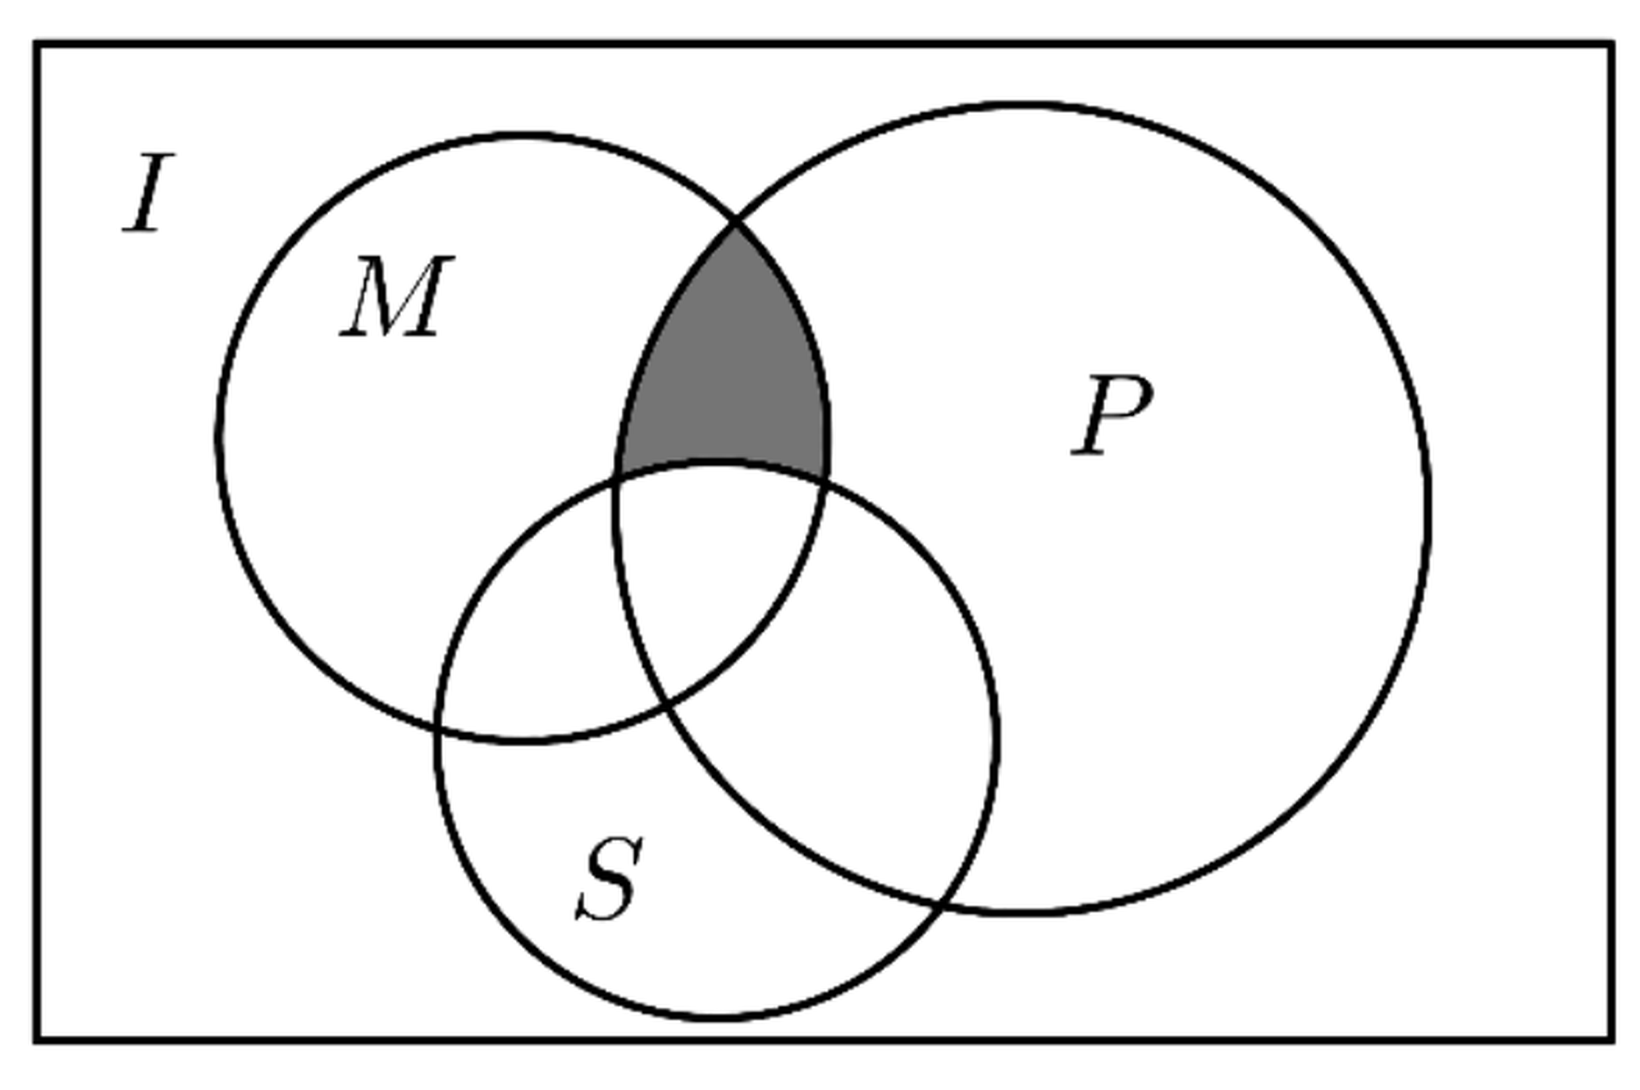
\includegraphics[width=0.42\textwidth]{figures/gao120_q15.png}
\end{center}

\keepwithprev
A. $(M\cap P)\cap S$\qquad\quad B. $(M\cap P)\cap\complement_{I}S$\qquad\quad C. $(M\cup P)\cap S$\qquad\quad D. $\complement_{I}(M\cap P)\cap S$

\ifanswer
\solbegin
\step{由已知中的 $Venn$ 图得阴影部分的元素属于 $M$，属于 $P$，但不属于 $S$，}
\step{所以阴影部分表示的集合为 $(M\cap P)\cap\complement_{I}S$，故选 $B$.}
\solend
\fi

\item 设集合 $P_1=\{x\mid x^2+ax+1>0\}$，$P_2=\{x\mid x^2+ax+2>0\}$，$Q_1=\{x\mid x^2+x+b>0\}$，$Q_2=\{x\mid x^2+2x+b>0\}$，其中 $a$、$b\in\R$，对于下列两个命题：①存在 $a$，$P_1$ 不是 $P_2$ 的子集；②存在 $b$ 使得 $Q_1$ 是 $Q_2$ 的子集. 下列说法正确的是\mbox{（\quad）}

\keepwithprev
A. ①是真命题，②是假命题\qquad\qquad B. ①是假命题，②是真命题

C. ①②都是真命题\qquad\qquad\qquad D. ①②都是假命题

\ifanswer
\solbegin
\step{对于集合 $P_1=\{x\mid x^2+ax+1>0\}$，$P_2=\{x\mid x^2+ax+2>0\}$，}
\step{得当 $m\in P_1$ 时，即 $m^2+am+1>0$，得 $m^2+am+2>0$，}
\step{即有 $m\in P_2$，得对任意 $a$，$P_1$ 是 $P_2$ 的子集，故①错误；}
\step{对于集合 $Q_1=\{x\mid x^2+x+b>0\}$，$Q_2=\{x\mid x^2+2x+b>0\}$，}
\step{当 $b=6$ 时，$Q_1=\{x\mid x^2+x+6>0\}=\R$，$Q_2=\{x\mid x^2+2x+6>0\}=\R$，}
\step{得 $Q_1$ 是 $Q_2$ 的子集，所以存在 $b$，使得 $Q_1$ 是 $Q_2$ 的子集，故②正确；}
\step{故选 $B$.}
\solend
\fi

\end{enumerate}

\bigsec{三、解答题}

\begin{enumerate}
\setcounter{enumi}{16}

\item (1) 已知 $x$、$y$ 都是实数，比较 $x^2+y^2$ 与 $4x-2y-5$ 的大小.

(2) 求解不等式组 $\begin{cases}x^2-4x+3\geqslant0\\\dfrac{x+3}{2x-1}\geqslant2\end{cases}$.

\ifanswer
\solbegin
\step{(1) $(x^2+y^2)-(4x-2y-5)=x^2-4x+y^2+2y+5=(x-2)^2+(y+1)^2\geqslant0$，}
\step{当 $x=2$，$y=-1$ 时，$x^2+y^2=4x-2y-5$.}
\step{当 $x\neq2$ 或 $y\neq-1$ 时，$x^2+y^2>4x-2y-5$.}
\step{(2) 由 $x^2-4x+3\geqslant0$ 得 $(x-1)(x-3)\geqslant0$，所以 $x\leqslant1$ 或 $x\geqslant3$；}
\step{由 $\dfrac{x+3}{2x-1}\geqslant2$，得 $\dfrac{x+3}{2x-1}-2=\dfrac{-3x+5}{2x-1}\geqslant0$，即 $\dfrac{3x-5}{2x-1}\leqslant0$，}
\step{所以 $\begin{cases}(3x-5)(2x-1)\leqslant0\\2x-1\neq0\end{cases}$，解得 $\dfrac12<x\leqslant\dfrac53$，}
\step{所以不等式组的解集是 $\left\{x\,\middle\vert\,\dfrac12<x\leqslant1\right\}$.}
\solend
\fi

\item 已知 $x_1$,$x_2$ 是一元二次方程 $4kx^2-4kx+k+1=0$ 的两个实数根.

(1) 是否存在实数 $k$，$(2x_1-x_2)(x_1-2x_2)=-\dfrac32$ 成立？若存在，求出 $k$ 的值；若不存在，请说明理由.

(2) 求使 $\dfrac{x_1}{x_2}+\dfrac{x_2}{x_1}-2$ 的值为整数的实数 $k$ 的整数值.

\ifanswer
\solbegin
\step{(1) 因为 $x_1$,$x_2$ 是一元二次方程 $4kx^2-4kx+k+1=0$ 的两个实数根，}
\step{所以 $\begin{cases}k\neq0\\16k^2-16k(k+1)\geqslant0\end{cases}$，所以 $k<0$，}
\step{由根与系数的关系得 $x_1+x_2=1$，$x_1x_2=\dfrac{k+1}{4k}$，}
\step{所以 $(2x_1-x_2)(x_1-2x_2)=2(x_1+x_2)^2-9x_1x_2=2-9\times\dfrac{k+1}{4k}=-\dfrac32$，}
\step{解得 $k=\dfrac95$，而 $k<0$，故不存在实数 $k$ 使得 $(2x_1-x_2)(x_1-2x_2)=-\dfrac32$ 成立.}
\step{(2) 由根与系数的关系得 $\dfrac{x_1}{x_2}+\dfrac{x_2}{x_1}-2=\dfrac{(x_1+x_2)^2}{x_1x_2}-4=-\dfrac4{k+1}$，}
\step{因为 $-\dfrac4{k+1}$ 的值为整数，而 $k$ 为整数，所以 $k+1$ 只能取 $\pm1$、$\pm2$、$\pm4$，}
\step{又 $k<0$，所以整数 $k$ 的值为 $-2$ 或 $-3$ 或 $-5$.}
\solend
\fi

\item 2026 年，某市低空经济蓬勃发展，一家物流企业开通“无人机即时配送”服务，并设立配送站. 经市场调研，该站每日配送单量 $y$（单位：单）与每单配送费 $x$（单位：元）满足关系式 $y=4800-200x$（其中 $4<x<24$）. 已知配送站每日的固定成本为 $19200$ 元，每完成一单配送，需支付电费、耗材费、设备保养费等可变成本，每单可变成本为 $4$ 元.

(1) 若要保证配送站每日利润 $W$（单位：元）不为负数，求每单配送费 $x$ 的取值范围；（每日利润 $=$ 每日配送总收入 $-$ 每日可变总成本 $-$ 每日固定成本）

(2) 为提升运力，该站购进一批新型无人机，购机费用为 $32$ 万元. 投入使用后，这批无人机使用 $t(t>0)$ 年的累计维保总费用为 $(2t^2+8t)$ 万元. 请问：这批无人机使用多少年后更新，可以使年平均总费用最低？请求出最低年平均总费用.（年平均总费用 $=$（购机费用 $+$ 维保总费用）$\div$ 使用年数）

\ifanswer
\solbegin
\step{(1) $W=xy-4y-19200=x(4800-200x)-4(4800-200x)-19200$}
\step{$=-200x^2+5600x-38400(4<x<24)$，}
\step{令 $W=-200x^2+5600x-38400\geqslant0$，即 $x^2-28x+192\leqslant0$，}
\step{解得 $12\leqslant x\leqslant16$，因此，要保证配送站每日利润 $W$ 不为负数，}
\step{每单配送费 $x$ 的取值范围为 $[12,16]$；}
\step{(2) 由题意，年平均总费用为 $N=\dfrac{2t^2+8t+32}{t}=2t+\dfrac{32}{t}+8$}
\step{$\geqslant2\sqrt{2t\cdot\dfrac{32}{t}}+8=16+8=24$，当且仅当 $2t=\dfrac{32}{t}$，即 $t=4$ 时取等号，}
\step{则这批无人机使用 $4$ 年后更新，可以使年平均总费用最低，}
\step{最低年平均总费用为 $24$ 万元.}
\solend
\fi

\item 已知 $A,B$，定义集合 $M_{(A,B)}=\{x\mid A<B\}$.

(1) 设 $A=\lvert x-4\rvert$,$B=2x$，求 $M_{(A,B)}$；

(2) 设 $A=ax^2+2ax-4$,$B=2x(x+2)$，当 $M_{(A,B)}=\R$ 时，求 $a$ 的取值范围；

(3) 设 $A=\lvert 2x-b\rvert$,$B=\dfrac{x+4b}{x-1}$,$C=2$，若 $M_{(A,C)}\cap M_{(B,C)}\neq\varnothing$，求 $b$ 的取值范围.

\ifanswer
\solbegin
\step{(1) 由定义，$x\in M_{(A,B)}$ 等价于 $\lvert x-4\rvert<2x$，}
\step{原不等式等价于 $-2x<x-4<2x$，即同时满足 $3x>4$ 与 $x>-4$，}
\step{解得 $x>\dfrac43$，所以 $M_{(A,B)}=\left(\dfrac43,+\infty\right)$.}
\step{(2) 由 $M_{(A,B)}=\R$，得 $ax^2+2ax-4<2x(x+2)$ 对任意 $x\in\R$ 恒成立，}
\step{得 $(a-2)(x+1)^2-a-2<0$.}
\step{当 $a>2$ 时，随着 $(x+1)^2$ 增大，左边可取正值，不符合题意；}
\step{当 $a=2$ 时，左边恒等于 $-4$，符合题意；}
\step{当 $a<2$ 时，左边在 $x=-1$ 处取得最大值 $-a-2$，}
\step{故恒成立的充要条件为 $-a-2<0$，即 $a>-2$；}
\step{综上，$a\in(-2,2]$.}
\step{(3) 由 $\lvert 2x-b\rvert<2$，得 $M_{(A,C)}=\left(\dfrac b2-1,\dfrac b2+1\right)$，记为 $I$.}
\step{由 $\dfrac{x+4b}{x-1}<2$，得 $\dfrac{x-(4b+2)}{x-1}>0$，其中 $x\neq1$.}
\step{①当 $b<-\dfrac14$ 时，$4b+2<1$，故 $M_{(B,C)}=(-\infty,4b+2)\cup(1,+\infty)$.}
\step{此时 $\dfrac b2+1<1$，所以 $I$ 与 $(1,+\infty)$ 没有公共元素.}
\step{两集合交集非空等价于 $\dfrac b2-1<4b+2$，解得 $b>-\dfrac67$.}
\step{因而本种情况得到 $-\dfrac67<b<-\dfrac14$.}
\step{②当 $b=-\dfrac14$ 时，$\dfrac{x+4b}{x-1}=1$，其中 $x\neq1$，故 $M_{(B,C)}=\{x\mid x\neq1\}$.}
\step{此时 $I=\left(-\dfrac98,\dfrac78\right)$，两集合交集非空.}
\step{③当 $b>-\dfrac14$ 时，$4b+2>1$，故 $M_{(B,C)}=(-\infty,1)\cup(4b+2,+\infty)$.}
\step{此时 $4b+2-\left(\dfrac b2+1\right)=\dfrac{7b}{2}+1>\dfrac18>0$，}
\step{所以 $I$ 与 $(4b+2,+\infty)$ 没有公共元素.}
\step{两集合交集非空等价于 $\dfrac b2-1<1$，解得 $b<4$.}
\step{因而本种情况得到 $-\dfrac14<b<4$.}
\step{综上，$b\in\left(-\dfrac67,4\right)$.}
\solend
\fi

\item 破晓同学阅读课外书籍时，发现笛卡尔积是代数和图论中一个很重要的课题. 对于非空数集 $A,B$，定义 $A\otimes B=\{(x,y)\mid x\in A$ 且 $y\in B\}$，将 $A\otimes B$ 称为“$A$ 与 $B$ 的笛卡尔积”.

(1) 若 $A=\{-1,0,1\}$,$B=\{-1,1\}$，求 $A\otimes B$ 和 $B\otimes A$；

(2) 试证明：“$A_1\otimes A_2=A_2\otimes A_1$”是“$A_1=A_2$”的充要条件；

(3) 若集合 $H$ 是有限集，将集合 $H$ 的元素个数记为 $\lvert H\rvert$. 已知 $\lvert A_1\otimes A_2\rvert=m^3(m\in\N^*)$，且存在实数 $a$ 满足 $\sqrt{\dfrac{\lvert A_1\otimes A_1\rvert+\lvert A_2\otimes A_2\rvert}{\lvert A_2\otimes A_1\rvert}}\geqslant a$ 对任意 $m\in\N^*$ 恒成立. 求 $a$ 的取值范围，并指明当 $a$ 取到最值时 $\lvert A_1\rvert$ 和 $\lvert A_2\rvert$ 满足的关系式及 $m$ 应满足的条件.

\ifanswer
\solbegin
\step{(1) 由题意得 $A\otimes B=\{(-1,-1),(-1,1),(0,-1),(0,1),(1,-1),(1,1)\}$，}
\step{$B\otimes A=\{(-1,-1),(-1,0),(-1,1),(1,-1),(1,0),(1,1)\}$；}
\step{(2) 若 $A_1=A_2$，设 $A_1=A_2=A$，}
\step{由定义得 $A_1\otimes A_2=\{(a,b)\mid a\in A$ 且 $b\in A\}=A_2\otimes A_1$，}
\step{所以“$A_1\otimes A_2=A_2\otimes A_1$”是“$A_1=A_2$”的必要条件；}
\step{若 $A_1\otimes A_2=A_2\otimes A_1$，对任意 $(a,b)\in A_1\otimes A_2$，均有 $(a,b)\in A_2\otimes A_1$，}
\step{即对任意 $a\in A_1,b\in A_2$，均有 $a\in A_2,b\in A_1$，}
\step{由任意性得 $A_1\subseteq A_2,A_2\subseteq A_1$，则 $A_1=A_2$，}
\step{所以“$A_1\otimes A_2=A_2\otimes A_1$”是“$A_1=A_2$”的充分条件；}
\step{综上所述，“$A_1\otimes A_2=A_2\otimes A_1$”是“$A_1=A_2$”的充要条件.}
\step{(3) 设 $\lvert A_1\rvert=c$,$\lvert A_2\rvert=d$,$c,d\in\N^*$，}
\step{则 $\lvert A_1\otimes A_2\rvert=\lvert A_2\otimes A_1\rvert=cd=m^3$,$\lvert A_1\otimes A_1\rvert=c^2$,$\lvert A_2\otimes A_2\rvert=d^2$，}
\step{得 $\sqrt{\dfrac{\lvert A_1\otimes A_1\rvert+\lvert A_2\otimes A_2\rvert}{\lvert A_2\otimes A_1\rvert}}=\sqrt{\dfrac{c^2+d^2}{cd}}=\sqrt{\dfrac cd+\dfrac dc}\geqslant\sqrt{2\sqrt{\dfrac cd\cdot\dfrac dc}}=\sqrt2$，}
\step{当且仅当 $\dfrac cd=\dfrac dc$，即 $c=d$ 时取等号，所以实数 $a$ 的取值范围是 $(-\infty,\sqrt2]$.}
\step{若 $a$ 取到最大值，则 $c=d$，即 $\lvert A_1\rvert=\lvert A_2\rvert$，得 $c^2=m^3$，}
\step{即 $c=\sqrt{m^3}=(\sqrt m)^3\in\N^*$，所以 $m=k^2,k\in\N^*$.}
\solend
\fi

\end{enumerate}

\end{document}
"
%
% 原始材料：微信公众号“魔都数学加油站”文章，作者破晓，2026-11-08 21:35 发布；
% 连载“27学年高一120”，原文标题“27学年高一120——2026-2027年上海市松江二中高一上10月月考”；
% 原文链接：https://mp.weixin.qq.com/s/hgDkaZX9M_IKhmr7CjQc1A。
% 正文为 10 张 PNG 页（第 8、10 页 2560×3620，其余 4762×6735），
% 题目下印有【解析】或【答案】，为讲评版。
% 题目、解析均据原图转录；卷面红色水印及公众号页脚未录入。
% 全卷 1 张插图：第 15 题的三集合 Venn 图（原卷印在题干右侧，本稿移至题干之后，
% 取原卷截图 2× LANCZOS 放大，见 figures/gao120_q15.png）。
%
% 卷首标题：原卷印作“2026-2027 年松江二中高一上 10 月月考”（公众号标题中的“上海市”
% 卷面标题行没有，本稿照卷面），年份区间按全稿惯例排 en dash；原卷未印副标题，本稿按题目内容
% 标为“集合与常用逻辑用语、不等式”（与 110／111／113／116／118 同）。
%
% 与原卷的排版差异：
%   ① 原文从第 3 题起，填空题编号为 3—12、选择题为 13—16、解答题为 17—21，本稿保留原题号；
%   ② 原卷每题下直接印【解析】／【答案】，本稿按全稿惯例置于答案版；第 3 题只印【答案】、
%      第 13、14 题把答案印在题干括号内且无【解析】，均另提 \ans{}；其余选择题答案在
%      解析末句“故选 …”，括号内留空；
%   ③ 原卷未印副标题，本稿按“知识模块”口径补出；
%   ④ 原卷填空横线按全稿惯例排为 \blankline[4.4em]；选择题括号排 \mbox{（\quad）}、
%      选项段前按惯例加 \keepwithprev；解答题不留作答区（原卷为讲评版，与 109—119 同）；
%   ⑤ 原卷数集排斜体 $R$、$N^*$，按全稿惯例改 \R、\N^*；绝对值排 \lvert…\rvert，
%      集合描述竖线排 \mid；补集记号照原卷排 \complement_I。
%
% 判别式字形：第 9 题解析作 $\triangle$（等边、扁），照录 \triangle。
%
% 子集符号：第 4 题题干与解析的 $A\subseteq B$、第 21 题 (2) 的 $A_1\subseteq A_2$ 印有下划线，
%   照录 \subseteq。
%
% 原卷存疑照录：第 12 题题干 $S=\{82,83,84,85,86,87,89\}$ 跳过 $88$ 只列 7 个数，
%   与其“8 种不同的值”自洽（不含 $88$），照录；第 19 题 (1) 的 $W$ 表达式
%   $x(4800-200x)-4(4800-200x)-19200$ 与最后结果 $[12,16]$ 一致。
%
% 行数核对：逐题数 \step 条数，合计 115 条（Q3：0；Q4：4；Q5：2；Q6：5；Q7：4；
% Q8：2；Q9：5；Q10：3；Q11：6；Q12：11；Q13：0；Q14：0；Q15：2；Q16：7；
% Q17：7；Q18：8；Q19：9；Q20：24；Q21：16），与原卷印刷行逐题相等
% （cases 块作一个印刷行计）。第 3 题只印【答案】、第 13、14 题括号内印答案且无解析，
% 均提 \ans{}，不计入 \step 账。
%
\documentclass[a4paper,11pt]{article}
\usepackage{common}

\begin{document}

\examtitlest[3]{2026--2027 年松江二中高一上 10 月月考}{集合与常用逻辑用语、不等式}

\bigsec{一、填空题}

\begin{enumerate}
\setcounter{enumi}{2}

\item 集合 $A=\{(x,y)\mid x+y=8\}$,$B=\{(x,y)\mid xy=12\}$，求 $A\cap B=$\blankline[4.4em].

\ifanswer
\ans{$\{(2,6),(6,2)\}$}
\fi

\item 设集合 $A=\{0,-a\}$,$B=\{1,a-2,2a-2\}$，若 $A\subseteq B$，则 $a=$\blankline[4.4em].

\ifanswer
\solbegin
\step{因为 $A\subseteq B$，}
\step{若 $a-2=0$，解得 $a=2$，此时 $A=\{0,-2\}$,$B=\{1,0,2\}$，不符合题意；}
\step{若 $2a-2=0$，解得 $a=1$，此时 $A=\{0,-1\}$,$B=\{1,-1,0\}$，符合题意；}
\step{综上所述，$a=1$.}
\solend
\fi

\item 设 $\alpha:0<x<a(a>0)$,$\beta:x<8-3a$，若 $\alpha$ 是 $\beta$ 的充分条件，则实数 $a$ 的取值范围是\blankline[4.4em].

\ifanswer
\solbegin
\step{由 $\alpha$ 是 $\beta$ 的充分条件得，$x\in(0,a)\Rightarrow x\in(-\infty,8-3a)$，}
\step{所以 $0<a\leqslant8-3a$，解得 $0<a\leqslant2$.}
\solend
\fi

\item 关于 $x$ 的不等式 $ax-b>0$ 的解集为 $(-\infty,1)$，则不等式 $\dfrac{x-2}{ax+b}<0$ 的解集为\blankline[4.4em].

\ifanswer
\solbegin
\step{因为关于 $x$ 的不等式 $ax-b>0$ 的解集为 $(-\infty,1)$，}
\step{所以 $a<0$ 且 $\dfrac ba=1$，则 $b=a$，}
\step{所以不等式 $\dfrac{x-2}{ax+b}<0$，即 $\dfrac{x-2}{ax+a}<0$，即 $\dfrac{x-2}{x+1}>0$，}
\step{等价于 $(x+1)(x-2)>0$，解得 $x>2$ 或 $x<-1$，}
\step{即解集为 $(-\infty,-1)\cup(2,+\infty)$.}
\solend
\fi

\item 若正实数 $x$、$y$ 满足 $2x+y+8xy=2$，则 $xy$ 的最大值为\blankline[4.4em].

\ifanswer
\solbegin
\step{因为正实数 $x$、$y$ 满足 $2x+y+8xy=2$，}
\step{所以 $2-8xy=2x+y\geqslant2\sqrt{2xy}$，}
\step{当且仅当 $y=2x$，即 $x=\dfrac14$，$y=\dfrac12$ 时取等号，解得 $0<xy\leqslant\dfrac18$，}
\step{故 $xy$ 的最大值为 $\dfrac18$.}
\solend
\fi

\item 已知 $1<a<3$，$-5<b<-2$，则 $\dfrac ab$ 的取值范围是\blankline[4.4em].

\ifanswer
\solbegin
\step{因为 $-5<b<-2$，所以 $2<-b<5$，$\dfrac15<-\dfrac1b<\dfrac12$，又 $1<a<3$，}
\step{得 $\dfrac15<-\dfrac ab<\dfrac32$，则 $-\dfrac32<\dfrac ab<-\dfrac15$，故 $\dfrac ab$ 的取值范围是 $\left(-\dfrac32,-\dfrac15\right)$.}
\solend
\fi

\item 若关于 $x$、$y$ 的方程组 $\begin{cases}y-kx-2=0\\y^2-4x-2y+1=0\end{cases}$ 的解集中只有一个元素，则实数 $k$ 的值为\blankline[4.4em].

\ifanswer
\solbegin
\step{由 $\begin{cases}y-kx-2=0\\y^2-4x-2y+1=0\end{cases}$ 消去 $y$ 整理得 $k^2x^2+(2k-4)x+1=0$.}
\step{当 $k\neq0$ 时，则 $\triangle=(2k-4)^2-4k^2=0$，解得 $k=1$，}
\step{此时方程组的解为 $\begin{cases}x=1\\y=3\end{cases}$，符合题意；}
\step{当 $k=0$ 时，解得 $x=\dfrac14$，此时方程组的解为 $\begin{cases}x=\dfrac14\\y=2\end{cases}$，符合题意；}
\step{综上，$k=0$ 或 $k=1$.}
\solend
\fi

\item 若集合 $A=\{0,1\}$，$B=\{x\mid x^2-mx-m>0,x\in\R\}$，且 $A\cap B=\{1\}$，则实数 $m$ 的取值范围为\blankline[4.4em].

\ifanswer
\solbegin
\step{因为集合 $A=\{0,1\}$，$B=\{x\mid x^2-mx-m>0,x\in\R\}$，且 $A\cap B=\{1\}$，}
\step{则 $1\in B$ 且 $0\notin B$，所以 $\begin{cases}1-m-m>0\\-m\leqslant0\end{cases}$，解得 $0\leqslant m<\dfrac12$，}
\step{所以实数 $m$ 的取值范围是 $\left[0,\dfrac12\right)$.}
\solend
\fi

\item 从集合 $U=\{a,b,c,d\}$ 的子集中选出两个不同的子集，需同时满足以下两个条件：(1) $a$、$b$ 都至少属于其中一个集合；(2) 对选出的两个子集，其中一个集合为另一个的子集，那么共有\blankline[4.4em]种不同的选法.

\ifanswer
\solbegin
\step{不妨设元素少的为 $A$，元素多的为 $B$，则 $B$ 必包含有 $a$、$b$；$A$ 为 $B$ 的真子集，}
\step{若 $B=\{a,b\}$，$A$ 为 $B$ 的真子集，共 $2^2-1=3$ 种，}
\step{若 $B=\{a,b,c\}$，$A$ 为 $B$ 的真子集，共 $2^3-1=7$ 种，}
\step{若 $B=\{a,b,d\}$，$A$ 为 $B$ 的真子集，共 $2^3-1=7$ 种，}
\step{若 $B=\{a,b,c,d\}$，$A$ 为 $B$ 的真子集，共 $2^4-1=15$ 种，}
\step{共有 $3+7+7+15=32$ 种.}
\solend
\fi

\item 已知 $a_1$、$a_2$、$\cdots$、$a_8$ 是 $8$ 个正整数，记 $S=\{a_{i_1}+a_{i_2}+\cdots+a_{i_7}\mid 1\leqslant i_1<i_2<\cdots<i_7\leqslant8\}$，其中 $i_1$、$i_2$、$\cdots$、$i_7\in\N^*$，若 $S=\{82,83,84,85,86,87,89\}$，则这 $8$ 个正整数中的最大数与最小数的积为\blankline[4.4em].

\ifanswer
\solbegin
\step{由题意得从 $8$ 个数中任取 $7$ 个数的和共有 $C_8^7=8$ 种不同的值，}
\step{但是 $82$，$83$，$84$，$85$，$86$，$87$，$89$ 只有 $7$ 个数，}
\step{得必有两种 $7$ 个数的和相等，设这个和为 $t(82\leqslant t\leqslant89)$，}
\step{令 $T=\sum\limits_{i=1}^{8}a_i$，那么，任取 $7$ 个数的和就等于 $T-a_i$，$i=1,2,\cdots,8$，}
\step{这 $8$ 个取值和的集合为 $S$，$S=\{T-a_1,T-a_2,\cdots,T-a_8\}$，}
\step{则 $\sum\limits_{i=1}^{8}(T-a_i)=8T-T=7T=82+83+84+85+86+87+89+t=596+t$.}
\step{因为 $T$ 为整数，所以 $596+t$ 是 $7$ 的倍数，}
\step{由 $596=7\times85+1$ 得 $1+t$ 是 $7$ 的倍数，}
\step{再因为 $82\leqslant t\leqslant89$，所以 $t=83$，得 $T=97$.}
\step{因此 $a_1$、$a_2$、$\cdots$、$a_8$ 中最大数为 $97-82=15$，最小数为 $97-89=8$，}
\step{因此，它们的积为 $120$.}
\solend
\fi

\end{enumerate}

\bigsec{二、选择题}

\begin{enumerate}
\setcounter{enumi}{12}

\item 已知 $a>b>0$，$c\in\R$，则下列不等式不一定成立的是\mbox{（\quad）}% 原卷把答案“$B$”印在题干括号内、无【解析】

\keepwithprev
A. $a-c>b-c$\qquad\quad B. $ac>bc$\qquad\quad C. $\dfrac1a<\dfrac1b$\qquad\quad D. $\dfrac{a+b}{2}>\sqrt{ab}$

\ifanswer
\ans{$B$}
\fi

\item 命题“对任意的 $x\in\R,x^3-x^2+1\leqslant0$”的否定是\mbox{（\quad）}% 原卷把答案“$C$”印在题干括号内、无【解析】

\keepwithprev
A. 不存在 $x\in\R,x^3-x^2+1\leqslant0$\qquad B. 存在 $x\in\R,x^3-x^2+1\leqslant0$

C. 存在 $x\in\R,x^3-x^2+1>0$\qquad\quad D. 对任意的 $x\in\R,x^3-x^2+1>0$

\ifanswer
\ans{$C$}
\fi

% 第 15 题是“题干 + 图 + 选项”约 6.5cm 的一整块，\keepwithprev 只挡得住“图—选项”，
% 挡不住夹在中间的图——实测断点落在题干之后（切页审计 A 类）。故照 高一30／高一26 成例
% 在题前先量一次页高，不够就把整块一起挪到次页。
\needvspace{7cm}
\item 如图，$I$ 是全集，$M$、$P$、$S$ 是 $I$ 的三个子集，则阴影部分所表示的集合是\mbox{（\quad）}

\begin{center}
% 图取原卷截图（第 4 页题干右侧）、2× LANCZOS 放大，本稿移至题干之后
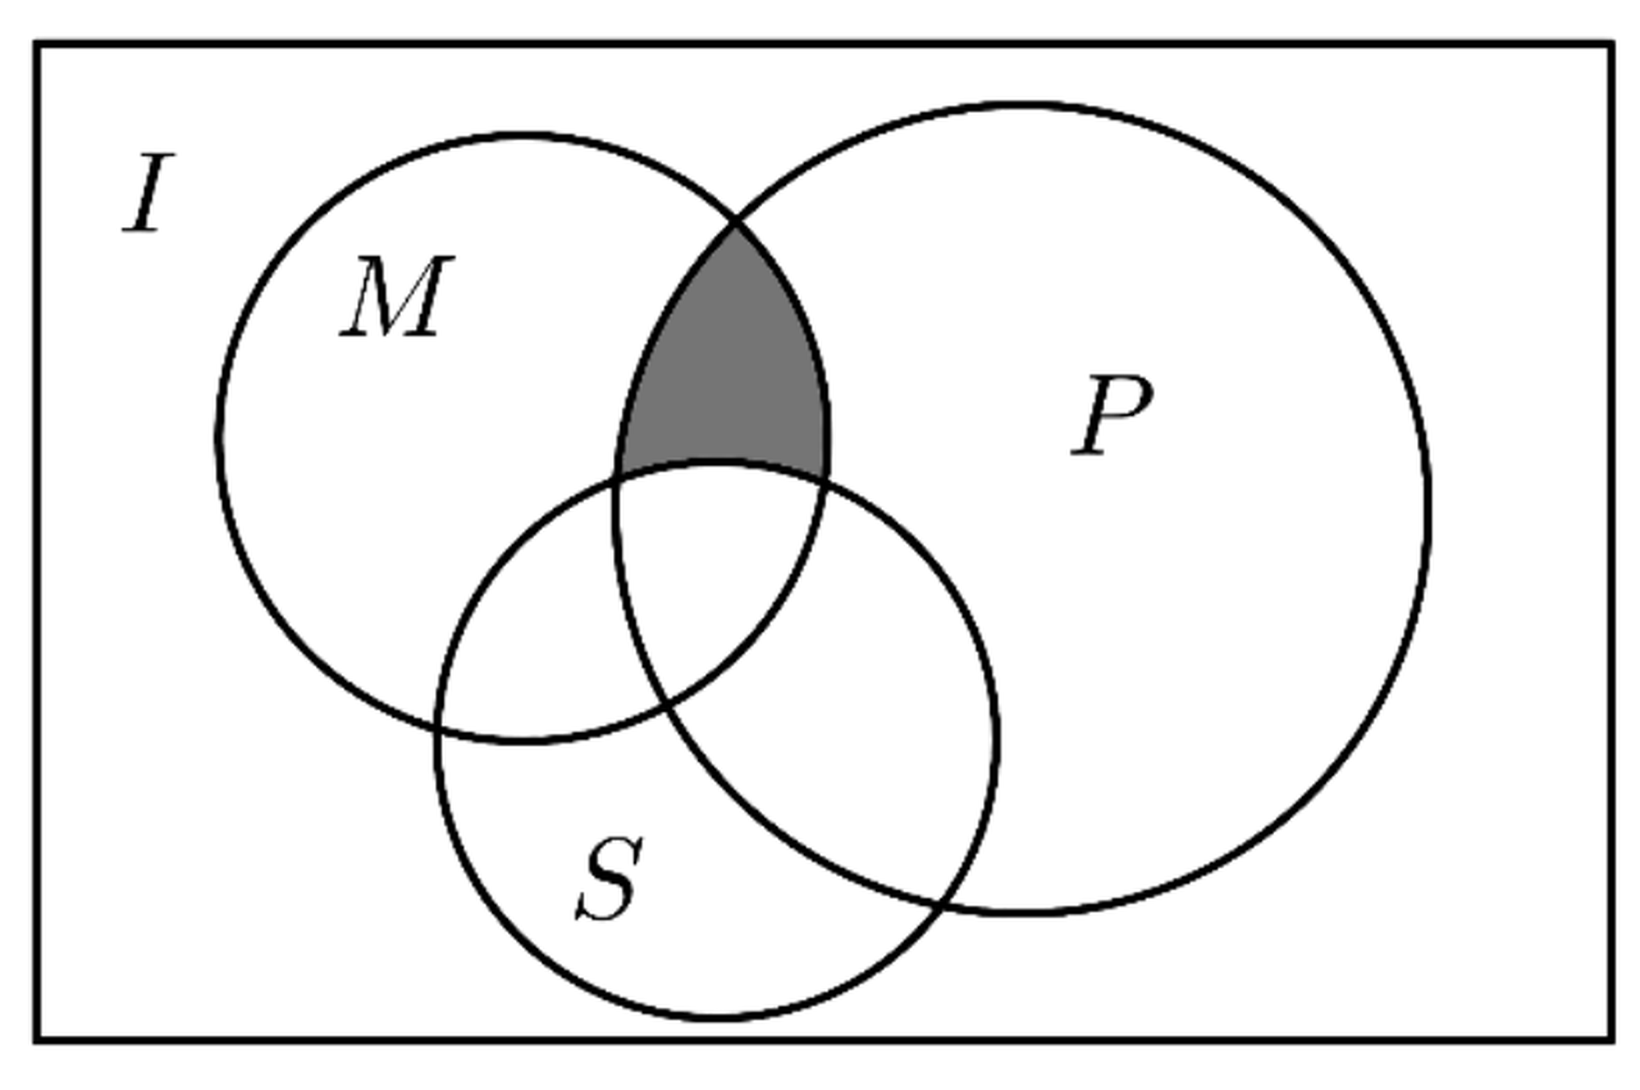
\includegraphics[width=0.42\textwidth]{figures/gao120_q15.png}
\end{center}

\keepwithprev
A. $(M\cap P)\cap S$\qquad\quad B. $(M\cap P)\cap\complement_{I}S$\qquad\quad C. $(M\cup P)\cap S$\qquad\quad D. $\complement_{I}(M\cap P)\cap S$

\ifanswer
\solbegin
\step{由已知中的 $Venn$ 图得阴影部分的元素属于 $M$，属于 $P$，但不属于 $S$，}
\step{所以阴影部分表示的集合为 $(M\cap P)\cap\complement_{I}S$，故选 $B$.}
\solend
\fi

\item 设集合 $P_1=\{x\mid x^2+ax+1>0\}$，$P_2=\{x\mid x^2+ax+2>0\}$，$Q_1=\{x\mid x^2+x+b>0\}$，$Q_2=\{x\mid x^2+2x+b>0\}$，其中 $a$、$b\in\R$，对于下列两个命题：①存在 $a$，$P_1$ 不是 $P_2$ 的子集；②存在 $b$ 使得 $Q_1$ 是 $Q_2$ 的子集. 下列说法正确的是\mbox{（\quad）}

\keepwithprev
A. ①是真命题，②是假命题\qquad\qquad B. ①是假命题，②是真命题

C. ①②都是真命题\qquad\qquad\qquad D. ①②都是假命题

\ifanswer
\solbegin
\step{对于集合 $P_1=\{x\mid x^2+ax+1>0\}$，$P_2=\{x\mid x^2+ax+2>0\}$，}
\step{得当 $m\in P_1$ 时，即 $m^2+am+1>0$，得 $m^2+am+2>0$，}
\step{即有 $m\in P_2$，得对任意 $a$，$P_1$ 是 $P_2$ 的子集，故①错误；}
\step{对于集合 $Q_1=\{x\mid x^2+x+b>0\}$，$Q_2=\{x\mid x^2+2x+b>0\}$，}
\step{当 $b=6$ 时，$Q_1=\{x\mid x^2+x+6>0\}=\R$，$Q_2=\{x\mid x^2+2x+6>0\}=\R$，}
\step{得 $Q_1$ 是 $Q_2$ 的子集，所以存在 $b$，使得 $Q_1$ 是 $Q_2$ 的子集，故②正确；}
\step{故选 $B$.}
\solend
\fi

\end{enumerate}

\bigsec{三、解答题}

\begin{enumerate}
\setcounter{enumi}{16}

\item (1) 已知 $x$、$y$ 都是实数，比较 $x^2+y^2$ 与 $4x-2y-5$ 的大小.

(2) 求解不等式组 $\begin{cases}x^2-4x+3\geqslant0\\\dfrac{x+3}{2x-1}\geqslant2\end{cases}$.

\ifanswer
\solbegin
\step{(1) $(x^2+y^2)-(4x-2y-5)=x^2-4x+y^2+2y+5=(x-2)^2+(y+1)^2\geqslant0$，}
\step{当 $x=2$，$y=-1$ 时，$x^2+y^2=4x-2y-5$.}
\step{当 $x\neq2$ 或 $y\neq-1$ 时，$x^2+y^2>4x-2y-5$.}
\step{(2) 由 $x^2-4x+3\geqslant0$ 得 $(x-1)(x-3)\geqslant0$，所以 $x\leqslant1$ 或 $x\geqslant3$；}
\step{由 $\dfrac{x+3}{2x-1}\geqslant2$，得 $\dfrac{x+3}{2x-1}-2=\dfrac{-3x+5}{2x-1}\geqslant0$，即 $\dfrac{3x-5}{2x-1}\leqslant0$，}
\step{所以 $\begin{cases}(3x-5)(2x-1)\leqslant0\\2x-1\neq0\end{cases}$，解得 $\dfrac12<x\leqslant\dfrac53$，}
\step{所以不等式组的解集是 $\left\{x\,\middle\vert\,\dfrac12<x\leqslant1\right\}$.}
\solend
\fi

\item 已知 $x_1$,$x_2$ 是一元二次方程 $4kx^2-4kx+k+1=0$ 的两个实数根.

(1) 是否存在实数 $k$，$(2x_1-x_2)(x_1-2x_2)=-\dfrac32$ 成立？若存在，求出 $k$ 的值；若不存在，请说明理由.

(2) 求使 $\dfrac{x_1}{x_2}+\dfrac{x_2}{x_1}-2$ 的值为整数的实数 $k$ 的整数值.

\ifanswer
\solbegin
\step{(1) 因为 $x_1$,$x_2$ 是一元二次方程 $4kx^2-4kx+k+1=0$ 的两个实数根，}
\step{所以 $\begin{cases}k\neq0\\16k^2-16k(k+1)\geqslant0\end{cases}$，所以 $k<0$，}
\step{由根与系数的关系得 $x_1+x_2=1$，$x_1x_2=\dfrac{k+1}{4k}$，}
\step{所以 $(2x_1-x_2)(x_1-2x_2)=2(x_1+x_2)^2-9x_1x_2=2-9\times\dfrac{k+1}{4k}=-\dfrac32$，}
\step{解得 $k=\dfrac95$，而 $k<0$，故不存在实数 $k$ 使得 $(2x_1-x_2)(x_1-2x_2)=-\dfrac32$ 成立.}
\step{(2) 由根与系数的关系得 $\dfrac{x_1}{x_2}+\dfrac{x_2}{x_1}-2=\dfrac{(x_1+x_2)^2}{x_1x_2}-4=-\dfrac4{k+1}$，}
\step{因为 $-\dfrac4{k+1}$ 的值为整数，而 $k$ 为整数，所以 $k+1$ 只能取 $\pm1$、$\pm2$、$\pm4$，}
\step{又 $k<0$，所以整数 $k$ 的值为 $-2$ 或 $-3$ 或 $-5$.}
\solend
\fi

\item 2026 年，某市低空经济蓬勃发展，一家物流企业开通“无人机即时配送”服务，并设立配送站. 经市场调研，该站每日配送单量 $y$（单位：单）与每单配送费 $x$（单位：元）满足关系式 $y=4800-200x$（其中 $4<x<24$）. 已知配送站每日的固定成本为 $19200$ 元，每完成一单配送，需支付电费、耗材费、设备保养费等可变成本，每单可变成本为 $4$ 元.

(1) 若要保证配送站每日利润 $W$（单位：元）不为负数，求每单配送费 $x$ 的取值范围；（每日利润 $=$ 每日配送总收入 $-$ 每日可变总成本 $-$ 每日固定成本）

(2) 为提升运力，该站购进一批新型无人机，购机费用为 $32$ 万元. 投入使用后，这批无人机使用 $t(t>0)$ 年的累计维保总费用为 $(2t^2+8t)$ 万元. 请问：这批无人机使用多少年后更新，可以使年平均总费用最低？请求出最低年平均总费用.（年平均总费用 $=$（购机费用 $+$ 维保总费用）$\div$ 使用年数）

\ifanswer
\solbegin
\step{(1) $W=xy-4y-19200=x(4800-200x)-4(4800-200x)-19200$}
\step{$=-200x^2+5600x-38400(4<x<24)$，}
\step{令 $W=-200x^2+5600x-38400\geqslant0$，即 $x^2-28x+192\leqslant0$，}
\step{解得 $12\leqslant x\leqslant16$，因此，要保证配送站每日利润 $W$ 不为负数，}
\step{每单配送费 $x$ 的取值范围为 $[12,16]$；}
\step{(2) 由题意，年平均总费用为 $N=\dfrac{2t^2+8t+32}{t}=2t+\dfrac{32}{t}+8$}
\step{$\geqslant2\sqrt{2t\cdot\dfrac{32}{t}}+8=16+8=24$，当且仅当 $2t=\dfrac{32}{t}$，即 $t=4$ 时取等号，}
\step{则这批无人机使用 $4$ 年后更新，可以使年平均总费用最低，}
\step{最低年平均总费用为 $24$ 万元.}
\solend
\fi

\item 已知 $A,B$，定义集合 $M_{(A,B)}=\{x\mid A<B\}$.

(1) 设 $A=\lvert x-4\rvert$,$B=2x$，求 $M_{(A,B)}$；

(2) 设 $A=ax^2+2ax-4$,$B=2x(x+2)$，当 $M_{(A,B)}=\R$ 时，求 $a$ 的取值范围；

(3) 设 $A=\lvert 2x-b\rvert$,$B=\dfrac{x+4b}{x-1}$,$C=2$，若 $M_{(A,C)}\cap M_{(B,C)}\neq\varnothing$，求 $b$ 的取值范围.

\ifanswer
\solbegin
\step{(1) 由定义，$x\in M_{(A,B)}$ 等价于 $\lvert x-4\rvert<2x$，}
\step{原不等式等价于 $-2x<x-4<2x$，即同时满足 $3x>4$ 与 $x>-4$，}
\step{解得 $x>\dfrac43$，所以 $M_{(A,B)}=\left(\dfrac43,+\infty\right)$.}
\step{(2) 由 $M_{(A,B)}=\R$，得 $ax^2+2ax-4<2x(x+2)$ 对任意 $x\in\R$ 恒成立，}
\step{得 $(a-2)(x+1)^2-a-2<0$.}
\step{当 $a>2$ 时，随着 $(x+1)^2$ 增大，左边可取正值，不符合题意；}
\step{当 $a=2$ 时，左边恒等于 $-4$，符合题意；}
\step{当 $a<2$ 时，左边在 $x=-1$ 处取得最大值 $-a-2$，}
\step{故恒成立的充要条件为 $-a-2<0$，即 $a>-2$；}
\step{综上，$a\in(-2,2]$.}
\step{(3) 由 $\lvert 2x-b\rvert<2$，得 $M_{(A,C)}=\left(\dfrac b2-1,\dfrac b2+1\right)$，记为 $I$.}
\step{由 $\dfrac{x+4b}{x-1}<2$，得 $\dfrac{x-(4b+2)}{x-1}>0$，其中 $x\neq1$.}
\step{①当 $b<-\dfrac14$ 时，$4b+2<1$，故 $M_{(B,C)}=(-\infty,4b+2)\cup(1,+\infty)$.}
\step{此时 $\dfrac b2+1<1$，所以 $I$ 与 $(1,+\infty)$ 没有公共元素.}
\step{两集合交集非空等价于 $\dfrac b2-1<4b+2$，解得 $b>-\dfrac67$.}
\step{因而本种情况得到 $-\dfrac67<b<-\dfrac14$.}
\step{②当 $b=-\dfrac14$ 时，$\dfrac{x+4b}{x-1}=1$，其中 $x\neq1$，故 $M_{(B,C)}=\{x\mid x\neq1\}$.}
\step{此时 $I=\left(-\dfrac98,\dfrac78\right)$，两集合交集非空.}
\step{③当 $b>-\dfrac14$ 时，$4b+2>1$，故 $M_{(B,C)}=(-\infty,1)\cup(4b+2,+\infty)$.}
\step{此时 $4b+2-\left(\dfrac b2+1\right)=\dfrac{7b}{2}+1>\dfrac18>0$，}
\step{所以 $I$ 与 $(4b+2,+\infty)$ 没有公共元素.}
\step{两集合交集非空等价于 $\dfrac b2-1<1$，解得 $b<4$.}
\step{因而本种情况得到 $-\dfrac14<b<4$.}
\step{综上，$b\in\left(-\dfrac67,4\right)$.}
\solend
\fi

\item 破晓同学阅读课外书籍时，发现笛卡尔积是代数和图论中一个很重要的课题. 对于非空数集 $A,B$，定义 $A\otimes B=\{(x,y)\mid x\in A$ 且 $y\in B\}$，将 $A\otimes B$ 称为“$A$ 与 $B$ 的笛卡尔积”.

(1) 若 $A=\{-1,0,1\}$,$B=\{-1,1\}$，求 $A\otimes B$ 和 $B\otimes A$；

(2) 试证明：“$A_1\otimes A_2=A_2\otimes A_1$”是“$A_1=A_2$”的充要条件；

(3) 若集合 $H$ 是有限集，将集合 $H$ 的元素个数记为 $\lvert H\rvert$. 已知 $\lvert A_1\otimes A_2\rvert=m^3(m\in\N^*)$，且存在实数 $a$ 满足 $\sqrt{\dfrac{\lvert A_1\otimes A_1\rvert+\lvert A_2\otimes A_2\rvert}{\lvert A_2\otimes A_1\rvert}}\geqslant a$ 对任意 $m\in\N^*$ 恒成立. 求 $a$ 的取值范围，并指明当 $a$ 取到最值时 $\lvert A_1\rvert$ 和 $\lvert A_2\rvert$ 满足的关系式及 $m$ 应满足的条件.

\ifanswer
\solbegin
\step{(1) 由题意得 $A\otimes B=\{(-1,-1),(-1,1),(0,-1),(0,1),(1,-1),(1,1)\}$，}
\step{$B\otimes A=\{(-1,-1),(-1,0),(-1,1),(1,-1),(1,0),(1,1)\}$；}
\step{(2) 若 $A_1=A_2$，设 $A_1=A_2=A$，}
\step{由定义得 $A_1\otimes A_2=\{(a,b)\mid a\in A$ 且 $b\in A\}=A_2\otimes A_1$，}
\step{所以“$A_1\otimes A_2=A_2\otimes A_1$”是“$A_1=A_2$”的必要条件；}
\step{若 $A_1\otimes A_2=A_2\otimes A_1$，对任意 $(a,b)\in A_1\otimes A_2$，均有 $(a,b)\in A_2\otimes A_1$，}
\step{即对任意 $a\in A_1,b\in A_2$，均有 $a\in A_2,b\in A_1$，}
\step{由任意性得 $A_1\subseteq A_2,A_2\subseteq A_1$，则 $A_1=A_2$，}
\step{所以“$A_1\otimes A_2=A_2\otimes A_1$”是“$A_1=A_2$”的充分条件；}
\step{综上所述，“$A_1\otimes A_2=A_2\otimes A_1$”是“$A_1=A_2$”的充要条件.}
\step{(3) 设 $\lvert A_1\rvert=c$,$\lvert A_2\rvert=d$,$c,d\in\N^*$，}
\step{则 $\lvert A_1\otimes A_2\rvert=\lvert A_2\otimes A_1\rvert=cd=m^3$,$\lvert A_1\otimes A_1\rvert=c^2$,$\lvert A_2\otimes A_2\rvert=d^2$，}
\step{得 $\sqrt{\dfrac{\lvert A_1\otimes A_1\rvert+\lvert A_2\otimes A_2\rvert}{\lvert A_2\otimes A_1\rvert}}=\sqrt{\dfrac{c^2+d^2}{cd}}=\sqrt{\dfrac cd+\dfrac dc}\geqslant\sqrt{2\sqrt{\dfrac cd\cdot\dfrac dc}}=\sqrt2$，}
\step{当且仅当 $\dfrac cd=\dfrac dc$，即 $c=d$ 时取等号，所以实数 $a$ 的取值范围是 $(-\infty,\sqrt2]$.}
\step{若 $a$ 取到最大值，则 $c=d$，即 $\lvert A_1\rvert=\lvert A_2\rvert$，得 $c^2=m^3$，}
\step{即 $c=\sqrt{m^3}=(\sqrt m)^3\in\N^*$，所以 $m=k^2,k\in\N^*$.}
\solend
\fi

\end{enumerate}

\end{document}
"
%
% 原始材料：微信公众号“魔都数学加油站”文章，作者破晓，2026-11-08 21:35 发布；
% 连载“27学年高一120”，原文标题“27学年高一120——2026-2027年上海市松江二中高一上10月月考”；
% 原文链接：https://mp.weixin.qq.com/s/hgDkaZX9M_IKhmr7CjQc1A。
% 正文为 10 张 PNG 页（第 8、10 页 2560×3620，其余 4762×6735），
% 题目下印有【解析】或【答案】，为讲评版。
% 题目、解析均据原图转录；卷面红色水印及公众号页脚未录入。
% 全卷 1 张插图：第 15 题的三集合 Venn 图（原卷印在题干右侧，本稿移至题干之后，
% 取原卷截图 2× LANCZOS 放大，见 figures/gao120_q15.png）。
%
% 卷首标题：原卷印作“2026-2027 年松江二中高一上 10 月月考”（公众号标题中的“上海市”
% 卷面标题行没有，本稿照卷面），年份区间按全稿惯例排 en dash；原卷未印副标题，本稿按题目内容
% 标为“集合与常用逻辑用语、不等式”（与 110／111／113／116／118 同）。
%
% 与原卷的排版差异：
%   ① 原文从第 3 题起，填空题编号为 3—12、选择题为 13—16、解答题为 17—21，本稿保留原题号；
%   ② 原卷每题下直接印【解析】／【答案】，本稿按全稿惯例置于答案版；第 3 题只印【答案】、
%      第 13、14 题把答案印在题干括号内且无【解析】，均另提 \ans{}；其余选择题答案在
%      解析末句“故选 …”，括号内留空；
%   ③ 原卷未印副标题，本稿按“知识模块”口径补出；
%   ④ 原卷填空横线按全稿惯例排为 \blankline[4.4em]；选择题括号排 \mbox{（\quad）}、
%      选项段前按惯例加 \keepwithprev；解答题不留作答区（原卷为讲评版，与 109—119 同）；
%   ⑤ 原卷数集排斜体 $R$、$N^*$，按全稿惯例改 \R、\N^*；绝对值排 \lvert…\rvert，
%      集合描述竖线排 \mid；补集记号照原卷排 \complement_I。
%
% 判别式字形：第 9 题解析作 $\triangle$（等边、扁），照录 \triangle。
%
% 子集符号：第 4 题题干与解析的 $A\subseteq B$、第 21 题 (2) 的 $A_1\subseteq A_2$ 印有下划线，
%   照录 \subseteq。
%
% 原卷存疑照录：第 12 题题干 $S=\{82,83,84,85,86,87,89\}$ 跳过 $88$ 只列 7 个数，
%   与其“8 种不同的值”自洽（不含 $88$），照录；第 19 题 (1) 的 $W$ 表达式
%   $x(4800-200x)-4(4800-200x)-19200$ 与最后结果 $[12,16]$ 一致。
%
% 行数核对：逐题数 \step 条数，合计 115 条（Q3：0；Q4：4；Q5：2；Q6：5；Q7：4；
% Q8：2；Q9：5；Q10：3；Q11：6；Q12：11；Q13：0；Q14：0；Q15：2；Q16：7；
% Q17：7；Q18：8；Q19：9；Q20：24；Q21：16），与原卷印刷行逐题相等
% （cases 块作一个印刷行计）。第 3 题只印【答案】、第 13、14 题括号内印答案且无解析，
% 均提 \ans{}，不计入 \step 账。
%
\documentclass[a4paper,11pt]{article}
\usepackage{common}

\begin{document}

\examtitlest[3]{2026--2027 年松江二中高一上 10 月月考}{集合与常用逻辑用语、不等式}

\bigsec{一、填空题}

\begin{enumerate}
\setcounter{enumi}{2}

\item 集合 $A=\{(x,y)\mid x+y=8\}$,$B=\{(x,y)\mid xy=12\}$，求 $A\cap B=$\blankline[4.4em].

\ifanswer
\ans{$\{(2,6),(6,2)\}$}
\fi

\item 设集合 $A=\{0,-a\}$,$B=\{1,a-2,2a-2\}$，若 $A\subseteq B$，则 $a=$\blankline[4.4em].

\ifanswer
\solbegin
\step{因为 $A\subseteq B$，}
\step{若 $a-2=0$，解得 $a=2$，此时 $A=\{0,-2\}$,$B=\{1,0,2\}$，不符合题意；}
\step{若 $2a-2=0$，解得 $a=1$，此时 $A=\{0,-1\}$,$B=\{1,-1,0\}$，符合题意；}
\step{综上所述，$a=1$.}
\solend
\fi

\item 设 $\alpha:0<x<a(a>0)$,$\beta:x<8-3a$，若 $\alpha$ 是 $\beta$ 的充分条件，则实数 $a$ 的取值范围是\blankline[4.4em].

\ifanswer
\solbegin
\step{由 $\alpha$ 是 $\beta$ 的充分条件得，$x\in(0,a)\Rightarrow x\in(-\infty,8-3a)$，}
\step{所以 $0<a\leqslant8-3a$，解得 $0<a\leqslant2$.}
\solend
\fi

\item 关于 $x$ 的不等式 $ax-b>0$ 的解集为 $(-\infty,1)$，则不等式 $\dfrac{x-2}{ax+b}<0$ 的解集为\blankline[4.4em].

\ifanswer
\solbegin
\step{因为关于 $x$ 的不等式 $ax-b>0$ 的解集为 $(-\infty,1)$，}
\step{所以 $a<0$ 且 $\dfrac ba=1$，则 $b=a$，}
\step{所以不等式 $\dfrac{x-2}{ax+b}<0$，即 $\dfrac{x-2}{ax+a}<0$，即 $\dfrac{x-2}{x+1}>0$，}
\step{等价于 $(x+1)(x-2)>0$，解得 $x>2$ 或 $x<-1$，}
\step{即解集为 $(-\infty,-1)\cup(2,+\infty)$.}
\solend
\fi

\item 若正实数 $x$、$y$ 满足 $2x+y+8xy=2$，则 $xy$ 的最大值为\blankline[4.4em].

\ifanswer
\solbegin
\step{因为正实数 $x$、$y$ 满足 $2x+y+8xy=2$，}
\step{所以 $2-8xy=2x+y\geqslant2\sqrt{2xy}$，}
\step{当且仅当 $y=2x$，即 $x=\dfrac14$，$y=\dfrac12$ 时取等号，解得 $0<xy\leqslant\dfrac18$，}
\step{故 $xy$ 的最大值为 $\dfrac18$.}
\solend
\fi

\item 已知 $1<a<3$，$-5<b<-2$，则 $\dfrac ab$ 的取值范围是\blankline[4.4em].

\ifanswer
\solbegin
\step{因为 $-5<b<-2$，所以 $2<-b<5$，$\dfrac15<-\dfrac1b<\dfrac12$，又 $1<a<3$，}
\step{得 $\dfrac15<-\dfrac ab<\dfrac32$，则 $-\dfrac32<\dfrac ab<-\dfrac15$，故 $\dfrac ab$ 的取值范围是 $\left(-\dfrac32,-\dfrac15\right)$.}
\solend
\fi

\item 若关于 $x$、$y$ 的方程组 $\begin{cases}y-kx-2=0\\y^2-4x-2y+1=0\end{cases}$ 的解集中只有一个元素，则实数 $k$ 的值为\blankline[4.4em].

\ifanswer
\solbegin
\step{由 $\begin{cases}y-kx-2=0\\y^2-4x-2y+1=0\end{cases}$ 消去 $y$ 整理得 $k^2x^2+(2k-4)x+1=0$.}
\step{当 $k\neq0$ 时，则 $\triangle=(2k-4)^2-4k^2=0$，解得 $k=1$，}
\step{此时方程组的解为 $\begin{cases}x=1\\y=3\end{cases}$，符合题意；}
\step{当 $k=0$ 时，解得 $x=\dfrac14$，此时方程组的解为 $\begin{cases}x=\dfrac14\\y=2\end{cases}$，符合题意；}
\step{综上，$k=0$ 或 $k=1$.}
\solend
\fi

\item 若集合 $A=\{0,1\}$，$B=\{x\mid x^2-mx-m>0,x\in\R\}$，且 $A\cap B=\{1\}$，则实数 $m$ 的取值范围为\blankline[4.4em].

\ifanswer
\solbegin
\step{因为集合 $A=\{0,1\}$，$B=\{x\mid x^2-mx-m>0,x\in\R\}$，且 $A\cap B=\{1\}$，}
\step{则 $1\in B$ 且 $0\notin B$，所以 $\begin{cases}1-m-m>0\\-m\leqslant0\end{cases}$，解得 $0\leqslant m<\dfrac12$，}
\step{所以实数 $m$ 的取值范围是 $\left[0,\dfrac12\right)$.}
\solend
\fi

\item 从集合 $U=\{a,b,c,d\}$ 的子集中选出两个不同的子集，需同时满足以下两个条件：(1) $a$、$b$ 都至少属于其中一个集合；(2) 对选出的两个子集，其中一个集合为另一个的子集，那么共有\blankline[4.4em]种不同的选法.

\ifanswer
\solbegin
\step{不妨设元素少的为 $A$，元素多的为 $B$，则 $B$ 必包含有 $a$、$b$；$A$ 为 $B$ 的真子集，}
\step{若 $B=\{a,b\}$，$A$ 为 $B$ 的真子集，共 $2^2-1=3$ 种，}
\step{若 $B=\{a,b,c\}$，$A$ 为 $B$ 的真子集，共 $2^3-1=7$ 种，}
\step{若 $B=\{a,b,d\}$，$A$ 为 $B$ 的真子集，共 $2^3-1=7$ 种，}
\step{若 $B=\{a,b,c,d\}$，$A$ 为 $B$ 的真子集，共 $2^4-1=15$ 种，}
\step{共有 $3+7+7+15=32$ 种.}
\solend
\fi

\item 已知 $a_1$、$a_2$、$\cdots$、$a_8$ 是 $8$ 个正整数，记 $S=\{a_{i_1}+a_{i_2}+\cdots+a_{i_7}\mid 1\leqslant i_1<i_2<\cdots<i_7\leqslant8\}$，其中 $i_1$、$i_2$、$\cdots$、$i_7\in\N^*$，若 $S=\{82,83,84,85,86,87,89\}$，则这 $8$ 个正整数中的最大数与最小数的积为\blankline[4.4em].

\ifanswer
\solbegin
\step{由题意得从 $8$ 个数中任取 $7$ 个数的和共有 $C_8^7=8$ 种不同的值，}
\step{但是 $82$，$83$，$84$，$85$，$86$，$87$，$89$ 只有 $7$ 个数，}
\step{得必有两种 $7$ 个数的和相等，设这个和为 $t(82\leqslant t\leqslant89)$，}
\step{令 $T=\sum\limits_{i=1}^{8}a_i$，那么，任取 $7$ 个数的和就等于 $T-a_i$，$i=1,2,\cdots,8$，}
\step{这 $8$ 个取值和的集合为 $S$，$S=\{T-a_1,T-a_2,\cdots,T-a_8\}$，}
\step{则 $\sum\limits_{i=1}^{8}(T-a_i)=8T-T=7T=82+83+84+85+86+87+89+t=596+t$.}
\step{因为 $T$ 为整数，所以 $596+t$ 是 $7$ 的倍数，}
\step{由 $596=7\times85+1$ 得 $1+t$ 是 $7$ 的倍数，}
\step{再因为 $82\leqslant t\leqslant89$，所以 $t=83$，得 $T=97$.}
\step{因此 $a_1$、$a_2$、$\cdots$、$a_8$ 中最大数为 $97-82=15$，最小数为 $97-89=8$，}
\step{因此，它们的积为 $120$.}
\solend
\fi

\end{enumerate}

\bigsec{二、选择题}

\begin{enumerate}
\setcounter{enumi}{12}

\item 已知 $a>b>0$，$c\in\R$，则下列不等式不一定成立的是\mbox{（\quad）}% 原卷把答案“$B$”印在题干括号内、无【解析】

\keepwithprev
A. $a-c>b-c$\qquad\quad B. $ac>bc$\qquad\quad C. $\dfrac1a<\dfrac1b$\qquad\quad D. $\dfrac{a+b}{2}>\sqrt{ab}$

\ifanswer
\ans{$B$}
\fi

\item 命题“对任意的 $x\in\R,x^3-x^2+1\leqslant0$”的否定是\mbox{（\quad）}% 原卷把答案“$C$”印在题干括号内、无【解析】

\keepwithprev
A. 不存在 $x\in\R,x^3-x^2+1\leqslant0$\qquad B. 存在 $x\in\R,x^3-x^2+1\leqslant0$

C. 存在 $x\in\R,x^3-x^2+1>0$\qquad\quad D. 对任意的 $x\in\R,x^3-x^2+1>0$

\ifanswer
\ans{$C$}
\fi

% 第 15 题是“题干 + 图 + 选项”约 6.5cm 的一整块，\keepwithprev 只挡得住“图—选项”，
% 挡不住夹在中间的图——实测断点落在题干之后（切页审计 A 类）。故照 高一30／高一26 成例
% 在题前先量一次页高，不够就把整块一起挪到次页。
\needvspace{7cm}
\item 如图，$I$ 是全集，$M$、$P$、$S$ 是 $I$ 的三个子集，则阴影部分所表示的集合是\mbox{（\quad）}

\begin{center}
% 图取原卷截图（第 4 页题干右侧）、2× LANCZOS 放大，本稿移至题干之后
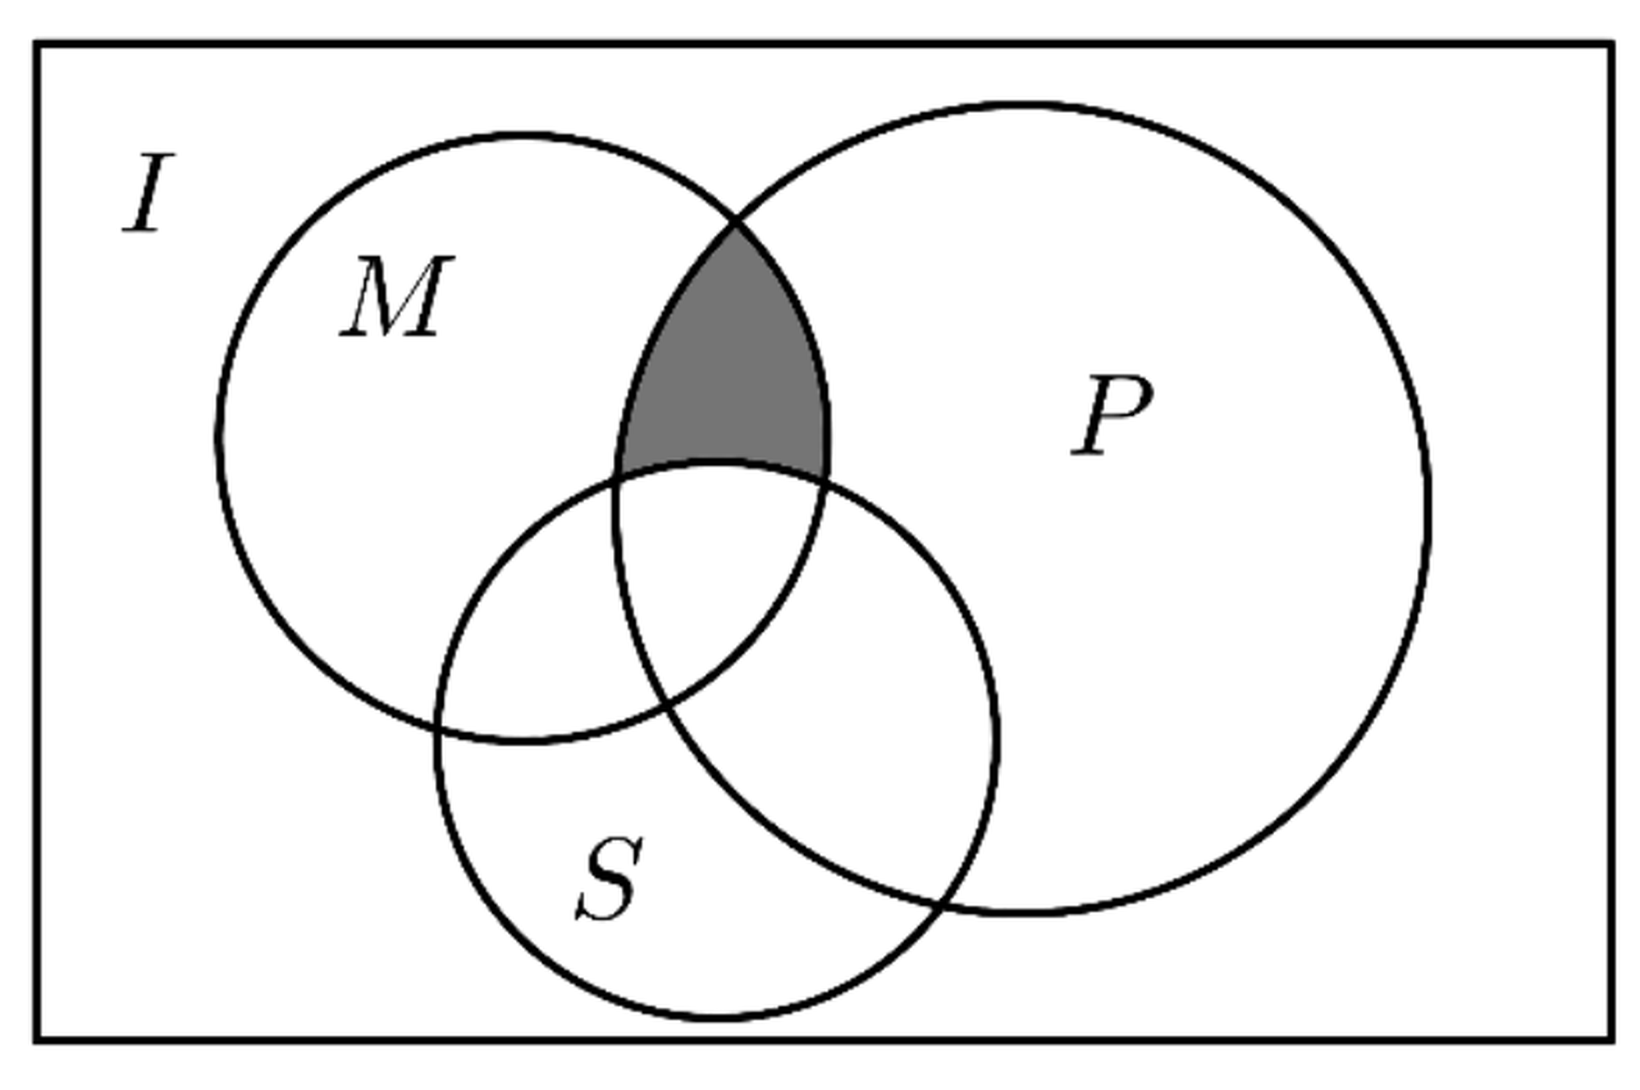
\includegraphics[width=0.42\textwidth]{figures/gao120_q15.png}
\end{center}

\keepwithprev
A. $(M\cap P)\cap S$\qquad\quad B. $(M\cap P)\cap\complement_{I}S$\qquad\quad C. $(M\cup P)\cap S$\qquad\quad D. $\complement_{I}(M\cap P)\cap S$

\ifanswer
\solbegin
\step{由已知中的 $Venn$ 图得阴影部分的元素属于 $M$，属于 $P$，但不属于 $S$，}
\step{所以阴影部分表示的集合为 $(M\cap P)\cap\complement_{I}S$，故选 $B$.}
\solend
\fi

\item 设集合 $P_1=\{x\mid x^2+ax+1>0\}$，$P_2=\{x\mid x^2+ax+2>0\}$，$Q_1=\{x\mid x^2+x+b>0\}$，$Q_2=\{x\mid x^2+2x+b>0\}$，其中 $a$、$b\in\R$，对于下列两个命题：①存在 $a$，$P_1$ 不是 $P_2$ 的子集；②存在 $b$ 使得 $Q_1$ 是 $Q_2$ 的子集. 下列说法正确的是\mbox{（\quad）}

\keepwithprev
A. ①是真命题，②是假命题\qquad\qquad B. ①是假命题，②是真命题

C. ①②都是真命题\qquad\qquad\qquad D. ①②都是假命题

\ifanswer
\solbegin
\step{对于集合 $P_1=\{x\mid x^2+ax+1>0\}$，$P_2=\{x\mid x^2+ax+2>0\}$，}
\step{得当 $m\in P_1$ 时，即 $m^2+am+1>0$，得 $m^2+am+2>0$，}
\step{即有 $m\in P_2$，得对任意 $a$，$P_1$ 是 $P_2$ 的子集，故①错误；}
\step{对于集合 $Q_1=\{x\mid x^2+x+b>0\}$，$Q_2=\{x\mid x^2+2x+b>0\}$，}
\step{当 $b=6$ 时，$Q_1=\{x\mid x^2+x+6>0\}=\R$，$Q_2=\{x\mid x^2+2x+6>0\}=\R$，}
\step{得 $Q_1$ 是 $Q_2$ 的子集，所以存在 $b$，使得 $Q_1$ 是 $Q_2$ 的子集，故②正确；}
\step{故选 $B$.}
\solend
\fi

\end{enumerate}

\bigsec{三、解答题}

\begin{enumerate}
\setcounter{enumi}{16}

\item (1) 已知 $x$、$y$ 都是实数，比较 $x^2+y^2$ 与 $4x-2y-5$ 的大小.

(2) 求解不等式组 $\begin{cases}x^2-4x+3\geqslant0\\\dfrac{x+3}{2x-1}\geqslant2\end{cases}$.

\ifanswer
\solbegin
\step{(1) $(x^2+y^2)-(4x-2y-5)=x^2-4x+y^2+2y+5=(x-2)^2+(y+1)^2\geqslant0$，}
\step{当 $x=2$，$y=-1$ 时，$x^2+y^2=4x-2y-5$.}
\step{当 $x\neq2$ 或 $y\neq-1$ 时，$x^2+y^2>4x-2y-5$.}
\step{(2) 由 $x^2-4x+3\geqslant0$ 得 $(x-1)(x-3)\geqslant0$，所以 $x\leqslant1$ 或 $x\geqslant3$；}
\step{由 $\dfrac{x+3}{2x-1}\geqslant2$，得 $\dfrac{x+3}{2x-1}-2=\dfrac{-3x+5}{2x-1}\geqslant0$，即 $\dfrac{3x-5}{2x-1}\leqslant0$，}
\step{所以 $\begin{cases}(3x-5)(2x-1)\leqslant0\\2x-1\neq0\end{cases}$，解得 $\dfrac12<x\leqslant\dfrac53$，}
\step{所以不等式组的解集是 $\left\{x\,\middle\vert\,\dfrac12<x\leqslant1\right\}$.}
\solend
\fi

\item 已知 $x_1$,$x_2$ 是一元二次方程 $4kx^2-4kx+k+1=0$ 的两个实数根.

(1) 是否存在实数 $k$，$(2x_1-x_2)(x_1-2x_2)=-\dfrac32$ 成立？若存在，求出 $k$ 的值；若不存在，请说明理由.

(2) 求使 $\dfrac{x_1}{x_2}+\dfrac{x_2}{x_1}-2$ 的值为整数的实数 $k$ 的整数值.

\ifanswer
\solbegin
\step{(1) 因为 $x_1$,$x_2$ 是一元二次方程 $4kx^2-4kx+k+1=0$ 的两个实数根，}
\step{所以 $\begin{cases}k\neq0\\16k^2-16k(k+1)\geqslant0\end{cases}$，所以 $k<0$，}
\step{由根与系数的关系得 $x_1+x_2=1$，$x_1x_2=\dfrac{k+1}{4k}$，}
\step{所以 $(2x_1-x_2)(x_1-2x_2)=2(x_1+x_2)^2-9x_1x_2=2-9\times\dfrac{k+1}{4k}=-\dfrac32$，}
\step{解得 $k=\dfrac95$，而 $k<0$，故不存在实数 $k$ 使得 $(2x_1-x_2)(x_1-2x_2)=-\dfrac32$ 成立.}
\step{(2) 由根与系数的关系得 $\dfrac{x_1}{x_2}+\dfrac{x_2}{x_1}-2=\dfrac{(x_1+x_2)^2}{x_1x_2}-4=-\dfrac4{k+1}$，}
\step{因为 $-\dfrac4{k+1}$ 的值为整数，而 $k$ 为整数，所以 $k+1$ 只能取 $\pm1$、$\pm2$、$\pm4$，}
\step{又 $k<0$，所以整数 $k$ 的值为 $-2$ 或 $-3$ 或 $-5$.}
\solend
\fi

\item 2026 年，某市低空经济蓬勃发展，一家物流企业开通“无人机即时配送”服务，并设立配送站. 经市场调研，该站每日配送单量 $y$（单位：单）与每单配送费 $x$（单位：元）满足关系式 $y=4800-200x$（其中 $4<x<24$）. 已知配送站每日的固定成本为 $19200$ 元，每完成一单配送，需支付电费、耗材费、设备保养费等可变成本，每单可变成本为 $4$ 元.

(1) 若要保证配送站每日利润 $W$（单位：元）不为负数，求每单配送费 $x$ 的取值范围；（每日利润 $=$ 每日配送总收入 $-$ 每日可变总成本 $-$ 每日固定成本）

(2) 为提升运力，该站购进一批新型无人机，购机费用为 $32$ 万元. 投入使用后，这批无人机使用 $t(t>0)$ 年的累计维保总费用为 $(2t^2+8t)$ 万元. 请问：这批无人机使用多少年后更新，可以使年平均总费用最低？请求出最低年平均总费用.（年平均总费用 $=$（购机费用 $+$ 维保总费用）$\div$ 使用年数）

\ifanswer
\solbegin
\step{(1) $W=xy-4y-19200=x(4800-200x)-4(4800-200x)-19200$}
\step{$=-200x^2+5600x-38400(4<x<24)$，}
\step{令 $W=-200x^2+5600x-38400\geqslant0$，即 $x^2-28x+192\leqslant0$，}
\step{解得 $12\leqslant x\leqslant16$，因此，要保证配送站每日利润 $W$ 不为负数，}
\step{每单配送费 $x$ 的取值范围为 $[12,16]$；}
\step{(2) 由题意，年平均总费用为 $N=\dfrac{2t^2+8t+32}{t}=2t+\dfrac{32}{t}+8$}
\step{$\geqslant2\sqrt{2t\cdot\dfrac{32}{t}}+8=16+8=24$，当且仅当 $2t=\dfrac{32}{t}$，即 $t=4$ 时取等号，}
\step{则这批无人机使用 $4$ 年后更新，可以使年平均总费用最低，}
\step{最低年平均总费用为 $24$ 万元.}
\solend
\fi

\item 已知 $A,B$，定义集合 $M_{(A,B)}=\{x\mid A<B\}$.

(1) 设 $A=\lvert x-4\rvert$,$B=2x$，求 $M_{(A,B)}$；

(2) 设 $A=ax^2+2ax-4$,$B=2x(x+2)$，当 $M_{(A,B)}=\R$ 时，求 $a$ 的取值范围；

(3) 设 $A=\lvert 2x-b\rvert$,$B=\dfrac{x+4b}{x-1}$,$C=2$，若 $M_{(A,C)}\cap M_{(B,C)}\neq\varnothing$，求 $b$ 的取值范围.

\ifanswer
\solbegin
\step{(1) 由定义，$x\in M_{(A,B)}$ 等价于 $\lvert x-4\rvert<2x$，}
\step{原不等式等价于 $-2x<x-4<2x$，即同时满足 $3x>4$ 与 $x>-4$，}
\step{解得 $x>\dfrac43$，所以 $M_{(A,B)}=\left(\dfrac43,+\infty\right)$.}
\step{(2) 由 $M_{(A,B)}=\R$，得 $ax^2+2ax-4<2x(x+2)$ 对任意 $x\in\R$ 恒成立，}
\step{得 $(a-2)(x+1)^2-a-2<0$.}
\step{当 $a>2$ 时，随着 $(x+1)^2$ 增大，左边可取正值，不符合题意；}
\step{当 $a=2$ 时，左边恒等于 $-4$，符合题意；}
\step{当 $a<2$ 时，左边在 $x=-1$ 处取得最大值 $-a-2$，}
\step{故恒成立的充要条件为 $-a-2<0$，即 $a>-2$；}
\step{综上，$a\in(-2,2]$.}
\step{(3) 由 $\lvert 2x-b\rvert<2$，得 $M_{(A,C)}=\left(\dfrac b2-1,\dfrac b2+1\right)$，记为 $I$.}
\step{由 $\dfrac{x+4b}{x-1}<2$，得 $\dfrac{x-(4b+2)}{x-1}>0$，其中 $x\neq1$.}
\step{①当 $b<-\dfrac14$ 时，$4b+2<1$，故 $M_{(B,C)}=(-\infty,4b+2)\cup(1,+\infty)$.}
\step{此时 $\dfrac b2+1<1$，所以 $I$ 与 $(1,+\infty)$ 没有公共元素.}
\step{两集合交集非空等价于 $\dfrac b2-1<4b+2$，解得 $b>-\dfrac67$.}
\step{因而本种情况得到 $-\dfrac67<b<-\dfrac14$.}
\step{②当 $b=-\dfrac14$ 时，$\dfrac{x+4b}{x-1}=1$，其中 $x\neq1$，故 $M_{(B,C)}=\{x\mid x\neq1\}$.}
\step{此时 $I=\left(-\dfrac98,\dfrac78\right)$，两集合交集非空.}
\step{③当 $b>-\dfrac14$ 时，$4b+2>1$，故 $M_{(B,C)}=(-\infty,1)\cup(4b+2,+\infty)$.}
\step{此时 $4b+2-\left(\dfrac b2+1\right)=\dfrac{7b}{2}+1>\dfrac18>0$，}
\step{所以 $I$ 与 $(4b+2,+\infty)$ 没有公共元素.}
\step{两集合交集非空等价于 $\dfrac b2-1<1$，解得 $b<4$.}
\step{因而本种情况得到 $-\dfrac14<b<4$.}
\step{综上，$b\in\left(-\dfrac67,4\right)$.}
\solend
\fi

\item 破晓同学阅读课外书籍时，发现笛卡尔积是代数和图论中一个很重要的课题. 对于非空数集 $A,B$，定义 $A\otimes B=\{(x,y)\mid x\in A$ 且 $y\in B\}$，将 $A\otimes B$ 称为“$A$ 与 $B$ 的笛卡尔积”.

(1) 若 $A=\{-1,0,1\}$,$B=\{-1,1\}$，求 $A\otimes B$ 和 $B\otimes A$；

(2) 试证明：“$A_1\otimes A_2=A_2\otimes A_1$”是“$A_1=A_2$”的充要条件；

(3) 若集合 $H$ 是有限集，将集合 $H$ 的元素个数记为 $\lvert H\rvert$. 已知 $\lvert A_1\otimes A_2\rvert=m^3(m\in\N^*)$，且存在实数 $a$ 满足 $\sqrt{\dfrac{\lvert A_1\otimes A_1\rvert+\lvert A_2\otimes A_2\rvert}{\lvert A_2\otimes A_1\rvert}}\geqslant a$ 对任意 $m\in\N^*$ 恒成立. 求 $a$ 的取值范围，并指明当 $a$ 取到最值时 $\lvert A_1\rvert$ 和 $\lvert A_2\rvert$ 满足的关系式及 $m$ 应满足的条件.

\ifanswer
\solbegin
\step{(1) 由题意得 $A\otimes B=\{(-1,-1),(-1,1),(0,-1),(0,1),(1,-1),(1,1)\}$，}
\step{$B\otimes A=\{(-1,-1),(-1,0),(-1,1),(1,-1),(1,0),(1,1)\}$；}
\step{(2) 若 $A_1=A_2$，设 $A_1=A_2=A$，}
\step{由定义得 $A_1\otimes A_2=\{(a,b)\mid a\in A$ 且 $b\in A\}=A_2\otimes A_1$，}
\step{所以“$A_1\otimes A_2=A_2\otimes A_1$”是“$A_1=A_2$”的必要条件；}
\step{若 $A_1\otimes A_2=A_2\otimes A_1$，对任意 $(a,b)\in A_1\otimes A_2$，均有 $(a,b)\in A_2\otimes A_1$，}
\step{即对任意 $a\in A_1,b\in A_2$，均有 $a\in A_2,b\in A_1$，}
\step{由任意性得 $A_1\subseteq A_2,A_2\subseteq A_1$，则 $A_1=A_2$，}
\step{所以“$A_1\otimes A_2=A_2\otimes A_1$”是“$A_1=A_2$”的充分条件；}
\step{综上所述，“$A_1\otimes A_2=A_2\otimes A_1$”是“$A_1=A_2$”的充要条件.}
\step{(3) 设 $\lvert A_1\rvert=c$,$\lvert A_2\rvert=d$,$c,d\in\N^*$，}
\step{则 $\lvert A_1\otimes A_2\rvert=\lvert A_2\otimes A_1\rvert=cd=m^3$,$\lvert A_1\otimes A_1\rvert=c^2$,$\lvert A_2\otimes A_2\rvert=d^2$，}
\step{得 $\sqrt{\dfrac{\lvert A_1\otimes A_1\rvert+\lvert A_2\otimes A_2\rvert}{\lvert A_2\otimes A_1\rvert}}=\sqrt{\dfrac{c^2+d^2}{cd}}=\sqrt{\dfrac cd+\dfrac dc}\geqslant\sqrt{2\sqrt{\dfrac cd\cdot\dfrac dc}}=\sqrt2$，}
\step{当且仅当 $\dfrac cd=\dfrac dc$，即 $c=d$ 时取等号，所以实数 $a$ 的取值范围是 $(-\infty,\sqrt2]$.}
\step{若 $a$ 取到最大值，则 $c=d$，即 $\lvert A_1\rvert=\lvert A_2\rvert$，得 $c^2=m^3$，}
\step{即 $c=\sqrt{m^3}=(\sqrt m)^3\in\N^*$，所以 $m=k^2,k\in\N^*$.}
\solend
\fi

\end{enumerate}

\end{document}
"
%
% 原始材料：微信公众号“魔都数学加油站”文章，作者破晓，2026-11-08 21:35 发布；
% 连载“27学年高一120”，原文标题“27学年高一120——2026-2027年上海市松江二中高一上10月月考”；
% 原文链接：https://mp.weixin.qq.com/s/hgDkaZX9M_IKhmr7CjQc1A。
% 正文为 10 张 PNG 页（第 8、10 页 2560×3620，其余 4762×6735），
% 题目下印有【解析】或【答案】，为讲评版。
% 题目、解析均据原图转录；卷面红色水印及公众号页脚未录入。
% 全卷 1 张插图：第 15 题的三集合 Venn 图（原卷印在题干右侧，本稿移至题干之后，
% 取原卷截图 2× LANCZOS 放大，见 figures/gao120_q15.png）。
%
% 卷首标题：原卷印作“2026-2027 年松江二中高一上 10 月月考”（公众号标题中的“上海市”
% 卷面标题行没有，本稿照卷面），年份区间按全稿惯例排 en dash；原卷未印副标题，本稿按题目内容
% 标为“集合与常用逻辑用语、不等式”（与 110／111／113／116／118 同）。
%
% 与原卷的排版差异：
%   ① 原文从第 3 题起，填空题编号为 3—12、选择题为 13—16、解答题为 17—21，本稿保留原题号；
%   ② 原卷每题下直接印【解析】／【答案】，本稿按全稿惯例置于答案版；第 3 题只印【答案】、
%      第 13、14 题把答案印在题干括号内且无【解析】，均另提 \ans{}；其余选择题答案在
%      解析末句“故选 …”，括号内留空；
%   ③ 原卷未印副标题，本稿按“知识模块”口径补出；
%   ④ 原卷填空横线按全稿惯例排为 \blankline[4.4em]；选择题括号排 \mbox{（\quad）}、
%      选项段前按惯例加 \keepwithprev；解答题不留作答区（原卷为讲评版，与 109—119 同）；
%   ⑤ 原卷数集排斜体 $R$、$N^*$，按全稿惯例改 \R、\N^*；绝对值排 \lvert…\rvert，
%      集合描述竖线排 \mid；补集记号照原卷排 \complement_I。
%
% 判别式字形：第 9 题解析作 $\triangle$（等边、扁），照录 \triangle。
%
% 子集符号：第 4 题题干与解析的 $A\subseteq B$、第 21 题 (2) 的 $A_1\subseteq A_2$ 印有下划线，
%   照录 \subseteq。
%
% 原卷存疑照录：第 12 题题干 $S=\{82,83,84,85,86,87,89\}$ 跳过 $88$ 只列 7 个数，
%   与其“8 种不同的值”自洽（不含 $88$），照录；第 19 题 (1) 的 $W$ 表达式
%   $x(4800-200x)-4(4800-200x)-19200$ 与最后结果 $[12,16]$ 一致。
%
% 行数核对：逐题数 \step 条数，合计 115 条（Q3：0；Q4：4；Q5：2；Q6：5；Q7：4；
% Q8：2；Q9：5；Q10：3；Q11：6；Q12：11；Q13：0；Q14：0；Q15：2；Q16：7；
% Q17：7；Q18：8；Q19：9；Q20：24；Q21：16），与原卷印刷行逐题相等
% （cases 块作一个印刷行计）。第 3 题只印【答案】、第 13、14 题括号内印答案且无解析，
% 均提 \ans{}，不计入 \step 账。
%
\documentclass[a4paper,11pt]{article}
\usepackage{common}

\begin{document}

\examtitlest[3]{2026--2027 年松江二中高一上 10 月月考}{集合与常用逻辑用语、不等式}

\bigsec{一、填空题}

\begin{enumerate}
\setcounter{enumi}{2}

\item 集合 $A=\{(x,y)\mid x+y=8\}$,$B=\{(x,y)\mid xy=12\}$，求 $A\cap B=$\blankline[4.4em].

\ifanswer
\ans{$\{(2,6),(6,2)\}$}
\fi

\item 设集合 $A=\{0,-a\}$,$B=\{1,a-2,2a-2\}$，若 $A\subseteq B$，则 $a=$\blankline[4.4em].

\ifanswer
\solbegin
\step{因为 $A\subseteq B$，}
\step{若 $a-2=0$，解得 $a=2$，此时 $A=\{0,-2\}$,$B=\{1,0,2\}$，不符合题意；}
\step{若 $2a-2=0$，解得 $a=1$，此时 $A=\{0,-1\}$,$B=\{1,-1,0\}$，符合题意；}
\step{综上所述，$a=1$.}
\solend
\fi

\item 设 $\alpha:0<x<a(a>0)$,$\beta:x<8-3a$，若 $\alpha$ 是 $\beta$ 的充分条件，则实数 $a$ 的取值范围是\blankline[4.4em].

\ifanswer
\solbegin
\step{由 $\alpha$ 是 $\beta$ 的充分条件得，$x\in(0,a)\Rightarrow x\in(-\infty,8-3a)$，}
\step{所以 $0<a\leqslant8-3a$，解得 $0<a\leqslant2$.}
\solend
\fi

\item 关于 $x$ 的不等式 $ax-b>0$ 的解集为 $(-\infty,1)$，则不等式 $\dfrac{x-2}{ax+b}<0$ 的解集为\blankline[4.4em].

\ifanswer
\solbegin
\step{因为关于 $x$ 的不等式 $ax-b>0$ 的解集为 $(-\infty,1)$，}
\step{所以 $a<0$ 且 $\dfrac ba=1$，则 $b=a$，}
\step{所以不等式 $\dfrac{x-2}{ax+b}<0$，即 $\dfrac{x-2}{ax+a}<0$，即 $\dfrac{x-2}{x+1}>0$，}
\step{等价于 $(x+1)(x-2)>0$，解得 $x>2$ 或 $x<-1$，}
\step{即解集为 $(-\infty,-1)\cup(2,+\infty)$.}
\solend
\fi

\item 若正实数 $x$、$y$ 满足 $2x+y+8xy=2$，则 $xy$ 的最大值为\blankline[4.4em].

\ifanswer
\solbegin
\step{因为正实数 $x$、$y$ 满足 $2x+y+8xy=2$，}
\step{所以 $2-8xy=2x+y\geqslant2\sqrt{2xy}$，}
\step{当且仅当 $y=2x$，即 $x=\dfrac14$，$y=\dfrac12$ 时取等号，解得 $0<xy\leqslant\dfrac18$，}
\step{故 $xy$ 的最大值为 $\dfrac18$.}
\solend
\fi

\item 已知 $1<a<3$，$-5<b<-2$，则 $\dfrac ab$ 的取值范围是\blankline[4.4em].

\ifanswer
\solbegin
\step{因为 $-5<b<-2$，所以 $2<-b<5$，$\dfrac15<-\dfrac1b<\dfrac12$，又 $1<a<3$，}
\step{得 $\dfrac15<-\dfrac ab<\dfrac32$，则 $-\dfrac32<\dfrac ab<-\dfrac15$，故 $\dfrac ab$ 的取值范围是 $\left(-\dfrac32,-\dfrac15\right)$.}
\solend
\fi

\item 若关于 $x$、$y$ 的方程组 $\begin{cases}y-kx-2=0\\y^2-4x-2y+1=0\end{cases}$ 的解集中只有一个元素，则实数 $k$ 的值为\blankline[4.4em].

\ifanswer
\solbegin
\step{由 $\begin{cases}y-kx-2=0\\y^2-4x-2y+1=0\end{cases}$ 消去 $y$ 整理得 $k^2x^2+(2k-4)x+1=0$.}
\step{当 $k\neq0$ 时，则 $\triangle=(2k-4)^2-4k^2=0$，解得 $k=1$，}
\step{此时方程组的解为 $\begin{cases}x=1\\y=3\end{cases}$，符合题意；}
\step{当 $k=0$ 时，解得 $x=\dfrac14$，此时方程组的解为 $\begin{cases}x=\dfrac14\\y=2\end{cases}$，符合题意；}
\step{综上，$k=0$ 或 $k=1$.}
\solend
\fi

\item 若集合 $A=\{0,1\}$，$B=\{x\mid x^2-mx-m>0,x\in\R\}$，且 $A\cap B=\{1\}$，则实数 $m$ 的取值范围为\blankline[4.4em].

\ifanswer
\solbegin
\step{因为集合 $A=\{0,1\}$，$B=\{x\mid x^2-mx-m>0,x\in\R\}$，且 $A\cap B=\{1\}$，}
\step{则 $1\in B$ 且 $0\notin B$，所以 $\begin{cases}1-m-m>0\\-m\leqslant0\end{cases}$，解得 $0\leqslant m<\dfrac12$，}
\step{所以实数 $m$ 的取值范围是 $\left[0,\dfrac12\right)$.}
\solend
\fi

\item 从集合 $U=\{a,b,c,d\}$ 的子集中选出两个不同的子集，需同时满足以下两个条件：(1) $a$、$b$ 都至少属于其中一个集合；(2) 对选出的两个子集，其中一个集合为另一个的子集，那么共有\blankline[4.4em]种不同的选法.

\ifanswer
\solbegin
\step{不妨设元素少的为 $A$，元素多的为 $B$，则 $B$ 必包含有 $a$、$b$；$A$ 为 $B$ 的真子集，}
\step{若 $B=\{a,b\}$，$A$ 为 $B$ 的真子集，共 $2^2-1=3$ 种，}
\step{若 $B=\{a,b,c\}$，$A$ 为 $B$ 的真子集，共 $2^3-1=7$ 种，}
\step{若 $B=\{a,b,d\}$，$A$ 为 $B$ 的真子集，共 $2^3-1=7$ 种，}
\step{若 $B=\{a,b,c,d\}$，$A$ 为 $B$ 的真子集，共 $2^4-1=15$ 种，}
\step{共有 $3+7+7+15=32$ 种.}
\solend
\fi

\item 已知 $a_1$、$a_2$、$\cdots$、$a_8$ 是 $8$ 个正整数，记 $S=\{a_{i_1}+a_{i_2}+\cdots+a_{i_7}\mid 1\leqslant i_1<i_2<\cdots<i_7\leqslant8\}$，其中 $i_1$、$i_2$、$\cdots$、$i_7\in\N^*$，若 $S=\{82,83,84,85,86,87,89\}$，则这 $8$ 个正整数中的最大数与最小数的积为\blankline[4.4em].

\ifanswer
\solbegin
\step{由题意得从 $8$ 个数中任取 $7$ 个数的和共有 $C_8^7=8$ 种不同的值，}
\step{但是 $82$，$83$，$84$，$85$，$86$，$87$，$89$ 只有 $7$ 个数，}
\step{得必有两种 $7$ 个数的和相等，设这个和为 $t(82\leqslant t\leqslant89)$，}
\step{令 $T=\sum\limits_{i=1}^{8}a_i$，那么，任取 $7$ 个数的和就等于 $T-a_i$，$i=1,2,\cdots,8$，}
\step{这 $8$ 个取值和的集合为 $S$，$S=\{T-a_1,T-a_2,\cdots,T-a_8\}$，}
\step{则 $\sum\limits_{i=1}^{8}(T-a_i)=8T-T=7T=82+83+84+85+86+87+89+t=596+t$.}
\step{因为 $T$ 为整数，所以 $596+t$ 是 $7$ 的倍数，}
\step{由 $596=7\times85+1$ 得 $1+t$ 是 $7$ 的倍数，}
\step{再因为 $82\leqslant t\leqslant89$，所以 $t=83$，得 $T=97$.}
\step{因此 $a_1$、$a_2$、$\cdots$、$a_8$ 中最大数为 $97-82=15$，最小数为 $97-89=8$，}
\step{因此，它们的积为 $120$.}
\solend
\fi

\end{enumerate}

\bigsec{二、选择题}

\begin{enumerate}
\setcounter{enumi}{12}

\item 已知 $a>b>0$，$c\in\R$，则下列不等式不一定成立的是\mbox{（\quad）}% 原卷把答案“$B$”印在题干括号内、无【解析】

\keepwithprev
A. $a-c>b-c$\qquad\quad B. $ac>bc$\qquad\quad C. $\dfrac1a<\dfrac1b$\qquad\quad D. $\dfrac{a+b}{2}>\sqrt{ab}$

\ifanswer
\ans{$B$}
\fi

\item 命题“对任意的 $x\in\R,x^3-x^2+1\leqslant0$”的否定是\mbox{（\quad）}% 原卷把答案“$C$”印在题干括号内、无【解析】

\keepwithprev
A. 不存在 $x\in\R,x^3-x^2+1\leqslant0$\qquad B. 存在 $x\in\R,x^3-x^2+1\leqslant0$

C. 存在 $x\in\R,x^3-x^2+1>0$\qquad\quad D. 对任意的 $x\in\R,x^3-x^2+1>0$

\ifanswer
\ans{$C$}
\fi

% 第 15 题是“题干 + 图 + 选项”约 6.5cm 的一整块，\keepwithprev 只挡得住“图—选项”，
% 挡不住夹在中间的图——实测断点落在题干之后（切页审计 A 类）。故照 高一30／高一26 成例
% 在题前先量一次页高，不够就把整块一起挪到次页。
\needvspace{7cm}
\item 如图，$I$ 是全集，$M$、$P$、$S$ 是 $I$ 的三个子集，则阴影部分所表示的集合是\mbox{（\quad）}

\begin{center}
% 图取原卷截图（第 4 页题干右侧）、2× LANCZOS 放大，本稿移至题干之后
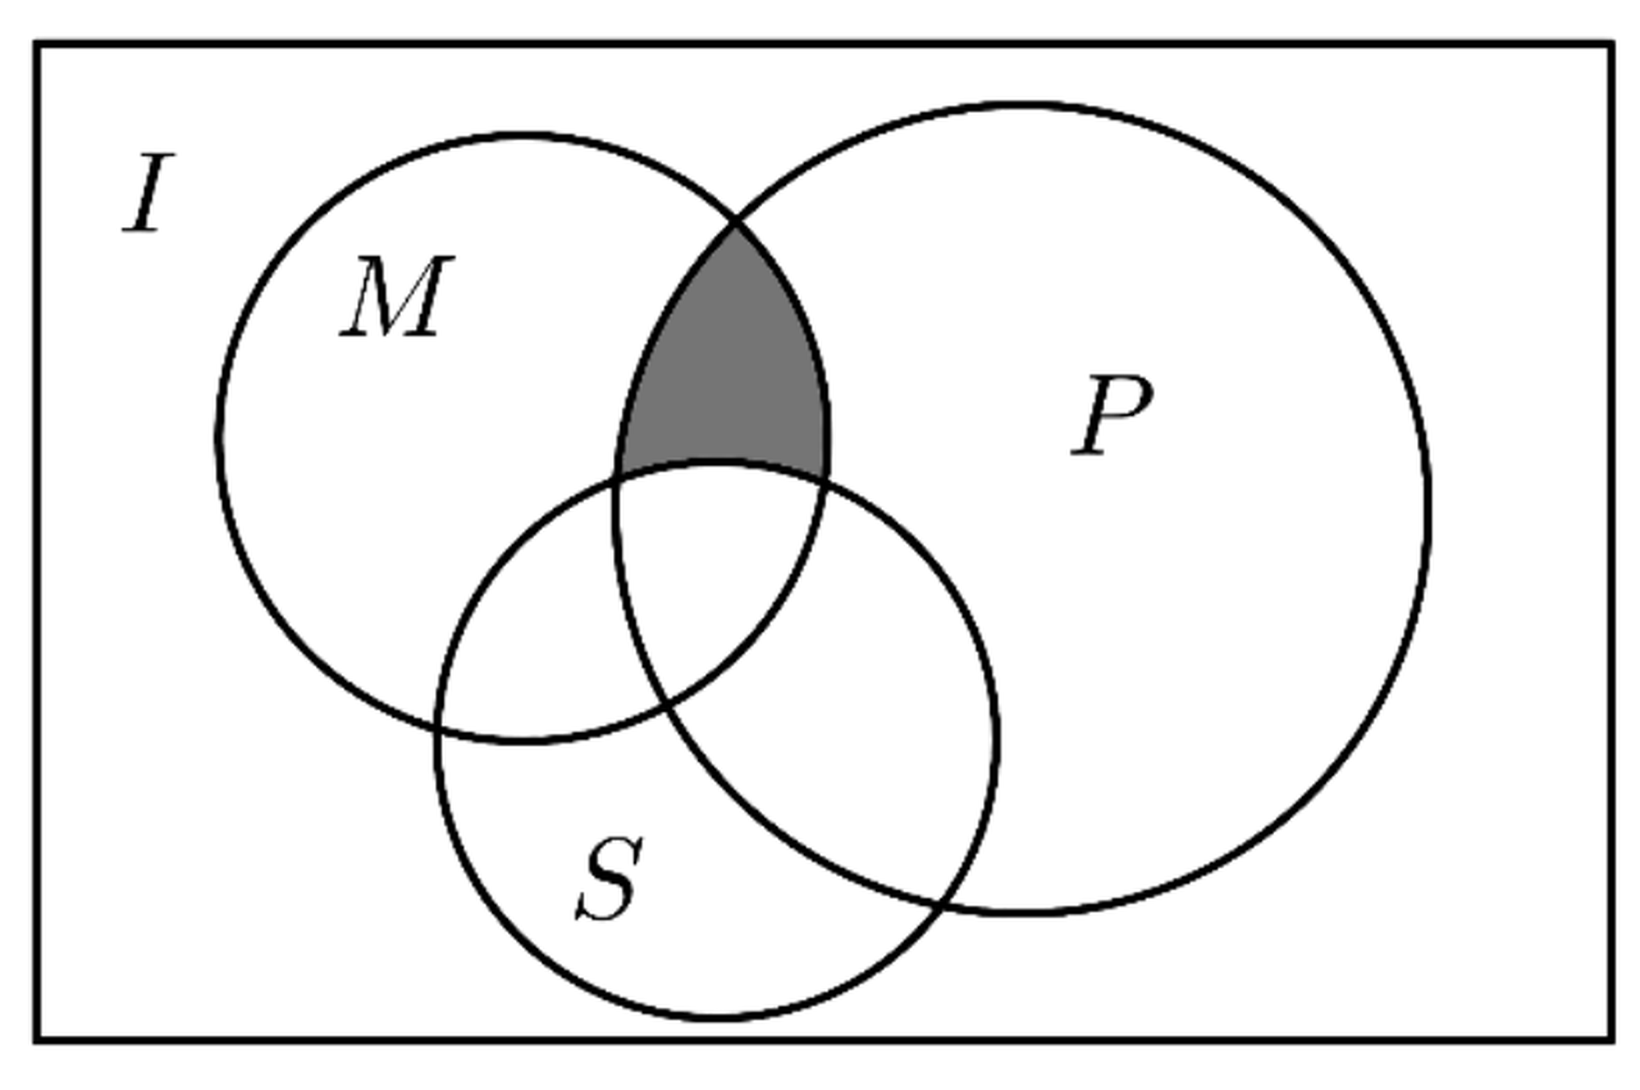
\includegraphics[width=0.42\textwidth]{figures/gao120_q15.png}
\end{center}

\keepwithprev
A. $(M\cap P)\cap S$\qquad\quad B. $(M\cap P)\cap\complement_{I}S$\qquad\quad C. $(M\cup P)\cap S$\qquad\quad D. $\complement_{I}(M\cap P)\cap S$

\ifanswer
\solbegin
\step{由已知中的 $Venn$ 图得阴影部分的元素属于 $M$，属于 $P$，但不属于 $S$，}
\step{所以阴影部分表示的集合为 $(M\cap P)\cap\complement_{I}S$，故选 $B$.}
\solend
\fi

\item 设集合 $P_1=\{x\mid x^2+ax+1>0\}$，$P_2=\{x\mid x^2+ax+2>0\}$，$Q_1=\{x\mid x^2+x+b>0\}$，$Q_2=\{x\mid x^2+2x+b>0\}$，其中 $a$、$b\in\R$，对于下列两个命题：①存在 $a$，$P_1$ 不是 $P_2$ 的子集；②存在 $b$ 使得 $Q_1$ 是 $Q_2$ 的子集. 下列说法正确的是\mbox{（\quad）}

\keepwithprev
A. ①是真命题，②是假命题\qquad\qquad B. ①是假命题，②是真命题

C. ①②都是真命题\qquad\qquad\qquad D. ①②都是假命题

\ifanswer
\solbegin
\step{对于集合 $P_1=\{x\mid x^2+ax+1>0\}$，$P_2=\{x\mid x^2+ax+2>0\}$，}
\step{得当 $m\in P_1$ 时，即 $m^2+am+1>0$，得 $m^2+am+2>0$，}
\step{即有 $m\in P_2$，得对任意 $a$，$P_1$ 是 $P_2$ 的子集，故①错误；}
\step{对于集合 $Q_1=\{x\mid x^2+x+b>0\}$，$Q_2=\{x\mid x^2+2x+b>0\}$，}
\step{当 $b=6$ 时，$Q_1=\{x\mid x^2+x+6>0\}=\R$，$Q_2=\{x\mid x^2+2x+6>0\}=\R$，}
\step{得 $Q_1$ 是 $Q_2$ 的子集，所以存在 $b$，使得 $Q_1$ 是 $Q_2$ 的子集，故②正确；}
\step{故选 $B$.}
\solend
\fi

\end{enumerate}

\bigsec{三、解答题}

\begin{enumerate}
\setcounter{enumi}{16}

\item (1) 已知 $x$、$y$ 都是实数，比较 $x^2+y^2$ 与 $4x-2y-5$ 的大小.

(2) 求解不等式组 $\begin{cases}x^2-4x+3\geqslant0\\\dfrac{x+3}{2x-1}\geqslant2\end{cases}$.

\ifanswer
\solbegin
\step{(1) $(x^2+y^2)-(4x-2y-5)=x^2-4x+y^2+2y+5=(x-2)^2+(y+1)^2\geqslant0$，}
\step{当 $x=2$，$y=-1$ 时，$x^2+y^2=4x-2y-5$.}
\step{当 $x\neq2$ 或 $y\neq-1$ 时，$x^2+y^2>4x-2y-5$.}
\step{(2) 由 $x^2-4x+3\geqslant0$ 得 $(x-1)(x-3)\geqslant0$，所以 $x\leqslant1$ 或 $x\geqslant3$；}
\step{由 $\dfrac{x+3}{2x-1}\geqslant2$，得 $\dfrac{x+3}{2x-1}-2=\dfrac{-3x+5}{2x-1}\geqslant0$，即 $\dfrac{3x-5}{2x-1}\leqslant0$，}
\step{所以 $\begin{cases}(3x-5)(2x-1)\leqslant0\\2x-1\neq0\end{cases}$，解得 $\dfrac12<x\leqslant\dfrac53$，}
\step{所以不等式组的解集是 $\left\{x\,\middle\vert\,\dfrac12<x\leqslant1\right\}$.}
\solend
\fi

\item 已知 $x_1$,$x_2$ 是一元二次方程 $4kx^2-4kx+k+1=0$ 的两个实数根.

(1) 是否存在实数 $k$，$(2x_1-x_2)(x_1-2x_2)=-\dfrac32$ 成立？若存在，求出 $k$ 的值；若不存在，请说明理由.

(2) 求使 $\dfrac{x_1}{x_2}+\dfrac{x_2}{x_1}-2$ 的值为整数的实数 $k$ 的整数值.

\ifanswer
\solbegin
\step{(1) 因为 $x_1$,$x_2$ 是一元二次方程 $4kx^2-4kx+k+1=0$ 的两个实数根，}
\step{所以 $\begin{cases}k\neq0\\16k^2-16k(k+1)\geqslant0\end{cases}$，所以 $k<0$，}
\step{由根与系数的关系得 $x_1+x_2=1$，$x_1x_2=\dfrac{k+1}{4k}$，}
\step{所以 $(2x_1-x_2)(x_1-2x_2)=2(x_1+x_2)^2-9x_1x_2=2-9\times\dfrac{k+1}{4k}=-\dfrac32$，}
\step{解得 $k=\dfrac95$，而 $k<0$，故不存在实数 $k$ 使得 $(2x_1-x_2)(x_1-2x_2)=-\dfrac32$ 成立.}
\step{(2) 由根与系数的关系得 $\dfrac{x_1}{x_2}+\dfrac{x_2}{x_1}-2=\dfrac{(x_1+x_2)^2}{x_1x_2}-4=-\dfrac4{k+1}$，}
\step{因为 $-\dfrac4{k+1}$ 的值为整数，而 $k$ 为整数，所以 $k+1$ 只能取 $\pm1$、$\pm2$、$\pm4$，}
\step{又 $k<0$，所以整数 $k$ 的值为 $-2$ 或 $-3$ 或 $-5$.}
\solend
\fi

\item 2026 年，某市低空经济蓬勃发展，一家物流企业开通“无人机即时配送”服务，并设立配送站. 经市场调研，该站每日配送单量 $y$（单位：单）与每单配送费 $x$（单位：元）满足关系式 $y=4800-200x$（其中 $4<x<24$）. 已知配送站每日的固定成本为 $19200$ 元，每完成一单配送，需支付电费、耗材费、设备保养费等可变成本，每单可变成本为 $4$ 元.

(1) 若要保证配送站每日利润 $W$（单位：元）不为负数，求每单配送费 $x$ 的取值范围；（每日利润 $=$ 每日配送总收入 $-$ 每日可变总成本 $-$ 每日固定成本）

(2) 为提升运力，该站购进一批新型无人机，购机费用为 $32$ 万元. 投入使用后，这批无人机使用 $t(t>0)$ 年的累计维保总费用为 $(2t^2+8t)$ 万元. 请问：这批无人机使用多少年后更新，可以使年平均总费用最低？请求出最低年平均总费用.（年平均总费用 $=$（购机费用 $+$ 维保总费用）$\div$ 使用年数）

\ifanswer
\solbegin
\step{(1) $W=xy-4y-19200=x(4800-200x)-4(4800-200x)-19200$}
\step{$=-200x^2+5600x-38400(4<x<24)$，}
\step{令 $W=-200x^2+5600x-38400\geqslant0$，即 $x^2-28x+192\leqslant0$，}
\step{解得 $12\leqslant x\leqslant16$，因此，要保证配送站每日利润 $W$ 不为负数，}
\step{每单配送费 $x$ 的取值范围为 $[12,16]$；}
\step{(2) 由题意，年平均总费用为 $N=\dfrac{2t^2+8t+32}{t}=2t+\dfrac{32}{t}+8$}
\step{$\geqslant2\sqrt{2t\cdot\dfrac{32}{t}}+8=16+8=24$，当且仅当 $2t=\dfrac{32}{t}$，即 $t=4$ 时取等号，}
\step{则这批无人机使用 $4$ 年后更新，可以使年平均总费用最低，}
\step{最低年平均总费用为 $24$ 万元.}
\solend
\fi

\item 已知 $A,B$，定义集合 $M_{(A,B)}=\{x\mid A<B\}$.

(1) 设 $A=\lvert x-4\rvert$,$B=2x$，求 $M_{(A,B)}$；

(2) 设 $A=ax^2+2ax-4$,$B=2x(x+2)$，当 $M_{(A,B)}=\R$ 时，求 $a$ 的取值范围；

(3) 设 $A=\lvert 2x-b\rvert$,$B=\dfrac{x+4b}{x-1}$,$C=2$，若 $M_{(A,C)}\cap M_{(B,C)}\neq\varnothing$，求 $b$ 的取值范围.

\ifanswer
\solbegin
\step{(1) 由定义，$x\in M_{(A,B)}$ 等价于 $\lvert x-4\rvert<2x$，}
\step{原不等式等价于 $-2x<x-4<2x$，即同时满足 $3x>4$ 与 $x>-4$，}
\step{解得 $x>\dfrac43$，所以 $M_{(A,B)}=\left(\dfrac43,+\infty\right)$.}
\step{(2) 由 $M_{(A,B)}=\R$，得 $ax^2+2ax-4<2x(x+2)$ 对任意 $x\in\R$ 恒成立，}
\step{得 $(a-2)(x+1)^2-a-2<0$.}
\step{当 $a>2$ 时，随着 $(x+1)^2$ 增大，左边可取正值，不符合题意；}
\step{当 $a=2$ 时，左边恒等于 $-4$，符合题意；}
\step{当 $a<2$ 时，左边在 $x=-1$ 处取得最大值 $-a-2$，}
\step{故恒成立的充要条件为 $-a-2<0$，即 $a>-2$；}
\step{综上，$a\in(-2,2]$.}
\step{(3) 由 $\lvert 2x-b\rvert<2$，得 $M_{(A,C)}=\left(\dfrac b2-1,\dfrac b2+1\right)$，记为 $I$.}
\step{由 $\dfrac{x+4b}{x-1}<2$，得 $\dfrac{x-(4b+2)}{x-1}>0$，其中 $x\neq1$.}
\step{①当 $b<-\dfrac14$ 时，$4b+2<1$，故 $M_{(B,C)}=(-\infty,4b+2)\cup(1,+\infty)$.}
\step{此时 $\dfrac b2+1<1$，所以 $I$ 与 $(1,+\infty)$ 没有公共元素.}
\step{两集合交集非空等价于 $\dfrac b2-1<4b+2$，解得 $b>-\dfrac67$.}
\step{因而本种情况得到 $-\dfrac67<b<-\dfrac14$.}
\step{②当 $b=-\dfrac14$ 时，$\dfrac{x+4b}{x-1}=1$，其中 $x\neq1$，故 $M_{(B,C)}=\{x\mid x\neq1\}$.}
\step{此时 $I=\left(-\dfrac98,\dfrac78\right)$，两集合交集非空.}
\step{③当 $b>-\dfrac14$ 时，$4b+2>1$，故 $M_{(B,C)}=(-\infty,1)\cup(4b+2,+\infty)$.}
\step{此时 $4b+2-\left(\dfrac b2+1\right)=\dfrac{7b}{2}+1>\dfrac18>0$，}
\step{所以 $I$ 与 $(4b+2,+\infty)$ 没有公共元素.}
\step{两集合交集非空等价于 $\dfrac b2-1<1$，解得 $b<4$.}
\step{因而本种情况得到 $-\dfrac14<b<4$.}
\step{综上，$b\in\left(-\dfrac67,4\right)$.}
\solend
\fi

\item 破晓同学阅读课外书籍时，发现笛卡尔积是代数和图论中一个很重要的课题. 对于非空数集 $A,B$，定义 $A\otimes B=\{(x,y)\mid x\in A$ 且 $y\in B\}$，将 $A\otimes B$ 称为“$A$ 与 $B$ 的笛卡尔积”.

(1) 若 $A=\{-1,0,1\}$,$B=\{-1,1\}$，求 $A\otimes B$ 和 $B\otimes A$；

(2) 试证明：“$A_1\otimes A_2=A_2\otimes A_1$”是“$A_1=A_2$”的充要条件；

(3) 若集合 $H$ 是有限集，将集合 $H$ 的元素个数记为 $\lvert H\rvert$. 已知 $\lvert A_1\otimes A_2\rvert=m^3(m\in\N^*)$，且存在实数 $a$ 满足 $\sqrt{\dfrac{\lvert A_1\otimes A_1\rvert+\lvert A_2\otimes A_2\rvert}{\lvert A_2\otimes A_1\rvert}}\geqslant a$ 对任意 $m\in\N^*$ 恒成立. 求 $a$ 的取值范围，并指明当 $a$ 取到最值时 $\lvert A_1\rvert$ 和 $\lvert A_2\rvert$ 满足的关系式及 $m$ 应满足的条件.

\ifanswer
\solbegin
\step{(1) 由题意得 $A\otimes B=\{(-1,-1),(-1,1),(0,-1),(0,1),(1,-1),(1,1)\}$，}
\step{$B\otimes A=\{(-1,-1),(-1,0),(-1,1),(1,-1),(1,0),(1,1)\}$；}
\step{(2) 若 $A_1=A_2$，设 $A_1=A_2=A$，}
\step{由定义得 $A_1\otimes A_2=\{(a,b)\mid a\in A$ 且 $b\in A\}=A_2\otimes A_1$，}
\step{所以“$A_1\otimes A_2=A_2\otimes A_1$”是“$A_1=A_2$”的必要条件；}
\step{若 $A_1\otimes A_2=A_2\otimes A_1$，对任意 $(a,b)\in A_1\otimes A_2$，均有 $(a,b)\in A_2\otimes A_1$，}
\step{即对任意 $a\in A_1,b\in A_2$，均有 $a\in A_2,b\in A_1$，}
\step{由任意性得 $A_1\subseteq A_2,A_2\subseteq A_1$，则 $A_1=A_2$，}
\step{所以“$A_1\otimes A_2=A_2\otimes A_1$”是“$A_1=A_2$”的充分条件；}
\step{综上所述，“$A_1\otimes A_2=A_2\otimes A_1$”是“$A_1=A_2$”的充要条件.}
\step{(3) 设 $\lvert A_1\rvert=c$,$\lvert A_2\rvert=d$,$c,d\in\N^*$，}
\step{则 $\lvert A_1\otimes A_2\rvert=\lvert A_2\otimes A_1\rvert=cd=m^3$,$\lvert A_1\otimes A_1\rvert=c^2$,$\lvert A_2\otimes A_2\rvert=d^2$，}
\step{得 $\sqrt{\dfrac{\lvert A_1\otimes A_1\rvert+\lvert A_2\otimes A_2\rvert}{\lvert A_2\otimes A_1\rvert}}=\sqrt{\dfrac{c^2+d^2}{cd}}=\sqrt{\dfrac cd+\dfrac dc}\geqslant\sqrt{2\sqrt{\dfrac cd\cdot\dfrac dc}}=\sqrt2$，}
\step{当且仅当 $\dfrac cd=\dfrac dc$，即 $c=d$ 时取等号，所以实数 $a$ 的取值范围是 $(-\infty,\sqrt2]$.}
\step{若 $a$ 取到最大值，则 $c=d$，即 $\lvert A_1\rvert=\lvert A_2\rvert$，得 $c^2=m^3$，}
\step{即 $c=\sqrt{m^3}=(\sqrt m)^3\in\N^*$，所以 $m=k^2,k\in\N^*$.}
\solend
\fi

\end{enumerate}

\end{document}
